\documentclass[a4paper]{book}
\usepackage{a4wide}
\usepackage{makeidx}
\usepackage{fancyhdr}
\usepackage{graphicx}
\usepackage{multicol}
\usepackage{float}
\usepackage{textcomp}
\usepackage{alltt}
\usepackage{times}
\usepackage{ifpdf}
\ifpdf
\usepackage[pdftex,
            pagebackref=true,
            colorlinks=true,
            linkcolor=blue,
            unicode
           ]{hyperref}
\else
\usepackage[ps2pdf,
            pagebackref=true,
            colorlinks=true,
            linkcolor=blue,
            unicode
           ]{hyperref}
\usepackage{pspicture}
\fi
\usepackage[utf8]{inputenc}
\usepackage{doxygen}
\makeindex
\setcounter{tocdepth}{1}
\renewcommand{\footrulewidth}{0.4pt}
\begin{document}
\begin{titlepage}
\vspace*{7cm}
\begin{center}
{\Large vjassdoc Reference Manual\\[1ex]\large 0.2.3 }\\
\vspace*{1cm}
{\large Generated by Doxygen 1.5.4}\\
\vspace*{0.5cm}
{\small Mon Mar 9 18:08:41 2009}\\
\end{center}
\end{titlepage}
\clearemptydoublepage
\pagenumbering{roman}
\tableofcontents
\clearemptydoublepage
\pagenumbering{arabic}
\chapter{vjassdoc Namespace Index}
\section{vjassdoc Namespace List}
Here is a list of all namespaces with brief descriptions:\begin{CompactList}
\item\contentsline{section}{\hyperlink{namespacevjassdoc}{vjassdoc} }{\pageref{namespacevjassdoc}}{}
\end{CompactList}

\chapter{vjassdoc Hierarchical Index}
\section{vjassdoc Class Hierarchy}
This inheritance list is sorted roughly, but not completely, alphabetically:\begin{CompactList}
\item \contentsline{section}{vjassdoc::File}{\pageref{classvjassdoc_1_1File}}{}
\item \contentsline{section}{vjassdoc::Object}{\pageref{classvjassdoc_1_1Object}}{}
\begin{CompactList}
\item \contentsline{section}{vjassdoc::Comment}{\pageref{classvjassdoc_1_1Comment}}{}
\item \contentsline{section}{vjassdoc::DocComment}{\pageref{classvjassdoc_1_1DocComment}}{}
\item \contentsline{section}{vjassdoc::FunctionInterface}{\pageref{classvjassdoc_1_1FunctionInterface}}{}
\begin{CompactList}
\item \contentsline{section}{vjassdoc::Function}{\pageref{classvjassdoc_1_1Function}}{}
\begin{CompactList}
\item \contentsline{section}{vjassdoc::Method}{\pageref{classvjassdoc_1_1Method}}{}
\end{CompactList}
\end{CompactList}
\item \contentsline{section}{vjassdoc::Global}{\pageref{classvjassdoc_1_1Global}}{}
\begin{CompactList}
\item \contentsline{section}{vjassdoc::Member}{\pageref{classvjassdoc_1_1Member}}{}
\end{CompactList}
\item \contentsline{section}{vjassdoc::Interface}{\pageref{classvjassdoc_1_1Interface}}{}
\begin{CompactList}
\item \contentsline{section}{vjassdoc::Struct}{\pageref{classvjassdoc_1_1Struct}}{}
\end{CompactList}
\item \contentsline{section}{vjassdoc::Keyword}{\pageref{classvjassdoc_1_1Keyword}}{}
\item \contentsline{section}{vjassdoc::Library}{\pageref{classvjassdoc_1_1Library}}{}
\item \contentsline{section}{vjassdoc::Scope}{\pageref{classvjassdoc_1_1Scope}}{}
\item \contentsline{section}{vjassdoc::SourceFile}{\pageref{classvjassdoc_1_1SourceFile}}{}
\item \contentsline{section}{vjassdoc::TextMacro}{\pageref{classvjassdoc_1_1TextMacro}}{}
\begin{CompactList}
\item \contentsline{section}{vjassdoc::TextMacroInstance}{\pageref{classvjassdoc_1_1TextMacroInstance}}{}
\end{CompactList}
\item \contentsline{section}{vjassdoc::Type}{\pageref{classvjassdoc_1_1Type}}{}
\end{CompactList}
\item \contentsline{section}{vjassdoc::Object::AlphabeticalComparator}{\pageref{structvjassdoc_1_1Object_1_1AlphabeticalComparator}}{}
\item \contentsline{section}{vjassdoc::Parser}{\pageref{classvjassdoc_1_1Parser}}{}
\item \contentsline{section}{vjassdoc::Parser::Comparator}{\pageref{structvjassdoc_1_1Parser_1_1Comparator}}{}
\begin{CompactList}
\item \contentsline{section}{vjassdoc::Object::IsInContainer}{\pageref{structvjassdoc_1_1Object_1_1IsInContainer}}{}
\item \contentsline{section}{vjassdoc::Object::IsInLibrary}{\pageref{structvjassdoc_1_1Object_1_1IsInLibrary}}{}
\item \contentsline{section}{vjassdoc::Object::IsInScope}{\pageref{structvjassdoc_1_1Object_1_1IsInScope}}{}
\item \contentsline{section}{vjassdoc::Struct::HasExtension}{\pageref{structvjassdoc_1_1Struct_1_1HasExtension}}{}
\end{CompactList}
\item \contentsline{section}{vjassdoc::Vjassdoc}{\pageref{classvjassdoc_1_1Vjassdoc}}{}
\end{CompactList}

\chapter{vjassdoc Class Index}
\section{vjassdoc Class List}
Here are the classes, structs, unions and interfaces with brief descriptions:\begin{CompactList}
\item\contentsline{section}{\hyperlink{classvjassdoc_1_1Comment}{vjassdoc::Comment} }{\pageref{classvjassdoc_1_1Comment}}{}
\item\contentsline{section}{\hyperlink{classvjassdoc_1_1DocComment}{vjassdoc::DocComment} }{\pageref{classvjassdoc_1_1DocComment}}{}
\item\contentsline{section}{\hyperlink{classvjassdoc_1_1File}{vjassdoc::File} }{\pageref{classvjassdoc_1_1File}}{}
\item\contentsline{section}{\hyperlink{classvjassdoc_1_1Function}{vjassdoc::Function} }{\pageref{classvjassdoc_1_1Function}}{}
\item\contentsline{section}{\hyperlink{classvjassdoc_1_1FunctionInterface}{vjassdoc::FunctionInterface} }{\pageref{classvjassdoc_1_1FunctionInterface}}{}
\item\contentsline{section}{\hyperlink{classvjassdoc_1_1Global}{vjassdoc::Global} }{\pageref{classvjassdoc_1_1Global}}{}
\item\contentsline{section}{\hyperlink{classvjassdoc_1_1Interface}{vjassdoc::Interface} }{\pageref{classvjassdoc_1_1Interface}}{}
\item\contentsline{section}{\hyperlink{classvjassdoc_1_1Keyword}{vjassdoc::Keyword} }{\pageref{classvjassdoc_1_1Keyword}}{}
\item\contentsline{section}{\hyperlink{classvjassdoc_1_1Library}{vjassdoc::Library} }{\pageref{classvjassdoc_1_1Library}}{}
\item\contentsline{section}{\hyperlink{classvjassdoc_1_1Member}{vjassdoc::Member} }{\pageref{classvjassdoc_1_1Member}}{}
\item\contentsline{section}{\hyperlink{classvjassdoc_1_1Method}{vjassdoc::Method} }{\pageref{classvjassdoc_1_1Method}}{}
\item\contentsline{section}{\hyperlink{classvjassdoc_1_1Object}{vjassdoc::Object} }{\pageref{classvjassdoc_1_1Object}}{}
\item\contentsline{section}{\hyperlink{structvjassdoc_1_1Object_1_1AlphabeticalComparator}{vjassdoc::Object::AlphabeticalComparator} }{\pageref{structvjassdoc_1_1Object_1_1AlphabeticalComparator}}{}
\item\contentsline{section}{\hyperlink{structvjassdoc_1_1Object_1_1IsInContainer}{vjassdoc::Object::IsInContainer} }{\pageref{structvjassdoc_1_1Object_1_1IsInContainer}}{}
\item\contentsline{section}{\hyperlink{structvjassdoc_1_1Object_1_1IsInLibrary}{vjassdoc::Object::IsInLibrary} }{\pageref{structvjassdoc_1_1Object_1_1IsInLibrary}}{}
\item\contentsline{section}{\hyperlink{structvjassdoc_1_1Object_1_1IsInScope}{vjassdoc::Object::IsInScope} }{\pageref{structvjassdoc_1_1Object_1_1IsInScope}}{}
\item\contentsline{section}{\hyperlink{classvjassdoc_1_1Parser}{vjassdoc::Parser} }{\pageref{classvjassdoc_1_1Parser}}{}
\item\contentsline{section}{\hyperlink{structvjassdoc_1_1Parser_1_1Comparator}{vjassdoc::Parser::Comparator} }{\pageref{structvjassdoc_1_1Parser_1_1Comparator}}{}
\item\contentsline{section}{\hyperlink{classvjassdoc_1_1Scope}{vjassdoc::Scope} }{\pageref{classvjassdoc_1_1Scope}}{}
\item\contentsline{section}{\hyperlink{classvjassdoc_1_1SourceFile}{vjassdoc::SourceFile} }{\pageref{classvjassdoc_1_1SourceFile}}{}
\item\contentsline{section}{\hyperlink{classvjassdoc_1_1Struct}{vjassdoc::Struct} }{\pageref{classvjassdoc_1_1Struct}}{}
\item\contentsline{section}{\hyperlink{structvjassdoc_1_1Struct_1_1HasExtension}{vjassdoc::Struct::HasExtension} }{\pageref{structvjassdoc_1_1Struct_1_1HasExtension}}{}
\item\contentsline{section}{\hyperlink{classvjassdoc_1_1TextMacro}{vjassdoc::TextMacro} }{\pageref{classvjassdoc_1_1TextMacro}}{}
\item\contentsline{section}{\hyperlink{classvjassdoc_1_1TextMacroInstance}{vjassdoc::TextMacroInstance} }{\pageref{classvjassdoc_1_1TextMacroInstance}}{}
\item\contentsline{section}{\hyperlink{classvjassdoc_1_1Type}{vjassdoc::Type} }{\pageref{classvjassdoc_1_1Type}}{}
\item\contentsline{section}{\hyperlink{classvjassdoc_1_1Vjassdoc}{vjassdoc::Vjassdoc} }{\pageref{classvjassdoc_1_1Vjassdoc}}{}
\end{CompactList}

\chapter{vjassdoc File Index}
\section{vjassdoc File List}
Here is a list of all files with brief descriptions:\begin{CompactList}
\item\contentsline{section}{src/\hyperlink{comment_8cpp}{comment.cpp} }{\pageref{comment_8cpp}}{}
\item\contentsline{section}{src/\hyperlink{comment_8h}{comment.h} }{\pageref{comment_8h}}{}
\item\contentsline{section}{src/\hyperlink{doccomment_8cpp}{doccomment.cpp} }{\pageref{doccomment_8cpp}}{}
\item\contentsline{section}{src/\hyperlink{doccomment_8h}{doccomment.h} }{\pageref{doccomment_8h}}{}
\item\contentsline{section}{src/\hyperlink{file_8cpp}{file.cpp} }{\pageref{file_8cpp}}{}
\item\contentsline{section}{src/\hyperlink{file_8h}{file.h} }{\pageref{file_8h}}{}
\item\contentsline{section}{src/\hyperlink{function_8cpp}{function.cpp} }{\pageref{function_8cpp}}{}
\item\contentsline{section}{src/\hyperlink{function_8h}{function.h} }{\pageref{function_8h}}{}
\item\contentsline{section}{src/\hyperlink{functioninterface_8cpp}{functioninterface.cpp} }{\pageref{functioninterface_8cpp}}{}
\item\contentsline{section}{src/\hyperlink{functioninterface_8h}{functioninterface.h} }{\pageref{functioninterface_8h}}{}
\item\contentsline{section}{src/\hyperlink{global_8cpp}{global.cpp} }{\pageref{global_8cpp}}{}
\item\contentsline{section}{src/\hyperlink{global_8h}{global.h} }{\pageref{global_8h}}{}
\item\contentsline{section}{src/\hyperlink{interface_8cpp}{interface.cpp} }{\pageref{interface_8cpp}}{}
\item\contentsline{section}{src/\hyperlink{interface_8h}{interface.h} }{\pageref{interface_8h}}{}
\item\contentsline{section}{src/\hyperlink{internationalisation_8h}{internationalisation.h} }{\pageref{internationalisation_8h}}{}
\item\contentsline{section}{src/\hyperlink{keyword_8cpp}{keyword.cpp} }{\pageref{keyword_8cpp}}{}
\item\contentsline{section}{src/\hyperlink{keyword_8h}{keyword.h} }{\pageref{keyword_8h}}{}
\item\contentsline{section}{src/\hyperlink{library_8cpp}{library.cpp} }{\pageref{library_8cpp}}{}
\item\contentsline{section}{src/\hyperlink{library_8h}{library.h} }{\pageref{library_8h}}{}
\item\contentsline{section}{src/\hyperlink{main_8cpp}{main.cpp} }{\pageref{main_8cpp}}{}
\item\contentsline{section}{src/\hyperlink{member_8cpp}{member.cpp} }{\pageref{member_8cpp}}{}
\item\contentsline{section}{src/\hyperlink{member_8h}{member.h} }{\pageref{member_8h}}{}
\item\contentsline{section}{src/\hyperlink{method_8cpp}{method.cpp} }{\pageref{method_8cpp}}{}
\item\contentsline{section}{src/\hyperlink{method_8h}{method.h} }{\pageref{method_8h}}{}
\item\contentsline{section}{src/\hyperlink{object_8cpp}{object.cpp} }{\pageref{object_8cpp}}{}
\item\contentsline{section}{src/\hyperlink{object_8h}{object.h} }{\pageref{object_8h}}{}
\item\contentsline{section}{src/\hyperlink{objects_8h}{objects.h} }{\pageref{objects_8h}}{}
\item\contentsline{section}{src/\hyperlink{parser_8cpp}{parser.cpp} }{\pageref{parser_8cpp}}{}
\item\contentsline{section}{src/\hyperlink{parser_8h}{parser.h} }{\pageref{parser_8h}}{}
\item\contentsline{section}{src/\hyperlink{scope_8cpp}{scope.cpp} }{\pageref{scope_8cpp}}{}
\item\contentsline{section}{src/\hyperlink{scope_8h}{scope.h} }{\pageref{scope_8h}}{}
\item\contentsline{section}{src/\hyperlink{sourcefile_8cpp}{sourcefile.cpp} }{\pageref{sourcefile_8cpp}}{}
\item\contentsline{section}{src/\hyperlink{sourcefile_8h}{sourcefile.h} }{\pageref{sourcefile_8h}}{}
\item\contentsline{section}{src/\hyperlink{struct_8cpp}{struct.cpp} }{\pageref{struct_8cpp}}{}
\item\contentsline{section}{src/\hyperlink{struct_8h}{struct.h} }{\pageref{struct_8h}}{}
\item\contentsline{section}{src/\hyperlink{textmacro_8cpp}{textmacro.cpp} }{\pageref{textmacro_8cpp}}{}
\item\contentsline{section}{src/\hyperlink{textmacro_8h}{textmacro.h} }{\pageref{textmacro_8h}}{}
\item\contentsline{section}{src/\hyperlink{textmacroinstance_8cpp}{textmacroinstance.cpp} }{\pageref{textmacroinstance_8cpp}}{}
\item\contentsline{section}{src/\hyperlink{textmacroinstance_8h}{textmacroinstance.h} }{\pageref{textmacroinstance_8h}}{}
\item\contentsline{section}{src/\hyperlink{type_8cpp}{type.cpp} }{\pageref{type_8cpp}}{}
\item\contentsline{section}{src/\hyperlink{type_8h}{type.h} }{\pageref{type_8h}}{}
\item\contentsline{section}{src/\hyperlink{vjassdoc_8cpp}{vjassdoc.cpp} }{\pageref{vjassdoc_8cpp}}{}
\item\contentsline{section}{src/\hyperlink{vjassdoc_8h}{vjassdoc.h} }{\pageref{vjassdoc_8h}}{}
\end{CompactList}

\chapter{vjassdoc Page Index}
\section{vjassdoc Related Pages}
Here is a list of all related documentation pages:\begin{CompactList}
\item \contentsline{section}{Todo List}{\pageref{todo}}{}

\end{CompactList}

\chapter{vjassdoc Namespace Documentation}
\hypertarget{namespacevjassdoc}{
\section{vjassdoc Namespace Reference}
\label{namespacevjassdoc}\index{vjassdoc@{vjassdoc}}
}


\subsection*{Classes}
\begin{CompactItemize}
\item 
class \hyperlink{classvjassdoc_1_1Comment}{Comment}
\item 
class \hyperlink{classvjassdoc_1_1DocComment}{DocComment}
\item 
class \hyperlink{classvjassdoc_1_1File}{File}
\item 
class \hyperlink{classvjassdoc_1_1Function}{Function}
\item 
class \hyperlink{classvjassdoc_1_1FunctionInterface}{FunctionInterface}
\item 
class \hyperlink{classvjassdoc_1_1Global}{Global}
\item 
class \hyperlink{classvjassdoc_1_1Interface}{Interface}
\item 
class \hyperlink{classvjassdoc_1_1Keyword}{Keyword}
\item 
class \hyperlink{classvjassdoc_1_1Library}{Library}
\item 
class \hyperlink{classvjassdoc_1_1Member}{Member}
\item 
class \hyperlink{classvjassdoc_1_1Method}{Method}
\item 
class \hyperlink{classvjassdoc_1_1Object}{Object}
\item 
class \hyperlink{classvjassdoc_1_1Parser}{Parser}
\item 
class \hyperlink{classvjassdoc_1_1Scope}{Scope}
\item 
class \hyperlink{classvjassdoc_1_1SourceFile}{SourceFile}
\item 
class \hyperlink{classvjassdoc_1_1Struct}{Struct}
\item 
class \hyperlink{classvjassdoc_1_1TextMacro}{TextMacro}
\item 
class \hyperlink{classvjassdoc_1_1TextMacroInstance}{TextMacroInstance}
\item 
class \hyperlink{classvjassdoc_1_1Type}{Type}
\item 
class \hyperlink{classvjassdoc_1_1Vjassdoc}{Vjassdoc}
\end{CompactItemize}

\chapter{vjassdoc Class Documentation}
\hypertarget{classvjassdoc_1_1Comment}{
\section{vjassdoc::Comment Class Reference}
\label{classvjassdoc_1_1Comment}\index{vjassdoc::Comment@{vjassdoc::Comment}}
}
{\tt \#include $<$comment.h$>$}

Inheritance diagram for vjassdoc::Comment::\begin{figure}[H]
\begin{center}
\leavevmode
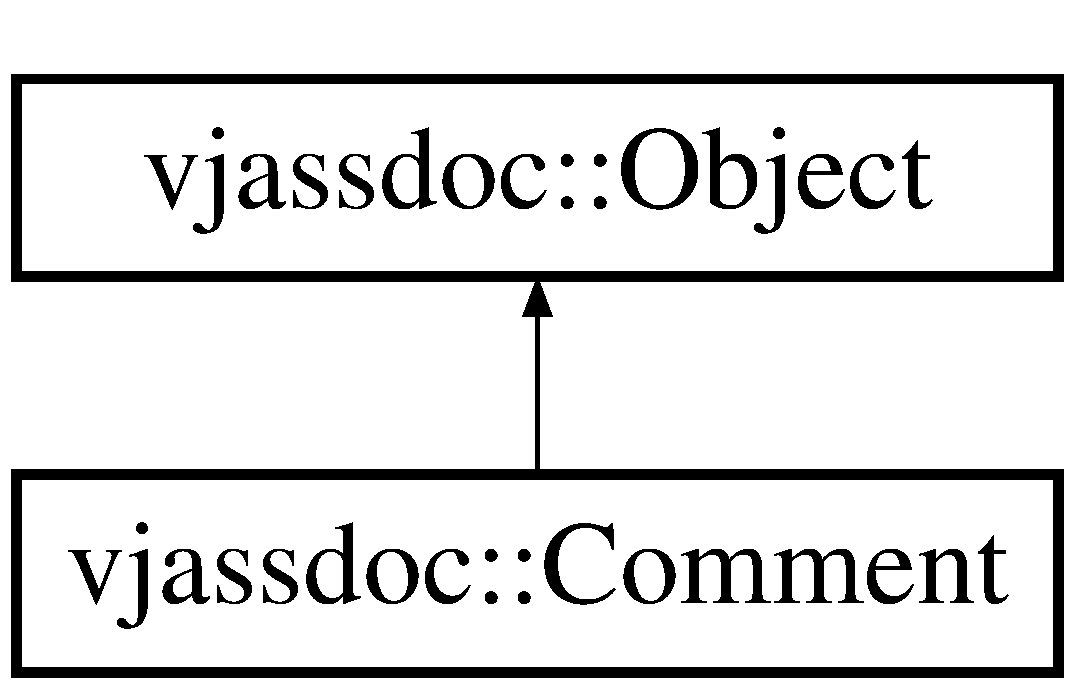
\includegraphics[height=2cm]{classvjassdoc_1_1Comment}
\end{center}
\end{figure}
\subsection*{Public Member Functions}
\begin{CompactItemize}
\item 
\hyperlink{classvjassdoc_1_1Comment_5f0e466f9d476c67442ada31ea51840e}{Comment} (const std::string \&identifier, class \hyperlink{classvjassdoc_1_1SourceFile}{SourceFile} $\ast$sourceFile, unsigned int line, class \hyperlink{classvjassdoc_1_1DocComment}{DocComment} $\ast$docComment)
\item 
\hyperlink{classvjassdoc_1_1Comment_ba8561a5b6e39538356e21e7edf93432}{Comment} (std::vector$<$ const unsigned char $\ast$ $>$ \&columnVector)
\item 
virtual \hyperlink{classvjassdoc_1_1Comment_97211d4a9d951c8eed8061c5e7a518b8}{$\sim$Comment} ()
\item 
virtual void \hyperlink{classvjassdoc_1_1Comment_07ad51bf42ce397832b77eb96379c054}{init} ()
\item 
virtual void \hyperlink{classvjassdoc_1_1Comment_4bcb5f83071ad7954b922fdaf8e0ea8e}{pageNavigation} (std::ofstream \&file) const 
\item 
virtual void \hyperlink{classvjassdoc_1_1Comment_d7b59c02557b961deb2f470b180bab7a}{page} (std::ofstream \&file) const 
\end{CompactItemize}


\subsection{Constructor \& Destructor Documentation}
\hypertarget{classvjassdoc_1_1Comment_5f0e466f9d476c67442ada31ea51840e}{
\index{vjassdoc::Comment@{vjassdoc::Comment}!Comment@{Comment}}
\index{Comment@{Comment}!vjassdoc::Comment@{vjassdoc::Comment}}
\subsubsection{\setlength{\rightskip}{0pt plus 5cm}vjassdoc::Comment::Comment (const std::string \& {\em identifier}, class {\bf SourceFile} $\ast$ {\em sourceFile}, unsigned int {\em line}, class {\bf DocComment} $\ast$ {\em docComment})}}
\label{classvjassdoc_1_1Comment_5f0e466f9d476c67442ada31ea51840e}


\hypertarget{classvjassdoc_1_1Comment_ba8561a5b6e39538356e21e7edf93432}{
\index{vjassdoc::Comment@{vjassdoc::Comment}!Comment@{Comment}}
\index{Comment@{Comment}!vjassdoc::Comment@{vjassdoc::Comment}}
\subsubsection{\setlength{\rightskip}{0pt plus 5cm}vjassdoc::Comment::Comment (std::vector$<$ const unsigned char $\ast$ $>$ \& {\em columnVector})}}
\label{classvjassdoc_1_1Comment_ba8561a5b6e39538356e21e7edf93432}


\hypertarget{classvjassdoc_1_1Comment_97211d4a9d951c8eed8061c5e7a518b8}{
\index{vjassdoc::Comment@{vjassdoc::Comment}!$\sim$Comment@{$\sim$Comment}}
\index{$\sim$Comment@{$\sim$Comment}!vjassdoc::Comment@{vjassdoc::Comment}}
\subsubsection{\setlength{\rightskip}{0pt plus 5cm}vjassdoc::Comment::$\sim$Comment ()\hspace{0.3cm}{\tt  \mbox{[}virtual\mbox{]}}}}
\label{classvjassdoc_1_1Comment_97211d4a9d951c8eed8061c5e7a518b8}




\subsection{Member Function Documentation}
\hypertarget{classvjassdoc_1_1Comment_07ad51bf42ce397832b77eb96379c054}{
\index{vjassdoc::Comment@{vjassdoc::Comment}!init@{init}}
\index{init@{init}!vjassdoc::Comment@{vjassdoc::Comment}}
\subsubsection{\setlength{\rightskip}{0pt plus 5cm}void vjassdoc::Comment::init ()\hspace{0.3cm}{\tt  \mbox{[}virtual\mbox{]}}}}
\label{classvjassdoc_1_1Comment_07ad51bf42ce397832b77eb96379c054}




Implements \hyperlink{classvjassdoc_1_1Object_bd43e77dbe80055f5adda67661dfaca4}{vjassdoc::Object}.\hypertarget{classvjassdoc_1_1Comment_4bcb5f83071ad7954b922fdaf8e0ea8e}{
\index{vjassdoc::Comment@{vjassdoc::Comment}!pageNavigation@{pageNavigation}}
\index{pageNavigation@{pageNavigation}!vjassdoc::Comment@{vjassdoc::Comment}}
\subsubsection{\setlength{\rightskip}{0pt plus 5cm}void vjassdoc::Comment::pageNavigation (std::ofstream \& {\em file}) const\hspace{0.3cm}{\tt  \mbox{[}virtual\mbox{]}}}}
\label{classvjassdoc_1_1Comment_4bcb5f83071ad7954b922fdaf8e0ea8e}




Implements \hyperlink{classvjassdoc_1_1Object_736bbb6719edd8070d8f56c364a2764c}{vjassdoc::Object}.\hypertarget{classvjassdoc_1_1Comment_d7b59c02557b961deb2f470b180bab7a}{
\index{vjassdoc::Comment@{vjassdoc::Comment}!page@{page}}
\index{page@{page}!vjassdoc::Comment@{vjassdoc::Comment}}
\subsubsection{\setlength{\rightskip}{0pt plus 5cm}void vjassdoc::Comment::page (std::ofstream \& {\em file}) const\hspace{0.3cm}{\tt  \mbox{[}virtual\mbox{]}}}}
\label{classvjassdoc_1_1Comment_d7b59c02557b961deb2f470b180bab7a}




Implements \hyperlink{classvjassdoc_1_1Object_a0489e38956f3507566b1bc6e3e2c8af}{vjassdoc::Object}.

The documentation for this class was generated from the following files:\begin{CompactItemize}
\item 
src/\hyperlink{comment_8h}{comment.h}\item 
src/\hyperlink{comment_8cpp}{comment.cpp}\end{CompactItemize}

\hypertarget{classvjassdoc_1_1DocComment}{
\section{vjassdoc::DocComment Class Reference}
\label{classvjassdoc_1_1DocComment}\index{vjassdoc::DocComment@{vjassdoc::DocComment}}
}
{\tt \#include $<$doccomment.h$>$}

Inheritance diagram for vjassdoc::DocComment::\begin{figure}[H]
\begin{center}
\leavevmode
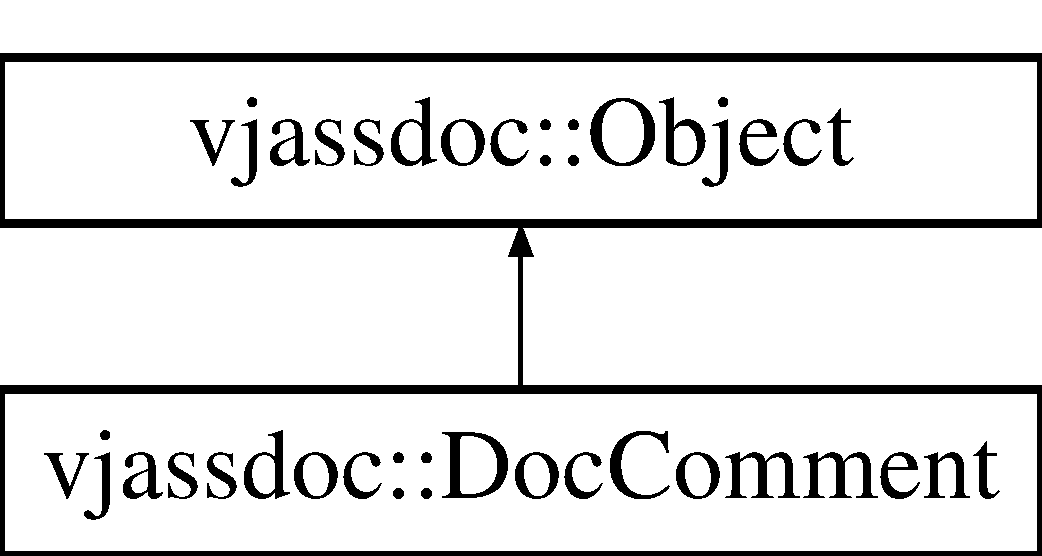
\includegraphics[height=2cm]{classvjassdoc_1_1DocComment}
\end{center}
\end{figure}
\subsection*{Public Member Functions}
\begin{CompactItemize}
\item 
\hyperlink{classvjassdoc_1_1DocComment_1a3724cee4e159efbac83c6c6e163301}{DocComment} (const std::string \&identifier, class \hyperlink{classvjassdoc_1_1SourceFile}{SourceFile} $\ast$sourceFile, unsigned int line)
\item 
\hyperlink{classvjassdoc_1_1DocComment_cc620c22e37f63571e20991a8f077ea3}{DocComment} (std::vector$<$ const unsigned char $\ast$ $>$ \&columnVector)
\item 
virtual void \hyperlink{classvjassdoc_1_1DocComment_46ada773166611c9be898f74e0eb2315}{init} ()
\item 
virtual void \hyperlink{classvjassdoc_1_1DocComment_2a0b017c17c8a20679b2052b87a74c15}{pageNavigation} (std::ofstream \&file) const 
\item 
virtual void \hyperlink{classvjassdoc_1_1DocComment_79dd94421713887af6028f49736d895d}{page} (std::ofstream \&file) const 
\item 
virtual std::string \hyperlink{classvjassdoc_1_1DocComment_d50177b6a9bd805ebe1ef76b8607242e}{sqlStatement} () const 
\item 
void \hyperlink{classvjassdoc_1_1DocComment_486dc09c43432be8e8285716aad13607}{setObject} (class \hyperlink{classvjassdoc_1_1Object}{Object} $\ast$object)
\item 
class \hyperlink{classvjassdoc_1_1Object}{Object} $\ast$ \hyperlink{classvjassdoc_1_1DocComment_057c80a5fd3a3c7d776483feaf51a8a8}{object} () const 
\end{CompactItemize}


\subsection{Constructor \& Destructor Documentation}
\hypertarget{classvjassdoc_1_1DocComment_1a3724cee4e159efbac83c6c6e163301}{
\index{vjassdoc::DocComment@{vjassdoc::DocComment}!DocComment@{DocComment}}
\index{DocComment@{DocComment}!vjassdoc::DocComment@{vjassdoc::DocComment}}
\subsubsection{\setlength{\rightskip}{0pt plus 5cm}vjassdoc::DocComment::DocComment (const std::string \& {\em identifier}, class {\bf SourceFile} $\ast$ {\em sourceFile}, unsigned int {\em line})}}
\label{classvjassdoc_1_1DocComment_1a3724cee4e159efbac83c6c6e163301}


\hypertarget{classvjassdoc_1_1DocComment_cc620c22e37f63571e20991a8f077ea3}{
\index{vjassdoc::DocComment@{vjassdoc::DocComment}!DocComment@{DocComment}}
\index{DocComment@{DocComment}!vjassdoc::DocComment@{vjassdoc::DocComment}}
\subsubsection{\setlength{\rightskip}{0pt plus 5cm}vjassdoc::DocComment::DocComment (std::vector$<$ const unsigned char $\ast$ $>$ \& {\em columnVector})}}
\label{classvjassdoc_1_1DocComment_cc620c22e37f63571e20991a8f077ea3}




\subsection{Member Function Documentation}
\hypertarget{classvjassdoc_1_1DocComment_46ada773166611c9be898f74e0eb2315}{
\index{vjassdoc::DocComment@{vjassdoc::DocComment}!init@{init}}
\index{init@{init}!vjassdoc::DocComment@{vjassdoc::DocComment}}
\subsubsection{\setlength{\rightskip}{0pt plus 5cm}void vjassdoc::DocComment::init ()\hspace{0.3cm}{\tt  \mbox{[}virtual\mbox{]}}}}
\label{classvjassdoc_1_1DocComment_46ada773166611c9be898f74e0eb2315}


\begin{Desc}
\item[\hyperlink{todo__todo000001}{Todo}]FIXME \end{Desc}


Implements \hyperlink{classvjassdoc_1_1Object_bd43e77dbe80055f5adda67661dfaca4}{vjassdoc::Object}.\hypertarget{classvjassdoc_1_1DocComment_2a0b017c17c8a20679b2052b87a74c15}{
\index{vjassdoc::DocComment@{vjassdoc::DocComment}!pageNavigation@{pageNavigation}}
\index{pageNavigation@{pageNavigation}!vjassdoc::DocComment@{vjassdoc::DocComment}}
\subsubsection{\setlength{\rightskip}{0pt plus 5cm}void vjassdoc::DocComment::pageNavigation (std::ofstream \& {\em file}) const\hspace{0.3cm}{\tt  \mbox{[}virtual\mbox{]}}}}
\label{classvjassdoc_1_1DocComment_2a0b017c17c8a20679b2052b87a74c15}




Implements \hyperlink{classvjassdoc_1_1Object_736bbb6719edd8070d8f56c364a2764c}{vjassdoc::Object}.\hypertarget{classvjassdoc_1_1DocComment_79dd94421713887af6028f49736d895d}{
\index{vjassdoc::DocComment@{vjassdoc::DocComment}!page@{page}}
\index{page@{page}!vjassdoc::DocComment@{vjassdoc::DocComment}}
\subsubsection{\setlength{\rightskip}{0pt plus 5cm}void vjassdoc::DocComment::page (std::ofstream \& {\em file}) const\hspace{0.3cm}{\tt  \mbox{[}virtual\mbox{]}}}}
\label{classvjassdoc_1_1DocComment_79dd94421713887af6028f49736d895d}




Implements \hyperlink{classvjassdoc_1_1Object_a0489e38956f3507566b1bc6e3e2c8af}{vjassdoc::Object}.\hypertarget{classvjassdoc_1_1DocComment_d50177b6a9bd805ebe1ef76b8607242e}{
\index{vjassdoc::DocComment@{vjassdoc::DocComment}!sqlStatement@{sqlStatement}}
\index{sqlStatement@{sqlStatement}!vjassdoc::DocComment@{vjassdoc::DocComment}}
\subsubsection{\setlength{\rightskip}{0pt plus 5cm}std::string vjassdoc::DocComment::sqlStatement () const\hspace{0.3cm}{\tt  \mbox{[}virtual\mbox{]}}}}
\label{classvjassdoc_1_1DocComment_d50177b6a9bd805ebe1ef76b8607242e}




Reimplemented from \hyperlink{classvjassdoc_1_1Object_4e8ebbb0ce5b0bf91ec847b1e4a9f8fc}{vjassdoc::Object}.\hypertarget{classvjassdoc_1_1DocComment_486dc09c43432be8e8285716aad13607}{
\index{vjassdoc::DocComment@{vjassdoc::DocComment}!setObject@{setObject}}
\index{setObject@{setObject}!vjassdoc::DocComment@{vjassdoc::DocComment}}
\subsubsection{\setlength{\rightskip}{0pt plus 5cm}void vjassdoc::DocComment::setObject (class {\bf Object} $\ast$ {\em object})\hspace{0.3cm}{\tt  \mbox{[}inline\mbox{]}}}}
\label{classvjassdoc_1_1DocComment_486dc09c43432be8e8285716aad13607}


\hypertarget{classvjassdoc_1_1DocComment_057c80a5fd3a3c7d776483feaf51a8a8}{
\index{vjassdoc::DocComment@{vjassdoc::DocComment}!object@{object}}
\index{object@{object}!vjassdoc::DocComment@{vjassdoc::DocComment}}
\subsubsection{\setlength{\rightskip}{0pt plus 5cm}class {\bf Object} $\ast$ vjassdoc::DocComment::object () const\hspace{0.3cm}{\tt  \mbox{[}inline\mbox{]}}}}
\label{classvjassdoc_1_1DocComment_057c80a5fd3a3c7d776483feaf51a8a8}




The documentation for this class was generated from the following files:\begin{CompactItemize}
\item 
src/\hyperlink{doccomment_8h}{doccomment.h}\item 
src/\hyperlink{doccomment_8cpp}{doccomment.cpp}\end{CompactItemize}

\hypertarget{classvjassdoc_1_1File}{
\section{vjassdoc::File Class Reference}
\label{classvjassdoc_1_1File}\index{vjassdoc::File@{vjassdoc::File}}
}
{\tt \#include $<$file.h$>$}

\subsection*{Public Types}
\begin{CompactItemize}
\item 
enum \hyperlink{classvjassdoc_1_1File_78479b8cb631d0db80ba984da1781265}{Expression} \{ \par
\hyperlink{classvjassdoc_1_1File_78479b8cb631d0db80ba984da17812651b865eb7837fa58aa48ea6e0db11aef3}{PreprocessorExpression}, 
\hyperlink{classvjassdoc_1_1File_78479b8cb631d0db80ba984da1781265b4a9c2519ee43d16d4037f75a67cad0a}{DocCommentExpression}, 
\hyperlink{classvjassdoc_1_1File_78479b8cb631d0db80ba984da17812651eb711a77df439eca7d9c35ae6b61fc2}{CommentExpression}, 
\hyperlink{classvjassdoc_1_1File_78479b8cb631d0db80ba984da17812653e8a9b6e963deb6df9c8fe3625b51a8d}{TypeExpression}, 
\par
\hyperlink{classvjassdoc_1_1File_78479b8cb631d0db80ba984da17812654058cc2c8a8c9723fd45766e631d9e0e}{ConstantExpression}, 
\hyperlink{classvjassdoc_1_1File_78479b8cb631d0db80ba984da1781265695caaefe6d8b5a21559bdfeecf8cec8}{ExtendsExpression}, 
\hyperlink{classvjassdoc_1_1File_78479b8cb631d0db80ba984da17812655e40c3e6596bebee34de6c44c9d9bcec}{NativeExpression}, 
\hyperlink{classvjassdoc_1_1File_78479b8cb631d0db80ba984da178126595e0227e32402f65db935d12a7bcb5e4}{NothingExpression}, 
\par
\hyperlink{classvjassdoc_1_1File_78479b8cb631d0db80ba984da1781265cc522891e16a6cc75c211607a6325ebe}{FunctionExpression}, 
\hyperlink{classvjassdoc_1_1File_78479b8cb631d0db80ba984da1781265e98a592745ca3714c40ebf465979eb72}{EndfunctionExpression}, 
\hyperlink{classvjassdoc_1_1File_78479b8cb631d0db80ba984da1781265486a35a903ff1266cd7dc58edfcdedcc}{TakesExpression}, 
\hyperlink{classvjassdoc_1_1File_78479b8cb631d0db80ba984da178126562a370dd1e411e75df2a184517e68816}{ReturnsExpression}, 
\par
\hyperlink{classvjassdoc_1_1File_78479b8cb631d0db80ba984da1781265115a4523bd4b2d6c5ba29ecfe50ac779}{GlobalsExpression}, 
\hyperlink{classvjassdoc_1_1File_78479b8cb631d0db80ba984da1781265800e41973cb47a647ab273fd03c75963}{EndglobalsExpression}, 
\hyperlink{classvjassdoc_1_1File_78479b8cb631d0db80ba984da1781265e5edf96ada5e20813ea370cc67277ddb}{ImportExpression}, 
\hyperlink{classvjassdoc_1_1File_78479b8cb631d0db80ba984da1781265bf9654d71948af3c0be78dfed55a1ea9}{DovjassinitExpression}, 
\par
\hyperlink{classvjassdoc_1_1File_78479b8cb631d0db80ba984da178126549f2632d9d7e3eb147dbba9359d90723}{InjectExpression}, 
\hyperlink{classvjassdoc_1_1File_78479b8cb631d0db80ba984da178126592cfd654247d69f6e96ff1ac0a9113ec}{EndinjectExpression}, 
\hyperlink{classvjassdoc_1_1File_78479b8cb631d0db80ba984da17812653bbfac25fb8eeee6e9c1885aaccd8fce}{NovjassExpression}, 
\hyperlink{classvjassdoc_1_1File_78479b8cb631d0db80ba984da17812653447311b46995fdb928034c7b29fde26}{EndnovjassExpression}, 
\par
\hyperlink{classvjassdoc_1_1File_78479b8cb631d0db80ba984da178126511949bc219458e42396ce0fe022b7b79}{LoaddataExpression}, 
\hyperlink{classvjassdoc_1_1File_78479b8cb631d0db80ba984da1781265d517452d79e6a72b7c1b0c403683177b}{ExternalExpression}, 
\hyperlink{classvjassdoc_1_1File_78479b8cb631d0db80ba984da17812655de93252f22a90465e4af610ba28937d}{TextmacroExpression}, 
\hyperlink{classvjassdoc_1_1File_78479b8cb631d0db80ba984da178126508a99e55915dd4349c64b45ed384a1d7}{EndtextmacroExpression}, 
\par
\hyperlink{classvjassdoc_1_1File_78479b8cb631d0db80ba984da17812655a243219a44a4273f04e891080711599}{RuntextmacroExpression}, 
\hyperlink{classvjassdoc_1_1File_78479b8cb631d0db80ba984da178126562c7c9c2ccef86c8606c83e566f8fc4d}{RequiresExpression}, 
\hyperlink{classvjassdoc_1_1File_78479b8cb631d0db80ba984da178126592307eaed8ccaca61ae97a3d66c00705}{NeedsExpression}, 
\hyperlink{classvjassdoc_1_1File_78479b8cb631d0db80ba984da178126523e0fb9c8a4d230ff2bade2a53913fcc}{UsesExpression}, 
\par
\hyperlink{classvjassdoc_1_1File_78479b8cb631d0db80ba984da178126560f9a23d8773c97ee5e2d24c460227f5}{InitializerExpression}, 
\hyperlink{classvjassdoc_1_1File_78479b8cb631d0db80ba984da1781265023ea144c4fcfe57b213d37e4465bdf1}{DefaultsExpression}, 
\hyperlink{classvjassdoc_1_1File_78479b8cb631d0db80ba984da178126523543fae882fc1d836c26e7980b586df}{MethodExpression}, 
\hyperlink{classvjassdoc_1_1File_78479b8cb631d0db80ba984da1781265df09a795fc606410fc5ace66ca7beb38}{EndmethodExpression}, 
\par
\hyperlink{classvjassdoc_1_1File_78479b8cb631d0db80ba984da17812654106bf220b5490dce30f389f2a2e9f99}{PrivateExpression}, 
\hyperlink{classvjassdoc_1_1File_78479b8cb631d0db80ba984da1781265d578f3d8f81442a668b749a030b0354c}{PublicExpression}, 
\hyperlink{classvjassdoc_1_1File_78479b8cb631d0db80ba984da17812658b842db48a1f5975841f191cd0c57705}{StaticExpression}, 
\hyperlink{classvjassdoc_1_1File_78479b8cb631d0db80ba984da178126559f1e70c098ac65b713eae32d4550019}{DebugExpression}, 
\par
\hyperlink{classvjassdoc_1_1File_78479b8cb631d0db80ba984da17812658b8a022c5e0f3aaafc065484f82a19ed}{KeywordExpression}, 
\hyperlink{classvjassdoc_1_1File_78479b8cb631d0db80ba984da1781265526c3fad85e36e729c328a402421dc3d}{LibraryExpression}, 
\hyperlink{classvjassdoc_1_1File_78479b8cb631d0db80ba984da1781265a2b4de2d0a50961ca50bfa594c8fbc5b}{Library\_\-onceExpression}, 
\hyperlink{classvjassdoc_1_1File_78479b8cb631d0db80ba984da178126534feae053c2cd8651477e57b1c92fe49}{EndlibraryExpression}, 
\par
\hyperlink{classvjassdoc_1_1File_78479b8cb631d0db80ba984da1781265676e75bb41276fab0df86c719390c93b}{ScopeExpression}, 
\hyperlink{classvjassdoc_1_1File_78479b8cb631d0db80ba984da17812650a32b747c1a465c595fcfa9542ed5df1}{EndscopeExpression}, 
\hyperlink{classvjassdoc_1_1File_78479b8cb631d0db80ba984da17812655f466775916687b49e9458ffd1cf175f}{StructExpression}, 
\hyperlink{classvjassdoc_1_1File_78479b8cb631d0db80ba984da1781265769434b43217cbf4578036fbb0e0c40f}{EndstructExpression}, 
\par
\hyperlink{classvjassdoc_1_1File_78479b8cb631d0db80ba984da1781265739141f9b85648b53536e2317e4e761d}{InterfaceExpression}, 
\hyperlink{classvjassdoc_1_1File_78479b8cb631d0db80ba984da1781265bd069d08c5de7b98115ce911967ba4e5}{EndinterfaceExpression}, 
\hyperlink{classvjassdoc_1_1File_78479b8cb631d0db80ba984da1781265ba68399edf35cf80436d386e6034e565}{DelegateExpression}, 
\hyperlink{classvjassdoc_1_1File_78479b8cb631d0db80ba984da17812651af4094ba3881a0352822fd855d7a619}{StubExpression}, 
\par
\hyperlink{classvjassdoc_1_1File_78479b8cb631d0db80ba984da1781265d38085c3df5b961eb4412adaad722f4e}{ArrayExpression}, 
\hyperlink{classvjassdoc_1_1File_78479b8cb631d0db80ba984da1781265dfba3c7f05cebee4414db0ab14f2860b}{MaxExpressions}
 \}
\item 
enum \hyperlink{classvjassdoc_1_1File_3126530fe28afe1ed99bf67e86a56ab8}{DocExpression} \{ \par
\hyperlink{classvjassdoc_1_1File_3126530fe28afe1ed99bf67e86a56ab8566e293faddbb103f42103d4cab0f58a}{Author}, 
\hyperlink{classvjassdoc_1_1File_3126530fe28afe1ed99bf67e86a56ab8674ae9cfc32ac1b9bf1ed906c0e96d8a}{ToDo}, 
\hyperlink{classvjassdoc_1_1File_3126530fe28afe1ed99bf67e86a56ab82b3e070b478db15d95689af849273e7c}{Parameter}, 
\hyperlink{classvjassdoc_1_1File_3126530fe28afe1ed99bf67e86a56ab8614d5af138e60bf61e65e2521b1cdb42}{Return}, 
\par
\hyperlink{classvjassdoc_1_1File_3126530fe28afe1ed99bf67e86a56ab8bf7b26b18788d06147da03303daf2b0b}{State}, 
\hyperlink{classvjassdoc_1_1File_3126530fe28afe1ed99bf67e86a56ab86a0a5002e255e5a3c600139561fc4736}{Source}, 
\hyperlink{classvjassdoc_1_1File_3126530fe28afe1ed99bf67e86a56ab8e2ba12169a4184b99fcd6ed350055a58}{MaxDocExpressions}
 \}
\end{CompactItemize}
\subsection*{Public Member Functions}
\begin{CompactItemize}
\item 
\hyperlink{classvjassdoc_1_1File_d35f0f273a4e7ecc96e4315edb842151}{File} (const std::string \&filePath)
\end{CompactItemize}
\subsection*{Static Public Member Functions}
\begin{CompactItemize}
\item 
static std::string \hyperlink{classvjassdoc_1_1File_424079db72abbc4c6812691748c10362}{getToken} (const std::string \&line, unsigned int \&index, bool endOfLine=false)
\end{CompactItemize}
\subsection*{Static Public Attributes}
\begin{CompactItemize}
\item 
static const char $\ast$ \hyperlink{classvjassdoc_1_1File_bcc699454548ae47f02ca6cdf6b333ab}{expressionText} \mbox{[}File::MaxExpressions\mbox{]}
\item 
static const char $\ast$ \hyperlink{classvjassdoc_1_1File_399e6e8a31347b0f354727874a825c34}{docExpressionText} \mbox{[}File::MaxDocExpressions\mbox{]}
\end{CompactItemize}


\subsection{Member Enumeration Documentation}
\hypertarget{classvjassdoc_1_1File_78479b8cb631d0db80ba984da1781265}{
\index{vjassdoc::File@{vjassdoc::File}!Expression@{Expression}}
\index{Expression@{Expression}!vjassdoc::File@{vjassdoc::File}}
\subsubsection{\setlength{\rightskip}{0pt plus 5cm}enum {\bf vjassdoc::File::Expression}}}
\label{classvjassdoc_1_1File_78479b8cb631d0db80ba984da1781265}


\begin{Desc}
\item[Enumerator: ]\par
\begin{description}
\index{PreprocessorExpression@{PreprocessorExpression}!vjassdoc::File@{vjassdoc::File}}\index{vjassdoc::File@{vjassdoc::File}!PreprocessorExpression@{PreprocessorExpression}}\item[{\em 
\hypertarget{classvjassdoc_1_1File_78479b8cb631d0db80ba984da17812651b865eb7837fa58aa48ea6e0db11aef3}{
PreprocessorExpression}
\label{classvjassdoc_1_1File_78479b8cb631d0db80ba984da17812651b865eb7837fa58aa48ea6e0db11aef3}
}]\index{DocCommentExpression@{DocCommentExpression}!vjassdoc::File@{vjassdoc::File}}\index{vjassdoc::File@{vjassdoc::File}!DocCommentExpression@{DocCommentExpression}}\item[{\em 
\hypertarget{classvjassdoc_1_1File_78479b8cb631d0db80ba984da1781265b4a9c2519ee43d16d4037f75a67cad0a}{
DocCommentExpression}
\label{classvjassdoc_1_1File_78479b8cb631d0db80ba984da1781265b4a9c2519ee43d16d4037f75a67cad0a}
}]\index{CommentExpression@{CommentExpression}!vjassdoc::File@{vjassdoc::File}}\index{vjassdoc::File@{vjassdoc::File}!CommentExpression@{CommentExpression}}\item[{\em 
\hypertarget{classvjassdoc_1_1File_78479b8cb631d0db80ba984da17812651eb711a77df439eca7d9c35ae6b61fc2}{
CommentExpression}
\label{classvjassdoc_1_1File_78479b8cb631d0db80ba984da17812651eb711a77df439eca7d9c35ae6b61fc2}
}]\index{TypeExpression@{TypeExpression}!vjassdoc::File@{vjassdoc::File}}\index{vjassdoc::File@{vjassdoc::File}!TypeExpression@{TypeExpression}}\item[{\em 
\hypertarget{classvjassdoc_1_1File_78479b8cb631d0db80ba984da17812653e8a9b6e963deb6df9c8fe3625b51a8d}{
TypeExpression}
\label{classvjassdoc_1_1File_78479b8cb631d0db80ba984da17812653e8a9b6e963deb6df9c8fe3625b51a8d}
}]\index{ConstantExpression@{ConstantExpression}!vjassdoc::File@{vjassdoc::File}}\index{vjassdoc::File@{vjassdoc::File}!ConstantExpression@{ConstantExpression}}\item[{\em 
\hypertarget{classvjassdoc_1_1File_78479b8cb631d0db80ba984da17812654058cc2c8a8c9723fd45766e631d9e0e}{
ConstantExpression}
\label{classvjassdoc_1_1File_78479b8cb631d0db80ba984da17812654058cc2c8a8c9723fd45766e631d9e0e}
}]\index{ExtendsExpression@{ExtendsExpression}!vjassdoc::File@{vjassdoc::File}}\index{vjassdoc::File@{vjassdoc::File}!ExtendsExpression@{ExtendsExpression}}\item[{\em 
\hypertarget{classvjassdoc_1_1File_78479b8cb631d0db80ba984da1781265695caaefe6d8b5a21559bdfeecf8cec8}{
ExtendsExpression}
\label{classvjassdoc_1_1File_78479b8cb631d0db80ba984da1781265695caaefe6d8b5a21559bdfeecf8cec8}
}]\index{NativeExpression@{NativeExpression}!vjassdoc::File@{vjassdoc::File}}\index{vjassdoc::File@{vjassdoc::File}!NativeExpression@{NativeExpression}}\item[{\em 
\hypertarget{classvjassdoc_1_1File_78479b8cb631d0db80ba984da17812655e40c3e6596bebee34de6c44c9d9bcec}{
NativeExpression}
\label{classvjassdoc_1_1File_78479b8cb631d0db80ba984da17812655e40c3e6596bebee34de6c44c9d9bcec}
}]\index{NothingExpression@{NothingExpression}!vjassdoc::File@{vjassdoc::File}}\index{vjassdoc::File@{vjassdoc::File}!NothingExpression@{NothingExpression}}\item[{\em 
\hypertarget{classvjassdoc_1_1File_78479b8cb631d0db80ba984da178126595e0227e32402f65db935d12a7bcb5e4}{
NothingExpression}
\label{classvjassdoc_1_1File_78479b8cb631d0db80ba984da178126595e0227e32402f65db935d12a7bcb5e4}
}]\index{FunctionExpression@{FunctionExpression}!vjassdoc::File@{vjassdoc::File}}\index{vjassdoc::File@{vjassdoc::File}!FunctionExpression@{FunctionExpression}}\item[{\em 
\hypertarget{classvjassdoc_1_1File_78479b8cb631d0db80ba984da1781265cc522891e16a6cc75c211607a6325ebe}{
FunctionExpression}
\label{classvjassdoc_1_1File_78479b8cb631d0db80ba984da1781265cc522891e16a6cc75c211607a6325ebe}
}]\index{EndfunctionExpression@{EndfunctionExpression}!vjassdoc::File@{vjassdoc::File}}\index{vjassdoc::File@{vjassdoc::File}!EndfunctionExpression@{EndfunctionExpression}}\item[{\em 
\hypertarget{classvjassdoc_1_1File_78479b8cb631d0db80ba984da1781265e98a592745ca3714c40ebf465979eb72}{
EndfunctionExpression}
\label{classvjassdoc_1_1File_78479b8cb631d0db80ba984da1781265e98a592745ca3714c40ebf465979eb72}
}]\index{TakesExpression@{TakesExpression}!vjassdoc::File@{vjassdoc::File}}\index{vjassdoc::File@{vjassdoc::File}!TakesExpression@{TakesExpression}}\item[{\em 
\hypertarget{classvjassdoc_1_1File_78479b8cb631d0db80ba984da1781265486a35a903ff1266cd7dc58edfcdedcc}{
TakesExpression}
\label{classvjassdoc_1_1File_78479b8cb631d0db80ba984da1781265486a35a903ff1266cd7dc58edfcdedcc}
}]\index{ReturnsExpression@{ReturnsExpression}!vjassdoc::File@{vjassdoc::File}}\index{vjassdoc::File@{vjassdoc::File}!ReturnsExpression@{ReturnsExpression}}\item[{\em 
\hypertarget{classvjassdoc_1_1File_78479b8cb631d0db80ba984da178126562a370dd1e411e75df2a184517e68816}{
ReturnsExpression}
\label{classvjassdoc_1_1File_78479b8cb631d0db80ba984da178126562a370dd1e411e75df2a184517e68816}
}]\index{GlobalsExpression@{GlobalsExpression}!vjassdoc::File@{vjassdoc::File}}\index{vjassdoc::File@{vjassdoc::File}!GlobalsExpression@{GlobalsExpression}}\item[{\em 
\hypertarget{classvjassdoc_1_1File_78479b8cb631d0db80ba984da1781265115a4523bd4b2d6c5ba29ecfe50ac779}{
GlobalsExpression}
\label{classvjassdoc_1_1File_78479b8cb631d0db80ba984da1781265115a4523bd4b2d6c5ba29ecfe50ac779}
}]\index{EndglobalsExpression@{EndglobalsExpression}!vjassdoc::File@{vjassdoc::File}}\index{vjassdoc::File@{vjassdoc::File}!EndglobalsExpression@{EndglobalsExpression}}\item[{\em 
\hypertarget{classvjassdoc_1_1File_78479b8cb631d0db80ba984da1781265800e41973cb47a647ab273fd03c75963}{
EndglobalsExpression}
\label{classvjassdoc_1_1File_78479b8cb631d0db80ba984da1781265800e41973cb47a647ab273fd03c75963}
}]\index{ImportExpression@{ImportExpression}!vjassdoc::File@{vjassdoc::File}}\index{vjassdoc::File@{vjassdoc::File}!ImportExpression@{ImportExpression}}\item[{\em 
\hypertarget{classvjassdoc_1_1File_78479b8cb631d0db80ba984da1781265e5edf96ada5e20813ea370cc67277ddb}{
ImportExpression}
\label{classvjassdoc_1_1File_78479b8cb631d0db80ba984da1781265e5edf96ada5e20813ea370cc67277ddb}
}]\index{DovjassinitExpression@{DovjassinitExpression}!vjassdoc::File@{vjassdoc::File}}\index{vjassdoc::File@{vjassdoc::File}!DovjassinitExpression@{DovjassinitExpression}}\item[{\em 
\hypertarget{classvjassdoc_1_1File_78479b8cb631d0db80ba984da1781265bf9654d71948af3c0be78dfed55a1ea9}{
DovjassinitExpression}
\label{classvjassdoc_1_1File_78479b8cb631d0db80ba984da1781265bf9654d71948af3c0be78dfed55a1ea9}
}]\index{InjectExpression@{InjectExpression}!vjassdoc::File@{vjassdoc::File}}\index{vjassdoc::File@{vjassdoc::File}!InjectExpression@{InjectExpression}}\item[{\em 
\hypertarget{classvjassdoc_1_1File_78479b8cb631d0db80ba984da178126549f2632d9d7e3eb147dbba9359d90723}{
InjectExpression}
\label{classvjassdoc_1_1File_78479b8cb631d0db80ba984da178126549f2632d9d7e3eb147dbba9359d90723}
}]\index{EndinjectExpression@{EndinjectExpression}!vjassdoc::File@{vjassdoc::File}}\index{vjassdoc::File@{vjassdoc::File}!EndinjectExpression@{EndinjectExpression}}\item[{\em 
\hypertarget{classvjassdoc_1_1File_78479b8cb631d0db80ba984da178126592cfd654247d69f6e96ff1ac0a9113ec}{
EndinjectExpression}
\label{classvjassdoc_1_1File_78479b8cb631d0db80ba984da178126592cfd654247d69f6e96ff1ac0a9113ec}
}]\index{NovjassExpression@{NovjassExpression}!vjassdoc::File@{vjassdoc::File}}\index{vjassdoc::File@{vjassdoc::File}!NovjassExpression@{NovjassExpression}}\item[{\em 
\hypertarget{classvjassdoc_1_1File_78479b8cb631d0db80ba984da17812653bbfac25fb8eeee6e9c1885aaccd8fce}{
NovjassExpression}
\label{classvjassdoc_1_1File_78479b8cb631d0db80ba984da17812653bbfac25fb8eeee6e9c1885aaccd8fce}
}]\index{EndnovjassExpression@{EndnovjassExpression}!vjassdoc::File@{vjassdoc::File}}\index{vjassdoc::File@{vjassdoc::File}!EndnovjassExpression@{EndnovjassExpression}}\item[{\em 
\hypertarget{classvjassdoc_1_1File_78479b8cb631d0db80ba984da17812653447311b46995fdb928034c7b29fde26}{
EndnovjassExpression}
\label{classvjassdoc_1_1File_78479b8cb631d0db80ba984da17812653447311b46995fdb928034c7b29fde26}
}]\index{LoaddataExpression@{LoaddataExpression}!vjassdoc::File@{vjassdoc::File}}\index{vjassdoc::File@{vjassdoc::File}!LoaddataExpression@{LoaddataExpression}}\item[{\em 
\hypertarget{classvjassdoc_1_1File_78479b8cb631d0db80ba984da178126511949bc219458e42396ce0fe022b7b79}{
LoaddataExpression}
\label{classvjassdoc_1_1File_78479b8cb631d0db80ba984da178126511949bc219458e42396ce0fe022b7b79}
}]\index{ExternalExpression@{ExternalExpression}!vjassdoc::File@{vjassdoc::File}}\index{vjassdoc::File@{vjassdoc::File}!ExternalExpression@{ExternalExpression}}\item[{\em 
\hypertarget{classvjassdoc_1_1File_78479b8cb631d0db80ba984da1781265d517452d79e6a72b7c1b0c403683177b}{
ExternalExpression}
\label{classvjassdoc_1_1File_78479b8cb631d0db80ba984da1781265d517452d79e6a72b7c1b0c403683177b}
}]\index{TextmacroExpression@{TextmacroExpression}!vjassdoc::File@{vjassdoc::File}}\index{vjassdoc::File@{vjassdoc::File}!TextmacroExpression@{TextmacroExpression}}\item[{\em 
\hypertarget{classvjassdoc_1_1File_78479b8cb631d0db80ba984da17812655de93252f22a90465e4af610ba28937d}{
TextmacroExpression}
\label{classvjassdoc_1_1File_78479b8cb631d0db80ba984da17812655de93252f22a90465e4af610ba28937d}
}]\index{EndtextmacroExpression@{EndtextmacroExpression}!vjassdoc::File@{vjassdoc::File}}\index{vjassdoc::File@{vjassdoc::File}!EndtextmacroExpression@{EndtextmacroExpression}}\item[{\em 
\hypertarget{classvjassdoc_1_1File_78479b8cb631d0db80ba984da178126508a99e55915dd4349c64b45ed384a1d7}{
EndtextmacroExpression}
\label{classvjassdoc_1_1File_78479b8cb631d0db80ba984da178126508a99e55915dd4349c64b45ed384a1d7}
}]\index{RuntextmacroExpression@{RuntextmacroExpression}!vjassdoc::File@{vjassdoc::File}}\index{vjassdoc::File@{vjassdoc::File}!RuntextmacroExpression@{RuntextmacroExpression}}\item[{\em 
\hypertarget{classvjassdoc_1_1File_78479b8cb631d0db80ba984da17812655a243219a44a4273f04e891080711599}{
RuntextmacroExpression}
\label{classvjassdoc_1_1File_78479b8cb631d0db80ba984da17812655a243219a44a4273f04e891080711599}
}]\index{RequiresExpression@{RequiresExpression}!vjassdoc::File@{vjassdoc::File}}\index{vjassdoc::File@{vjassdoc::File}!RequiresExpression@{RequiresExpression}}\item[{\em 
\hypertarget{classvjassdoc_1_1File_78479b8cb631d0db80ba984da178126562c7c9c2ccef86c8606c83e566f8fc4d}{
RequiresExpression}
\label{classvjassdoc_1_1File_78479b8cb631d0db80ba984da178126562c7c9c2ccef86c8606c83e566f8fc4d}
}]\index{NeedsExpression@{NeedsExpression}!vjassdoc::File@{vjassdoc::File}}\index{vjassdoc::File@{vjassdoc::File}!NeedsExpression@{NeedsExpression}}\item[{\em 
\hypertarget{classvjassdoc_1_1File_78479b8cb631d0db80ba984da178126592307eaed8ccaca61ae97a3d66c00705}{
NeedsExpression}
\label{classvjassdoc_1_1File_78479b8cb631d0db80ba984da178126592307eaed8ccaca61ae97a3d66c00705}
}]\index{UsesExpression@{UsesExpression}!vjassdoc::File@{vjassdoc::File}}\index{vjassdoc::File@{vjassdoc::File}!UsesExpression@{UsesExpression}}\item[{\em 
\hypertarget{classvjassdoc_1_1File_78479b8cb631d0db80ba984da178126523e0fb9c8a4d230ff2bade2a53913fcc}{
UsesExpression}
\label{classvjassdoc_1_1File_78479b8cb631d0db80ba984da178126523e0fb9c8a4d230ff2bade2a53913fcc}
}]\index{InitializerExpression@{InitializerExpression}!vjassdoc::File@{vjassdoc::File}}\index{vjassdoc::File@{vjassdoc::File}!InitializerExpression@{InitializerExpression}}\item[{\em 
\hypertarget{classvjassdoc_1_1File_78479b8cb631d0db80ba984da178126560f9a23d8773c97ee5e2d24c460227f5}{
InitializerExpression}
\label{classvjassdoc_1_1File_78479b8cb631d0db80ba984da178126560f9a23d8773c97ee5e2d24c460227f5}
}]\index{DefaultsExpression@{DefaultsExpression}!vjassdoc::File@{vjassdoc::File}}\index{vjassdoc::File@{vjassdoc::File}!DefaultsExpression@{DefaultsExpression}}\item[{\em 
\hypertarget{classvjassdoc_1_1File_78479b8cb631d0db80ba984da1781265023ea144c4fcfe57b213d37e4465bdf1}{
DefaultsExpression}
\label{classvjassdoc_1_1File_78479b8cb631d0db80ba984da1781265023ea144c4fcfe57b213d37e4465bdf1}
}]\index{MethodExpression@{MethodExpression}!vjassdoc::File@{vjassdoc::File}}\index{vjassdoc::File@{vjassdoc::File}!MethodExpression@{MethodExpression}}\item[{\em 
\hypertarget{classvjassdoc_1_1File_78479b8cb631d0db80ba984da178126523543fae882fc1d836c26e7980b586df}{
MethodExpression}
\label{classvjassdoc_1_1File_78479b8cb631d0db80ba984da178126523543fae882fc1d836c26e7980b586df}
}]\index{EndmethodExpression@{EndmethodExpression}!vjassdoc::File@{vjassdoc::File}}\index{vjassdoc::File@{vjassdoc::File}!EndmethodExpression@{EndmethodExpression}}\item[{\em 
\hypertarget{classvjassdoc_1_1File_78479b8cb631d0db80ba984da1781265df09a795fc606410fc5ace66ca7beb38}{
EndmethodExpression}
\label{classvjassdoc_1_1File_78479b8cb631d0db80ba984da1781265df09a795fc606410fc5ace66ca7beb38}
}]\index{PrivateExpression@{PrivateExpression}!vjassdoc::File@{vjassdoc::File}}\index{vjassdoc::File@{vjassdoc::File}!PrivateExpression@{PrivateExpression}}\item[{\em 
\hypertarget{classvjassdoc_1_1File_78479b8cb631d0db80ba984da17812654106bf220b5490dce30f389f2a2e9f99}{
PrivateExpression}
\label{classvjassdoc_1_1File_78479b8cb631d0db80ba984da17812654106bf220b5490dce30f389f2a2e9f99}
}]\index{PublicExpression@{PublicExpression}!vjassdoc::File@{vjassdoc::File}}\index{vjassdoc::File@{vjassdoc::File}!PublicExpression@{PublicExpression}}\item[{\em 
\hypertarget{classvjassdoc_1_1File_78479b8cb631d0db80ba984da1781265d578f3d8f81442a668b749a030b0354c}{
PublicExpression}
\label{classvjassdoc_1_1File_78479b8cb631d0db80ba984da1781265d578f3d8f81442a668b749a030b0354c}
}]\index{StaticExpression@{StaticExpression}!vjassdoc::File@{vjassdoc::File}}\index{vjassdoc::File@{vjassdoc::File}!StaticExpression@{StaticExpression}}\item[{\em 
\hypertarget{classvjassdoc_1_1File_78479b8cb631d0db80ba984da17812658b842db48a1f5975841f191cd0c57705}{
StaticExpression}
\label{classvjassdoc_1_1File_78479b8cb631d0db80ba984da17812658b842db48a1f5975841f191cd0c57705}
}]\index{DebugExpression@{DebugExpression}!vjassdoc::File@{vjassdoc::File}}\index{vjassdoc::File@{vjassdoc::File}!DebugExpression@{DebugExpression}}\item[{\em 
\hypertarget{classvjassdoc_1_1File_78479b8cb631d0db80ba984da178126559f1e70c098ac65b713eae32d4550019}{
DebugExpression}
\label{classvjassdoc_1_1File_78479b8cb631d0db80ba984da178126559f1e70c098ac65b713eae32d4550019}
}]\index{KeywordExpression@{KeywordExpression}!vjassdoc::File@{vjassdoc::File}}\index{vjassdoc::File@{vjassdoc::File}!KeywordExpression@{KeywordExpression}}\item[{\em 
\hypertarget{classvjassdoc_1_1File_78479b8cb631d0db80ba984da17812658b8a022c5e0f3aaafc065484f82a19ed}{
KeywordExpression}
\label{classvjassdoc_1_1File_78479b8cb631d0db80ba984da17812658b8a022c5e0f3aaafc065484f82a19ed}
}]\index{LibraryExpression@{LibraryExpression}!vjassdoc::File@{vjassdoc::File}}\index{vjassdoc::File@{vjassdoc::File}!LibraryExpression@{LibraryExpression}}\item[{\em 
\hypertarget{classvjassdoc_1_1File_78479b8cb631d0db80ba984da1781265526c3fad85e36e729c328a402421dc3d}{
LibraryExpression}
\label{classvjassdoc_1_1File_78479b8cb631d0db80ba984da1781265526c3fad85e36e729c328a402421dc3d}
}]\index{Library\_\-onceExpression@{Library\_\-onceExpression}!vjassdoc::File@{vjassdoc::File}}\index{vjassdoc::File@{vjassdoc::File}!Library\_\-onceExpression@{Library\_\-onceExpression}}\item[{\em 
\hypertarget{classvjassdoc_1_1File_78479b8cb631d0db80ba984da1781265a2b4de2d0a50961ca50bfa594c8fbc5b}{
Library\_\-onceExpression}
\label{classvjassdoc_1_1File_78479b8cb631d0db80ba984da1781265a2b4de2d0a50961ca50bfa594c8fbc5b}
}]\index{EndlibraryExpression@{EndlibraryExpression}!vjassdoc::File@{vjassdoc::File}}\index{vjassdoc::File@{vjassdoc::File}!EndlibraryExpression@{EndlibraryExpression}}\item[{\em 
\hypertarget{classvjassdoc_1_1File_78479b8cb631d0db80ba984da178126534feae053c2cd8651477e57b1c92fe49}{
EndlibraryExpression}
\label{classvjassdoc_1_1File_78479b8cb631d0db80ba984da178126534feae053c2cd8651477e57b1c92fe49}
}]\index{ScopeExpression@{ScopeExpression}!vjassdoc::File@{vjassdoc::File}}\index{vjassdoc::File@{vjassdoc::File}!ScopeExpression@{ScopeExpression}}\item[{\em 
\hypertarget{classvjassdoc_1_1File_78479b8cb631d0db80ba984da1781265676e75bb41276fab0df86c719390c93b}{
ScopeExpression}
\label{classvjassdoc_1_1File_78479b8cb631d0db80ba984da1781265676e75bb41276fab0df86c719390c93b}
}]\index{EndscopeExpression@{EndscopeExpression}!vjassdoc::File@{vjassdoc::File}}\index{vjassdoc::File@{vjassdoc::File}!EndscopeExpression@{EndscopeExpression}}\item[{\em 
\hypertarget{classvjassdoc_1_1File_78479b8cb631d0db80ba984da17812650a32b747c1a465c595fcfa9542ed5df1}{
EndscopeExpression}
\label{classvjassdoc_1_1File_78479b8cb631d0db80ba984da17812650a32b747c1a465c595fcfa9542ed5df1}
}]\index{StructExpression@{StructExpression}!vjassdoc::File@{vjassdoc::File}}\index{vjassdoc::File@{vjassdoc::File}!StructExpression@{StructExpression}}\item[{\em 
\hypertarget{classvjassdoc_1_1File_78479b8cb631d0db80ba984da17812655f466775916687b49e9458ffd1cf175f}{
StructExpression}
\label{classvjassdoc_1_1File_78479b8cb631d0db80ba984da17812655f466775916687b49e9458ffd1cf175f}
}]\index{EndstructExpression@{EndstructExpression}!vjassdoc::File@{vjassdoc::File}}\index{vjassdoc::File@{vjassdoc::File}!EndstructExpression@{EndstructExpression}}\item[{\em 
\hypertarget{classvjassdoc_1_1File_78479b8cb631d0db80ba984da1781265769434b43217cbf4578036fbb0e0c40f}{
EndstructExpression}
\label{classvjassdoc_1_1File_78479b8cb631d0db80ba984da1781265769434b43217cbf4578036fbb0e0c40f}
}]\index{InterfaceExpression@{InterfaceExpression}!vjassdoc::File@{vjassdoc::File}}\index{vjassdoc::File@{vjassdoc::File}!InterfaceExpression@{InterfaceExpression}}\item[{\em 
\hypertarget{classvjassdoc_1_1File_78479b8cb631d0db80ba984da1781265739141f9b85648b53536e2317e4e761d}{
InterfaceExpression}
\label{classvjassdoc_1_1File_78479b8cb631d0db80ba984da1781265739141f9b85648b53536e2317e4e761d}
}]\index{EndinterfaceExpression@{EndinterfaceExpression}!vjassdoc::File@{vjassdoc::File}}\index{vjassdoc::File@{vjassdoc::File}!EndinterfaceExpression@{EndinterfaceExpression}}\item[{\em 
\hypertarget{classvjassdoc_1_1File_78479b8cb631d0db80ba984da1781265bd069d08c5de7b98115ce911967ba4e5}{
EndinterfaceExpression}
\label{classvjassdoc_1_1File_78479b8cb631d0db80ba984da1781265bd069d08c5de7b98115ce911967ba4e5}
}]\index{DelegateExpression@{DelegateExpression}!vjassdoc::File@{vjassdoc::File}}\index{vjassdoc::File@{vjassdoc::File}!DelegateExpression@{DelegateExpression}}\item[{\em 
\hypertarget{classvjassdoc_1_1File_78479b8cb631d0db80ba984da1781265ba68399edf35cf80436d386e6034e565}{
DelegateExpression}
\label{classvjassdoc_1_1File_78479b8cb631d0db80ba984da1781265ba68399edf35cf80436d386e6034e565}
}]\index{StubExpression@{StubExpression}!vjassdoc::File@{vjassdoc::File}}\index{vjassdoc::File@{vjassdoc::File}!StubExpression@{StubExpression}}\item[{\em 
\hypertarget{classvjassdoc_1_1File_78479b8cb631d0db80ba984da17812651af4094ba3881a0352822fd855d7a619}{
StubExpression}
\label{classvjassdoc_1_1File_78479b8cb631d0db80ba984da17812651af4094ba3881a0352822fd855d7a619}
}]\index{ArrayExpression@{ArrayExpression}!vjassdoc::File@{vjassdoc::File}}\index{vjassdoc::File@{vjassdoc::File}!ArrayExpression@{ArrayExpression}}\item[{\em 
\hypertarget{classvjassdoc_1_1File_78479b8cb631d0db80ba984da1781265d38085c3df5b961eb4412adaad722f4e}{
ArrayExpression}
\label{classvjassdoc_1_1File_78479b8cb631d0db80ba984da1781265d38085c3df5b961eb4412adaad722f4e}
}]\index{MaxExpressions@{MaxExpressions}!vjassdoc::File@{vjassdoc::File}}\index{vjassdoc::File@{vjassdoc::File}!MaxExpressions@{MaxExpressions}}\item[{\em 
\hypertarget{classvjassdoc_1_1File_78479b8cb631d0db80ba984da1781265dfba3c7f05cebee4414db0ab14f2860b}{
MaxExpressions}
\label{classvjassdoc_1_1File_78479b8cb631d0db80ba984da1781265dfba3c7f05cebee4414db0ab14f2860b}
}]\end{description}
\end{Desc}

\hypertarget{classvjassdoc_1_1File_3126530fe28afe1ed99bf67e86a56ab8}{
\index{vjassdoc::File@{vjassdoc::File}!DocExpression@{DocExpression}}
\index{DocExpression@{DocExpression}!vjassdoc::File@{vjassdoc::File}}
\subsubsection{\setlength{\rightskip}{0pt plus 5cm}enum {\bf vjassdoc::File::DocExpression}}}
\label{classvjassdoc_1_1File_3126530fe28afe1ed99bf67e86a56ab8}


\begin{Desc}
\item[Enumerator: ]\par
\begin{description}
\index{Author@{Author}!vjassdoc::File@{vjassdoc::File}}\index{vjassdoc::File@{vjassdoc::File}!Author@{Author}}\item[{\em 
\hypertarget{classvjassdoc_1_1File_3126530fe28afe1ed99bf67e86a56ab8566e293faddbb103f42103d4cab0f58a}{
Author}
\label{classvjassdoc_1_1File_3126530fe28afe1ed99bf67e86a56ab8566e293faddbb103f42103d4cab0f58a}
}]\index{ToDo@{ToDo}!vjassdoc::File@{vjassdoc::File}}\index{vjassdoc::File@{vjassdoc::File}!ToDo@{ToDo}}\item[{\em 
\hypertarget{classvjassdoc_1_1File_3126530fe28afe1ed99bf67e86a56ab8674ae9cfc32ac1b9bf1ed906c0e96d8a}{
ToDo}
\label{classvjassdoc_1_1File_3126530fe28afe1ed99bf67e86a56ab8674ae9cfc32ac1b9bf1ed906c0e96d8a}
}]\index{Parameter@{Parameter}!vjassdoc::File@{vjassdoc::File}}\index{vjassdoc::File@{vjassdoc::File}!Parameter@{Parameter}}\item[{\em 
\hypertarget{classvjassdoc_1_1File_3126530fe28afe1ed99bf67e86a56ab82b3e070b478db15d95689af849273e7c}{
Parameter}
\label{classvjassdoc_1_1File_3126530fe28afe1ed99bf67e86a56ab82b3e070b478db15d95689af849273e7c}
}]\index{Return@{Return}!vjassdoc::File@{vjassdoc::File}}\index{vjassdoc::File@{vjassdoc::File}!Return@{Return}}\item[{\em 
\hypertarget{classvjassdoc_1_1File_3126530fe28afe1ed99bf67e86a56ab8614d5af138e60bf61e65e2521b1cdb42}{
Return}
\label{classvjassdoc_1_1File_3126530fe28afe1ed99bf67e86a56ab8614d5af138e60bf61e65e2521b1cdb42}
}]\index{State@{State}!vjassdoc::File@{vjassdoc::File}}\index{vjassdoc::File@{vjassdoc::File}!State@{State}}\item[{\em 
\hypertarget{classvjassdoc_1_1File_3126530fe28afe1ed99bf67e86a56ab8bf7b26b18788d06147da03303daf2b0b}{
State}
\label{classvjassdoc_1_1File_3126530fe28afe1ed99bf67e86a56ab8bf7b26b18788d06147da03303daf2b0b}
}]\index{Source@{Source}!vjassdoc::File@{vjassdoc::File}}\index{vjassdoc::File@{vjassdoc::File}!Source@{Source}}\item[{\em 
\hypertarget{classvjassdoc_1_1File_3126530fe28afe1ed99bf67e86a56ab86a0a5002e255e5a3c600139561fc4736}{
Source}
\label{classvjassdoc_1_1File_3126530fe28afe1ed99bf67e86a56ab86a0a5002e255e5a3c600139561fc4736}
}]\index{MaxDocExpressions@{MaxDocExpressions}!vjassdoc::File@{vjassdoc::File}}\index{vjassdoc::File@{vjassdoc::File}!MaxDocExpressions@{MaxDocExpressions}}\item[{\em 
\hypertarget{classvjassdoc_1_1File_3126530fe28afe1ed99bf67e86a56ab8e2ba12169a4184b99fcd6ed350055a58}{
MaxDocExpressions}
\label{classvjassdoc_1_1File_3126530fe28afe1ed99bf67e86a56ab8e2ba12169a4184b99fcd6ed350055a58}
}]\end{description}
\end{Desc}



\subsection{Constructor \& Destructor Documentation}
\hypertarget{classvjassdoc_1_1File_d35f0f273a4e7ecc96e4315edb842151}{
\index{vjassdoc::File@{vjassdoc::File}!File@{File}}
\index{File@{File}!vjassdoc::File@{vjassdoc::File}}
\subsubsection{\setlength{\rightskip}{0pt plus 5cm}vjassdoc::File::File (const std::string \& {\em filePath})}}
\label{classvjassdoc_1_1File_d35f0f273a4e7ecc96e4315edb842151}




\begin{Desc}
\item[\hyperlink{todo__todo000002}{Todo}]Truncate the //! prefix \end{Desc}


\begin{Desc}
\item[\hyperlink{todo__todo000002}{Todo}]Just close if good? \end{Desc}


\subsection{Member Function Documentation}
\hypertarget{classvjassdoc_1_1File_424079db72abbc4c6812691748c10362}{
\index{vjassdoc::File@{vjassdoc::File}!getToken@{getToken}}
\index{getToken@{getToken}!vjassdoc::File@{vjassdoc::File}}
\subsubsection{\setlength{\rightskip}{0pt plus 5cm}std::string vjassdoc::File::getToken (const std::string \& {\em line}, unsigned int \& {\em index}, bool {\em endOfLine} = {\tt false})\hspace{0.3cm}{\tt  \mbox{[}static\mbox{]}}}}
\label{classvjassdoc_1_1File_424079db72abbc4c6812691748c10362}




\subsection{Member Data Documentation}
\hypertarget{classvjassdoc_1_1File_bcc699454548ae47f02ca6cdf6b333ab}{
\index{vjassdoc::File@{vjassdoc::File}!expressionText@{expressionText}}
\index{expressionText@{expressionText}!vjassdoc::File@{vjassdoc::File}}
\subsubsection{\setlength{\rightskip}{0pt plus 5cm}const char $\ast$ {\bf vjassdoc::File::expressionText}\hspace{0.3cm}{\tt  \mbox{[}static\mbox{]}}}}
\label{classvjassdoc_1_1File_bcc699454548ae47f02ca6cdf6b333ab}


\hypertarget{classvjassdoc_1_1File_399e6e8a31347b0f354727874a825c34}{
\index{vjassdoc::File@{vjassdoc::File}!docExpressionText@{docExpressionText}}
\index{docExpressionText@{docExpressionText}!vjassdoc::File@{vjassdoc::File}}
\subsubsection{\setlength{\rightskip}{0pt plus 5cm}const char $\ast$ {\bf vjassdoc::File::docExpressionText}\hspace{0.3cm}{\tt  \mbox{[}static\mbox{]}}}}
\label{classvjassdoc_1_1File_399e6e8a31347b0f354727874a825c34}


\textbf{Initial value:}

\begin{Code}\begin{verbatim}
{
        "author",
        "todo",
        "param",
        "return",
        "source",
        "state"
}
\end{verbatim}
\end{Code}


The documentation for this class was generated from the following files:\begin{CompactItemize}
\item 
src/\hyperlink{file_8h}{file.h}\item 
src/\hyperlink{file_8cpp}{file.cpp}\end{CompactItemize}

\hypertarget{classvjassdoc_1_1Function}{
\section{vjassdoc::Function Class Reference}
\label{classvjassdoc_1_1Function}\index{vjassdoc::Function@{vjassdoc::Function}}
}
{\tt \#include $<$function.h$>$}

Inheritance diagram for vjassdoc::Function::\begin{figure}[H]
\begin{center}
\leavevmode
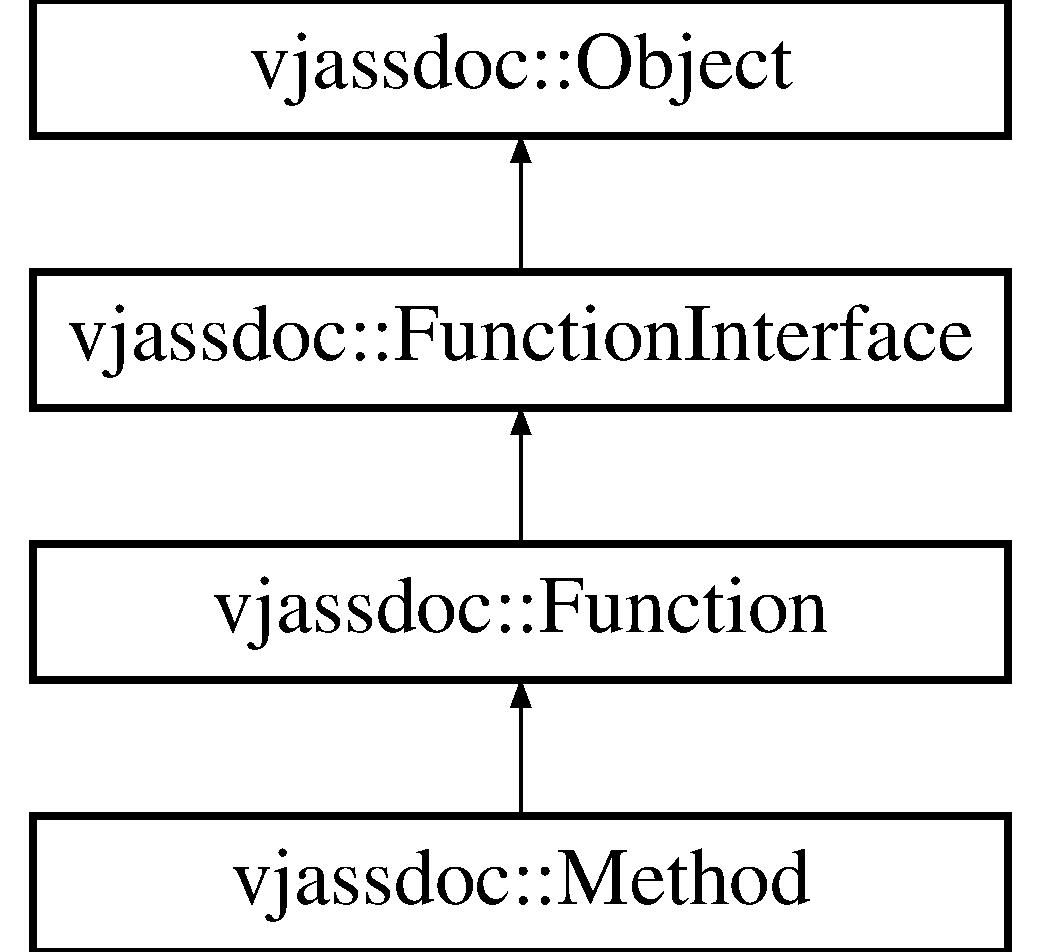
\includegraphics[height=4cm]{classvjassdoc_1_1Function}
\end{center}
\end{figure}
\subsection*{Public Member Functions}
\begin{CompactItemize}
\item 
\hyperlink{classvjassdoc_1_1Function_3505663616782b94aa01a36b789a101b}{Function} (const std::string \&identifier, class \hyperlink{classvjassdoc_1_1SourceFile}{SourceFile} $\ast$sourceFile, unsigned int line, class \hyperlink{classvjassdoc_1_1DocComment}{DocComment} $\ast$docComment, class \hyperlink{classvjassdoc_1_1Library}{Library} $\ast$library, class \hyperlink{classvjassdoc_1_1Scope}{Scope} $\ast$scope, bool isPrivate, std::list$<$ std::string $>$ $\ast$parameterTypeExpressions, std::list$<$ std::string $>$ $\ast$parameters, const std::string \&returnTypeExpression, bool isPublic, bool isConstant, bool isNative)
\item 
\hyperlink{classvjassdoc_1_1Function_3afaafa500bcad415988b9882528b0a7}{Function} (std::vector$<$ const unsigned char $\ast$ $>$ \&columnVector)
\item 
virtual void \hyperlink{classvjassdoc_1_1Function_031d74f7df7c29afb36626fd335b2037}{init} ()
\item 
virtual void \hyperlink{classvjassdoc_1_1Function_b0776a1e111d7fcefbbcecd92f210a48}{pageNavigation} (std::ofstream \&file) const 
\item 
virtual void \hyperlink{classvjassdoc_1_1Function_7f32865b4c3f9f4c4e6379a437f5bdfe}{page} (std::ofstream \&file) const 
\item 
virtual std::string \hyperlink{classvjassdoc_1_1Function_7e4a84e1bb86ade42e6a95d81d8092a7}{sqlStatement} () const 
\item 
bool \hyperlink{classvjassdoc_1_1Function_a8a4c34f800506e7803f875a831014b9}{isPublic} () const 
\item 
bool \hyperlink{classvjassdoc_1_1Function_d94c62d16b874437ed1bb59958f79063}{isConstant} () const 
\item 
bool \hyperlink{classvjassdoc_1_1Function_a4100d5c17d58de39de87648566f5d8b}{isNative} () const 
\end{CompactItemize}


\subsection{Constructor \& Destructor Documentation}
\hypertarget{classvjassdoc_1_1Function_3505663616782b94aa01a36b789a101b}{
\index{vjassdoc::Function@{vjassdoc::Function}!Function@{Function}}
\index{Function@{Function}!vjassdoc::Function@{vjassdoc::Function}}
\subsubsection{\setlength{\rightskip}{0pt plus 5cm}vjassdoc::Function::Function (const std::string \& {\em identifier}, class {\bf SourceFile} $\ast$ {\em sourceFile}, unsigned int {\em line}, class {\bf DocComment} $\ast$ {\em docComment}, class {\bf Library} $\ast$ {\em library}, class {\bf Scope} $\ast$ {\em scope}, bool {\em isPrivate}, std::list$<$ std::string $>$ $\ast$ {\em parameterTypeExpressions}, std::list$<$ std::string $>$ $\ast$ {\em parameters}, const std::string \& {\em returnTypeExpression}, bool {\em isPublic}, bool {\em isConstant}, bool {\em isNative})}}
\label{classvjassdoc_1_1Function_3505663616782b94aa01a36b789a101b}


\hypertarget{classvjassdoc_1_1Function_3afaafa500bcad415988b9882528b0a7}{
\index{vjassdoc::Function@{vjassdoc::Function}!Function@{Function}}
\index{Function@{Function}!vjassdoc::Function@{vjassdoc::Function}}
\subsubsection{\setlength{\rightskip}{0pt plus 5cm}vjassdoc::Function::Function (std::vector$<$ const unsigned char $\ast$ $>$ \& {\em columnVector})}}
\label{classvjassdoc_1_1Function_3afaafa500bcad415988b9882528b0a7}




\subsection{Member Function Documentation}
\hypertarget{classvjassdoc_1_1Function_031d74f7df7c29afb36626fd335b2037}{
\index{vjassdoc::Function@{vjassdoc::Function}!init@{init}}
\index{init@{init}!vjassdoc::Function@{vjassdoc::Function}}
\subsubsection{\setlength{\rightskip}{0pt plus 5cm}void vjassdoc::Function::init ()\hspace{0.3cm}{\tt  \mbox{[}virtual\mbox{]}}}}
\label{classvjassdoc_1_1Function_031d74f7df7c29afb36626fd335b2037}




Reimplemented from \hyperlink{classvjassdoc_1_1FunctionInterface_3b988163d8012beac222b27f80484242}{vjassdoc::FunctionInterface}.

Reimplemented in \hyperlink{classvjassdoc_1_1Method_cd115b1b9a459752e6613925be8e9daf}{vjassdoc::Method}.\hypertarget{classvjassdoc_1_1Function_b0776a1e111d7fcefbbcecd92f210a48}{
\index{vjassdoc::Function@{vjassdoc::Function}!pageNavigation@{pageNavigation}}
\index{pageNavigation@{pageNavigation}!vjassdoc::Function@{vjassdoc::Function}}
\subsubsection{\setlength{\rightskip}{0pt plus 5cm}void vjassdoc::Function::pageNavigation (std::ofstream \& {\em file}) const\hspace{0.3cm}{\tt  \mbox{[}virtual\mbox{]}}}}
\label{classvjassdoc_1_1Function_b0776a1e111d7fcefbbcecd92f210a48}




Reimplemented from \hyperlink{classvjassdoc_1_1FunctionInterface_90bd64ed95596db63699df15aa35216e}{vjassdoc::FunctionInterface}.

Reimplemented in \hyperlink{classvjassdoc_1_1Method_d5d61124a7d28d7e4680cc0df6cc5deb}{vjassdoc::Method}.\hypertarget{classvjassdoc_1_1Function_7f32865b4c3f9f4c4e6379a437f5bdfe}{
\index{vjassdoc::Function@{vjassdoc::Function}!page@{page}}
\index{page@{page}!vjassdoc::Function@{vjassdoc::Function}}
\subsubsection{\setlength{\rightskip}{0pt plus 5cm}void vjassdoc::Function::page (std::ofstream \& {\em file}) const\hspace{0.3cm}{\tt  \mbox{[}virtual\mbox{]}}}}
\label{classvjassdoc_1_1Function_7f32865b4c3f9f4c4e6379a437f5bdfe}




Reimplemented from \hyperlink{classvjassdoc_1_1FunctionInterface_3f5c67bb77822e08047b327f244ec364}{vjassdoc::FunctionInterface}.

Reimplemented in \hyperlink{classvjassdoc_1_1Method_564b24f8b05185ac9399dd36a9b0ad1a}{vjassdoc::Method}.\hypertarget{classvjassdoc_1_1Function_7e4a84e1bb86ade42e6a95d81d8092a7}{
\index{vjassdoc::Function@{vjassdoc::Function}!sqlStatement@{sqlStatement}}
\index{sqlStatement@{sqlStatement}!vjassdoc::Function@{vjassdoc::Function}}
\subsubsection{\setlength{\rightskip}{0pt plus 5cm}std::string vjassdoc::Function::sqlStatement () const\hspace{0.3cm}{\tt  \mbox{[}virtual\mbox{]}}}}
\label{classvjassdoc_1_1Function_7e4a84e1bb86ade42e6a95d81d8092a7}




Reimplemented from \hyperlink{classvjassdoc_1_1FunctionInterface_20b33401bc90587128da6bae1c6986d8}{vjassdoc::FunctionInterface}.

Reimplemented in \hyperlink{classvjassdoc_1_1Method_0a9c4b3b9cb2043eb1454ae72bbfe04f}{vjassdoc::Method}.\hypertarget{classvjassdoc_1_1Function_a8a4c34f800506e7803f875a831014b9}{
\index{vjassdoc::Function@{vjassdoc::Function}!isPublic@{isPublic}}
\index{isPublic@{isPublic}!vjassdoc::Function@{vjassdoc::Function}}
\subsubsection{\setlength{\rightskip}{0pt plus 5cm}bool vjassdoc::Function::isPublic () const\hspace{0.3cm}{\tt  \mbox{[}inline\mbox{]}}}}
\label{classvjassdoc_1_1Function_a8a4c34f800506e7803f875a831014b9}


\hypertarget{classvjassdoc_1_1Function_d94c62d16b874437ed1bb59958f79063}{
\index{vjassdoc::Function@{vjassdoc::Function}!isConstant@{isConstant}}
\index{isConstant@{isConstant}!vjassdoc::Function@{vjassdoc::Function}}
\subsubsection{\setlength{\rightskip}{0pt plus 5cm}bool vjassdoc::Function::isConstant () const\hspace{0.3cm}{\tt  \mbox{[}inline\mbox{]}}}}
\label{classvjassdoc_1_1Function_d94c62d16b874437ed1bb59958f79063}


\hypertarget{classvjassdoc_1_1Function_a4100d5c17d58de39de87648566f5d8b}{
\index{vjassdoc::Function@{vjassdoc::Function}!isNative@{isNative}}
\index{isNative@{isNative}!vjassdoc::Function@{vjassdoc::Function}}
\subsubsection{\setlength{\rightskip}{0pt plus 5cm}bool vjassdoc::Function::isNative () const\hspace{0.3cm}{\tt  \mbox{[}inline\mbox{]}}}}
\label{classvjassdoc_1_1Function_a4100d5c17d58de39de87648566f5d8b}




The documentation for this class was generated from the following files:\begin{CompactItemize}
\item 
src/\hyperlink{function_8h}{function.h}\item 
src/\hyperlink{function_8cpp}{function.cpp}\end{CompactItemize}

\hypertarget{classvjassdoc_1_1FunctionInterface}{
\section{vjassdoc::FunctionInterface Class Reference}
\label{classvjassdoc_1_1FunctionInterface}\index{vjassdoc::FunctionInterface@{vjassdoc::FunctionInterface}}
}
{\tt \#include $<$functioninterface.h$>$}

Inheritance diagram for vjassdoc::FunctionInterface::\begin{figure}[H]
\begin{center}
\leavevmode
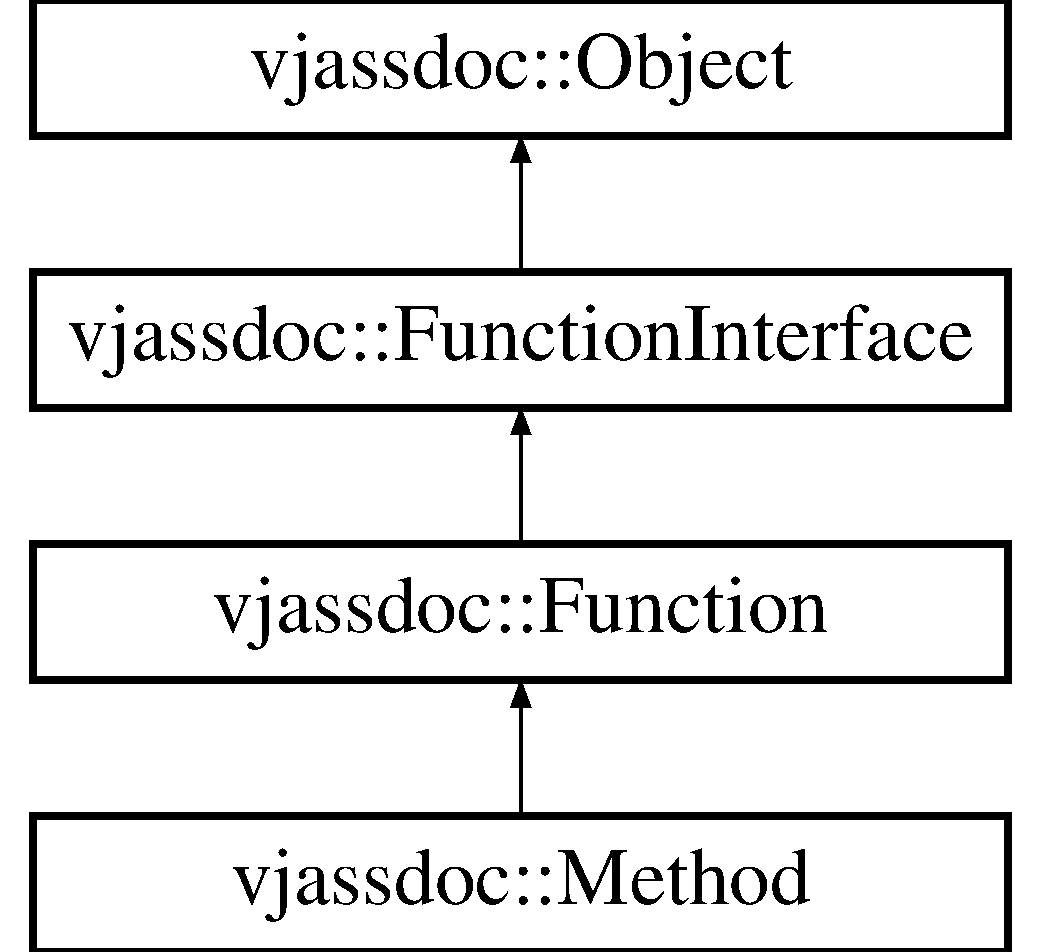
\includegraphics[height=4cm]{classvjassdoc_1_1FunctionInterface}
\end{center}
\end{figure}
\subsection*{Public Member Functions}
\begin{CompactItemize}
\item 
\hyperlink{classvjassdoc_1_1FunctionInterface_0cfa512a726b2d035b42f783d02d6b63}{FunctionInterface} (const std::string \&identifier, class \hyperlink{classvjassdoc_1_1SourceFile}{SourceFile} $\ast$sourceFile, unsigned int line, class \hyperlink{classvjassdoc_1_1DocComment}{DocComment} $\ast$docComment, class \hyperlink{classvjassdoc_1_1Library}{Library} $\ast$library, class \hyperlink{classvjassdoc_1_1Scope}{Scope} $\ast$scope, bool isPrivate, std::list$<$ std::string $>$ $\ast$parameterTypeExpressions, std::list$<$ std::string $>$ $\ast$parameters, const std::string \&returnTypeExpression)
\item 
\hyperlink{classvjassdoc_1_1FunctionInterface_0eae365567f49506b31b3f8c860550f2}{FunctionInterface} (std::vector$<$ const unsigned char $\ast$ $>$ \&columnVector)
\item 
virtual \hyperlink{classvjassdoc_1_1FunctionInterface_35cab1ce58b14423de2f6c183f1ba9d8}{$\sim$FunctionInterface} ()
\item 
virtual void \hyperlink{classvjassdoc_1_1FunctionInterface_3b988163d8012beac222b27f80484242}{init} ()
\item 
virtual void \hyperlink{classvjassdoc_1_1FunctionInterface_90bd64ed95596db63699df15aa35216e}{pageNavigation} (std::ofstream \&file) const 
\item 
virtual void \hyperlink{classvjassdoc_1_1FunctionInterface_3f5c67bb77822e08047b327f244ec364}{page} (std::ofstream \&file) const 
\item 
virtual std::string \hyperlink{classvjassdoc_1_1FunctionInterface_20b33401bc90587128da6bae1c6986d8}{sqlStatement} () const 
\item 
virtual class \hyperlink{classvjassdoc_1_1Library}{Library} $\ast$ \hyperlink{classvjassdoc_1_1FunctionInterface_c9519495c94b07101fa5e0739775759e}{library} () const 
\item 
virtual class \hyperlink{classvjassdoc_1_1Scope}{Scope} $\ast$ \hyperlink{classvjassdoc_1_1FunctionInterface_3d298257fab6e122f44f07225ee3ab63}{scope} () const 
\item 
bool \hyperlink{classvjassdoc_1_1FunctionInterface_8b81d3aee374ba63043fcc06ec2eec1e}{isPrivate} () const 
\item 
std::list$<$ class \hyperlink{classvjassdoc_1_1Object}{Object} $\ast$ $>$ $\ast$ \hyperlink{classvjassdoc_1_1FunctionInterface_fee3dfa7efa4bf0d40b27155cdfa3089}{parameterTypes} () const 
\item 
std::list$<$ std::string $>$ $\ast$ \hyperlink{classvjassdoc_1_1FunctionInterface_5a4199aa5d1aae02b27bb41d76e2dc70}{parameterTypeExpressions} () const 
\item 
std::list$<$ std::string $>$ $\ast$ \hyperlink{classvjassdoc_1_1FunctionInterface_93f6d443529b9f3bb2f9ed679b4dc97a}{parameters} () const 
\item 
class \hyperlink{classvjassdoc_1_1Object}{Object} $\ast$ \hyperlink{classvjassdoc_1_1FunctionInterface_5ad6508146fcb9e7c8accf22a0e4d563}{returnType} () const 
\item 
std::string \hyperlink{classvjassdoc_1_1FunctionInterface_951b692881136d487bb89b1dce203f08}{returnTypeExpression} () const 
\end{CompactItemize}


\subsection{Constructor \& Destructor Documentation}
\hypertarget{classvjassdoc_1_1FunctionInterface_0cfa512a726b2d035b42f783d02d6b63}{
\index{vjassdoc::FunctionInterface@{vjassdoc::FunctionInterface}!FunctionInterface@{FunctionInterface}}
\index{FunctionInterface@{FunctionInterface}!vjassdoc::FunctionInterface@{vjassdoc::FunctionInterface}}
\subsubsection{\setlength{\rightskip}{0pt plus 5cm}vjassdoc::FunctionInterface::FunctionInterface (const std::string \& {\em identifier}, class {\bf SourceFile} $\ast$ {\em sourceFile}, unsigned int {\em line}, class {\bf DocComment} $\ast$ {\em docComment}, class {\bf Library} $\ast$ {\em library}, class {\bf Scope} $\ast$ {\em scope}, bool {\em isPrivate}, std::list$<$ std::string $>$ $\ast$ {\em parameterTypeExpressions}, std::list$<$ std::string $>$ $\ast$ {\em parameters}, const std::string \& {\em returnTypeExpression})}}
\label{classvjassdoc_1_1FunctionInterface_0cfa512a726b2d035b42f783d02d6b63}


\hypertarget{classvjassdoc_1_1FunctionInterface_0eae365567f49506b31b3f8c860550f2}{
\index{vjassdoc::FunctionInterface@{vjassdoc::FunctionInterface}!FunctionInterface@{FunctionInterface}}
\index{FunctionInterface@{FunctionInterface}!vjassdoc::FunctionInterface@{vjassdoc::FunctionInterface}}
\subsubsection{\setlength{\rightskip}{0pt plus 5cm}vjassdoc::FunctionInterface::FunctionInterface (std::vector$<$ const unsigned char $\ast$ $>$ \& {\em columnVector})}}
\label{classvjassdoc_1_1FunctionInterface_0eae365567f49506b31b3f8c860550f2}


\hypertarget{classvjassdoc_1_1FunctionInterface_35cab1ce58b14423de2f6c183f1ba9d8}{
\index{vjassdoc::FunctionInterface@{vjassdoc::FunctionInterface}!$\sim$FunctionInterface@{$\sim$FunctionInterface}}
\index{$\sim$FunctionInterface@{$\sim$FunctionInterface}!vjassdoc::FunctionInterface@{vjassdoc::FunctionInterface}}
\subsubsection{\setlength{\rightskip}{0pt plus 5cm}vjassdoc::FunctionInterface::$\sim$FunctionInterface ()\hspace{0.3cm}{\tt  \mbox{[}virtual\mbox{]}}}}
\label{classvjassdoc_1_1FunctionInterface_35cab1ce58b14423de2f6c183f1ba9d8}




\subsection{Member Function Documentation}
\hypertarget{classvjassdoc_1_1FunctionInterface_3b988163d8012beac222b27f80484242}{
\index{vjassdoc::FunctionInterface@{vjassdoc::FunctionInterface}!init@{init}}
\index{init@{init}!vjassdoc::FunctionInterface@{vjassdoc::FunctionInterface}}
\subsubsection{\setlength{\rightskip}{0pt plus 5cm}void vjassdoc::FunctionInterface::init ()\hspace{0.3cm}{\tt  \mbox{[}virtual\mbox{]}}}}
\label{classvjassdoc_1_1FunctionInterface_3b988163d8012beac222b27f80484242}




Implements \hyperlink{classvjassdoc_1_1Object_bd43e77dbe80055f5adda67661dfaca4}{vjassdoc::Object}.

Reimplemented in \hyperlink{classvjassdoc_1_1Function_031d74f7df7c29afb36626fd335b2037}{vjassdoc::Function}, and \hyperlink{classvjassdoc_1_1Method_cd115b1b9a459752e6613925be8e9daf}{vjassdoc::Method}.\hypertarget{classvjassdoc_1_1FunctionInterface_90bd64ed95596db63699df15aa35216e}{
\index{vjassdoc::FunctionInterface@{vjassdoc::FunctionInterface}!pageNavigation@{pageNavigation}}
\index{pageNavigation@{pageNavigation}!vjassdoc::FunctionInterface@{vjassdoc::FunctionInterface}}
\subsubsection{\setlength{\rightskip}{0pt plus 5cm}void vjassdoc::FunctionInterface::pageNavigation (std::ofstream \& {\em file}) const\hspace{0.3cm}{\tt  \mbox{[}virtual\mbox{]}}}}
\label{classvjassdoc_1_1FunctionInterface_90bd64ed95596db63699df15aa35216e}




Implements \hyperlink{classvjassdoc_1_1Object_736bbb6719edd8070d8f56c364a2764c}{vjassdoc::Object}.

Reimplemented in \hyperlink{classvjassdoc_1_1Function_b0776a1e111d7fcefbbcecd92f210a48}{vjassdoc::Function}, and \hyperlink{classvjassdoc_1_1Method_d5d61124a7d28d7e4680cc0df6cc5deb}{vjassdoc::Method}.\hypertarget{classvjassdoc_1_1FunctionInterface_3f5c67bb77822e08047b327f244ec364}{
\index{vjassdoc::FunctionInterface@{vjassdoc::FunctionInterface}!page@{page}}
\index{page@{page}!vjassdoc::FunctionInterface@{vjassdoc::FunctionInterface}}
\subsubsection{\setlength{\rightskip}{0pt plus 5cm}void vjassdoc::FunctionInterface::page (std::ofstream \& {\em file}) const\hspace{0.3cm}{\tt  \mbox{[}virtual\mbox{]}}}}
\label{classvjassdoc_1_1FunctionInterface_3f5c67bb77822e08047b327f244ec364}




Implements \hyperlink{classvjassdoc_1_1Object_a0489e38956f3507566b1bc6e3e2c8af}{vjassdoc::Object}.

Reimplemented in \hyperlink{classvjassdoc_1_1Function_7f32865b4c3f9f4c4e6379a437f5bdfe}{vjassdoc::Function}, and \hyperlink{classvjassdoc_1_1Method_564b24f8b05185ac9399dd36a9b0ad1a}{vjassdoc::Method}.\hypertarget{classvjassdoc_1_1FunctionInterface_20b33401bc90587128da6bae1c6986d8}{
\index{vjassdoc::FunctionInterface@{vjassdoc::FunctionInterface}!sqlStatement@{sqlStatement}}
\index{sqlStatement@{sqlStatement}!vjassdoc::FunctionInterface@{vjassdoc::FunctionInterface}}
\subsubsection{\setlength{\rightskip}{0pt plus 5cm}std::string vjassdoc::FunctionInterface::sqlStatement () const\hspace{0.3cm}{\tt  \mbox{[}virtual\mbox{]}}}}
\label{classvjassdoc_1_1FunctionInterface_20b33401bc90587128da6bae1c6986d8}




Reimplemented from \hyperlink{classvjassdoc_1_1Object_4e8ebbb0ce5b0bf91ec847b1e4a9f8fc}{vjassdoc::Object}.

Reimplemented in \hyperlink{classvjassdoc_1_1Function_7e4a84e1bb86ade42e6a95d81d8092a7}{vjassdoc::Function}, and \hyperlink{classvjassdoc_1_1Method_0a9c4b3b9cb2043eb1454ae72bbfe04f}{vjassdoc::Method}.\hypertarget{classvjassdoc_1_1FunctionInterface_c9519495c94b07101fa5e0739775759e}{
\index{vjassdoc::FunctionInterface@{vjassdoc::FunctionInterface}!library@{library}}
\index{library@{library}!vjassdoc::FunctionInterface@{vjassdoc::FunctionInterface}}
\subsubsection{\setlength{\rightskip}{0pt plus 5cm}class {\bf Library} $\ast$ vjassdoc::FunctionInterface::library () const\hspace{0.3cm}{\tt  \mbox{[}virtual\mbox{]}}}}
\label{classvjassdoc_1_1FunctionInterface_c9519495c94b07101fa5e0739775759e}




Reimplemented from \hyperlink{classvjassdoc_1_1Object_cc4241505c5bcdd0bbcb08a1b665b3fd}{vjassdoc::Object}.\hypertarget{classvjassdoc_1_1FunctionInterface_3d298257fab6e122f44f07225ee3ab63}{
\index{vjassdoc::FunctionInterface@{vjassdoc::FunctionInterface}!scope@{scope}}
\index{scope@{scope}!vjassdoc::FunctionInterface@{vjassdoc::FunctionInterface}}
\subsubsection{\setlength{\rightskip}{0pt plus 5cm}class {\bf Scope} $\ast$ vjassdoc::FunctionInterface::scope () const\hspace{0.3cm}{\tt  \mbox{[}virtual\mbox{]}}}}
\label{classvjassdoc_1_1FunctionInterface_3d298257fab6e122f44f07225ee3ab63}




Reimplemented from \hyperlink{classvjassdoc_1_1Object_0738d05b196cc8b9e89d62839d81fc20}{vjassdoc::Object}.\hypertarget{classvjassdoc_1_1FunctionInterface_8b81d3aee374ba63043fcc06ec2eec1e}{
\index{vjassdoc::FunctionInterface@{vjassdoc::FunctionInterface}!isPrivate@{isPrivate}}
\index{isPrivate@{isPrivate}!vjassdoc::FunctionInterface@{vjassdoc::FunctionInterface}}
\subsubsection{\setlength{\rightskip}{0pt plus 5cm}bool vjassdoc::FunctionInterface::isPrivate () const\hspace{0.3cm}{\tt  \mbox{[}inline\mbox{]}}}}
\label{classvjassdoc_1_1FunctionInterface_8b81d3aee374ba63043fcc06ec2eec1e}


\hypertarget{classvjassdoc_1_1FunctionInterface_fee3dfa7efa4bf0d40b27155cdfa3089}{
\index{vjassdoc::FunctionInterface@{vjassdoc::FunctionInterface}!parameterTypes@{parameterTypes}}
\index{parameterTypes@{parameterTypes}!vjassdoc::FunctionInterface@{vjassdoc::FunctionInterface}}
\subsubsection{\setlength{\rightskip}{0pt plus 5cm}std::list$<$ class {\bf Object} $\ast$ $>$ $\ast$ vjassdoc::FunctionInterface::parameterTypes () const\hspace{0.3cm}{\tt  \mbox{[}inline\mbox{]}}}}
\label{classvjassdoc_1_1FunctionInterface_fee3dfa7efa4bf0d40b27155cdfa3089}


\hypertarget{classvjassdoc_1_1FunctionInterface_5a4199aa5d1aae02b27bb41d76e2dc70}{
\index{vjassdoc::FunctionInterface@{vjassdoc::FunctionInterface}!parameterTypeExpressions@{parameterTypeExpressions}}
\index{parameterTypeExpressions@{parameterTypeExpressions}!vjassdoc::FunctionInterface@{vjassdoc::FunctionInterface}}
\subsubsection{\setlength{\rightskip}{0pt plus 5cm}std::list$<$ std::string $>$ $\ast$ vjassdoc::FunctionInterface::parameterTypeExpressions () const\hspace{0.3cm}{\tt  \mbox{[}inline\mbox{]}}}}
\label{classvjassdoc_1_1FunctionInterface_5a4199aa5d1aae02b27bb41d76e2dc70}


\hypertarget{classvjassdoc_1_1FunctionInterface_93f6d443529b9f3bb2f9ed679b4dc97a}{
\index{vjassdoc::FunctionInterface@{vjassdoc::FunctionInterface}!parameters@{parameters}}
\index{parameters@{parameters}!vjassdoc::FunctionInterface@{vjassdoc::FunctionInterface}}
\subsubsection{\setlength{\rightskip}{0pt plus 5cm}std::list$<$ std::string $>$ $\ast$ vjassdoc::FunctionInterface::parameters () const\hspace{0.3cm}{\tt  \mbox{[}inline\mbox{]}}}}
\label{classvjassdoc_1_1FunctionInterface_93f6d443529b9f3bb2f9ed679b4dc97a}


\hypertarget{classvjassdoc_1_1FunctionInterface_5ad6508146fcb9e7c8accf22a0e4d563}{
\index{vjassdoc::FunctionInterface@{vjassdoc::FunctionInterface}!returnType@{returnType}}
\index{returnType@{returnType}!vjassdoc::FunctionInterface@{vjassdoc::FunctionInterface}}
\subsubsection{\setlength{\rightskip}{0pt plus 5cm}class {\bf Object} $\ast$ vjassdoc::FunctionInterface::returnType () const\hspace{0.3cm}{\tt  \mbox{[}inline\mbox{]}}}}
\label{classvjassdoc_1_1FunctionInterface_5ad6508146fcb9e7c8accf22a0e4d563}


\hypertarget{classvjassdoc_1_1FunctionInterface_951b692881136d487bb89b1dce203f08}{
\index{vjassdoc::FunctionInterface@{vjassdoc::FunctionInterface}!returnTypeExpression@{returnTypeExpression}}
\index{returnTypeExpression@{returnTypeExpression}!vjassdoc::FunctionInterface@{vjassdoc::FunctionInterface}}
\subsubsection{\setlength{\rightskip}{0pt plus 5cm}std::string vjassdoc::FunctionInterface::returnTypeExpression () const\hspace{0.3cm}{\tt  \mbox{[}inline\mbox{]}}}}
\label{classvjassdoc_1_1FunctionInterface_951b692881136d487bb89b1dce203f08}




The documentation for this class was generated from the following files:\begin{CompactItemize}
\item 
src/\hyperlink{functioninterface_8h}{functioninterface.h}\item 
src/\hyperlink{functioninterface_8cpp}{functioninterface.cpp}\end{CompactItemize}

\hypertarget{classvjassdoc_1_1Global}{
\section{vjassdoc::Global Class Reference}
\label{classvjassdoc_1_1Global}\index{vjassdoc::Global@{vjassdoc::Global}}
}
{\tt \#include $<$global.h$>$}

Inheritance diagram for vjassdoc::Global::\begin{figure}[H]
\begin{center}
\leavevmode
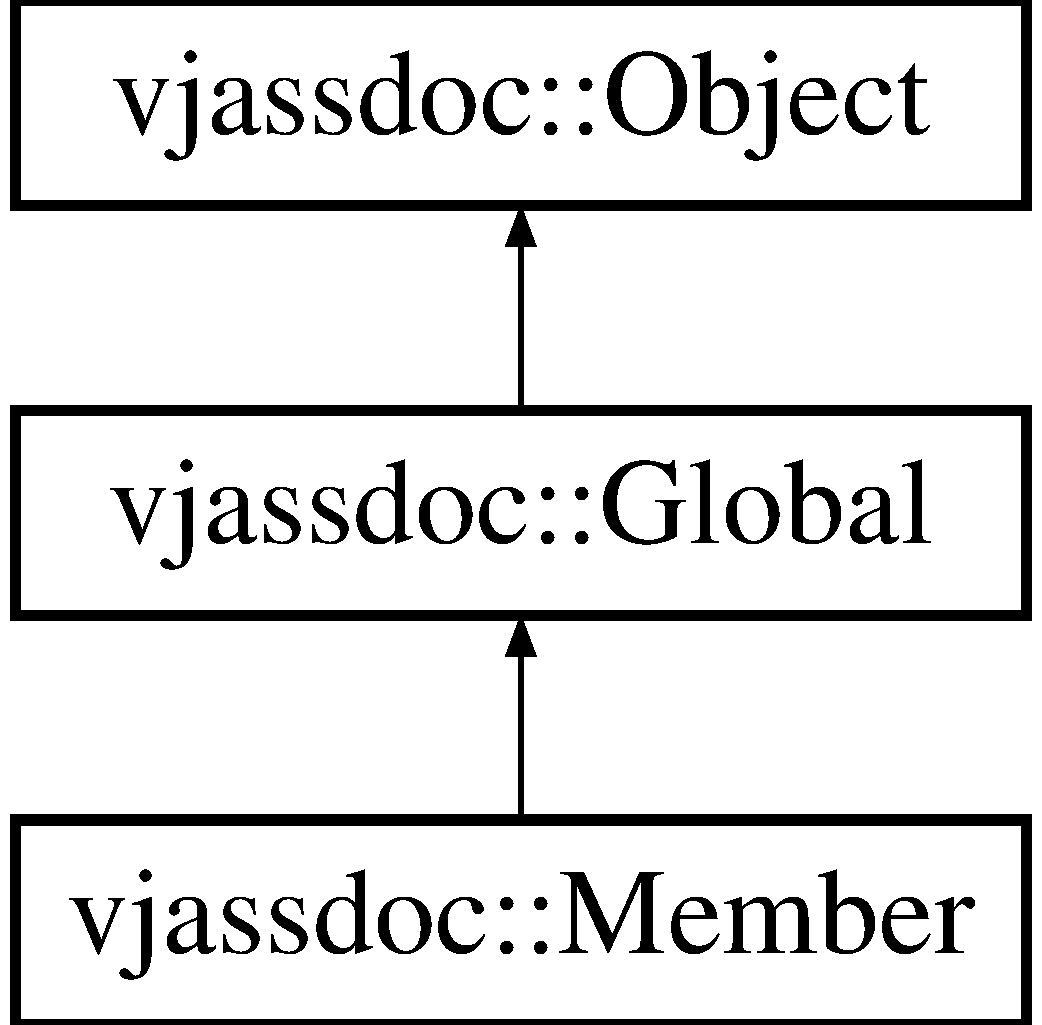
\includegraphics[height=3cm]{classvjassdoc_1_1Global}
\end{center}
\end{figure}
\subsection*{Public Member Functions}
\begin{CompactItemize}
\item 
\hyperlink{classvjassdoc_1_1Global_9914271ade5a5e8cd9261a29cbbb9516}{Global} (const std::string \&identifier, class \hyperlink{classvjassdoc_1_1SourceFile}{SourceFile} $\ast$sourceFile, unsigned int line, class \hyperlink{classvjassdoc_1_1DocComment}{DocComment} $\ast$docComment, class \hyperlink{classvjassdoc_1_1Library}{Library} $\ast$library, class \hyperlink{classvjassdoc_1_1Scope}{Scope} $\ast$scope, bool isPrivate, bool isPublic, bool isConstant, const std::string \&typeExpression, const std::string \&valueExpression, const std::string \&sizeExpression)
\item 
\hyperlink{classvjassdoc_1_1Global_4b22573ef7ba055be457713685a7b067}{Global} (std::vector$<$ const unsigned char $\ast$ $>$ \&columnVector)
\item 
virtual void \hyperlink{classvjassdoc_1_1Global_9e6189cfd577f0453988e8c8c6eec04d}{init} ()
\item 
virtual void \hyperlink{classvjassdoc_1_1Global_8c5209b5652d3633feb1d7fab796b439}{pageNavigation} (std::ofstream \&file) const 
\item 
virtual void \hyperlink{classvjassdoc_1_1Global_1b8fefe2b9c895c122a822bac0383f1b}{page} (std::ofstream \&file) const 
\item 
virtual std::string \hyperlink{classvjassdoc_1_1Global_4e9a8ea0c8bc34f6980d31676e497531}{sqlStatement} () const 
\item 
virtual class \hyperlink{classvjassdoc_1_1Library}{Library} $\ast$ \hyperlink{classvjassdoc_1_1Global_cbf7be8310f31bd7dc142b290020b4a9}{library} () const 
\item 
virtual class \hyperlink{classvjassdoc_1_1Scope}{Scope} $\ast$ \hyperlink{classvjassdoc_1_1Global_239f8dbfff5e8ed7580d6ba9aadd5f55}{scope} () const 
\item 
bool \hyperlink{classvjassdoc_1_1Global_58459a301561ab4f9995d303365176b2}{isPrivate} () const 
\item 
bool \hyperlink{classvjassdoc_1_1Global_0294eb0932bb61f8fbca0d96d6a478a5}{isPublic} () const 
\item 
bool \hyperlink{classvjassdoc_1_1Global_cbefeff067aa589f960f261991d4213a}{isConstant} () const 
\item 
class \hyperlink{classvjassdoc_1_1Object}{Object} $\ast$ \hyperlink{classvjassdoc_1_1Global_79c4a6767d7e87b7429386f106082f96}{type} () const 
\item 
std::string \hyperlink{classvjassdoc_1_1Global_fd1b0ad435dae30a0e44f472baf11b25}{typeExpression} () const 
\item 
class \hyperlink{classvjassdoc_1_1Object}{Object} $\ast$ \hyperlink{classvjassdoc_1_1Global_1dd411e17e0b5090990571d73459e2a5}{value} () const 
\item 
std::string \hyperlink{classvjassdoc_1_1Global_9306c48075e65d76a8324959006ffebb}{valueLiteral} () const 
\item 
class \hyperlink{classvjassdoc_1_1Object}{Object} $\ast$ \hyperlink{classvjassdoc_1_1Global_e3ad49253eccec78bd93e7bd12494303}{size} () const 
\item 
int \hyperlink{classvjassdoc_1_1Global_2029ac82912ebe23066c48e13ab2b1a2}{sizeLiteral} () const 
\end{CompactItemize}


\subsection{Constructor \& Destructor Documentation}
\hypertarget{classvjassdoc_1_1Global_9914271ade5a5e8cd9261a29cbbb9516}{
\index{vjassdoc::Global@{vjassdoc::Global}!Global@{Global}}
\index{Global@{Global}!vjassdoc::Global@{vjassdoc::Global}}
\subsubsection{\setlength{\rightskip}{0pt plus 5cm}vjassdoc::Global::Global (const std::string \& {\em identifier}, class {\bf SourceFile} $\ast$ {\em sourceFile}, unsigned int {\em line}, class {\bf DocComment} $\ast$ {\em docComment}, class {\bf Library} $\ast$ {\em library}, class {\bf Scope} $\ast$ {\em scope}, bool {\em isPrivate}, bool {\em isPublic}, bool {\em isConstant}, const std::string \& {\em typeExpression}, const std::string \& {\em valueExpression}, const std::string \& {\em sizeExpression})}}
\label{classvjassdoc_1_1Global_9914271ade5a5e8cd9261a29cbbb9516}


\hypertarget{classvjassdoc_1_1Global_4b22573ef7ba055be457713685a7b067}{
\index{vjassdoc::Global@{vjassdoc::Global}!Global@{Global}}
\index{Global@{Global}!vjassdoc::Global@{vjassdoc::Global}}
\subsubsection{\setlength{\rightskip}{0pt plus 5cm}vjassdoc::Global::Global (std::vector$<$ const unsigned char $\ast$ $>$ \& {\em columnVector})}}
\label{classvjassdoc_1_1Global_4b22573ef7ba055be457713685a7b067}




\subsection{Member Function Documentation}
\hypertarget{classvjassdoc_1_1Global_9e6189cfd577f0453988e8c8c6eec04d}{
\index{vjassdoc::Global@{vjassdoc::Global}!init@{init}}
\index{init@{init}!vjassdoc::Global@{vjassdoc::Global}}
\subsubsection{\setlength{\rightskip}{0pt plus 5cm}void vjassdoc::Global::init ()\hspace{0.3cm}{\tt  \mbox{[}virtual\mbox{]}}}}
\label{classvjassdoc_1_1Global_9e6189cfd577f0453988e8c8c6eec04d}




Implements \hyperlink{classvjassdoc_1_1Object_bd43e77dbe80055f5adda67661dfaca4}{vjassdoc::Object}.

Reimplemented in \hyperlink{classvjassdoc_1_1Member_eccac74ca5ea37e82d322c20b5aa2efc}{vjassdoc::Member}.\hypertarget{classvjassdoc_1_1Global_8c5209b5652d3633feb1d7fab796b439}{
\index{vjassdoc::Global@{vjassdoc::Global}!pageNavigation@{pageNavigation}}
\index{pageNavigation@{pageNavigation}!vjassdoc::Global@{vjassdoc::Global}}
\subsubsection{\setlength{\rightskip}{0pt plus 5cm}void vjassdoc::Global::pageNavigation (std::ofstream \& {\em file}) const\hspace{0.3cm}{\tt  \mbox{[}virtual\mbox{]}}}}
\label{classvjassdoc_1_1Global_8c5209b5652d3633feb1d7fab796b439}




Implements \hyperlink{classvjassdoc_1_1Object_736bbb6719edd8070d8f56c364a2764c}{vjassdoc::Object}.

Reimplemented in \hyperlink{classvjassdoc_1_1Member_fa8e020175714b1f03a3696cc935941f}{vjassdoc::Member}.\hypertarget{classvjassdoc_1_1Global_1b8fefe2b9c895c122a822bac0383f1b}{
\index{vjassdoc::Global@{vjassdoc::Global}!page@{page}}
\index{page@{page}!vjassdoc::Global@{vjassdoc::Global}}
\subsubsection{\setlength{\rightskip}{0pt plus 5cm}void vjassdoc::Global::page (std::ofstream \& {\em file}) const\hspace{0.3cm}{\tt  \mbox{[}virtual\mbox{]}}}}
\label{classvjassdoc_1_1Global_1b8fefe2b9c895c122a822bac0383f1b}




Implements \hyperlink{classvjassdoc_1_1Object_a0489e38956f3507566b1bc6e3e2c8af}{vjassdoc::Object}.

Reimplemented in \hyperlink{classvjassdoc_1_1Member_2bd66eba1882dfb2dcbf2552b42d1346}{vjassdoc::Member}.\hypertarget{classvjassdoc_1_1Global_4e9a8ea0c8bc34f6980d31676e497531}{
\index{vjassdoc::Global@{vjassdoc::Global}!sqlStatement@{sqlStatement}}
\index{sqlStatement@{sqlStatement}!vjassdoc::Global@{vjassdoc::Global}}
\subsubsection{\setlength{\rightskip}{0pt plus 5cm}std::string vjassdoc::Global::sqlStatement () const\hspace{0.3cm}{\tt  \mbox{[}virtual\mbox{]}}}}
\label{classvjassdoc_1_1Global_4e9a8ea0c8bc34f6980d31676e497531}




Reimplemented from \hyperlink{classvjassdoc_1_1Object_4e8ebbb0ce5b0bf91ec847b1e4a9f8fc}{vjassdoc::Object}.

Reimplemented in \hyperlink{classvjassdoc_1_1Member_ad210521f998bd4c8be5f8af3ae74cf1}{vjassdoc::Member}.\hypertarget{classvjassdoc_1_1Global_cbf7be8310f31bd7dc142b290020b4a9}{
\index{vjassdoc::Global@{vjassdoc::Global}!library@{library}}
\index{library@{library}!vjassdoc::Global@{vjassdoc::Global}}
\subsubsection{\setlength{\rightskip}{0pt plus 5cm}class {\bf Library} $\ast$ vjassdoc::Global::library () const\hspace{0.3cm}{\tt  \mbox{[}virtual\mbox{]}}}}
\label{classvjassdoc_1_1Global_cbf7be8310f31bd7dc142b290020b4a9}




Reimplemented from \hyperlink{classvjassdoc_1_1Object_cc4241505c5bcdd0bbcb08a1b665b3fd}{vjassdoc::Object}.\hypertarget{classvjassdoc_1_1Global_239f8dbfff5e8ed7580d6ba9aadd5f55}{
\index{vjassdoc::Global@{vjassdoc::Global}!scope@{scope}}
\index{scope@{scope}!vjassdoc::Global@{vjassdoc::Global}}
\subsubsection{\setlength{\rightskip}{0pt plus 5cm}class {\bf Scope} $\ast$ vjassdoc::Global::scope () const\hspace{0.3cm}{\tt  \mbox{[}virtual\mbox{]}}}}
\label{classvjassdoc_1_1Global_239f8dbfff5e8ed7580d6ba9aadd5f55}




Reimplemented from \hyperlink{classvjassdoc_1_1Object_0738d05b196cc8b9e89d62839d81fc20}{vjassdoc::Object}.\hypertarget{classvjassdoc_1_1Global_58459a301561ab4f9995d303365176b2}{
\index{vjassdoc::Global@{vjassdoc::Global}!isPrivate@{isPrivate}}
\index{isPrivate@{isPrivate}!vjassdoc::Global@{vjassdoc::Global}}
\subsubsection{\setlength{\rightskip}{0pt plus 5cm}bool vjassdoc::Global::isPrivate () const\hspace{0.3cm}{\tt  \mbox{[}inline\mbox{]}}}}
\label{classvjassdoc_1_1Global_58459a301561ab4f9995d303365176b2}


\hypertarget{classvjassdoc_1_1Global_0294eb0932bb61f8fbca0d96d6a478a5}{
\index{vjassdoc::Global@{vjassdoc::Global}!isPublic@{isPublic}}
\index{isPublic@{isPublic}!vjassdoc::Global@{vjassdoc::Global}}
\subsubsection{\setlength{\rightskip}{0pt plus 5cm}bool vjassdoc::Global::isPublic () const\hspace{0.3cm}{\tt  \mbox{[}inline\mbox{]}}}}
\label{classvjassdoc_1_1Global_0294eb0932bb61f8fbca0d96d6a478a5}


\hypertarget{classvjassdoc_1_1Global_cbefeff067aa589f960f261991d4213a}{
\index{vjassdoc::Global@{vjassdoc::Global}!isConstant@{isConstant}}
\index{isConstant@{isConstant}!vjassdoc::Global@{vjassdoc::Global}}
\subsubsection{\setlength{\rightskip}{0pt plus 5cm}bool vjassdoc::Global::isConstant () const\hspace{0.3cm}{\tt  \mbox{[}inline\mbox{]}}}}
\label{classvjassdoc_1_1Global_cbefeff067aa589f960f261991d4213a}


\hypertarget{classvjassdoc_1_1Global_79c4a6767d7e87b7429386f106082f96}{
\index{vjassdoc::Global@{vjassdoc::Global}!type@{type}}
\index{type@{type}!vjassdoc::Global@{vjassdoc::Global}}
\subsubsection{\setlength{\rightskip}{0pt plus 5cm}class {\bf Object} $\ast$ vjassdoc::Global::type () const\hspace{0.3cm}{\tt  \mbox{[}inline\mbox{]}}}}
\label{classvjassdoc_1_1Global_79c4a6767d7e87b7429386f106082f96}


\hypertarget{classvjassdoc_1_1Global_fd1b0ad435dae30a0e44f472baf11b25}{
\index{vjassdoc::Global@{vjassdoc::Global}!typeExpression@{typeExpression}}
\index{typeExpression@{typeExpression}!vjassdoc::Global@{vjassdoc::Global}}
\subsubsection{\setlength{\rightskip}{0pt plus 5cm}std::string vjassdoc::Global::typeExpression () const\hspace{0.3cm}{\tt  \mbox{[}inline\mbox{]}}}}
\label{classvjassdoc_1_1Global_fd1b0ad435dae30a0e44f472baf11b25}


\hypertarget{classvjassdoc_1_1Global_1dd411e17e0b5090990571d73459e2a5}{
\index{vjassdoc::Global@{vjassdoc::Global}!value@{value}}
\index{value@{value}!vjassdoc::Global@{vjassdoc::Global}}
\subsubsection{\setlength{\rightskip}{0pt plus 5cm}class {\bf Object} $\ast$ vjassdoc::Global::value () const\hspace{0.3cm}{\tt  \mbox{[}inline\mbox{]}}}}
\label{classvjassdoc_1_1Global_1dd411e17e0b5090990571d73459e2a5}


\hypertarget{classvjassdoc_1_1Global_9306c48075e65d76a8324959006ffebb}{
\index{vjassdoc::Global@{vjassdoc::Global}!valueLiteral@{valueLiteral}}
\index{valueLiteral@{valueLiteral}!vjassdoc::Global@{vjassdoc::Global}}
\subsubsection{\setlength{\rightskip}{0pt plus 5cm}std::string vjassdoc::Global::valueLiteral () const\hspace{0.3cm}{\tt  \mbox{[}inline\mbox{]}}}}
\label{classvjassdoc_1_1Global_9306c48075e65d76a8324959006ffebb}


\hypertarget{classvjassdoc_1_1Global_e3ad49253eccec78bd93e7bd12494303}{
\index{vjassdoc::Global@{vjassdoc::Global}!size@{size}}
\index{size@{size}!vjassdoc::Global@{vjassdoc::Global}}
\subsubsection{\setlength{\rightskip}{0pt plus 5cm}class {\bf Object} $\ast$ vjassdoc::Global::size () const\hspace{0.3cm}{\tt  \mbox{[}inline\mbox{]}}}}
\label{classvjassdoc_1_1Global_e3ad49253eccec78bd93e7bd12494303}


\hypertarget{classvjassdoc_1_1Global_2029ac82912ebe23066c48e13ab2b1a2}{
\index{vjassdoc::Global@{vjassdoc::Global}!sizeLiteral@{sizeLiteral}}
\index{sizeLiteral@{sizeLiteral}!vjassdoc::Global@{vjassdoc::Global}}
\subsubsection{\setlength{\rightskip}{0pt plus 5cm}int vjassdoc::Global::sizeLiteral () const\hspace{0.3cm}{\tt  \mbox{[}inline\mbox{]}}}}
\label{classvjassdoc_1_1Global_2029ac82912ebe23066c48e13ab2b1a2}




The documentation for this class was generated from the following files:\begin{CompactItemize}
\item 
src/\hyperlink{global_8h}{global.h}\item 
src/\hyperlink{global_8cpp}{global.cpp}\end{CompactItemize}

\hypertarget{classvjassdoc_1_1Interface}{
\section{vjassdoc::Interface Class Reference}
\label{classvjassdoc_1_1Interface}\index{vjassdoc::Interface@{vjassdoc::Interface}}
}
{\tt \#include $<$interface.h$>$}

Inheritance diagram for vjassdoc::Interface::\begin{figure}[H]
\begin{center}
\leavevmode
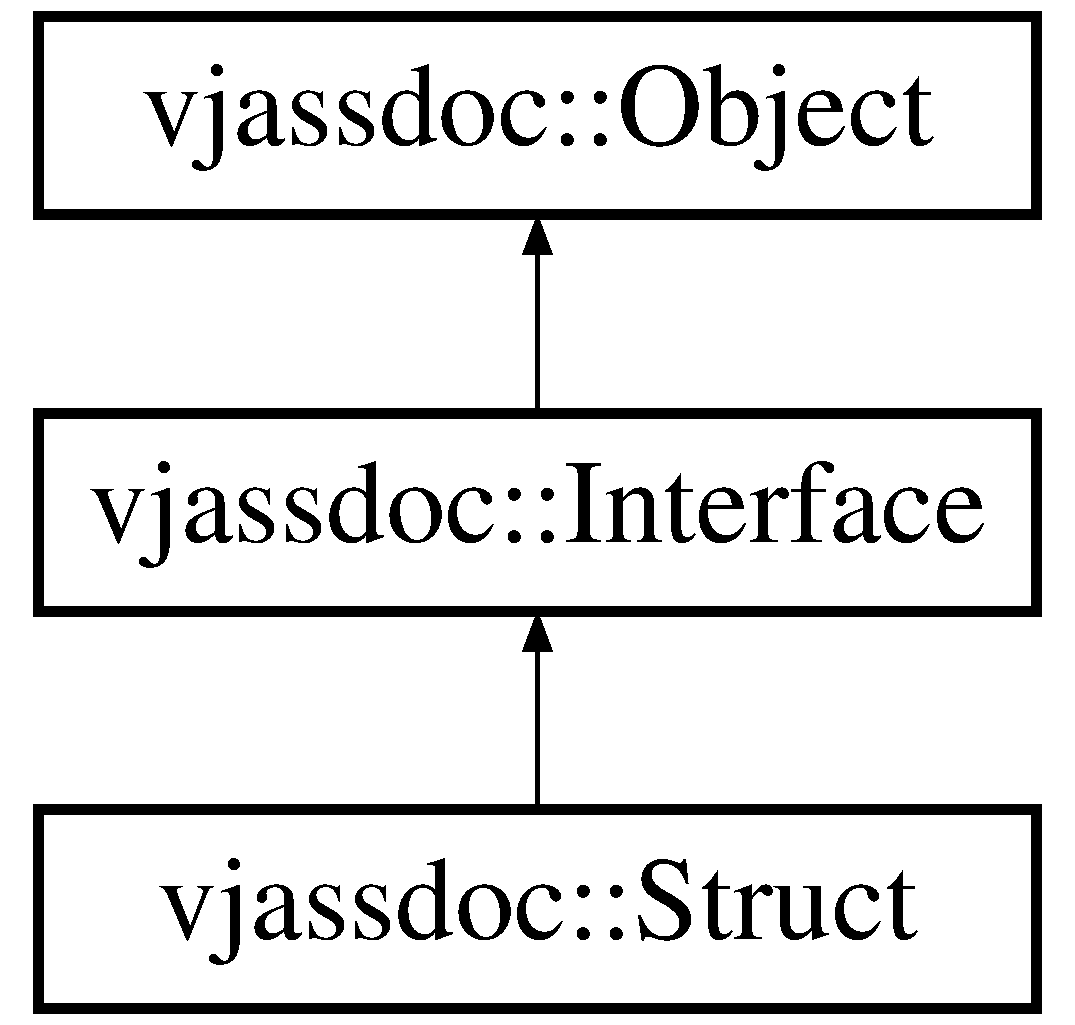
\includegraphics[height=3cm]{classvjassdoc_1_1Interface}
\end{center}
\end{figure}
\subsection*{Public Member Functions}
\begin{CompactItemize}
\item 
\hyperlink{classvjassdoc_1_1Interface_b6c3fb74c0fb4aa7af5cf6dcd7050197}{Interface} (const std::string \&identifier, class \hyperlink{classvjassdoc_1_1SourceFile}{SourceFile} $\ast$sourceFile, unsigned int line, class \hyperlink{classvjassdoc_1_1DocComment}{DocComment} $\ast$docComment, class \hyperlink{classvjassdoc_1_1Library}{Library} $\ast$library, class \hyperlink{classvjassdoc_1_1Scope}{Scope} $\ast$scope, bool isPrivate)
\item 
\hyperlink{classvjassdoc_1_1Interface_6f5c7df2965d2be79bb46d3c4453d862}{Interface} (std::vector$<$ const unsigned char $\ast$ $>$ \&columnVector)
\item 
virtual void \hyperlink{classvjassdoc_1_1Interface_e10d2a4a6acf44897145bf76675b9da1}{init} ()
\item 
virtual void \hyperlink{classvjassdoc_1_1Interface_f0acc07a23eb46eb9f065fb47d55f1a5}{pageNavigation} (std::ofstream \&file) const 
\item 
virtual void \hyperlink{classvjassdoc_1_1Interface_79ed4ee7fd055e3b53fdb9b14749fa0f}{page} (std::ofstream \&file) const 
\item 
virtual std::string \hyperlink{classvjassdoc_1_1Interface_93fbe7323df0502111e576c08376b726}{sqlStatement} () const 
\item 
virtual class \hyperlink{classvjassdoc_1_1Library}{Library} $\ast$ \hyperlink{classvjassdoc_1_1Interface_69ae9cd3e06f91fc2c33ebd6f1b425fe}{library} () const 
\item 
virtual class \hyperlink{classvjassdoc_1_1Scope}{Scope} $\ast$ \hyperlink{classvjassdoc_1_1Interface_407dbdb20eabf2e9f08bf7c459910335}{scope} () const 
\item 
bool \hyperlink{classvjassdoc_1_1Interface_edf12e5dcbcd2ab2afb07164d4ea6e64}{isPrivate} () const 
\item 
void \hyperlink{classvjassdoc_1_1Interface_ed8fce4aaef9f4fa5f3416f3adc02278}{getMemberList} (std::ofstream \&file) const 
\item 
void \hyperlink{classvjassdoc_1_1Interface_055d23bf3a4010668e3a656ea00c9f1e}{getMethodList} (std::ofstream \&file) const 
\end{CompactItemize}


\subsection{Constructor \& Destructor Documentation}
\hypertarget{classvjassdoc_1_1Interface_b6c3fb74c0fb4aa7af5cf6dcd7050197}{
\index{vjassdoc::Interface@{vjassdoc::Interface}!Interface@{Interface}}
\index{Interface@{Interface}!vjassdoc::Interface@{vjassdoc::Interface}}
\subsubsection{\setlength{\rightskip}{0pt plus 5cm}vjassdoc::Interface::Interface (const std::string \& {\em identifier}, class {\bf SourceFile} $\ast$ {\em sourceFile}, unsigned int {\em line}, class {\bf DocComment} $\ast$ {\em docComment}, class {\bf Library} $\ast$ {\em library}, class {\bf Scope} $\ast$ {\em scope}, bool {\em isPrivate})}}
\label{classvjassdoc_1_1Interface_b6c3fb74c0fb4aa7af5cf6dcd7050197}


\hypertarget{classvjassdoc_1_1Interface_6f5c7df2965d2be79bb46d3c4453d862}{
\index{vjassdoc::Interface@{vjassdoc::Interface}!Interface@{Interface}}
\index{Interface@{Interface}!vjassdoc::Interface@{vjassdoc::Interface}}
\subsubsection{\setlength{\rightskip}{0pt plus 5cm}vjassdoc::Interface::Interface (std::vector$<$ const unsigned char $\ast$ $>$ \& {\em columnVector})}}
\label{classvjassdoc_1_1Interface_6f5c7df2965d2be79bb46d3c4453d862}




\subsection{Member Function Documentation}
\hypertarget{classvjassdoc_1_1Interface_e10d2a4a6acf44897145bf76675b9da1}{
\index{vjassdoc::Interface@{vjassdoc::Interface}!init@{init}}
\index{init@{init}!vjassdoc::Interface@{vjassdoc::Interface}}
\subsubsection{\setlength{\rightskip}{0pt plus 5cm}void vjassdoc::Interface::init ()\hspace{0.3cm}{\tt  \mbox{[}virtual\mbox{]}}}}
\label{classvjassdoc_1_1Interface_e10d2a4a6acf44897145bf76675b9da1}




Implements \hyperlink{classvjassdoc_1_1Object_bd43e77dbe80055f5adda67661dfaca4}{vjassdoc::Object}.

Reimplemented in \hyperlink{classvjassdoc_1_1Struct_39dc86da31e526f3a6eb3b6e442156bb}{vjassdoc::Struct}.\hypertarget{classvjassdoc_1_1Interface_f0acc07a23eb46eb9f065fb47d55f1a5}{
\index{vjassdoc::Interface@{vjassdoc::Interface}!pageNavigation@{pageNavigation}}
\index{pageNavigation@{pageNavigation}!vjassdoc::Interface@{vjassdoc::Interface}}
\subsubsection{\setlength{\rightskip}{0pt plus 5cm}void vjassdoc::Interface::pageNavigation (std::ofstream \& {\em file}) const\hspace{0.3cm}{\tt  \mbox{[}virtual\mbox{]}}}}
\label{classvjassdoc_1_1Interface_f0acc07a23eb46eb9f065fb47d55f1a5}




Implements \hyperlink{classvjassdoc_1_1Object_736bbb6719edd8070d8f56c364a2764c}{vjassdoc::Object}.

Reimplemented in \hyperlink{classvjassdoc_1_1Struct_c415c5b26f7385a990339dfbfbbca5dc}{vjassdoc::Struct}.\hypertarget{classvjassdoc_1_1Interface_79ed4ee7fd055e3b53fdb9b14749fa0f}{
\index{vjassdoc::Interface@{vjassdoc::Interface}!page@{page}}
\index{page@{page}!vjassdoc::Interface@{vjassdoc::Interface}}
\subsubsection{\setlength{\rightskip}{0pt plus 5cm}void vjassdoc::Interface::page (std::ofstream \& {\em file}) const\hspace{0.3cm}{\tt  \mbox{[}virtual\mbox{]}}}}
\label{classvjassdoc_1_1Interface_79ed4ee7fd055e3b53fdb9b14749fa0f}




Implements \hyperlink{classvjassdoc_1_1Object_a0489e38956f3507566b1bc6e3e2c8af}{vjassdoc::Object}.

Reimplemented in \hyperlink{classvjassdoc_1_1Struct_bd918c5a1ec7defe1849f4b4e61523f2}{vjassdoc::Struct}.\hypertarget{classvjassdoc_1_1Interface_93fbe7323df0502111e576c08376b726}{
\index{vjassdoc::Interface@{vjassdoc::Interface}!sqlStatement@{sqlStatement}}
\index{sqlStatement@{sqlStatement}!vjassdoc::Interface@{vjassdoc::Interface}}
\subsubsection{\setlength{\rightskip}{0pt plus 5cm}std::string vjassdoc::Interface::sqlStatement () const\hspace{0.3cm}{\tt  \mbox{[}virtual\mbox{]}}}}
\label{classvjassdoc_1_1Interface_93fbe7323df0502111e576c08376b726}




Reimplemented from \hyperlink{classvjassdoc_1_1Object_4e8ebbb0ce5b0bf91ec847b1e4a9f8fc}{vjassdoc::Object}.

Reimplemented in \hyperlink{classvjassdoc_1_1Struct_227d826acdbbe1702941634c90ab7e4e}{vjassdoc::Struct}.\hypertarget{classvjassdoc_1_1Interface_69ae9cd3e06f91fc2c33ebd6f1b425fe}{
\index{vjassdoc::Interface@{vjassdoc::Interface}!library@{library}}
\index{library@{library}!vjassdoc::Interface@{vjassdoc::Interface}}
\subsubsection{\setlength{\rightskip}{0pt plus 5cm}class {\bf Library} $\ast$ vjassdoc::Interface::library () const\hspace{0.3cm}{\tt  \mbox{[}virtual\mbox{]}}}}
\label{classvjassdoc_1_1Interface_69ae9cd3e06f91fc2c33ebd6f1b425fe}




Reimplemented from \hyperlink{classvjassdoc_1_1Object_cc4241505c5bcdd0bbcb08a1b665b3fd}{vjassdoc::Object}.\hypertarget{classvjassdoc_1_1Interface_407dbdb20eabf2e9f08bf7c459910335}{
\index{vjassdoc::Interface@{vjassdoc::Interface}!scope@{scope}}
\index{scope@{scope}!vjassdoc::Interface@{vjassdoc::Interface}}
\subsubsection{\setlength{\rightskip}{0pt plus 5cm}class {\bf Scope} $\ast$ vjassdoc::Interface::scope () const\hspace{0.3cm}{\tt  \mbox{[}virtual\mbox{]}}}}
\label{classvjassdoc_1_1Interface_407dbdb20eabf2e9f08bf7c459910335}




Reimplemented from \hyperlink{classvjassdoc_1_1Object_0738d05b196cc8b9e89d62839d81fc20}{vjassdoc::Object}.\hypertarget{classvjassdoc_1_1Interface_edf12e5dcbcd2ab2afb07164d4ea6e64}{
\index{vjassdoc::Interface@{vjassdoc::Interface}!isPrivate@{isPrivate}}
\index{isPrivate@{isPrivate}!vjassdoc::Interface@{vjassdoc::Interface}}
\subsubsection{\setlength{\rightskip}{0pt plus 5cm}bool vjassdoc::Interface::isPrivate () const\hspace{0.3cm}{\tt  \mbox{[}inline\mbox{]}}}}
\label{classvjassdoc_1_1Interface_edf12e5dcbcd2ab2afb07164d4ea6e64}


\hypertarget{classvjassdoc_1_1Interface_ed8fce4aaef9f4fa5f3416f3adc02278}{
\index{vjassdoc::Interface@{vjassdoc::Interface}!getMemberList@{getMemberList}}
\index{getMemberList@{getMemberList}!vjassdoc::Interface@{vjassdoc::Interface}}
\subsubsection{\setlength{\rightskip}{0pt plus 5cm}void vjassdoc::Interface::getMemberList (std::ofstream \& {\em file}) const}}
\label{classvjassdoc_1_1Interface_ed8fce4aaef9f4fa5f3416f3adc02278}


\hypertarget{classvjassdoc_1_1Interface_055d23bf3a4010668e3a656ea00c9f1e}{
\index{vjassdoc::Interface@{vjassdoc::Interface}!getMethodList@{getMethodList}}
\index{getMethodList@{getMethodList}!vjassdoc::Interface@{vjassdoc::Interface}}
\subsubsection{\setlength{\rightskip}{0pt plus 5cm}void vjassdoc::Interface::getMethodList (std::ofstream \& {\em file}) const}}
\label{classvjassdoc_1_1Interface_055d23bf3a4010668e3a656ea00c9f1e}




The documentation for this class was generated from the following files:\begin{CompactItemize}
\item 
src/\hyperlink{interface_8h}{interface.h}\item 
src/\hyperlink{interface_8cpp}{interface.cpp}\end{CompactItemize}

\hypertarget{classvjassdoc_1_1Keyword}{
\section{vjassdoc::Keyword Class Reference}
\label{classvjassdoc_1_1Keyword}\index{vjassdoc::Keyword@{vjassdoc::Keyword}}
}
{\tt \#include $<$keyword.h$>$}

Inheritance diagram for vjassdoc::Keyword::\begin{figure}[H]
\begin{center}
\leavevmode
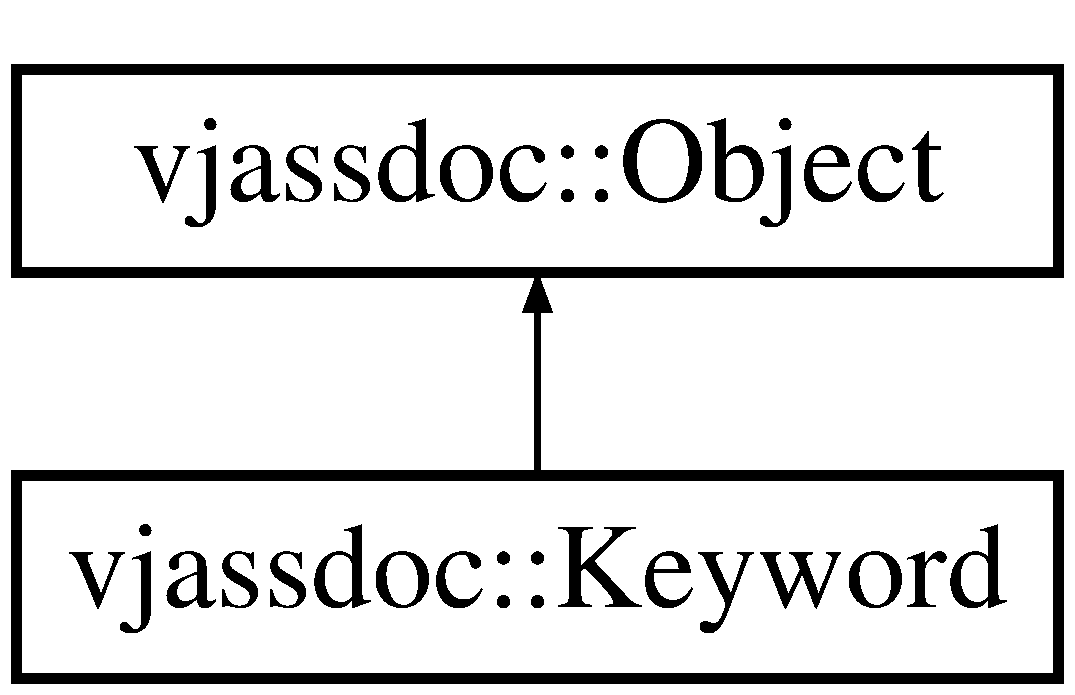
\includegraphics[height=2cm]{classvjassdoc_1_1Keyword}
\end{center}
\end{figure}
\subsection*{Public Member Functions}
\begin{CompactItemize}
\item 
\hyperlink{classvjassdoc_1_1Keyword_f9216d9602f71a8b10d25d6c61412fc2}{Keyword} (const std::string \&identifier, class \hyperlink{classvjassdoc_1_1SourceFile}{SourceFile} $\ast$sourceFile, unsigned int line, class \hyperlink{classvjassdoc_1_1DocComment}{DocComment} $\ast$docComment, class \hyperlink{classvjassdoc_1_1Library}{Library} $\ast$library, class \hyperlink{classvjassdoc_1_1Scope}{Scope} $\ast$scope, bool isPrivate)
\item 
\hyperlink{classvjassdoc_1_1Keyword_b12dde7146b5bb943108d520599d988d}{Keyword} (std::vector$<$ const unsigned char $\ast$ $>$ \&columnVector)
\item 
virtual void \hyperlink{classvjassdoc_1_1Keyword_0aeec733c7c55ff51c8b1ba58af18ed9}{init} ()
\item 
virtual void \hyperlink{classvjassdoc_1_1Keyword_c8950d4ece99a58cc664daf5f652f37c}{pageNavigation} (std::ofstream \&file) const 
\item 
virtual void \hyperlink{classvjassdoc_1_1Keyword_207c989cefeeb0857adb76aa5d7bd842}{page} (std::ofstream \&file) const 
\item 
virtual std::string \hyperlink{classvjassdoc_1_1Keyword_b2d197337624e89955564ac684bfd5ad}{sqlStatement} () const 
\item 
virtual class \hyperlink{classvjassdoc_1_1Library}{Library} $\ast$ \hyperlink{classvjassdoc_1_1Keyword_9496b5c2a1eedee46d27dd166608b12f}{library} () const 
\item 
virtual class \hyperlink{classvjassdoc_1_1Scope}{Scope} $\ast$ \hyperlink{classvjassdoc_1_1Keyword_5524a7a3029192c2c460a1914cce63e3}{scope} () const 
\item 
bool \hyperlink{classvjassdoc_1_1Keyword_f07683a667bfdfaa4dfa82da6844af97}{isPrivate} () const 
\end{CompactItemize}


\subsection{Constructor \& Destructor Documentation}
\hypertarget{classvjassdoc_1_1Keyword_f9216d9602f71a8b10d25d6c61412fc2}{
\index{vjassdoc::Keyword@{vjassdoc::Keyword}!Keyword@{Keyword}}
\index{Keyword@{Keyword}!vjassdoc::Keyword@{vjassdoc::Keyword}}
\subsubsection{\setlength{\rightskip}{0pt plus 5cm}vjassdoc::Keyword::Keyword (const std::string \& {\em identifier}, class {\bf SourceFile} $\ast$ {\em sourceFile}, unsigned int {\em line}, class {\bf DocComment} $\ast$ {\em docComment}, class {\bf Library} $\ast$ {\em library}, class {\bf Scope} $\ast$ {\em scope}, bool {\em isPrivate})}}
\label{classvjassdoc_1_1Keyword_f9216d9602f71a8b10d25d6c61412fc2}


\hypertarget{classvjassdoc_1_1Keyword_b12dde7146b5bb943108d520599d988d}{
\index{vjassdoc::Keyword@{vjassdoc::Keyword}!Keyword@{Keyword}}
\index{Keyword@{Keyword}!vjassdoc::Keyword@{vjassdoc::Keyword}}
\subsubsection{\setlength{\rightskip}{0pt plus 5cm}vjassdoc::Keyword::Keyword (std::vector$<$ const unsigned char $\ast$ $>$ \& {\em columnVector})}}
\label{classvjassdoc_1_1Keyword_b12dde7146b5bb943108d520599d988d}




\subsection{Member Function Documentation}
\hypertarget{classvjassdoc_1_1Keyword_0aeec733c7c55ff51c8b1ba58af18ed9}{
\index{vjassdoc::Keyword@{vjassdoc::Keyword}!init@{init}}
\index{init@{init}!vjassdoc::Keyword@{vjassdoc::Keyword}}
\subsubsection{\setlength{\rightskip}{0pt plus 5cm}void vjassdoc::Keyword::init ()\hspace{0.3cm}{\tt  \mbox{[}virtual\mbox{]}}}}
\label{classvjassdoc_1_1Keyword_0aeec733c7c55ff51c8b1ba58af18ed9}




Implements \hyperlink{classvjassdoc_1_1Object_bd43e77dbe80055f5adda67661dfaca4}{vjassdoc::Object}.\hypertarget{classvjassdoc_1_1Keyword_c8950d4ece99a58cc664daf5f652f37c}{
\index{vjassdoc::Keyword@{vjassdoc::Keyword}!pageNavigation@{pageNavigation}}
\index{pageNavigation@{pageNavigation}!vjassdoc::Keyword@{vjassdoc::Keyword}}
\subsubsection{\setlength{\rightskip}{0pt plus 5cm}void vjassdoc::Keyword::pageNavigation (std::ofstream \& {\em file}) const\hspace{0.3cm}{\tt  \mbox{[}virtual\mbox{]}}}}
\label{classvjassdoc_1_1Keyword_c8950d4ece99a58cc664daf5f652f37c}




Implements \hyperlink{classvjassdoc_1_1Object_736bbb6719edd8070d8f56c364a2764c}{vjassdoc::Object}.\hypertarget{classvjassdoc_1_1Keyword_207c989cefeeb0857adb76aa5d7bd842}{
\index{vjassdoc::Keyword@{vjassdoc::Keyword}!page@{page}}
\index{page@{page}!vjassdoc::Keyword@{vjassdoc::Keyword}}
\subsubsection{\setlength{\rightskip}{0pt plus 5cm}void vjassdoc::Keyword::page (std::ofstream \& {\em file}) const\hspace{0.3cm}{\tt  \mbox{[}virtual\mbox{]}}}}
\label{classvjassdoc_1_1Keyword_207c989cefeeb0857adb76aa5d7bd842}




Implements \hyperlink{classvjassdoc_1_1Object_a0489e38956f3507566b1bc6e3e2c8af}{vjassdoc::Object}.\hypertarget{classvjassdoc_1_1Keyword_b2d197337624e89955564ac684bfd5ad}{
\index{vjassdoc::Keyword@{vjassdoc::Keyword}!sqlStatement@{sqlStatement}}
\index{sqlStatement@{sqlStatement}!vjassdoc::Keyword@{vjassdoc::Keyword}}
\subsubsection{\setlength{\rightskip}{0pt plus 5cm}std::string vjassdoc::Keyword::sqlStatement () const\hspace{0.3cm}{\tt  \mbox{[}virtual\mbox{]}}}}
\label{classvjassdoc_1_1Keyword_b2d197337624e89955564ac684bfd5ad}




Reimplemented from \hyperlink{classvjassdoc_1_1Object_4e8ebbb0ce5b0bf91ec847b1e4a9f8fc}{vjassdoc::Object}.\hypertarget{classvjassdoc_1_1Keyword_9496b5c2a1eedee46d27dd166608b12f}{
\index{vjassdoc::Keyword@{vjassdoc::Keyword}!library@{library}}
\index{library@{library}!vjassdoc::Keyword@{vjassdoc::Keyword}}
\subsubsection{\setlength{\rightskip}{0pt plus 5cm}class {\bf Library} $\ast$ vjassdoc::Keyword::library () const\hspace{0.3cm}{\tt  \mbox{[}virtual\mbox{]}}}}
\label{classvjassdoc_1_1Keyword_9496b5c2a1eedee46d27dd166608b12f}




Reimplemented from \hyperlink{classvjassdoc_1_1Object_cc4241505c5bcdd0bbcb08a1b665b3fd}{vjassdoc::Object}.\hypertarget{classvjassdoc_1_1Keyword_5524a7a3029192c2c460a1914cce63e3}{
\index{vjassdoc::Keyword@{vjassdoc::Keyword}!scope@{scope}}
\index{scope@{scope}!vjassdoc::Keyword@{vjassdoc::Keyword}}
\subsubsection{\setlength{\rightskip}{0pt plus 5cm}class {\bf Scope} $\ast$ vjassdoc::Keyword::scope () const\hspace{0.3cm}{\tt  \mbox{[}virtual\mbox{]}}}}
\label{classvjassdoc_1_1Keyword_5524a7a3029192c2c460a1914cce63e3}




Reimplemented from \hyperlink{classvjassdoc_1_1Object_0738d05b196cc8b9e89d62839d81fc20}{vjassdoc::Object}.\hypertarget{classvjassdoc_1_1Keyword_f07683a667bfdfaa4dfa82da6844af97}{
\index{vjassdoc::Keyword@{vjassdoc::Keyword}!isPrivate@{isPrivate}}
\index{isPrivate@{isPrivate}!vjassdoc::Keyword@{vjassdoc::Keyword}}
\subsubsection{\setlength{\rightskip}{0pt plus 5cm}bool vjassdoc::Keyword::isPrivate () const\hspace{0.3cm}{\tt  \mbox{[}inline\mbox{]}}}}
\label{classvjassdoc_1_1Keyword_f07683a667bfdfaa4dfa82da6844af97}




The documentation for this class was generated from the following files:\begin{CompactItemize}
\item 
src/\hyperlink{keyword_8h}{keyword.h}\item 
src/\hyperlink{keyword_8cpp}{keyword.cpp}\end{CompactItemize}

\hypertarget{classvjassdoc_1_1Library}{
\section{vjassdoc::Library Class Reference}
\label{classvjassdoc_1_1Library}\index{vjassdoc::Library@{vjassdoc::Library}}
}
{\tt \#include $<$library.h$>$}

Inheritance diagram for vjassdoc::Library::\begin{figure}[H]
\begin{center}
\leavevmode
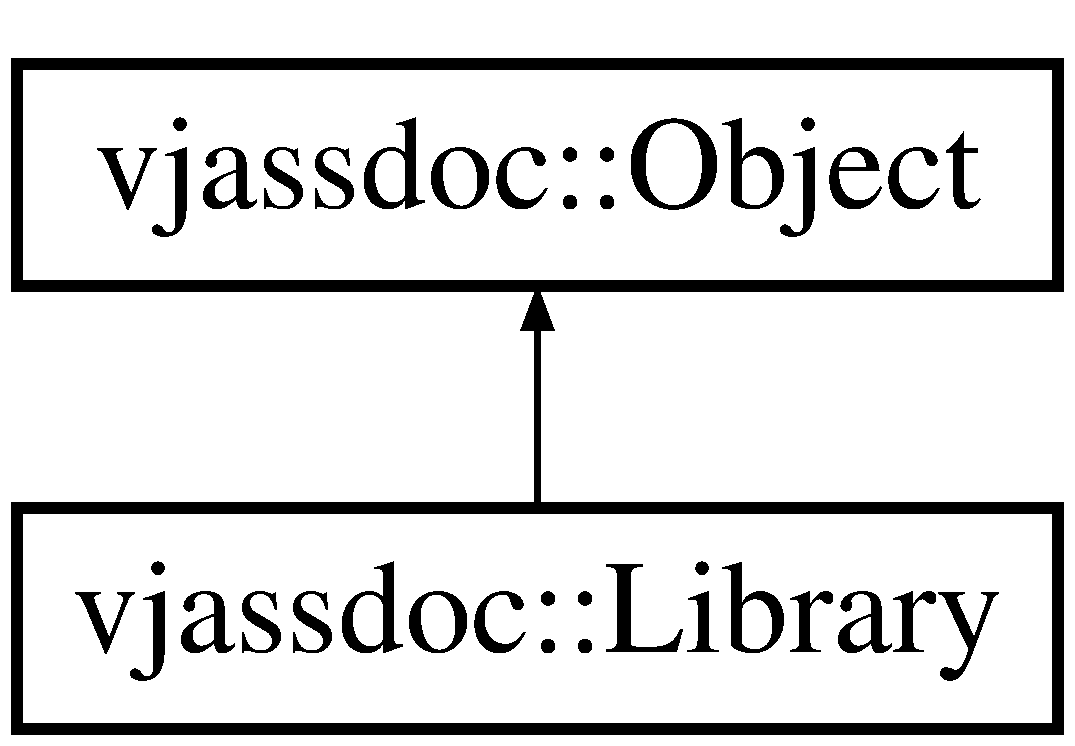
\includegraphics[height=2cm]{classvjassdoc_1_1Library}
\end{center}
\end{figure}
\subsection*{Public Member Functions}
\begin{CompactItemize}
\item 
\hyperlink{classvjassdoc_1_1Library_9f69ca5b7692f0351f1ac263c9b3bf28}{Library} (const std::string \&identifier, class \hyperlink{classvjassdoc_1_1SourceFile}{SourceFile} $\ast$sourceFile, unsigned int line, class \hyperlink{classvjassdoc_1_1DocComment}{DocComment} $\ast$docComment, bool isOnce, const std::string \&initializerExpression, std::list$<$ std::string $>$ $\ast$requirementExpressions)
\item 
\hyperlink{classvjassdoc_1_1Library_2e9ab1441cf3e30919312c8f3644f190}{Library} (std::vector$<$ const unsigned char $\ast$ $>$ \&columnVector)
\item 
virtual \hyperlink{classvjassdoc_1_1Library_412120c44682db1ae36a04254583eb75}{$\sim$Library} ()
\item 
virtual void \hyperlink{classvjassdoc_1_1Library_d1bbc6153d45c040be60419a6708bd7d}{init} ()
\item 
virtual void \hyperlink{classvjassdoc_1_1Library_782d6d0f5d58756924f0ab413821967a}{pageNavigation} (std::ofstream \&file) const 
\item 
virtual void \hyperlink{classvjassdoc_1_1Library_b49718631812ed3a5bcfe0a5bdf7595e}{page} (std::ofstream \&file) const 
\item 
virtual std::string \hyperlink{classvjassdoc_1_1Library_21dd8d48803fa96b2b22cb9846c9b915}{sqlStatement} () const 
\item 
bool \hyperlink{classvjassdoc_1_1Library_c80f46bebe911d249c7d7fdbc9fa3f5b}{isOnce} () const 
\item 
class \hyperlink{classvjassdoc_1_1Function}{Function} $\ast$ \hyperlink{classvjassdoc_1_1Library_99bc875c90c8ca4062dcddc8c4f7c8c6}{initializer} () const 
\item 
std::list$<$ class \hyperlink{classvjassdoc_1_1Library}{Library} $\ast$ $>$ $\ast$ \hyperlink{classvjassdoc_1_1Library_aa5627b4a2e5b730d3dbc7d141a0e6ef}{requirement} () const 
\end{CompactItemize}


\subsection{Constructor \& Destructor Documentation}
\hypertarget{classvjassdoc_1_1Library_9f69ca5b7692f0351f1ac263c9b3bf28}{
\index{vjassdoc::Library@{vjassdoc::Library}!Library@{Library}}
\index{Library@{Library}!vjassdoc::Library@{vjassdoc::Library}}
\subsubsection{\setlength{\rightskip}{0pt plus 5cm}vjassdoc::Library::Library (const std::string \& {\em identifier}, class {\bf SourceFile} $\ast$ {\em sourceFile}, unsigned int {\em line}, class {\bf DocComment} $\ast$ {\em docComment}, bool {\em isOnce}, const std::string \& {\em initializerExpression}, std::list$<$ std::string $>$ $\ast$ {\em requirementExpressions})}}
\label{classvjassdoc_1_1Library_9f69ca5b7692f0351f1ac263c9b3bf28}


\hypertarget{classvjassdoc_1_1Library_2e9ab1441cf3e30919312c8f3644f190}{
\index{vjassdoc::Library@{vjassdoc::Library}!Library@{Library}}
\index{Library@{Library}!vjassdoc::Library@{vjassdoc::Library}}
\subsubsection{\setlength{\rightskip}{0pt plus 5cm}vjassdoc::Library::Library (std::vector$<$ const unsigned char $\ast$ $>$ \& {\em columnVector})}}
\label{classvjassdoc_1_1Library_2e9ab1441cf3e30919312c8f3644f190}


\hypertarget{classvjassdoc_1_1Library_412120c44682db1ae36a04254583eb75}{
\index{vjassdoc::Library@{vjassdoc::Library}!$\sim$Library@{$\sim$Library}}
\index{$\sim$Library@{$\sim$Library}!vjassdoc::Library@{vjassdoc::Library}}
\subsubsection{\setlength{\rightskip}{0pt plus 5cm}vjassdoc::Library::$\sim$Library ()\hspace{0.3cm}{\tt  \mbox{[}virtual\mbox{]}}}}
\label{classvjassdoc_1_1Library_412120c44682db1ae36a04254583eb75}




\subsection{Member Function Documentation}
\hypertarget{classvjassdoc_1_1Library_d1bbc6153d45c040be60419a6708bd7d}{
\index{vjassdoc::Library@{vjassdoc::Library}!init@{init}}
\index{init@{init}!vjassdoc::Library@{vjassdoc::Library}}
\subsubsection{\setlength{\rightskip}{0pt plus 5cm}void vjassdoc::Library::init ()\hspace{0.3cm}{\tt  \mbox{[}virtual\mbox{]}}}}
\label{classvjassdoc_1_1Library_d1bbc6153d45c040be60419a6708bd7d}




Implements \hyperlink{classvjassdoc_1_1Object_bd43e77dbe80055f5adda67661dfaca4}{vjassdoc::Object}.\hypertarget{classvjassdoc_1_1Library_782d6d0f5d58756924f0ab413821967a}{
\index{vjassdoc::Library@{vjassdoc::Library}!pageNavigation@{pageNavigation}}
\index{pageNavigation@{pageNavigation}!vjassdoc::Library@{vjassdoc::Library}}
\subsubsection{\setlength{\rightskip}{0pt plus 5cm}void vjassdoc::Library::pageNavigation (std::ofstream \& {\em file}) const\hspace{0.3cm}{\tt  \mbox{[}virtual\mbox{]}}}}
\label{classvjassdoc_1_1Library_782d6d0f5d58756924f0ab413821967a}




Implements \hyperlink{classvjassdoc_1_1Object_736bbb6719edd8070d8f56c364a2764c}{vjassdoc::Object}.\hypertarget{classvjassdoc_1_1Library_b49718631812ed3a5bcfe0a5bdf7595e}{
\index{vjassdoc::Library@{vjassdoc::Library}!page@{page}}
\index{page@{page}!vjassdoc::Library@{vjassdoc::Library}}
\subsubsection{\setlength{\rightskip}{0pt plus 5cm}void vjassdoc::Library::page (std::ofstream \& {\em file}) const\hspace{0.3cm}{\tt  \mbox{[}virtual\mbox{]}}}}
\label{classvjassdoc_1_1Library_b49718631812ed3a5bcfe0a5bdf7595e}




Implements \hyperlink{classvjassdoc_1_1Object_a0489e38956f3507566b1bc6e3e2c8af}{vjassdoc::Object}.\hypertarget{classvjassdoc_1_1Library_21dd8d48803fa96b2b22cb9846c9b915}{
\index{vjassdoc::Library@{vjassdoc::Library}!sqlStatement@{sqlStatement}}
\index{sqlStatement@{sqlStatement}!vjassdoc::Library@{vjassdoc::Library}}
\subsubsection{\setlength{\rightskip}{0pt plus 5cm}std::string vjassdoc::Library::sqlStatement () const\hspace{0.3cm}{\tt  \mbox{[}virtual\mbox{]}}}}
\label{classvjassdoc_1_1Library_21dd8d48803fa96b2b22cb9846c9b915}




Reimplemented from \hyperlink{classvjassdoc_1_1Object_4e8ebbb0ce5b0bf91ec847b1e4a9f8fc}{vjassdoc::Object}.\hypertarget{classvjassdoc_1_1Library_c80f46bebe911d249c7d7fdbc9fa3f5b}{
\index{vjassdoc::Library@{vjassdoc::Library}!isOnce@{isOnce}}
\index{isOnce@{isOnce}!vjassdoc::Library@{vjassdoc::Library}}
\subsubsection{\setlength{\rightskip}{0pt plus 5cm}bool vjassdoc::Library::isOnce () const\hspace{0.3cm}{\tt  \mbox{[}inline\mbox{]}}}}
\label{classvjassdoc_1_1Library_c80f46bebe911d249c7d7fdbc9fa3f5b}


\hypertarget{classvjassdoc_1_1Library_99bc875c90c8ca4062dcddc8c4f7c8c6}{
\index{vjassdoc::Library@{vjassdoc::Library}!initializer@{initializer}}
\index{initializer@{initializer}!vjassdoc::Library@{vjassdoc::Library}}
\subsubsection{\setlength{\rightskip}{0pt plus 5cm}class {\bf Function} $\ast$ vjassdoc::Library::initializer () const\hspace{0.3cm}{\tt  \mbox{[}inline\mbox{]}}}}
\label{classvjassdoc_1_1Library_99bc875c90c8ca4062dcddc8c4f7c8c6}


\hypertarget{classvjassdoc_1_1Library_aa5627b4a2e5b730d3dbc7d141a0e6ef}{
\index{vjassdoc::Library@{vjassdoc::Library}!requirement@{requirement}}
\index{requirement@{requirement}!vjassdoc::Library@{vjassdoc::Library}}
\subsubsection{\setlength{\rightskip}{0pt plus 5cm}std::list$<$ class {\bf Library} $\ast$ $>$ $\ast$ vjassdoc::Library::requirement () const\hspace{0.3cm}{\tt  \mbox{[}inline\mbox{]}}}}
\label{classvjassdoc_1_1Library_aa5627b4a2e5b730d3dbc7d141a0e6ef}




The documentation for this class was generated from the following files:\begin{CompactItemize}
\item 
src/\hyperlink{library_8h}{library.h}\item 
src/\hyperlink{library_8cpp}{library.cpp}\end{CompactItemize}

\hypertarget{classvjassdoc_1_1Member}{
\section{vjassdoc::Member Class Reference}
\label{classvjassdoc_1_1Member}\index{vjassdoc::Member@{vjassdoc::Member}}
}
{\tt \#include $<$member.h$>$}

Inheritance diagram for vjassdoc::Member::\begin{figure}[H]
\begin{center}
\leavevmode
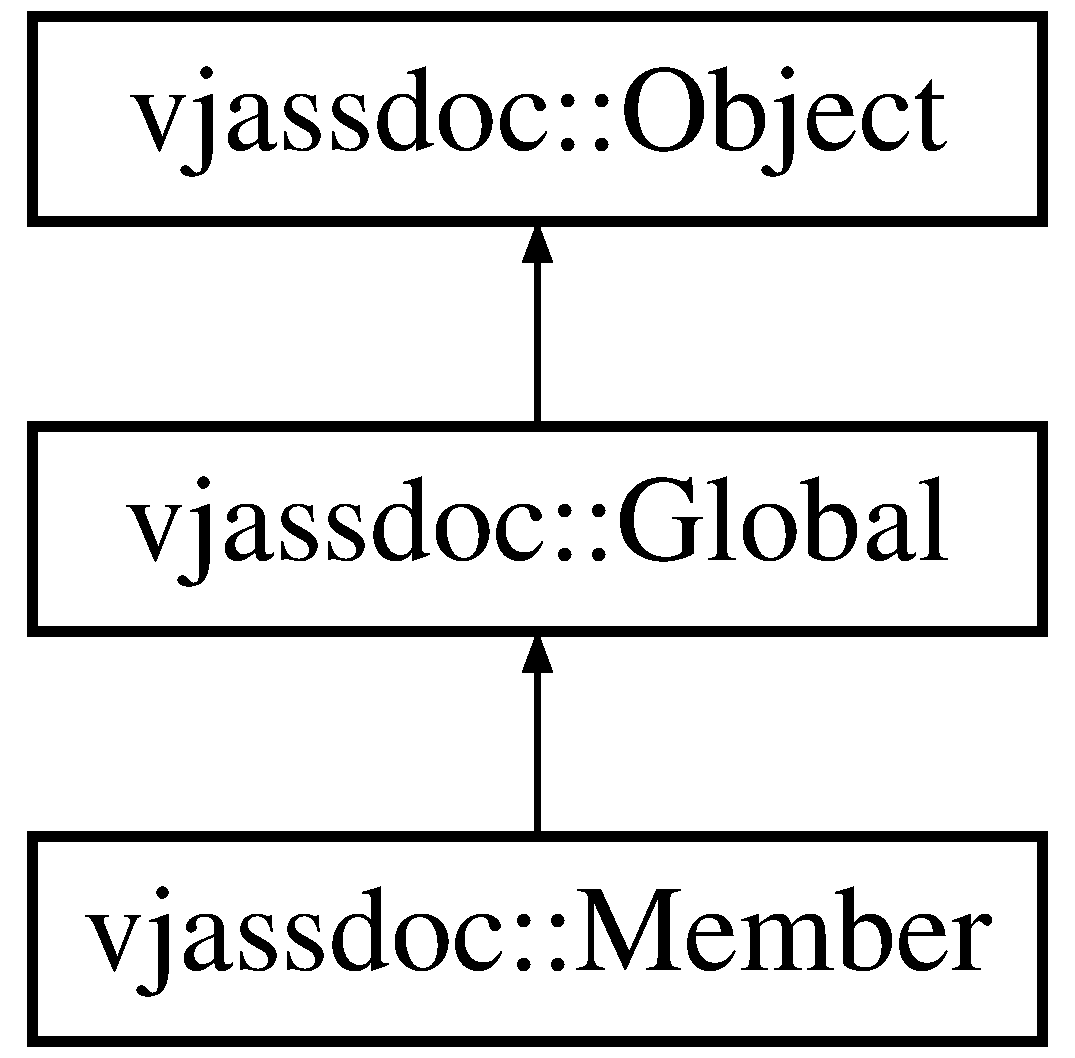
\includegraphics[height=3cm]{classvjassdoc_1_1Member}
\end{center}
\end{figure}
\subsection*{Public Member Functions}
\begin{CompactItemize}
\item 
\hyperlink{classvjassdoc_1_1Member_7d85b6523c38a202e0c5e05c2b28c51a}{Member} (const std::string \&identifier, class \hyperlink{classvjassdoc_1_1SourceFile}{SourceFile} $\ast$sourceFile, unsigned int line, class \hyperlink{classvjassdoc_1_1DocComment}{DocComment} $\ast$docComment, class \hyperlink{classvjassdoc_1_1Library}{Library} $\ast$library, class \hyperlink{classvjassdoc_1_1Scope}{Scope} $\ast$scope, bool isPrivate, bool isPublic, bool isConstant, const std::string \&typeExpression, const std::string \&valueExpression, const std::string \&sizeExpression, class \hyperlink{classvjassdoc_1_1Object}{Object} $\ast$container, bool isStatic, bool isDelegate)
\item 
\hyperlink{classvjassdoc_1_1Member_6a4d211407bef23d4a7cd4c70f5ca8f7}{Member} (std::vector$<$ const unsigned char $\ast$ $>$ \&columnVector)
\item 
virtual void \hyperlink{classvjassdoc_1_1Member_eccac74ca5ea37e82d322c20b5aa2efc}{init} ()
\item 
virtual void \hyperlink{classvjassdoc_1_1Member_fa8e020175714b1f03a3696cc935941f}{pageNavigation} (std::ofstream \&file) const 
\item 
virtual void \hyperlink{classvjassdoc_1_1Member_2bd66eba1882dfb2dcbf2552b42d1346}{page} (std::ofstream \&file) const 
\item 
virtual std::string \hyperlink{classvjassdoc_1_1Member_ad210521f998bd4c8be5f8af3ae74cf1}{sqlStatement} () const 
\item 
virtual class \hyperlink{classvjassdoc_1_1Object}{Object} $\ast$ \hyperlink{classvjassdoc_1_1Member_313ed6d74338700b34409ccad8dc5360}{container} () const 
\item 
bool \hyperlink{classvjassdoc_1_1Member_f832d9e8d585167eb8cb3e9051b03ba0}{isStatic} () const 
\item 
bool \hyperlink{classvjassdoc_1_1Member_d6df00fb8a3bfe32915e00c7ddb8fbbe}{isDelegate} () const 
\end{CompactItemize}


\subsection{Constructor \& Destructor Documentation}
\hypertarget{classvjassdoc_1_1Member_7d85b6523c38a202e0c5e05c2b28c51a}{
\index{vjassdoc::Member@{vjassdoc::Member}!Member@{Member}}
\index{Member@{Member}!vjassdoc::Member@{vjassdoc::Member}}
\subsubsection{\setlength{\rightskip}{0pt plus 5cm}vjassdoc::Member::Member (const std::string \& {\em identifier}, class {\bf SourceFile} $\ast$ {\em sourceFile}, unsigned int {\em line}, class {\bf DocComment} $\ast$ {\em docComment}, class {\bf Library} $\ast$ {\em library}, class {\bf Scope} $\ast$ {\em scope}, bool {\em isPrivate}, bool {\em isPublic}, bool {\em isConstant}, const std::string \& {\em typeExpression}, const std::string \& {\em valueExpression}, const std::string \& {\em sizeExpression}, class {\bf Object} $\ast$ {\em container}, bool {\em isStatic}, bool {\em isDelegate})}}
\label{classvjassdoc_1_1Member_7d85b6523c38a202e0c5e05c2b28c51a}


\hypertarget{classvjassdoc_1_1Member_6a4d211407bef23d4a7cd4c70f5ca8f7}{
\index{vjassdoc::Member@{vjassdoc::Member}!Member@{Member}}
\index{Member@{Member}!vjassdoc::Member@{vjassdoc::Member}}
\subsubsection{\setlength{\rightskip}{0pt plus 5cm}vjassdoc::Member::Member (std::vector$<$ const unsigned char $\ast$ $>$ \& {\em columnVector})}}
\label{classvjassdoc_1_1Member_6a4d211407bef23d4a7cd4c70f5ca8f7}




\subsection{Member Function Documentation}
\hypertarget{classvjassdoc_1_1Member_eccac74ca5ea37e82d322c20b5aa2efc}{
\index{vjassdoc::Member@{vjassdoc::Member}!init@{init}}
\index{init@{init}!vjassdoc::Member@{vjassdoc::Member}}
\subsubsection{\setlength{\rightskip}{0pt plus 5cm}void vjassdoc::Member::init ()\hspace{0.3cm}{\tt  \mbox{[}virtual\mbox{]}}}}
\label{classvjassdoc_1_1Member_eccac74ca5ea37e82d322c20b5aa2efc}




Reimplemented from \hyperlink{classvjassdoc_1_1Global_9e6189cfd577f0453988e8c8c6eec04d}{vjassdoc::Global}.\hypertarget{classvjassdoc_1_1Member_fa8e020175714b1f03a3696cc935941f}{
\index{vjassdoc::Member@{vjassdoc::Member}!pageNavigation@{pageNavigation}}
\index{pageNavigation@{pageNavigation}!vjassdoc::Member@{vjassdoc::Member}}
\subsubsection{\setlength{\rightskip}{0pt plus 5cm}void vjassdoc::Member::pageNavigation (std::ofstream \& {\em file}) const\hspace{0.3cm}{\tt  \mbox{[}virtual\mbox{]}}}}
\label{classvjassdoc_1_1Member_fa8e020175714b1f03a3696cc935941f}




Reimplemented from \hyperlink{classvjassdoc_1_1Global_8c5209b5652d3633feb1d7fab796b439}{vjassdoc::Global}.\hypertarget{classvjassdoc_1_1Member_2bd66eba1882dfb2dcbf2552b42d1346}{
\index{vjassdoc::Member@{vjassdoc::Member}!page@{page}}
\index{page@{page}!vjassdoc::Member@{vjassdoc::Member}}
\subsubsection{\setlength{\rightskip}{0pt plus 5cm}void vjassdoc::Member::page (std::ofstream \& {\em file}) const\hspace{0.3cm}{\tt  \mbox{[}virtual\mbox{]}}}}
\label{classvjassdoc_1_1Member_2bd66eba1882dfb2dcbf2552b42d1346}




Reimplemented from \hyperlink{classvjassdoc_1_1Global_1b8fefe2b9c895c122a822bac0383f1b}{vjassdoc::Global}.\hypertarget{classvjassdoc_1_1Member_ad210521f998bd4c8be5f8af3ae74cf1}{
\index{vjassdoc::Member@{vjassdoc::Member}!sqlStatement@{sqlStatement}}
\index{sqlStatement@{sqlStatement}!vjassdoc::Member@{vjassdoc::Member}}
\subsubsection{\setlength{\rightskip}{0pt plus 5cm}std::string vjassdoc::Member::sqlStatement () const\hspace{0.3cm}{\tt  \mbox{[}virtual\mbox{]}}}}
\label{classvjassdoc_1_1Member_ad210521f998bd4c8be5f8af3ae74cf1}




Reimplemented from \hyperlink{classvjassdoc_1_1Global_4e9a8ea0c8bc34f6980d31676e497531}{vjassdoc::Global}.\hypertarget{classvjassdoc_1_1Member_313ed6d74338700b34409ccad8dc5360}{
\index{vjassdoc::Member@{vjassdoc::Member}!container@{container}}
\index{container@{container}!vjassdoc::Member@{vjassdoc::Member}}
\subsubsection{\setlength{\rightskip}{0pt plus 5cm}class {\bf Object} $\ast$ vjassdoc::Member::container () const\hspace{0.3cm}{\tt  \mbox{[}virtual\mbox{]}}}}
\label{classvjassdoc_1_1Member_313ed6d74338700b34409ccad8dc5360}




Reimplemented from \hyperlink{classvjassdoc_1_1Object_b3729c3b063682f94b43a42546c90e96}{vjassdoc::Object}.\hypertarget{classvjassdoc_1_1Member_f832d9e8d585167eb8cb3e9051b03ba0}{
\index{vjassdoc::Member@{vjassdoc::Member}!isStatic@{isStatic}}
\index{isStatic@{isStatic}!vjassdoc::Member@{vjassdoc::Member}}
\subsubsection{\setlength{\rightskip}{0pt plus 5cm}bool vjassdoc::Member::isStatic () const\hspace{0.3cm}{\tt  \mbox{[}inline\mbox{]}}}}
\label{classvjassdoc_1_1Member_f832d9e8d585167eb8cb3e9051b03ba0}


\hypertarget{classvjassdoc_1_1Member_d6df00fb8a3bfe32915e00c7ddb8fbbe}{
\index{vjassdoc::Member@{vjassdoc::Member}!isDelegate@{isDelegate}}
\index{isDelegate@{isDelegate}!vjassdoc::Member@{vjassdoc::Member}}
\subsubsection{\setlength{\rightskip}{0pt plus 5cm}bool vjassdoc::Member::isDelegate () const\hspace{0.3cm}{\tt  \mbox{[}inline\mbox{]}}}}
\label{classvjassdoc_1_1Member_d6df00fb8a3bfe32915e00c7ddb8fbbe}




The documentation for this class was generated from the following files:\begin{CompactItemize}
\item 
src/\hyperlink{member_8h}{member.h}\item 
src/\hyperlink{member_8cpp}{member.cpp}\end{CompactItemize}

\hypertarget{classvjassdoc_1_1Method}{
\section{vjassdoc::Method Class Reference}
\label{classvjassdoc_1_1Method}\index{vjassdoc::Method@{vjassdoc::Method}}
}
{\tt \#include $<$method.h$>$}

Inheritance diagram for vjassdoc::Method::\begin{figure}[H]
\begin{center}
\leavevmode
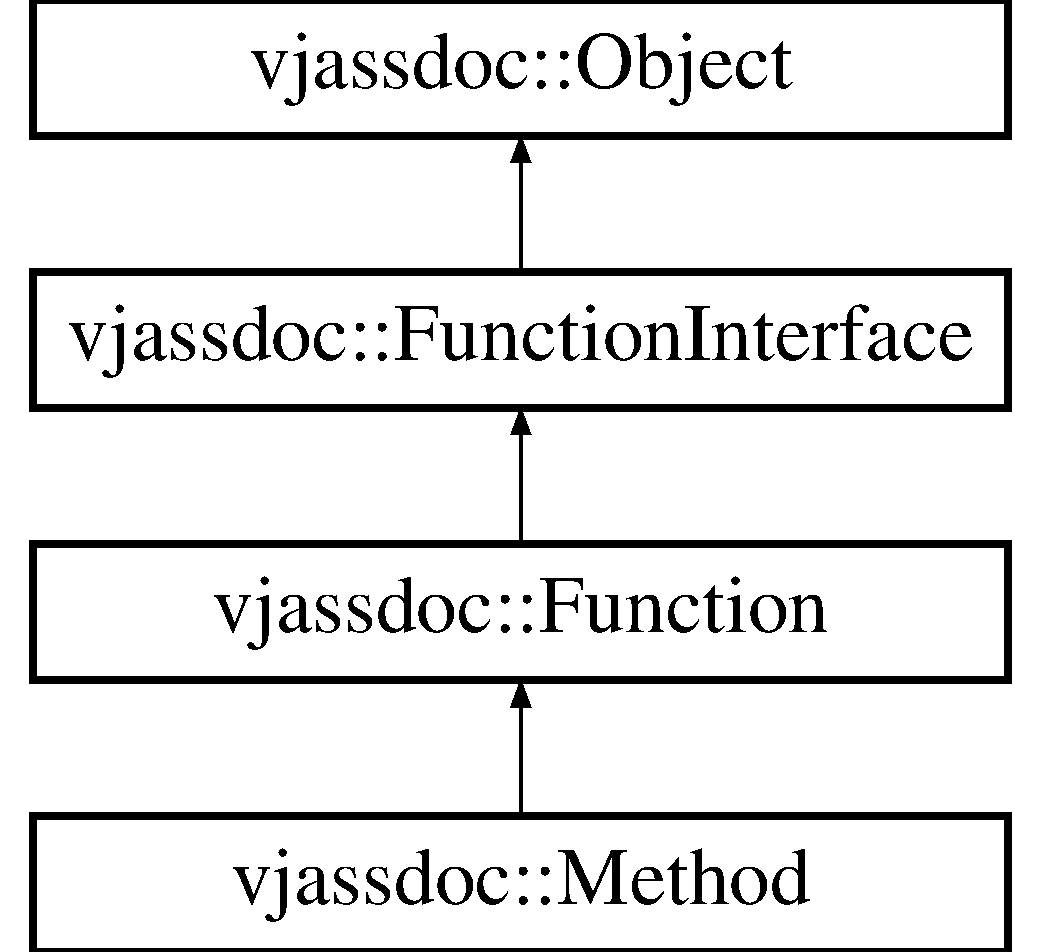
\includegraphics[height=4cm]{classvjassdoc_1_1Method}
\end{center}
\end{figure}
\subsection*{Public Member Functions}
\begin{CompactItemize}
\item 
\hyperlink{classvjassdoc_1_1Method_b8d4ae00da196848f84771240386414a}{Method} (const std::string \&identifier, class \hyperlink{classvjassdoc_1_1SourceFile}{SourceFile} $\ast$sourceFile, unsigned int line, class \hyperlink{classvjassdoc_1_1DocComment}{DocComment} $\ast$docComment, class \hyperlink{classvjassdoc_1_1Library}{Library} $\ast$library, class \hyperlink{classvjassdoc_1_1Scope}{Scope} $\ast$scope, bool isPrivate, std::list$<$ std::string $>$ $\ast$parameterTypeExpressions, std::list$<$ std::string $>$ $\ast$parameters, const std::string \&returnTypeExpression, bool isPublic, bool isConstant, class \hyperlink{classvjassdoc_1_1Object}{Object} $\ast$container, bool isStatic, bool isStub, const std::string \&defaultReturnValueExpression)
\begin{CompactList}\small\item\em isNative always is false. \item\end{CompactList}\item 
\hyperlink{classvjassdoc_1_1Method_f2fa55c203e4bcf6ef1c421f9a824993}{Method} (std::vector$<$ const unsigned char $\ast$ $>$ \&columnVector)
\item 
virtual void \hyperlink{classvjassdoc_1_1Method_cd115b1b9a459752e6613925be8e9daf}{init} ()
\item 
virtual void \hyperlink{classvjassdoc_1_1Method_d5d61124a7d28d7e4680cc0df6cc5deb}{pageNavigation} (std::ofstream \&file) const 
\item 
virtual void \hyperlink{classvjassdoc_1_1Method_564b24f8b05185ac9399dd36a9b0ad1a}{page} (std::ofstream \&file) const 
\item 
virtual std::string \hyperlink{classvjassdoc_1_1Method_0a9c4b3b9cb2043eb1454ae72bbfe04f}{sqlStatement} () const 
\item 
virtual class \hyperlink{classvjassdoc_1_1Object}{Object} $\ast$ \hyperlink{classvjassdoc_1_1Method_647eb53622d1ef78100a97ef9eac9fe3}{container} () const 
\item 
bool \hyperlink{classvjassdoc_1_1Method_2e54844815dda9eef31bbe4e6fc4c67b}{isStatic} () const 
\item 
bool \hyperlink{classvjassdoc_1_1Method_57b35b4da03b3004ce983ea3e19a121e}{isStub} () const 
\item 
class \hyperlink{classvjassdoc_1_1Object}{Object} $\ast$ \hyperlink{classvjassdoc_1_1Method_90730e7a0393fd3a7936c3b181f5a4c0}{defaultReturnValue} () const 
\item 
std::string \hyperlink{classvjassdoc_1_1Method_2601819a6deea5970da2cac5b83bb8b0}{defaultReturnValueExpression} () const 
\end{CompactItemize}


\subsection{Constructor \& Destructor Documentation}
\hypertarget{classvjassdoc_1_1Method_b8d4ae00da196848f84771240386414a}{
\index{vjassdoc::Method@{vjassdoc::Method}!Method@{Method}}
\index{Method@{Method}!vjassdoc::Method@{vjassdoc::Method}}
\subsubsection{\setlength{\rightskip}{0pt plus 5cm}vjassdoc::Method::Method (const std::string \& {\em identifier}, class {\bf SourceFile} $\ast$ {\em sourceFile}, unsigned int {\em line}, class {\bf DocComment} $\ast$ {\em docComment}, class {\bf Library} $\ast$ {\em library}, class {\bf Scope} $\ast$ {\em scope}, bool {\em isPrivate}, std::list$<$ std::string $>$ $\ast$ {\em parameterTypeExpressions}, std::list$<$ std::string $>$ $\ast$ {\em parameters}, const std::string \& {\em returnTypeExpression}, bool {\em isPublic}, bool {\em isConstant}, class {\bf Object} $\ast$ {\em container}, bool {\em isStatic}, bool {\em isStub}, const std::string \& {\em defaultReturnValueExpression})}}
\label{classvjassdoc_1_1Method_b8d4ae00da196848f84771240386414a}


isNative always is false. 

\hypertarget{classvjassdoc_1_1Method_f2fa55c203e4bcf6ef1c421f9a824993}{
\index{vjassdoc::Method@{vjassdoc::Method}!Method@{Method}}
\index{Method@{Method}!vjassdoc::Method@{vjassdoc::Method}}
\subsubsection{\setlength{\rightskip}{0pt plus 5cm}vjassdoc::Method::Method (std::vector$<$ const unsigned char $\ast$ $>$ \& {\em columnVector})}}
\label{classvjassdoc_1_1Method_f2fa55c203e4bcf6ef1c421f9a824993}




\subsection{Member Function Documentation}
\hypertarget{classvjassdoc_1_1Method_cd115b1b9a459752e6613925be8e9daf}{
\index{vjassdoc::Method@{vjassdoc::Method}!init@{init}}
\index{init@{init}!vjassdoc::Method@{vjassdoc::Method}}
\subsubsection{\setlength{\rightskip}{0pt plus 5cm}void vjassdoc::Method::init ()\hspace{0.3cm}{\tt  \mbox{[}virtual\mbox{]}}}}
\label{classvjassdoc_1_1Method_cd115b1b9a459752e6613925be8e9daf}




Reimplemented from \hyperlink{classvjassdoc_1_1Function_031d74f7df7c29afb36626fd335b2037}{vjassdoc::Function}.\hypertarget{classvjassdoc_1_1Method_d5d61124a7d28d7e4680cc0df6cc5deb}{
\index{vjassdoc::Method@{vjassdoc::Method}!pageNavigation@{pageNavigation}}
\index{pageNavigation@{pageNavigation}!vjassdoc::Method@{vjassdoc::Method}}
\subsubsection{\setlength{\rightskip}{0pt plus 5cm}void vjassdoc::Method::pageNavigation (std::ofstream \& {\em file}) const\hspace{0.3cm}{\tt  \mbox{[}virtual\mbox{]}}}}
\label{classvjassdoc_1_1Method_d5d61124a7d28d7e4680cc0df6cc5deb}




Reimplemented from \hyperlink{classvjassdoc_1_1Function_b0776a1e111d7fcefbbcecd92f210a48}{vjassdoc::Function}.\hypertarget{classvjassdoc_1_1Method_564b24f8b05185ac9399dd36a9b0ad1a}{
\index{vjassdoc::Method@{vjassdoc::Method}!page@{page}}
\index{page@{page}!vjassdoc::Method@{vjassdoc::Method}}
\subsubsection{\setlength{\rightskip}{0pt plus 5cm}void vjassdoc::Method::page (std::ofstream \& {\em file}) const\hspace{0.3cm}{\tt  \mbox{[}virtual\mbox{]}}}}
\label{classvjassdoc_1_1Method_564b24f8b05185ac9399dd36a9b0ad1a}




Reimplemented from \hyperlink{classvjassdoc_1_1Function_7f32865b4c3f9f4c4e6379a437f5bdfe}{vjassdoc::Function}.\hypertarget{classvjassdoc_1_1Method_0a9c4b3b9cb2043eb1454ae72bbfe04f}{
\index{vjassdoc::Method@{vjassdoc::Method}!sqlStatement@{sqlStatement}}
\index{sqlStatement@{sqlStatement}!vjassdoc::Method@{vjassdoc::Method}}
\subsubsection{\setlength{\rightskip}{0pt plus 5cm}std::string vjassdoc::Method::sqlStatement () const\hspace{0.3cm}{\tt  \mbox{[}virtual\mbox{]}}}}
\label{classvjassdoc_1_1Method_0a9c4b3b9cb2043eb1454ae72bbfe04f}




Reimplemented from \hyperlink{classvjassdoc_1_1Function_7e4a84e1bb86ade42e6a95d81d8092a7}{vjassdoc::Function}.\hypertarget{classvjassdoc_1_1Method_647eb53622d1ef78100a97ef9eac9fe3}{
\index{vjassdoc::Method@{vjassdoc::Method}!container@{container}}
\index{container@{container}!vjassdoc::Method@{vjassdoc::Method}}
\subsubsection{\setlength{\rightskip}{0pt plus 5cm}class {\bf Object} $\ast$ vjassdoc::Method::container () const\hspace{0.3cm}{\tt  \mbox{[}virtual\mbox{]}}}}
\label{classvjassdoc_1_1Method_647eb53622d1ef78100a97ef9eac9fe3}




Reimplemented from \hyperlink{classvjassdoc_1_1Object_b3729c3b063682f94b43a42546c90e96}{vjassdoc::Object}.\hypertarget{classvjassdoc_1_1Method_2e54844815dda9eef31bbe4e6fc4c67b}{
\index{vjassdoc::Method@{vjassdoc::Method}!isStatic@{isStatic}}
\index{isStatic@{isStatic}!vjassdoc::Method@{vjassdoc::Method}}
\subsubsection{\setlength{\rightskip}{0pt plus 5cm}bool vjassdoc::Method::isStatic () const\hspace{0.3cm}{\tt  \mbox{[}inline\mbox{]}}}}
\label{classvjassdoc_1_1Method_2e54844815dda9eef31bbe4e6fc4c67b}


\hypertarget{classvjassdoc_1_1Method_57b35b4da03b3004ce983ea3e19a121e}{
\index{vjassdoc::Method@{vjassdoc::Method}!isStub@{isStub}}
\index{isStub@{isStub}!vjassdoc::Method@{vjassdoc::Method}}
\subsubsection{\setlength{\rightskip}{0pt plus 5cm}bool vjassdoc::Method::isStub () const\hspace{0.3cm}{\tt  \mbox{[}inline\mbox{]}}}}
\label{classvjassdoc_1_1Method_57b35b4da03b3004ce983ea3e19a121e}


\hypertarget{classvjassdoc_1_1Method_90730e7a0393fd3a7936c3b181f5a4c0}{
\index{vjassdoc::Method@{vjassdoc::Method}!defaultReturnValue@{defaultReturnValue}}
\index{defaultReturnValue@{defaultReturnValue}!vjassdoc::Method@{vjassdoc::Method}}
\subsubsection{\setlength{\rightskip}{0pt plus 5cm}class {\bf Object} $\ast$ vjassdoc::Method::defaultReturnValue () const\hspace{0.3cm}{\tt  \mbox{[}inline\mbox{]}}}}
\label{classvjassdoc_1_1Method_90730e7a0393fd3a7936c3b181f5a4c0}


\hypertarget{classvjassdoc_1_1Method_2601819a6deea5970da2cac5b83bb8b0}{
\index{vjassdoc::Method@{vjassdoc::Method}!defaultReturnValueExpression@{defaultReturnValueExpression}}
\index{defaultReturnValueExpression@{defaultReturnValueExpression}!vjassdoc::Method@{vjassdoc::Method}}
\subsubsection{\setlength{\rightskip}{0pt plus 5cm}std::string vjassdoc::Method::defaultReturnValueExpression () const\hspace{0.3cm}{\tt  \mbox{[}inline\mbox{]}}}}
\label{classvjassdoc_1_1Method_2601819a6deea5970da2cac5b83bb8b0}




The documentation for this class was generated from the following files:\begin{CompactItemize}
\item 
src/\hyperlink{method_8h}{method.h}\item 
src/\hyperlink{method_8cpp}{method.cpp}\end{CompactItemize}

\hypertarget{classvjassdoc_1_1Object}{
\section{vjassdoc::Object Class Reference}
\label{classvjassdoc_1_1Object}\index{vjassdoc::Object@{vjassdoc::Object}}
}
{\tt \#include $<$object.h$>$}

Inheritance diagram for vjassdoc::Object::\begin{figure}[H]
\begin{center}
\leavevmode
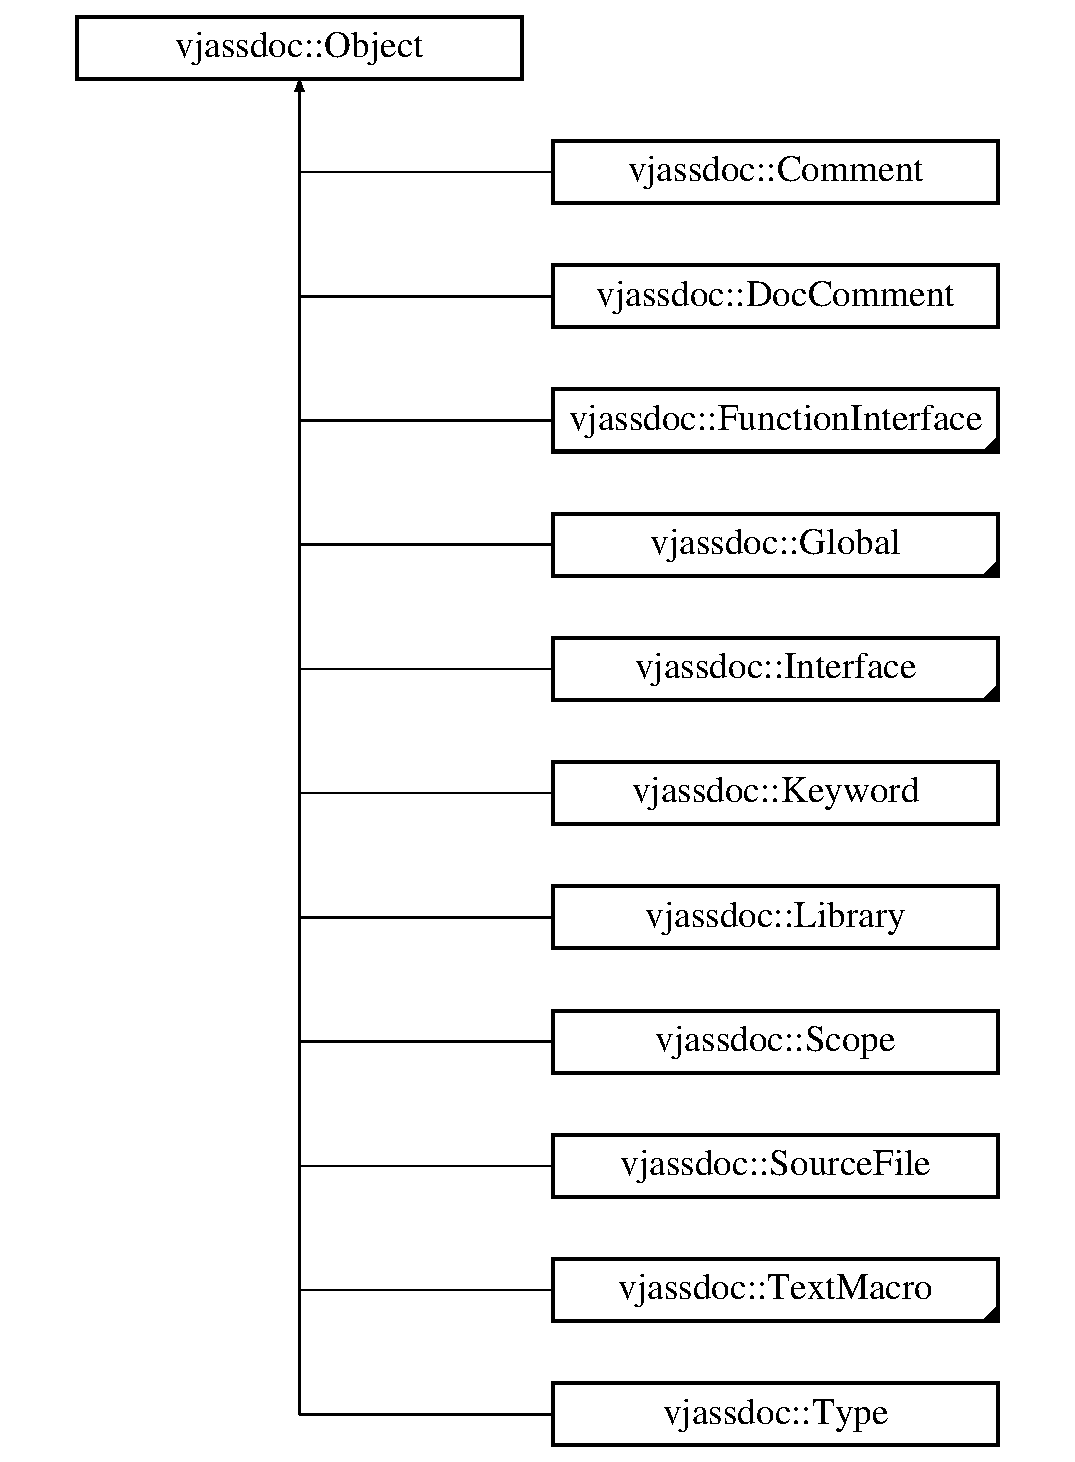
\includegraphics[height=12cm]{classvjassdoc_1_1Object}
\end{center}
\end{figure}
\subsection*{Public Member Functions}
\begin{CompactItemize}
\item 
\hyperlink{classvjassdoc_1_1Object_253d645fca4eb52e3d10226fab1d3673}{Object} (const std::string \&identifier, class \hyperlink{classvjassdoc_1_1SourceFile}{SourceFile} $\ast$sourceFile, unsigned int line, class \hyperlink{classvjassdoc_1_1DocComment}{DocComment} $\ast$docComment)
\item 
\hyperlink{classvjassdoc_1_1Object_2e185664aec8264f2fe55500768dc77f}{Object} (std::vector$<$ const unsigned char $\ast$ $>$ \&columnVector)
\item 
virtual \hyperlink{classvjassdoc_1_1Object_ee368858fe1d3723b95600c12a474b38}{$\sim$Object} ()
\item 
virtual void \hyperlink{classvjassdoc_1_1Object_bd43e77dbe80055f5adda67661dfaca4}{init} ()=0
\item 
virtual void \hyperlink{classvjassdoc_1_1Object_736bbb6719edd8070d8f56c364a2764c}{pageNavigation} (std::ofstream \&file) const =0
\item 
virtual void \hyperlink{classvjassdoc_1_1Object_a0489e38956f3507566b1bc6e3e2c8af}{page} (std::ofstream \&file) const =0
\item 
std::string \hyperlink{classvjassdoc_1_1Object_6007f5c1d887da284a5dffd878ff67d6}{pageLink} () const 
\item 
virtual std::string \hyperlink{classvjassdoc_1_1Object_4e8ebbb0ce5b0bf91ec847b1e4a9f8fc}{sqlStatement} () const 
\item 
unsigned int \hyperlink{classvjassdoc_1_1Object_0eaa0868e7e182a8de1fc4061cd21327}{id} () const 
\item 
void \hyperlink{classvjassdoc_1_1Object_64ce402e1f66de46106dcaaa7f7423f5}{addIdentifier} (const std::string \&identifier)
\item 
std::string \hyperlink{classvjassdoc_1_1Object_c2927d3fd29e7b9ba25a481f6c0bcd75}{identifier} () const 
\item 
class \hyperlink{classvjassdoc_1_1SourceFile}{SourceFile} $\ast$ \hyperlink{classvjassdoc_1_1Object_c09bed4bd1d246d9aa8b96b9317a2b4a}{sourceFile} () const 
\item 
unsigned int \hyperlink{classvjassdoc_1_1Object_e0124e6b7fd1642276274c058b280abf}{line} () const 
\item 
class \hyperlink{classvjassdoc_1_1DocComment}{DocComment} $\ast$ \hyperlink{classvjassdoc_1_1Object_57a2a1b81c481ee49738df29f1f63b2b}{docComment} () const 
\item 
virtual class \hyperlink{classvjassdoc_1_1Object}{Object} $\ast$ \hyperlink{classvjassdoc_1_1Object_b3729c3b063682f94b43a42546c90e96}{container} () const 
\item 
virtual class \hyperlink{classvjassdoc_1_1Scope}{Scope} $\ast$ \hyperlink{classvjassdoc_1_1Object_0738d05b196cc8b9e89d62839d81fc20}{scope} () const 
\item 
virtual class \hyperlink{classvjassdoc_1_1Library}{Library} $\ast$ \hyperlink{classvjassdoc_1_1Object_cc4241505c5bcdd0bbcb08a1b665b3fd}{library} () const 
\end{CompactItemize}
\subsection*{Static Public Member Functions}
\begin{CompactItemize}
\item 
static std::string \hyperlink{classvjassdoc_1_1Object_1e7cc8e9b75c8555f996ecd9af27e446}{objectPageLink} (const class \hyperlink{classvjassdoc_1_1Object}{Object} $\ast$object, const std::string \&identifier=\char`\"{}-\char`\"{})
\item 
static std::string \hyperlink{classvjassdoc_1_1Object_0f115e83ce406e04b8ff20bacfb4acab}{objectLink} (const class \hyperlink{classvjassdoc_1_1Object}{Object} $\ast$object, const std::string \&identifier=\char`\"{}-\char`\"{})
\item 
static int \hyperlink{classvjassdoc_1_1Object_7da4025933552d2e896a8ea2534b3324}{objectId} (const class \hyperlink{classvjassdoc_1_1Object}{Object} $\ast$object)
\item 
static void \hyperlink{classvjassdoc_1_1Object_8edf943aa716a2da74d4f9f2c13e001b}{setMaxIds} (int maxIds)
\item 
static std::string \hyperlink{classvjassdoc_1_1Object_402f48ed33d2c82c1bccda774767ded3}{sqlFilteredString} (const std::string \&usedString)
\item 
static std::string \hyperlink{classvjassdoc_1_1Object_b229c2eb3c0c7d1e86d789986bffe3f1}{sqlTableHeader} (const std::string \&tableName, const std::string \&entries)
\end{CompactItemize}
\subsection*{Protected Member Functions}
\begin{CompactItemize}
\item 
void \hyperlink{classvjassdoc_1_1Object_3b69e9dd345029eef00edd37b4b171df}{setIdentifier} (const std::string \&identifier)
\item 
std::string \hyperlink{classvjassdoc_1_1Object_6ccc2dac8089947b3ad04b306ea700e8}{anchor} () const 
\item 
class \hyperlink{classvjassdoc_1_1Object}{Object} $\ast$ \hyperlink{classvjassdoc_1_1Object_7ec73267fcaaa923333318c63de594da}{searchObjectInList} (const std::string \&identifier, const enum \hyperlink{classvjassdoc_1_1Parser_4ef39527519272daf05a22b5276062ad}{Parser::List} \&list, enum \hyperlink{classvjassdoc_1_1Parser_ed659a05a08c7db4e2d233d133efdfda}{Parser::SearchMode} searchMode=Parser::Unspecified)
\item 
class \hyperlink{classvjassdoc_1_1Object}{Object} $\ast$ \hyperlink{classvjassdoc_1_1Object_4204a70565df779213ae78612560d42e}{findValue} (class \hyperlink{classvjassdoc_1_1Object}{Object} $\ast$type, std::string \&valueExpression)
\end{CompactItemize}
\subsection*{Static Protected Member Functions}
\begin{CompactItemize}
\item 
static bool \hyperlink{classvjassdoc_1_1Object_e9ed6f9d16334a979405a9f2efab2239}{hasToSearchValueObject} (class \hyperlink{classvjassdoc_1_1Object}{Object} $\ast$type, const std::string \&expression)
\item 
static std::string \hyperlink{classvjassdoc_1_1Object_6715790d5be823157b8cf21d181b3450}{showBooleanProperty} (const bool \&property)
\end{CompactItemize}
\subsection*{Protected Attributes}
\begin{CompactItemize}
\item 
class \hyperlink{classvjassdoc_1_1Object}{Object} $\ast$ \hyperlink{classvjassdoc_1_1Object_c14bc17d0da694e343812eed35883859}{m\_\-container}
\item 
class \hyperlink{classvjassdoc_1_1Scope}{Scope} $\ast$ \hyperlink{classvjassdoc_1_1Object_e807f9d1a84a2708976d07b21a17cf81}{m\_\-scope}
\item 
class \hyperlink{classvjassdoc_1_1Library}{Library} $\ast$ \hyperlink{classvjassdoc_1_1Object_90d88574b7a542deb45e65a9242b345a}{m\_\-library}
\end{CompactItemize}
\subsection*{Classes}
\begin{CompactItemize}
\item 
struct \hyperlink{structvjassdoc_1_1Object_1_1AlphabeticalComparator}{AlphabeticalComparator}
\item 
struct \hyperlink{structvjassdoc_1_1Object_1_1IsInContainer}{IsInContainer}
\item 
struct \hyperlink{structvjassdoc_1_1Object_1_1IsInLibrary}{IsInLibrary}
\item 
struct \hyperlink{structvjassdoc_1_1Object_1_1IsInScope}{IsInScope}
\end{CompactItemize}


\subsection{Constructor \& Destructor Documentation}
\hypertarget{classvjassdoc_1_1Object_253d645fca4eb52e3d10226fab1d3673}{
\index{vjassdoc::Object@{vjassdoc::Object}!Object@{Object}}
\index{Object@{Object}!vjassdoc::Object@{vjassdoc::Object}}
\subsubsection{\setlength{\rightskip}{0pt plus 5cm}vjassdoc::Object::Object (const std::string \& {\em identifier}, class {\bf SourceFile} $\ast$ {\em sourceFile}, unsigned int {\em line}, class {\bf DocComment} $\ast$ {\em docComment})}}
\label{classvjassdoc_1_1Object_253d645fca4eb52e3d10226fab1d3673}


\hypertarget{classvjassdoc_1_1Object_2e185664aec8264f2fe55500768dc77f}{
\index{vjassdoc::Object@{vjassdoc::Object}!Object@{Object}}
\index{Object@{Object}!vjassdoc::Object@{vjassdoc::Object}}
\subsubsection{\setlength{\rightskip}{0pt plus 5cm}vjassdoc::Object::Object (std::vector$<$ const unsigned char $\ast$ $>$ \& {\em columnVector})}}
\label{classvjassdoc_1_1Object_2e185664aec8264f2fe55500768dc77f}


\hypertarget{classvjassdoc_1_1Object_ee368858fe1d3723b95600c12a474b38}{
\index{vjassdoc::Object@{vjassdoc::Object}!$\sim$Object@{$\sim$Object}}
\index{$\sim$Object@{$\sim$Object}!vjassdoc::Object@{vjassdoc::Object}}
\subsubsection{\setlength{\rightskip}{0pt plus 5cm}vjassdoc::Object::$\sim$Object ()\hspace{0.3cm}{\tt  \mbox{[}virtual\mbox{]}}}}
\label{classvjassdoc_1_1Object_ee368858fe1d3723b95600c12a474b38}




\subsection{Member Function Documentation}
\hypertarget{classvjassdoc_1_1Object_1e7cc8e9b75c8555f996ecd9af27e446}{
\index{vjassdoc::Object@{vjassdoc::Object}!objectPageLink@{objectPageLink}}
\index{objectPageLink@{objectPageLink}!vjassdoc::Object@{vjassdoc::Object}}
\subsubsection{\setlength{\rightskip}{0pt plus 5cm}std::string vjassdoc::Object::objectPageLink (const class {\bf Object} $\ast$ {\em object}, const std::string \& {\em identifier} = {\tt \char`\"{}-\char`\"{}})\hspace{0.3cm}{\tt  \mbox{[}inline, static\mbox{]}}}}
\label{classvjassdoc_1_1Object_1e7cc8e9b75c8555f996ecd9af27e446}


\hypertarget{classvjassdoc_1_1Object_0f115e83ce406e04b8ff20bacfb4acab}{
\index{vjassdoc::Object@{vjassdoc::Object}!objectLink@{objectLink}}
\index{objectLink@{objectLink}!vjassdoc::Object@{vjassdoc::Object}}
\subsubsection{\setlength{\rightskip}{0pt plus 5cm}std::string vjassdoc::Object::objectLink (const class {\bf Object} $\ast$ {\em object}, const std::string \& {\em identifier} = {\tt \char`\"{}-\char`\"{}})\hspace{0.3cm}{\tt  \mbox{[}inline, static\mbox{]}}}}
\label{classvjassdoc_1_1Object_0f115e83ce406e04b8ff20bacfb4acab}


\hypertarget{classvjassdoc_1_1Object_7da4025933552d2e896a8ea2534b3324}{
\index{vjassdoc::Object@{vjassdoc::Object}!objectId@{objectId}}
\index{objectId@{objectId}!vjassdoc::Object@{vjassdoc::Object}}
\subsubsection{\setlength{\rightskip}{0pt plus 5cm}int vjassdoc::Object::objectId (const class {\bf Object} $\ast$ {\em object})\hspace{0.3cm}{\tt  \mbox{[}inline, static\mbox{]}}}}
\label{classvjassdoc_1_1Object_7da4025933552d2e896a8ea2534b3324}


\hypertarget{classvjassdoc_1_1Object_8edf943aa716a2da74d4f9f2c13e001b}{
\index{vjassdoc::Object@{vjassdoc::Object}!setMaxIds@{setMaxIds}}
\index{setMaxIds@{setMaxIds}!vjassdoc::Object@{vjassdoc::Object}}
\subsubsection{\setlength{\rightskip}{0pt plus 5cm}void vjassdoc::Object::setMaxIds (int {\em maxIds})\hspace{0.3cm}{\tt  \mbox{[}inline, static\mbox{]}}}}
\label{classvjassdoc_1_1Object_8edf943aa716a2da74d4f9f2c13e001b}


\hypertarget{classvjassdoc_1_1Object_402f48ed33d2c82c1bccda774767ded3}{
\index{vjassdoc::Object@{vjassdoc::Object}!sqlFilteredString@{sqlFilteredString}}
\index{sqlFilteredString@{sqlFilteredString}!vjassdoc::Object@{vjassdoc::Object}}
\subsubsection{\setlength{\rightskip}{0pt plus 5cm}std::string vjassdoc::Object::sqlFilteredString (const std::string \& {\em usedString})\hspace{0.3cm}{\tt  \mbox{[}static\mbox{]}}}}
\label{classvjassdoc_1_1Object_402f48ed33d2c82c1bccda774767ded3}


\hypertarget{classvjassdoc_1_1Object_b229c2eb3c0c7d1e86d789986bffe3f1}{
\index{vjassdoc::Object@{vjassdoc::Object}!sqlTableHeader@{sqlTableHeader}}
\index{sqlTableHeader@{sqlTableHeader}!vjassdoc::Object@{vjassdoc::Object}}
\subsubsection{\setlength{\rightskip}{0pt plus 5cm}std::string vjassdoc::Object::sqlTableHeader (const std::string \& {\em tableName}, const std::string \& {\em entries})\hspace{0.3cm}{\tt  \mbox{[}static\mbox{]}}}}
\label{classvjassdoc_1_1Object_b229c2eb3c0c7d1e86d789986bffe3f1}


\begin{Desc}
\item[\hyperlink{todo__todo000005}{Todo}]This function should be used to distribute all table header creations to their classes. \end{Desc}
\hypertarget{classvjassdoc_1_1Object_bd43e77dbe80055f5adda67661dfaca4}{
\index{vjassdoc::Object@{vjassdoc::Object}!init@{init}}
\index{init@{init}!vjassdoc::Object@{vjassdoc::Object}}
\subsubsection{\setlength{\rightskip}{0pt plus 5cm}virtual void vjassdoc::Object::init ()\hspace{0.3cm}{\tt  \mbox{[}pure virtual\mbox{]}}}}
\label{classvjassdoc_1_1Object_bd43e77dbe80055f5adda67661dfaca4}




Implemented in \hyperlink{classvjassdoc_1_1Comment_07ad51bf42ce397832b77eb96379c054}{vjassdoc::Comment}, \hyperlink{classvjassdoc_1_1DocComment_46ada773166611c9be898f74e0eb2315}{vjassdoc::DocComment}, \hyperlink{classvjassdoc_1_1Function_031d74f7df7c29afb36626fd335b2037}{vjassdoc::Function}, \hyperlink{classvjassdoc_1_1FunctionInterface_3b988163d8012beac222b27f80484242}{vjassdoc::FunctionInterface}, \hyperlink{classvjassdoc_1_1Global_9e6189cfd577f0453988e8c8c6eec04d}{vjassdoc::Global}, \hyperlink{classvjassdoc_1_1Interface_e10d2a4a6acf44897145bf76675b9da1}{vjassdoc::Interface}, \hyperlink{classvjassdoc_1_1Keyword_0aeec733c7c55ff51c8b1ba58af18ed9}{vjassdoc::Keyword}, \hyperlink{classvjassdoc_1_1Library_d1bbc6153d45c040be60419a6708bd7d}{vjassdoc::Library}, \hyperlink{classvjassdoc_1_1Member_eccac74ca5ea37e82d322c20b5aa2efc}{vjassdoc::Member}, \hyperlink{classvjassdoc_1_1Method_cd115b1b9a459752e6613925be8e9daf}{vjassdoc::Method}, \hyperlink{classvjassdoc_1_1Scope_fb5915ecd0cabc72508e7b7a09f0ef5c}{vjassdoc::Scope}, \hyperlink{classvjassdoc_1_1SourceFile_e2aa3f034bbb18de023ce9a21dfa78d1}{vjassdoc::SourceFile}, \hyperlink{classvjassdoc_1_1Struct_39dc86da31e526f3a6eb3b6e442156bb}{vjassdoc::Struct}, \hyperlink{classvjassdoc_1_1TextMacro_816bdd2b838a4f1148ea17e5723e8577}{vjassdoc::TextMacro}, \hyperlink{classvjassdoc_1_1TextMacroInstance_e60b03ce172f8eefde2cdcc31533ee2d}{vjassdoc::TextMacroInstance}, and \hyperlink{classvjassdoc_1_1Type_d4cadc76713790490c55be0bd0af1a1d}{vjassdoc::Type}.\hypertarget{classvjassdoc_1_1Object_736bbb6719edd8070d8f56c364a2764c}{
\index{vjassdoc::Object@{vjassdoc::Object}!pageNavigation@{pageNavigation}}
\index{pageNavigation@{pageNavigation}!vjassdoc::Object@{vjassdoc::Object}}
\subsubsection{\setlength{\rightskip}{0pt plus 5cm}virtual void vjassdoc::Object::pageNavigation (std::ofstream \& {\em file}) const\hspace{0.3cm}{\tt  \mbox{[}pure virtual\mbox{]}}}}
\label{classvjassdoc_1_1Object_736bbb6719edd8070d8f56c364a2764c}




Implemented in \hyperlink{classvjassdoc_1_1Comment_4bcb5f83071ad7954b922fdaf8e0ea8e}{vjassdoc::Comment}, \hyperlink{classvjassdoc_1_1DocComment_2a0b017c17c8a20679b2052b87a74c15}{vjassdoc::DocComment}, \hyperlink{classvjassdoc_1_1Function_b0776a1e111d7fcefbbcecd92f210a48}{vjassdoc::Function}, \hyperlink{classvjassdoc_1_1FunctionInterface_90bd64ed95596db63699df15aa35216e}{vjassdoc::FunctionInterface}, \hyperlink{classvjassdoc_1_1Global_8c5209b5652d3633feb1d7fab796b439}{vjassdoc::Global}, \hyperlink{classvjassdoc_1_1Interface_f0acc07a23eb46eb9f065fb47d55f1a5}{vjassdoc::Interface}, \hyperlink{classvjassdoc_1_1Keyword_c8950d4ece99a58cc664daf5f652f37c}{vjassdoc::Keyword}, \hyperlink{classvjassdoc_1_1Library_782d6d0f5d58756924f0ab413821967a}{vjassdoc::Library}, \hyperlink{classvjassdoc_1_1Member_fa8e020175714b1f03a3696cc935941f}{vjassdoc::Member}, \hyperlink{classvjassdoc_1_1Method_d5d61124a7d28d7e4680cc0df6cc5deb}{vjassdoc::Method}, \hyperlink{classvjassdoc_1_1Scope_3fac1b4e0201e20463acfc5f0f0e93b8}{vjassdoc::Scope}, \hyperlink{classvjassdoc_1_1SourceFile_b365551c64c03553e8fb1a31d83edaea}{vjassdoc::SourceFile}, \hyperlink{classvjassdoc_1_1Struct_c415c5b26f7385a990339dfbfbbca5dc}{vjassdoc::Struct}, \hyperlink{classvjassdoc_1_1TextMacro_d3ad5fe5300492db3d1aaf250d9b2a4b}{vjassdoc::TextMacro}, \hyperlink{classvjassdoc_1_1TextMacroInstance_2bc8e5c94f5a74795d0c2d8137522d89}{vjassdoc::TextMacroInstance}, and \hyperlink{classvjassdoc_1_1Type_bc514be419f91658df10d742c6999e47}{vjassdoc::Type}.\hypertarget{classvjassdoc_1_1Object_a0489e38956f3507566b1bc6e3e2c8af}{
\index{vjassdoc::Object@{vjassdoc::Object}!page@{page}}
\index{page@{page}!vjassdoc::Object@{vjassdoc::Object}}
\subsubsection{\setlength{\rightskip}{0pt plus 5cm}virtual void vjassdoc::Object::page (std::ofstream \& {\em file}) const\hspace{0.3cm}{\tt  \mbox{[}pure virtual\mbox{]}}}}
\label{classvjassdoc_1_1Object_a0489e38956f3507566b1bc6e3e2c8af}




Implemented in \hyperlink{classvjassdoc_1_1Comment_d7b59c02557b961deb2f470b180bab7a}{vjassdoc::Comment}, \hyperlink{classvjassdoc_1_1DocComment_79dd94421713887af6028f49736d895d}{vjassdoc::DocComment}, \hyperlink{classvjassdoc_1_1Function_7f32865b4c3f9f4c4e6379a437f5bdfe}{vjassdoc::Function}, \hyperlink{classvjassdoc_1_1FunctionInterface_3f5c67bb77822e08047b327f244ec364}{vjassdoc::FunctionInterface}, \hyperlink{classvjassdoc_1_1Global_1b8fefe2b9c895c122a822bac0383f1b}{vjassdoc::Global}, \hyperlink{classvjassdoc_1_1Interface_79ed4ee7fd055e3b53fdb9b14749fa0f}{vjassdoc::Interface}, \hyperlink{classvjassdoc_1_1Keyword_207c989cefeeb0857adb76aa5d7bd842}{vjassdoc::Keyword}, \hyperlink{classvjassdoc_1_1Library_b49718631812ed3a5bcfe0a5bdf7595e}{vjassdoc::Library}, \hyperlink{classvjassdoc_1_1Member_2bd66eba1882dfb2dcbf2552b42d1346}{vjassdoc::Member}, \hyperlink{classvjassdoc_1_1Method_564b24f8b05185ac9399dd36a9b0ad1a}{vjassdoc::Method}, \hyperlink{classvjassdoc_1_1Scope_2a37c9d88da6a8c7c95d4f0e5b88ccbb}{vjassdoc::Scope}, \hyperlink{classvjassdoc_1_1SourceFile_0a4aed2c620f52f3cb114843f674b31c}{vjassdoc::SourceFile}, \hyperlink{classvjassdoc_1_1Struct_bd918c5a1ec7defe1849f4b4e61523f2}{vjassdoc::Struct}, \hyperlink{classvjassdoc_1_1TextMacro_3336cdf9ad953dbd44b38fb14a2f73fa}{vjassdoc::TextMacro}, \hyperlink{classvjassdoc_1_1TextMacroInstance_4785937fa62c12f3586276a2d5dcbe52}{vjassdoc::TextMacroInstance}, and \hyperlink{classvjassdoc_1_1Type_aa7a3044fc74587aa8800b1d67b18930}{vjassdoc::Type}.\hypertarget{classvjassdoc_1_1Object_6007f5c1d887da284a5dffd878ff67d6}{
\index{vjassdoc::Object@{vjassdoc::Object}!pageLink@{pageLink}}
\index{pageLink@{pageLink}!vjassdoc::Object@{vjassdoc::Object}}
\subsubsection{\setlength{\rightskip}{0pt plus 5cm}std::string vjassdoc::Object::pageLink () const\hspace{0.3cm}{\tt  \mbox{[}inline\mbox{]}}}}
\label{classvjassdoc_1_1Object_6007f5c1d887da284a5dffd878ff67d6}


\hypertarget{classvjassdoc_1_1Object_4e8ebbb0ce5b0bf91ec847b1e4a9f8fc}{
\index{vjassdoc::Object@{vjassdoc::Object}!sqlStatement@{sqlStatement}}
\index{sqlStatement@{sqlStatement}!vjassdoc::Object@{vjassdoc::Object}}
\subsubsection{\setlength{\rightskip}{0pt plus 5cm}std::string vjassdoc::Object::sqlStatement () const\hspace{0.3cm}{\tt  \mbox{[}virtual\mbox{]}}}}
\label{classvjassdoc_1_1Object_4e8ebbb0ce5b0bf91ec847b1e4a9f8fc}




Reimplemented in \hyperlink{classvjassdoc_1_1DocComment_d50177b6a9bd805ebe1ef76b8607242e}{vjassdoc::DocComment}, \hyperlink{classvjassdoc_1_1Function_7e4a84e1bb86ade42e6a95d81d8092a7}{vjassdoc::Function}, \hyperlink{classvjassdoc_1_1FunctionInterface_20b33401bc90587128da6bae1c6986d8}{vjassdoc::FunctionInterface}, \hyperlink{classvjassdoc_1_1Global_4e9a8ea0c8bc34f6980d31676e497531}{vjassdoc::Global}, \hyperlink{classvjassdoc_1_1Interface_93fbe7323df0502111e576c08376b726}{vjassdoc::Interface}, \hyperlink{classvjassdoc_1_1Keyword_b2d197337624e89955564ac684bfd5ad}{vjassdoc::Keyword}, \hyperlink{classvjassdoc_1_1Library_21dd8d48803fa96b2b22cb9846c9b915}{vjassdoc::Library}, \hyperlink{classvjassdoc_1_1Member_ad210521f998bd4c8be5f8af3ae74cf1}{vjassdoc::Member}, \hyperlink{classvjassdoc_1_1Method_0a9c4b3b9cb2043eb1454ae72bbfe04f}{vjassdoc::Method}, \hyperlink{classvjassdoc_1_1Scope_634ae4bc06389b21ef8612795d4a910f}{vjassdoc::Scope}, \hyperlink{classvjassdoc_1_1SourceFile_cda6410687f71928eafac94a635c4250}{vjassdoc::SourceFile}, \hyperlink{classvjassdoc_1_1Struct_227d826acdbbe1702941634c90ab7e4e}{vjassdoc::Struct}, \hyperlink{classvjassdoc_1_1TextMacro_e46c88feedc6197fbbae48de17f07366}{vjassdoc::TextMacro}, \hyperlink{classvjassdoc_1_1TextMacroInstance_7659e7ac5ff7547dfc526a4a7ff152b5}{vjassdoc::TextMacroInstance}, and \hyperlink{classvjassdoc_1_1Type_22741189ccde7fa7bc63abdeaf256c92}{vjassdoc::Type}.\hypertarget{classvjassdoc_1_1Object_0eaa0868e7e182a8de1fc4061cd21327}{
\index{vjassdoc::Object@{vjassdoc::Object}!id@{id}}
\index{id@{id}!vjassdoc::Object@{vjassdoc::Object}}
\subsubsection{\setlength{\rightskip}{0pt plus 5cm}unsigned int vjassdoc::Object::id () const\hspace{0.3cm}{\tt  \mbox{[}inline\mbox{]}}}}
\label{classvjassdoc_1_1Object_0eaa0868e7e182a8de1fc4061cd21327}


\hypertarget{classvjassdoc_1_1Object_64ce402e1f66de46106dcaaa7f7423f5}{
\index{vjassdoc::Object@{vjassdoc::Object}!addIdentifier@{addIdentifier}}
\index{addIdentifier@{addIdentifier}!vjassdoc::Object@{vjassdoc::Object}}
\subsubsection{\setlength{\rightskip}{0pt plus 5cm}void vjassdoc::Object::addIdentifier (const std::string \& {\em identifier})\hspace{0.3cm}{\tt  \mbox{[}inline\mbox{]}}}}
\label{classvjassdoc_1_1Object_64ce402e1f66de46106dcaaa7f7423f5}


\hypertarget{classvjassdoc_1_1Object_c2927d3fd29e7b9ba25a481f6c0bcd75}{
\index{vjassdoc::Object@{vjassdoc::Object}!identifier@{identifier}}
\index{identifier@{identifier}!vjassdoc::Object@{vjassdoc::Object}}
\subsubsection{\setlength{\rightskip}{0pt plus 5cm}std::string vjassdoc::Object::identifier () const\hspace{0.3cm}{\tt  \mbox{[}inline\mbox{]}}}}
\label{classvjassdoc_1_1Object_c2927d3fd29e7b9ba25a481f6c0bcd75}


\hypertarget{classvjassdoc_1_1Object_c09bed4bd1d246d9aa8b96b9317a2b4a}{
\index{vjassdoc::Object@{vjassdoc::Object}!sourceFile@{sourceFile}}
\index{sourceFile@{sourceFile}!vjassdoc::Object@{vjassdoc::Object}}
\subsubsection{\setlength{\rightskip}{0pt plus 5cm}class {\bf SourceFile} $\ast$ vjassdoc::Object::sourceFile () const\hspace{0.3cm}{\tt  \mbox{[}inline\mbox{]}}}}
\label{classvjassdoc_1_1Object_c09bed4bd1d246d9aa8b96b9317a2b4a}


\hypertarget{classvjassdoc_1_1Object_e0124e6b7fd1642276274c058b280abf}{
\index{vjassdoc::Object@{vjassdoc::Object}!line@{line}}
\index{line@{line}!vjassdoc::Object@{vjassdoc::Object}}
\subsubsection{\setlength{\rightskip}{0pt plus 5cm}unsigned int vjassdoc::Object::line () const\hspace{0.3cm}{\tt  \mbox{[}inline\mbox{]}}}}
\label{classvjassdoc_1_1Object_e0124e6b7fd1642276274c058b280abf}


\hypertarget{classvjassdoc_1_1Object_57a2a1b81c481ee49738df29f1f63b2b}{
\index{vjassdoc::Object@{vjassdoc::Object}!docComment@{docComment}}
\index{docComment@{docComment}!vjassdoc::Object@{vjassdoc::Object}}
\subsubsection{\setlength{\rightskip}{0pt plus 5cm}class {\bf DocComment} $\ast$ vjassdoc::Object::docComment () const\hspace{0.3cm}{\tt  \mbox{[}inline\mbox{]}}}}
\label{classvjassdoc_1_1Object_57a2a1b81c481ee49738df29f1f63b2b}


\hypertarget{classvjassdoc_1_1Object_b3729c3b063682f94b43a42546c90e96}{
\index{vjassdoc::Object@{vjassdoc::Object}!container@{container}}
\index{container@{container}!vjassdoc::Object@{vjassdoc::Object}}
\subsubsection{\setlength{\rightskip}{0pt plus 5cm}class {\bf Object} $\ast$ vjassdoc::Object::container () const\hspace{0.3cm}{\tt  \mbox{[}virtual\mbox{]}}}}
\label{classvjassdoc_1_1Object_b3729c3b063682f94b43a42546c90e96}




Reimplemented in \hyperlink{classvjassdoc_1_1Member_313ed6d74338700b34409ccad8dc5360}{vjassdoc::Member}, and \hyperlink{classvjassdoc_1_1Method_647eb53622d1ef78100a97ef9eac9fe3}{vjassdoc::Method}.\hypertarget{classvjassdoc_1_1Object_0738d05b196cc8b9e89d62839d81fc20}{
\index{vjassdoc::Object@{vjassdoc::Object}!scope@{scope}}
\index{scope@{scope}!vjassdoc::Object@{vjassdoc::Object}}
\subsubsection{\setlength{\rightskip}{0pt plus 5cm}class {\bf Scope} $\ast$ vjassdoc::Object::scope () const\hspace{0.3cm}{\tt  \mbox{[}virtual\mbox{]}}}}
\label{classvjassdoc_1_1Object_0738d05b196cc8b9e89d62839d81fc20}




Reimplemented in \hyperlink{classvjassdoc_1_1FunctionInterface_3d298257fab6e122f44f07225ee3ab63}{vjassdoc::FunctionInterface}, \hyperlink{classvjassdoc_1_1Global_239f8dbfff5e8ed7580d6ba9aadd5f55}{vjassdoc::Global}, \hyperlink{classvjassdoc_1_1Interface_407dbdb20eabf2e9f08bf7c459910335}{vjassdoc::Interface}, and \hyperlink{classvjassdoc_1_1Keyword_5524a7a3029192c2c460a1914cce63e3}{vjassdoc::Keyword}.\hypertarget{classvjassdoc_1_1Object_cc4241505c5bcdd0bbcb08a1b665b3fd}{
\index{vjassdoc::Object@{vjassdoc::Object}!library@{library}}
\index{library@{library}!vjassdoc::Object@{vjassdoc::Object}}
\subsubsection{\setlength{\rightskip}{0pt plus 5cm}class {\bf Library} $\ast$ vjassdoc::Object::library () const\hspace{0.3cm}{\tt  \mbox{[}virtual\mbox{]}}}}
\label{classvjassdoc_1_1Object_cc4241505c5bcdd0bbcb08a1b665b3fd}




Reimplemented in \hyperlink{classvjassdoc_1_1FunctionInterface_c9519495c94b07101fa5e0739775759e}{vjassdoc::FunctionInterface}, \hyperlink{classvjassdoc_1_1Global_cbf7be8310f31bd7dc142b290020b4a9}{vjassdoc::Global}, \hyperlink{classvjassdoc_1_1Interface_69ae9cd3e06f91fc2c33ebd6f1b425fe}{vjassdoc::Interface}, \hyperlink{classvjassdoc_1_1Keyword_9496b5c2a1eedee46d27dd166608b12f}{vjassdoc::Keyword}, and \hyperlink{classvjassdoc_1_1Scope_4d9d486897a1960cff057ab88a43fb15}{vjassdoc::Scope}.\hypertarget{classvjassdoc_1_1Object_e9ed6f9d16334a979405a9f2efab2239}{
\index{vjassdoc::Object@{vjassdoc::Object}!hasToSearchValueObject@{hasToSearchValueObject}}
\index{hasToSearchValueObject@{hasToSearchValueObject}!vjassdoc::Object@{vjassdoc::Object}}
\subsubsection{\setlength{\rightskip}{0pt plus 5cm}bool vjassdoc::Object::hasToSearchValueObject (class {\bf Object} $\ast$ {\em type}, const std::string \& {\em expression})\hspace{0.3cm}{\tt  \mbox{[}static, protected\mbox{]}}}}
\label{classvjassdoc_1_1Object_e9ed6f9d16334a979405a9f2efab2239}


Checks if the value \begin{Desc}
\item[Parameters:]
\begin{description}
\item[{\em expression}]which has type \item[{\em type}]is a literal or not. If it is no literal method will return true. \end{description}
\end{Desc}


\begin{Desc}
\item[\hyperlink{todo__todo000004}{Todo}]Code type == null?! \end{Desc}
\hypertarget{classvjassdoc_1_1Object_6715790d5be823157b8cf21d181b3450}{
\index{vjassdoc::Object@{vjassdoc::Object}!showBooleanProperty@{showBooleanProperty}}
\index{showBooleanProperty@{showBooleanProperty}!vjassdoc::Object@{vjassdoc::Object}}
\subsubsection{\setlength{\rightskip}{0pt plus 5cm}std::string vjassdoc::Object::showBooleanProperty (const bool \& {\em property})\hspace{0.3cm}{\tt  \mbox{[}inline, static, protected\mbox{]}}}}
\label{classvjassdoc_1_1Object_6715790d5be823157b8cf21d181b3450}


Shows a boolean value. This method has been written for showing boolean members of classes in a HTML file. Instead of 0 and 1 it returns the strings 'No' and 'Yes' in the local language. \hypertarget{classvjassdoc_1_1Object_3b69e9dd345029eef00edd37b4b171df}{
\index{vjassdoc::Object@{vjassdoc::Object}!setIdentifier@{setIdentifier}}
\index{setIdentifier@{setIdentifier}!vjassdoc::Object@{vjassdoc::Object}}
\subsubsection{\setlength{\rightskip}{0pt plus 5cm}void vjassdoc::Object::setIdentifier (const std::string \& {\em identifier})\hspace{0.3cm}{\tt  \mbox{[}inline, protected\mbox{]}}}}
\label{classvjassdoc_1_1Object_3b69e9dd345029eef00edd37b4b171df}


\hypertarget{classvjassdoc_1_1Object_6ccc2dac8089947b3ad04b306ea700e8}{
\index{vjassdoc::Object@{vjassdoc::Object}!anchor@{anchor}}
\index{anchor@{anchor}!vjassdoc::Object@{vjassdoc::Object}}
\subsubsection{\setlength{\rightskip}{0pt plus 5cm}std::string vjassdoc::Object::anchor () const\hspace{0.3cm}{\tt  \mbox{[}inline, protected\mbox{]}}}}
\label{classvjassdoc_1_1Object_6ccc2dac8089947b3ad04b306ea700e8}


\hypertarget{classvjassdoc_1_1Object_7ec73267fcaaa923333318c63de594da}{
\index{vjassdoc::Object@{vjassdoc::Object}!searchObjectInList@{searchObjectInList}}
\index{searchObjectInList@{searchObjectInList}!vjassdoc::Object@{vjassdoc::Object}}
\subsubsection{\setlength{\rightskip}{0pt plus 5cm}class {\bf Object} $\ast$ vjassdoc::Object::searchObjectInList (const std::string \& {\em identifier}, const enum {\bf Parser::List} \& {\em list}, enum {\bf Parser::SearchMode} {\em searchMode} = {\tt Parser::Unspecified})\hspace{0.3cm}{\tt  \mbox{[}inline, protected\mbox{]}}}}
\label{classvjassdoc_1_1Object_7ec73267fcaaa923333318c63de594da}


\hypertarget{classvjassdoc_1_1Object_4204a70565df779213ae78612560d42e}{
\index{vjassdoc::Object@{vjassdoc::Object}!findValue@{findValue}}
\index{findValue@{findValue}!vjassdoc::Object@{vjassdoc::Object}}
\subsubsection{\setlength{\rightskip}{0pt plus 5cm}class {\bf Object} $\ast$ vjassdoc::Object::findValue (class {\bf Object} $\ast$ {\em type}, std::string \& {\em valueExpression})\hspace{0.3cm}{\tt  \mbox{[}protected\mbox{]}}}}
\label{classvjassdoc_1_1Object_4204a70565df779213ae78612560d42e}


Checks if \begin{Desc}
\item[Parameters:]
\begin{description}
\item[{\em valueExpression}]is a literal or an object. If it's an object (like a global or function call) it will be searched in parser lists. \end{description}
\end{Desc}


\subsection{Member Data Documentation}
\hypertarget{classvjassdoc_1_1Object_c14bc17d0da694e343812eed35883859}{
\index{vjassdoc::Object@{vjassdoc::Object}!m\_\-container@{m\_\-container}}
\index{m\_\-container@{m\_\-container}!vjassdoc::Object@{vjassdoc::Object}}
\subsubsection{\setlength{\rightskip}{0pt plus 5cm}class {\bf Object}$\ast$ {\bf vjassdoc::Object::m\_\-container}\hspace{0.3cm}{\tt  \mbox{[}protected\mbox{]}}}}
\label{classvjassdoc_1_1Object_c14bc17d0da694e343812eed35883859}


\hypertarget{classvjassdoc_1_1Object_e807f9d1a84a2708976d07b21a17cf81}{
\index{vjassdoc::Object@{vjassdoc::Object}!m\_\-scope@{m\_\-scope}}
\index{m\_\-scope@{m\_\-scope}!vjassdoc::Object@{vjassdoc::Object}}
\subsubsection{\setlength{\rightskip}{0pt plus 5cm}class {\bf Scope}$\ast$ {\bf vjassdoc::Object::m\_\-scope}\hspace{0.3cm}{\tt  \mbox{[}protected\mbox{]}}}}
\label{classvjassdoc_1_1Object_e807f9d1a84a2708976d07b21a17cf81}


\hypertarget{classvjassdoc_1_1Object_90d88574b7a542deb45e65a9242b345a}{
\index{vjassdoc::Object@{vjassdoc::Object}!m\_\-library@{m\_\-library}}
\index{m\_\-library@{m\_\-library}!vjassdoc::Object@{vjassdoc::Object}}
\subsubsection{\setlength{\rightskip}{0pt plus 5cm}class {\bf Library}$\ast$ {\bf vjassdoc::Object::m\_\-library}\hspace{0.3cm}{\tt  \mbox{[}protected\mbox{]}}}}
\label{classvjassdoc_1_1Object_90d88574b7a542deb45e65a9242b345a}




The documentation for this class was generated from the following files:\begin{CompactItemize}
\item 
src/\hyperlink{object_8h}{object.h}\item 
src/\hyperlink{object_8cpp}{object.cpp}\end{CompactItemize}

\hypertarget{structvjassdoc_1_1Object_1_1AlphabeticalComparator}{
\section{vjassdoc::Object::AlphabeticalComparator Struct Reference}
\label{structvjassdoc_1_1Object_1_1AlphabeticalComparator}\index{vjassdoc::Object::AlphabeticalComparator@{vjassdoc::Object::AlphabeticalComparator}}
}
{\tt \#include $<$object.h$>$}

\subsection*{Public Member Functions}
\begin{CompactItemize}
\item 
bool \hyperlink{structvjassdoc_1_1Object_1_1AlphabeticalComparator_7bb1d713406baf20c381d24a52ce6445}{operator()} (const class \hyperlink{classvjassdoc_1_1Object}{Object} $\ast$first, const class \hyperlink{classvjassdoc_1_1Object}{Object} $\ast$second) const 
\end{CompactItemize}


\subsection{Member Function Documentation}
\hypertarget{structvjassdoc_1_1Object_1_1AlphabeticalComparator_7bb1d713406baf20c381d24a52ce6445}{
\index{vjassdoc::Object::AlphabeticalComparator@{vjassdoc::Object::AlphabeticalComparator}!operator()@{operator()}}
\index{operator()@{operator()}!vjassdoc::Object::AlphabeticalComparator@{vjassdoc::Object::AlphabeticalComparator}}
\subsubsection{\setlength{\rightskip}{0pt plus 5cm}bool vjassdoc::Object::AlphabeticalComparator::operator() (const class {\bf Object} $\ast$ {\em first}, const class {\bf Object} $\ast$ {\em second}) const\hspace{0.3cm}{\tt  \mbox{[}inline\mbox{]}}}}
\label{structvjassdoc_1_1Object_1_1AlphabeticalComparator_7bb1d713406baf20c381d24a52ce6445}




The documentation for this struct was generated from the following file:\begin{CompactItemize}
\item 
src/\hyperlink{object_8h}{object.h}\end{CompactItemize}

\hypertarget{structvjassdoc_1_1Object_1_1IsInContainer}{
\section{vjassdoc::Object::IsInContainer Struct Reference}
\label{structvjassdoc_1_1Object_1_1IsInContainer}\index{vjassdoc::Object::IsInContainer@{vjassdoc::Object::IsInContainer}}
}
{\tt \#include $<$object.h$>$}

Inheritance diagram for vjassdoc::Object::IsInContainer::\begin{figure}[H]
\begin{center}
\leavevmode
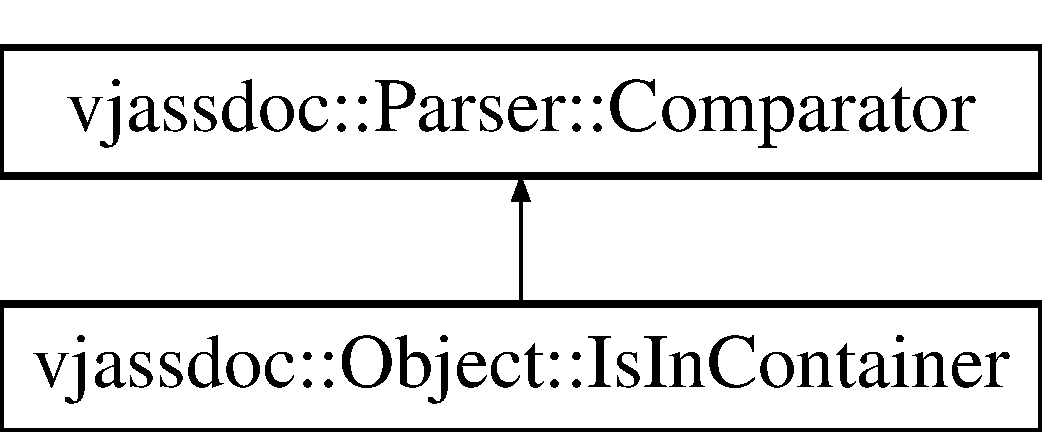
\includegraphics[height=2cm]{structvjassdoc_1_1Object_1_1IsInContainer}
\end{center}
\end{figure}
\subsection*{Public Member Functions}
\begin{CompactItemize}
\item 
virtual bool \hyperlink{structvjassdoc_1_1Object_1_1IsInContainer_390275d3950a824ad1a9ac025964ef64}{operator()} (const class \hyperlink{classvjassdoc_1_1Object}{Object} $\ast$thisObject, const class \hyperlink{classvjassdoc_1_1Object}{Object} $\ast$container) const 
\end{CompactItemize}


\subsection{Member Function Documentation}
\hypertarget{structvjassdoc_1_1Object_1_1IsInContainer_390275d3950a824ad1a9ac025964ef64}{
\index{vjassdoc::Object::IsInContainer@{vjassdoc::Object::IsInContainer}!operator()@{operator()}}
\index{operator()@{operator()}!vjassdoc::Object::IsInContainer@{vjassdoc::Object::IsInContainer}}
\subsubsection{\setlength{\rightskip}{0pt plus 5cm}bool vjassdoc::Object::IsInContainer::operator() (const class {\bf Object} $\ast$ {\em thisObject}, const class {\bf Object} $\ast$ {\em container}) const\hspace{0.3cm}{\tt  \mbox{[}virtual\mbox{]}}}}
\label{structvjassdoc_1_1Object_1_1IsInContainer_390275d3950a824ad1a9ac025964ef64}




Reimplemented from \hyperlink{structvjassdoc_1_1Parser_1_1Comparator_c27d6790182d87751bcf134a0d01481a}{vjassdoc::Parser::Comparator}.

The documentation for this struct was generated from the following files:\begin{CompactItemize}
\item 
src/\hyperlink{object_8h}{object.h}\item 
src/\hyperlink{object_8cpp}{object.cpp}\end{CompactItemize}

\hypertarget{structvjassdoc_1_1Object_1_1IsInLibrary}{
\section{vjassdoc::Object::IsInLibrary Struct Reference}
\label{structvjassdoc_1_1Object_1_1IsInLibrary}\index{vjassdoc::Object::IsInLibrary@{vjassdoc::Object::IsInLibrary}}
}
{\tt \#include $<$object.h$>$}

Inheritance diagram for vjassdoc::Object::IsInLibrary::\begin{figure}[H]
\begin{center}
\leavevmode
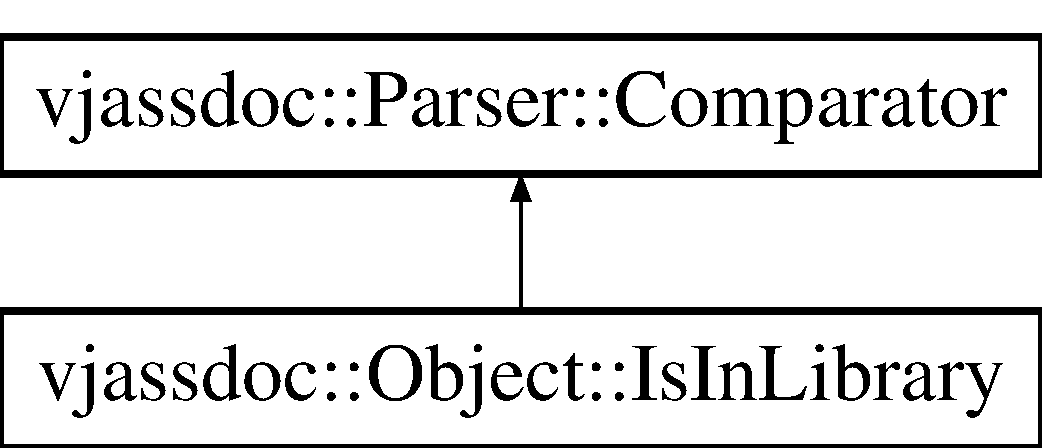
\includegraphics[height=2cm]{structvjassdoc_1_1Object_1_1IsInLibrary}
\end{center}
\end{figure}
\subsection*{Public Member Functions}
\begin{CompactItemize}
\item 
virtual bool \hyperlink{structvjassdoc_1_1Object_1_1IsInLibrary_a1a041f942f665e8f62e30fa2ad3b260}{operator()} (const class \hyperlink{classvjassdoc_1_1Object}{Object} $\ast$thisObject, const class \hyperlink{classvjassdoc_1_1Object}{Object} $\ast$library) const 
\end{CompactItemize}


\subsection{Member Function Documentation}
\hypertarget{structvjassdoc_1_1Object_1_1IsInLibrary_a1a041f942f665e8f62e30fa2ad3b260}{
\index{vjassdoc::Object::IsInLibrary@{vjassdoc::Object::IsInLibrary}!operator()@{operator()}}
\index{operator()@{operator()}!vjassdoc::Object::IsInLibrary@{vjassdoc::Object::IsInLibrary}}
\subsubsection{\setlength{\rightskip}{0pt plus 5cm}bool vjassdoc::Object::IsInLibrary::operator() (const class {\bf Object} $\ast$ {\em thisObject}, const class {\bf Object} $\ast$ {\em library}) const\hspace{0.3cm}{\tt  \mbox{[}virtual\mbox{]}}}}
\label{structvjassdoc_1_1Object_1_1IsInLibrary_a1a041f942f665e8f62e30fa2ad3b260}




Reimplemented from \hyperlink{structvjassdoc_1_1Parser_1_1Comparator_c27d6790182d87751bcf134a0d01481a}{vjassdoc::Parser::Comparator}.

The documentation for this struct was generated from the following files:\begin{CompactItemize}
\item 
src/\hyperlink{object_8h}{object.h}\item 
src/\hyperlink{object_8cpp}{object.cpp}\end{CompactItemize}

\hypertarget{structvjassdoc_1_1Object_1_1IsInScope}{
\section{vjassdoc::Object::IsInScope Struct Reference}
\label{structvjassdoc_1_1Object_1_1IsInScope}\index{vjassdoc::Object::IsInScope@{vjassdoc::Object::IsInScope}}
}
{\tt \#include $<$object.h$>$}

Inheritance diagram for vjassdoc::Object::IsInScope::\begin{figure}[H]
\begin{center}
\leavevmode
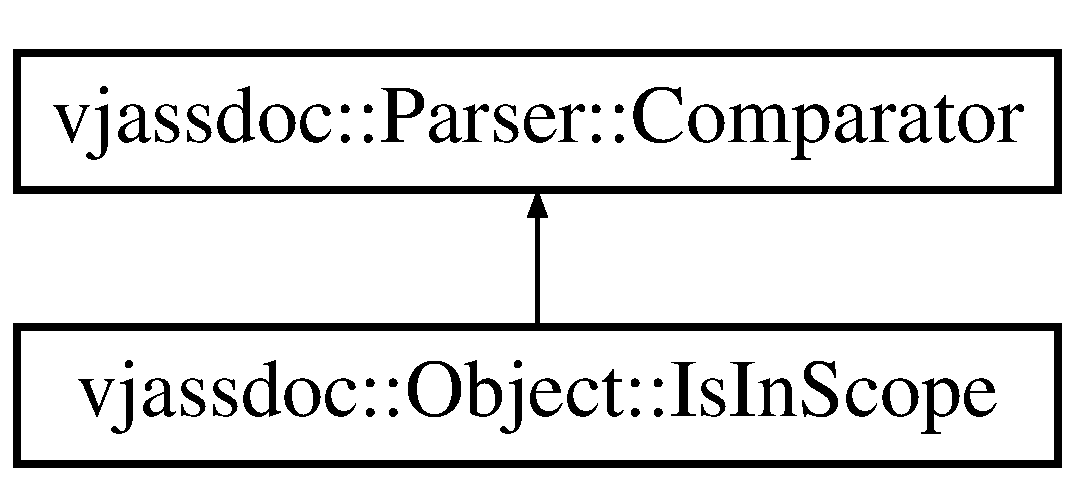
\includegraphics[height=2cm]{structvjassdoc_1_1Object_1_1IsInScope}
\end{center}
\end{figure}
\subsection*{Public Member Functions}
\begin{CompactItemize}
\item 
virtual bool \hyperlink{structvjassdoc_1_1Object_1_1IsInScope_319d4736b3b35681570cc5be477dc5c9}{operator()} (const class \hyperlink{classvjassdoc_1_1Object}{Object} $\ast$thisObject, const class \hyperlink{classvjassdoc_1_1Object}{Object} $\ast$scope) const 
\end{CompactItemize}


\subsection{Member Function Documentation}
\hypertarget{structvjassdoc_1_1Object_1_1IsInScope_319d4736b3b35681570cc5be477dc5c9}{
\index{vjassdoc::Object::IsInScope@{vjassdoc::Object::IsInScope}!operator()@{operator()}}
\index{operator()@{operator()}!vjassdoc::Object::IsInScope@{vjassdoc::Object::IsInScope}}
\subsubsection{\setlength{\rightskip}{0pt plus 5cm}bool vjassdoc::Object::IsInScope::operator() (const class {\bf Object} $\ast$ {\em thisObject}, const class {\bf Object} $\ast$ {\em scope}) const\hspace{0.3cm}{\tt  \mbox{[}virtual\mbox{]}}}}
\label{structvjassdoc_1_1Object_1_1IsInScope_319d4736b3b35681570cc5be477dc5c9}




Reimplemented from \hyperlink{structvjassdoc_1_1Parser_1_1Comparator_c27d6790182d87751bcf134a0d01481a}{vjassdoc::Parser::Comparator}.

The documentation for this struct was generated from the following files:\begin{CompactItemize}
\item 
src/\hyperlink{object_8h}{object.h}\item 
src/\hyperlink{object_8cpp}{object.cpp}\end{CompactItemize}

\hypertarget{classvjassdoc_1_1Parser}{
\section{vjassdoc::Parser Class Reference}
\label{classvjassdoc_1_1Parser}\index{vjassdoc::Parser@{vjassdoc::Parser}}
}
{\tt \#include $<$parser.h$>$}

\subsection*{Public Types}
\begin{CompactItemize}
\item 
enum \hyperlink{classvjassdoc_1_1Parser_4ef39527519272daf05a22b5276062ad}{List} \{ \par
\hyperlink{classvjassdoc_1_1Parser_4ef39527519272daf05a22b5276062adcf858442912f8df881558955e52e5887}{Comments}, 
\hyperlink{classvjassdoc_1_1Parser_4ef39527519272daf05a22b5276062ad5db2ad7fc4b83af98d459d0dfbe2124d}{Keywords}, 
\hyperlink{classvjassdoc_1_1Parser_4ef39527519272daf05a22b5276062adba95ff3a15a220d15be85440dcb26ab6}{TextMacros}, 
\hyperlink{classvjassdoc_1_1Parser_4ef39527519272daf05a22b5276062ad7e6bac25065c45fc4cbbe2e5e3cfec87}{TextMacroInstances}, 
\par
\hyperlink{classvjassdoc_1_1Parser_4ef39527519272daf05a22b5276062adf3b9448ea647fc1e6298c99fa0c6f383}{Types}, 
\hyperlink{classvjassdoc_1_1Parser_4ef39527519272daf05a22b5276062ad3159e03f1ca44fc548716dd4ecfddfa8}{Globals}, 
\hyperlink{classvjassdoc_1_1Parser_4ef39527519272daf05a22b5276062ad7a2e832cfc5290372e202fc5a1251b16}{Members}, 
\hyperlink{classvjassdoc_1_1Parser_4ef39527519272daf05a22b5276062ad0db3d17931a7b8e81e0315acd1c8f6da}{FunctionInterfaces}, 
\par
\hyperlink{classvjassdoc_1_1Parser_4ef39527519272daf05a22b5276062ad759eba0d2eb4743cf0e2d1352a9e8e7b}{Functions}, 
\hyperlink{classvjassdoc_1_1Parser_4ef39527519272daf05a22b5276062adacced66c17428de42e0a10b20199b78f}{Methods}, 
\hyperlink{classvjassdoc_1_1Parser_4ef39527519272daf05a22b5276062ad142565cddc2797c12864104943ad40d8}{Interfaces}, 
\hyperlink{classvjassdoc_1_1Parser_4ef39527519272daf05a22b5276062ad2a415665cf112c82bf0d5bf060f234ba}{Structs}, 
\par
\hyperlink{classvjassdoc_1_1Parser_4ef39527519272daf05a22b5276062ad6c367ef3e6ed37962291c55cbb617a9d}{Scopes}, 
\hyperlink{classvjassdoc_1_1Parser_4ef39527519272daf05a22b5276062adc038116803e65dbf80739e474ff67f09}{Libraries}, 
\hyperlink{classvjassdoc_1_1Parser_4ef39527519272daf05a22b5276062ad48e35734a8dfc110bce6d56a8705045b}{SourceFiles}, 
\hyperlink{classvjassdoc_1_1Parser_4ef39527519272daf05a22b5276062ad265d1dc84ec8fb1cdc541c4c7dcf7703}{DocComments}, 
\par
\hyperlink{classvjassdoc_1_1Parser_4ef39527519272daf05a22b5276062ade3e17f5c38af8daca5a9c630a94b1d0e}{MaxLists}
 \}
\item 
enum \hyperlink{classvjassdoc_1_1Parser_ed659a05a08c7db4e2d233d133efdfda}{SearchMode} \{ \hyperlink{classvjassdoc_1_1Parser_ed659a05a08c7db4e2d233d133efdfda0c7d1429795d173910a45b9802e85a78}{Unspecified} =  0, 
\hyperlink{classvjassdoc_1_1Parser_ed659a05a08c7db4e2d233d133efdfda7a3cb4c281b5963124fd9a343e1291fd}{CheckContainer} =  0x02, 
\hyperlink{classvjassdoc_1_1Parser_ed659a05a08c7db4e2d233d133efdfda5f08408bf6bce944fee8102db9491502}{CheckScope} =  0x04, 
\hyperlink{classvjassdoc_1_1Parser_ed659a05a08c7db4e2d233d133efdfda2bab4e7a1ac331dbfd1726e4d06ae725}{CheckLibrary} =  0x06
 \}
\end{CompactItemize}
\subsection*{Public Member Functions}
\begin{CompactItemize}
\item 
\hyperlink{classvjassdoc_1_1Parser_00bc950338009454d91f0596ab6f46b1}{Parser} ()
\item 
\hyperlink{classvjassdoc_1_1Parser_168d8430293c2ee5f66a94e95c2feccb}{$\sim$Parser} ()
\item 
void \hyperlink{classvjassdoc_1_1Parser_25594f25b429a8ff7a4ed426ee0f3184}{parse} ()
\item 
int \hyperlink{classvjassdoc_1_1Parser_919b030073a5008b4e7e8d467258adb3}{addDatabase} (const char $\ast$filePath)
\item 
void \hyperlink{classvjassdoc_1_1Parser_389d28f9b81aa6a9c40d6d55e7c518a1}{removeDatabase} (const int \&index)
\item 
class \hyperlink{classvjassdoc_1_1Object}{Object} $\ast$ \hyperlink{classvjassdoc_1_1Parser_2929834a3d98897abd02af423eb49667}{searchObjectInList} (const class \hyperlink{classvjassdoc_1_1Object}{Object} $\ast$object, const std::string \&identifier, const enum \hyperlink{classvjassdoc_1_1Parser_4ef39527519272daf05a22b5276062ad}{Parser::List} \&list, const enum \hyperlink{classvjassdoc_1_1Parser_ed659a05a08c7db4e2d233d133efdfda}{Parser::SearchMode} \&searchMode)
\item 
std::list$<$ class \hyperlink{classvjassdoc_1_1Object}{Object} $\ast$ $>$ \hyperlink{classvjassdoc_1_1Parser_930bbcf436121ba4f972d68dcceb96ae}{getSpecificList} (const class \hyperlink{classvjassdoc_1_1Object}{Object} $\ast$object, const enum \hyperlink{classvjassdoc_1_1Parser_4ef39527519272daf05a22b5276062ad}{List} \&list, const struct \hyperlink{structvjassdoc_1_1Parser_1_1Comparator}{Comparator} \&comparator)
\item 
void \hyperlink{classvjassdoc_1_1Parser_9c5f7cb3c5f1203cd16f85eeeb9356d4}{add} (class \hyperlink{classvjassdoc_1_1Comment}{Comment} $\ast$comment)
\begin{CompactList}\small\item\em Finds the nearest object in the same line or ABOVE the line. \item\end{CompactList}\item 
void \hyperlink{classvjassdoc_1_1Parser_ca0eb0b534b582339722c7eb9a8fb8fc}{add} (class \hyperlink{classvjassdoc_1_1Keyword}{Keyword} $\ast$keyword)
\item 
void \hyperlink{classvjassdoc_1_1Parser_6d7f84436463d1caa3f202e88d2b0328}{add} (class \hyperlink{classvjassdoc_1_1TextMacro}{TextMacro} $\ast$textMacro)
\item 
void \hyperlink{classvjassdoc_1_1Parser_e78afa8f5282b6bcd9a8de4bbe75fb64}{add} (class \hyperlink{classvjassdoc_1_1TextMacroInstance}{TextMacroInstance} $\ast$textMacroInstance)
\item 
void \hyperlink{classvjassdoc_1_1Parser_2fd653b79c50d22f2c70c5369ee2ced8}{add} (class \hyperlink{classvjassdoc_1_1Type}{Type} $\ast$type)
\item 
void \hyperlink{classvjassdoc_1_1Parser_bd2d13ef307eadef593f83e8c952067d}{add} (class \hyperlink{classvjassdoc_1_1Global}{Global} $\ast$global)
\item 
void \hyperlink{classvjassdoc_1_1Parser_ddda23536e0ecdd5cca50f5416c261ec}{add} (class \hyperlink{classvjassdoc_1_1Member}{Member} $\ast$member)
\item 
void \hyperlink{classvjassdoc_1_1Parser_ed94ad9b4d34159e1748e3161e677910}{add} (class \hyperlink{classvjassdoc_1_1FunctionInterface}{FunctionInterface} $\ast$functionInterface)
\item 
void \hyperlink{classvjassdoc_1_1Parser_226e950395445f3384039c9a36efff6e}{add} (class \hyperlink{classvjassdoc_1_1Function}{Function} $\ast$function)
\item 
void \hyperlink{classvjassdoc_1_1Parser_a025bb6454379b6c56b26bdaf9e736d8}{add} (class \hyperlink{classvjassdoc_1_1Method}{Method} $\ast$method)
\item 
void \hyperlink{classvjassdoc_1_1Parser_8cef84842aa31265b09995ee9eb46414}{add} (class \hyperlink{classvjassdoc_1_1Interface}{Interface} $\ast$interface)
\item 
void \hyperlink{classvjassdoc_1_1Parser_12dc09577a80de9cbb73be82717801d8}{add} (class \hyperlink{classvjassdoc_1_1Struct}{Struct} $\ast$usedStruct)
\item 
void \hyperlink{classvjassdoc_1_1Parser_6694c7230e7593afc9a2b0a4e7d62223}{add} (class \hyperlink{classvjassdoc_1_1Scope}{Scope} $\ast$scope)
\item 
void \hyperlink{classvjassdoc_1_1Parser_687ea929ab18eac54ca8ec7ee11fa6bd}{add} (class \hyperlink{classvjassdoc_1_1Library}{Library} $\ast$library)
\item 
void \hyperlink{classvjassdoc_1_1Parser_51c198043bbaf99de2dff41743ad52f5}{add} (class \hyperlink{classvjassdoc_1_1SourceFile}{SourceFile} $\ast$sourceFile)
\item 
void \hyperlink{classvjassdoc_1_1Parser_2bb67835019bcb11b1a8cddf6c123a29}{add} (class \hyperlink{classvjassdoc_1_1DocComment}{DocComment} $\ast$docComment)
\item 
class \hyperlink{classvjassdoc_1_1Type}{Type} $\ast$ \hyperlink{classvjassdoc_1_1Parser_b1626fc6672aa818b981e0e4ffc3cd47}{integerType} () const 
\item 
class \hyperlink{classvjassdoc_1_1Type}{Type} $\ast$ \hyperlink{classvjassdoc_1_1Parser_62b691d7ba04b663d6044ede61f4d2dd}{realType} () const 
\item 
class \hyperlink{classvjassdoc_1_1Type}{Type} $\ast$ \hyperlink{classvjassdoc_1_1Parser_3fd0e0dff3afbe71cfd690a3dd872810}{stringType} () const 
\item 
class \hyperlink{classvjassdoc_1_1Type}{Type} $\ast$ \hyperlink{classvjassdoc_1_1Parser_274e561395425aa4286845c2c3b87b69}{booleanType} () const 
\item 
class \hyperlink{classvjassdoc_1_1Type}{Type} $\ast$ \hyperlink{classvjassdoc_1_1Parser_ad227675f854bd07082021316c36b2d1}{handleType} () const 
\item 
class \hyperlink{classvjassdoc_1_1Type}{Type} $\ast$ \hyperlink{classvjassdoc_1_1Parser_afc9cc507b84a07a27dfee8eb1ed896a}{codeType} () const 
\item 
class \hyperlink{classvjassdoc_1_1SourceFile}{SourceFile} $\ast$ \hyperlink{classvjassdoc_1_1Parser_aa986d6eebbef504e87222ff05dc5d33}{currentSourceFile} () const 
\end{CompactItemize}
\subsection*{Classes}
\begin{CompactItemize}
\item 
struct \hyperlink{structvjassdoc_1_1Parser_1_1Comparator}{Comparator}
\item 
struct \textbf{Database}
\end{CompactItemize}


\subsection{Detailed Description}
Provides methods for parsing Jass and vJass files. The \hyperlink{classvjassdoc_1_1Parser}{Parser} class has the ability to create a simple HTML API documentation and/or a SQLite3 database. It contains a list for each \hyperlink{classvjassdoc_1_1Object}{Object} child class. 

\subsection{Member Enumeration Documentation}
\hypertarget{classvjassdoc_1_1Parser_4ef39527519272daf05a22b5276062ad}{
\index{vjassdoc::Parser@{vjassdoc::Parser}!List@{List}}
\index{List@{List}!vjassdoc::Parser@{vjassdoc::Parser}}
\subsubsection{\setlength{\rightskip}{0pt plus 5cm}enum {\bf vjassdoc::Parser::List}}}
\label{classvjassdoc_1_1Parser_4ef39527519272daf05a22b5276062ad}


\begin{Desc}
\item[Enumerator: ]\par
\begin{description}
\index{Comments@{Comments}!vjassdoc::Parser@{vjassdoc::Parser}}\index{vjassdoc::Parser@{vjassdoc::Parser}!Comments@{Comments}}\item[{\em 
\hypertarget{classvjassdoc_1_1Parser_4ef39527519272daf05a22b5276062adcf858442912f8df881558955e52e5887}{
Comments}
\label{classvjassdoc_1_1Parser_4ef39527519272daf05a22b5276062adcf858442912f8df881558955e52e5887}
}]\index{Keywords@{Keywords}!vjassdoc::Parser@{vjassdoc::Parser}}\index{vjassdoc::Parser@{vjassdoc::Parser}!Keywords@{Keywords}}\item[{\em 
\hypertarget{classvjassdoc_1_1Parser_4ef39527519272daf05a22b5276062ad5db2ad7fc4b83af98d459d0dfbe2124d}{
Keywords}
\label{classvjassdoc_1_1Parser_4ef39527519272daf05a22b5276062ad5db2ad7fc4b83af98d459d0dfbe2124d}
}]\index{TextMacros@{TextMacros}!vjassdoc::Parser@{vjassdoc::Parser}}\index{vjassdoc::Parser@{vjassdoc::Parser}!TextMacros@{TextMacros}}\item[{\em 
\hypertarget{classvjassdoc_1_1Parser_4ef39527519272daf05a22b5276062adba95ff3a15a220d15be85440dcb26ab6}{
TextMacros}
\label{classvjassdoc_1_1Parser_4ef39527519272daf05a22b5276062adba95ff3a15a220d15be85440dcb26ab6}
}]\index{TextMacroInstances@{TextMacroInstances}!vjassdoc::Parser@{vjassdoc::Parser}}\index{vjassdoc::Parser@{vjassdoc::Parser}!TextMacroInstances@{TextMacroInstances}}\item[{\em 
\hypertarget{classvjassdoc_1_1Parser_4ef39527519272daf05a22b5276062ad7e6bac25065c45fc4cbbe2e5e3cfec87}{
TextMacroInstances}
\label{classvjassdoc_1_1Parser_4ef39527519272daf05a22b5276062ad7e6bac25065c45fc4cbbe2e5e3cfec87}
}]\index{Types@{Types}!vjassdoc::Parser@{vjassdoc::Parser}}\index{vjassdoc::Parser@{vjassdoc::Parser}!Types@{Types}}\item[{\em 
\hypertarget{classvjassdoc_1_1Parser_4ef39527519272daf05a22b5276062adf3b9448ea647fc1e6298c99fa0c6f383}{
Types}
\label{classvjassdoc_1_1Parser_4ef39527519272daf05a22b5276062adf3b9448ea647fc1e6298c99fa0c6f383}
}]\index{Globals@{Globals}!vjassdoc::Parser@{vjassdoc::Parser}}\index{vjassdoc::Parser@{vjassdoc::Parser}!Globals@{Globals}}\item[{\em 
\hypertarget{classvjassdoc_1_1Parser_4ef39527519272daf05a22b5276062ad3159e03f1ca44fc548716dd4ecfddfa8}{
Globals}
\label{classvjassdoc_1_1Parser_4ef39527519272daf05a22b5276062ad3159e03f1ca44fc548716dd4ecfddfa8}
}]\index{Members@{Members}!vjassdoc::Parser@{vjassdoc::Parser}}\index{vjassdoc::Parser@{vjassdoc::Parser}!Members@{Members}}\item[{\em 
\hypertarget{classvjassdoc_1_1Parser_4ef39527519272daf05a22b5276062ad7a2e832cfc5290372e202fc5a1251b16}{
Members}
\label{classvjassdoc_1_1Parser_4ef39527519272daf05a22b5276062ad7a2e832cfc5290372e202fc5a1251b16}
}]\index{FunctionInterfaces@{FunctionInterfaces}!vjassdoc::Parser@{vjassdoc::Parser}}\index{vjassdoc::Parser@{vjassdoc::Parser}!FunctionInterfaces@{FunctionInterfaces}}\item[{\em 
\hypertarget{classvjassdoc_1_1Parser_4ef39527519272daf05a22b5276062ad0db3d17931a7b8e81e0315acd1c8f6da}{
FunctionInterfaces}
\label{classvjassdoc_1_1Parser_4ef39527519272daf05a22b5276062ad0db3d17931a7b8e81e0315acd1c8f6da}
}]\index{Functions@{Functions}!vjassdoc::Parser@{vjassdoc::Parser}}\index{vjassdoc::Parser@{vjassdoc::Parser}!Functions@{Functions}}\item[{\em 
\hypertarget{classvjassdoc_1_1Parser_4ef39527519272daf05a22b5276062ad759eba0d2eb4743cf0e2d1352a9e8e7b}{
Functions}
\label{classvjassdoc_1_1Parser_4ef39527519272daf05a22b5276062ad759eba0d2eb4743cf0e2d1352a9e8e7b}
}]\index{Methods@{Methods}!vjassdoc::Parser@{vjassdoc::Parser}}\index{vjassdoc::Parser@{vjassdoc::Parser}!Methods@{Methods}}\item[{\em 
\hypertarget{classvjassdoc_1_1Parser_4ef39527519272daf05a22b5276062adacced66c17428de42e0a10b20199b78f}{
Methods}
\label{classvjassdoc_1_1Parser_4ef39527519272daf05a22b5276062adacced66c17428de42e0a10b20199b78f}
}]\index{Interfaces@{Interfaces}!vjassdoc::Parser@{vjassdoc::Parser}}\index{vjassdoc::Parser@{vjassdoc::Parser}!Interfaces@{Interfaces}}\item[{\em 
\hypertarget{classvjassdoc_1_1Parser_4ef39527519272daf05a22b5276062ad142565cddc2797c12864104943ad40d8}{
Interfaces}
\label{classvjassdoc_1_1Parser_4ef39527519272daf05a22b5276062ad142565cddc2797c12864104943ad40d8}
}]\index{Structs@{Structs}!vjassdoc::Parser@{vjassdoc::Parser}}\index{vjassdoc::Parser@{vjassdoc::Parser}!Structs@{Structs}}\item[{\em 
\hypertarget{classvjassdoc_1_1Parser_4ef39527519272daf05a22b5276062ad2a415665cf112c82bf0d5bf060f234ba}{
Structs}
\label{classvjassdoc_1_1Parser_4ef39527519272daf05a22b5276062ad2a415665cf112c82bf0d5bf060f234ba}
}]\index{Scopes@{Scopes}!vjassdoc::Parser@{vjassdoc::Parser}}\index{vjassdoc::Parser@{vjassdoc::Parser}!Scopes@{Scopes}}\item[{\em 
\hypertarget{classvjassdoc_1_1Parser_4ef39527519272daf05a22b5276062ad6c367ef3e6ed37962291c55cbb617a9d}{
Scopes}
\label{classvjassdoc_1_1Parser_4ef39527519272daf05a22b5276062ad6c367ef3e6ed37962291c55cbb617a9d}
}]\index{Libraries@{Libraries}!vjassdoc::Parser@{vjassdoc::Parser}}\index{vjassdoc::Parser@{vjassdoc::Parser}!Libraries@{Libraries}}\item[{\em 
\hypertarget{classvjassdoc_1_1Parser_4ef39527519272daf05a22b5276062adc038116803e65dbf80739e474ff67f09}{
Libraries}
\label{classvjassdoc_1_1Parser_4ef39527519272daf05a22b5276062adc038116803e65dbf80739e474ff67f09}
}]\index{SourceFiles@{SourceFiles}!vjassdoc::Parser@{vjassdoc::Parser}}\index{vjassdoc::Parser@{vjassdoc::Parser}!SourceFiles@{SourceFiles}}\item[{\em 
\hypertarget{classvjassdoc_1_1Parser_4ef39527519272daf05a22b5276062ad48e35734a8dfc110bce6d56a8705045b}{
SourceFiles}
\label{classvjassdoc_1_1Parser_4ef39527519272daf05a22b5276062ad48e35734a8dfc110bce6d56a8705045b}
}]\index{DocComments@{DocComments}!vjassdoc::Parser@{vjassdoc::Parser}}\index{vjassdoc::Parser@{vjassdoc::Parser}!DocComments@{DocComments}}\item[{\em 
\hypertarget{classvjassdoc_1_1Parser_4ef39527519272daf05a22b5276062ad265d1dc84ec8fb1cdc541c4c7dcf7703}{
DocComments}
\label{classvjassdoc_1_1Parser_4ef39527519272daf05a22b5276062ad265d1dc84ec8fb1cdc541c4c7dcf7703}
}]\index{MaxLists@{MaxLists}!vjassdoc::Parser@{vjassdoc::Parser}}\index{vjassdoc::Parser@{vjassdoc::Parser}!MaxLists@{MaxLists}}\item[{\em 
\hypertarget{classvjassdoc_1_1Parser_4ef39527519272daf05a22b5276062ade3e17f5c38af8daca5a9c630a94b1d0e}{
MaxLists}
\label{classvjassdoc_1_1Parser_4ef39527519272daf05a22b5276062ade3e17f5c38af8daca5a9c630a94b1d0e}
}]\end{description}
\end{Desc}

\hypertarget{classvjassdoc_1_1Parser_ed659a05a08c7db4e2d233d133efdfda}{
\index{vjassdoc::Parser@{vjassdoc::Parser}!SearchMode@{SearchMode}}
\index{SearchMode@{SearchMode}!vjassdoc::Parser@{vjassdoc::Parser}}
\subsubsection{\setlength{\rightskip}{0pt plus 5cm}enum {\bf vjassdoc::Parser::SearchMode}}}
\label{classvjassdoc_1_1Parser_ed659a05a08c7db4e2d233d133efdfda}


\begin{Desc}
\item[Enumerator: ]\par
\begin{description}
\index{Unspecified@{Unspecified}!vjassdoc::Parser@{vjassdoc::Parser}}\index{vjassdoc::Parser@{vjassdoc::Parser}!Unspecified@{Unspecified}}\item[{\em 
\hypertarget{classvjassdoc_1_1Parser_ed659a05a08c7db4e2d233d133efdfda0c7d1429795d173910a45b9802e85a78}{
Unspecified}
\label{classvjassdoc_1_1Parser_ed659a05a08c7db4e2d233d133efdfda0c7d1429795d173910a45b9802e85a78}
}]\index{CheckContainer@{CheckContainer}!vjassdoc::Parser@{vjassdoc::Parser}}\index{vjassdoc::Parser@{vjassdoc::Parser}!CheckContainer@{CheckContainer}}\item[{\em 
\hypertarget{classvjassdoc_1_1Parser_ed659a05a08c7db4e2d233d133efdfda7a3cb4c281b5963124fd9a343e1291fd}{
CheckContainer}
\label{classvjassdoc_1_1Parser_ed659a05a08c7db4e2d233d133efdfda7a3cb4c281b5963124fd9a343e1291fd}
}]No specific search mode. \index{CheckScope@{CheckScope}!vjassdoc::Parser@{vjassdoc::Parser}}\index{vjassdoc::Parser@{vjassdoc::Parser}!CheckScope@{CheckScope}}\item[{\em 
\hypertarget{classvjassdoc_1_1Parser_ed659a05a08c7db4e2d233d133efdfda5f08408bf6bce944fee8102db9491502}{
CheckScope}
\label{classvjassdoc_1_1Parser_ed659a05a08c7db4e2d233d133efdfda5f08408bf6bce944fee8102db9491502}
}]Container has to be the same. \index{CheckLibrary@{CheckLibrary}!vjassdoc::Parser@{vjassdoc::Parser}}\index{vjassdoc::Parser@{vjassdoc::Parser}!CheckLibrary@{CheckLibrary}}\item[{\em 
\hypertarget{classvjassdoc_1_1Parser_ed659a05a08c7db4e2d233d133efdfda2bab4e7a1ac331dbfd1726e4d06ae725}{
CheckLibrary}
\label{classvjassdoc_1_1Parser_ed659a05a08c7db4e2d233d133efdfda2bab4e7a1ac331dbfd1726e4d06ae725}
}]\end{description}
\end{Desc}



\subsection{Constructor \& Destructor Documentation}
\hypertarget{classvjassdoc_1_1Parser_00bc950338009454d91f0596ab6f46b1}{
\index{vjassdoc::Parser@{vjassdoc::Parser}!Parser@{Parser}}
\index{Parser@{Parser}!vjassdoc::Parser@{vjassdoc::Parser}}
\subsubsection{\setlength{\rightskip}{0pt plus 5cm}vjassdoc::Parser::Parser ()}}
\label{classvjassdoc_1_1Parser_00bc950338009454d91f0596ab6f46b1}


\hypertarget{classvjassdoc_1_1Parser_168d8430293c2ee5f66a94e95c2feccb}{
\index{vjassdoc::Parser@{vjassdoc::Parser}!$\sim$Parser@{$\sim$Parser}}
\index{$\sim$Parser@{$\sim$Parser}!vjassdoc::Parser@{vjassdoc::Parser}}
\subsubsection{\setlength{\rightskip}{0pt plus 5cm}vjassdoc::Parser::$\sim$Parser ()}}
\label{classvjassdoc_1_1Parser_168d8430293c2ee5f66a94e95c2feccb}




\subsection{Member Function Documentation}
\hypertarget{classvjassdoc_1_1Parser_25594f25b429a8ff7a4ed426ee0f3184}{
\index{vjassdoc::Parser@{vjassdoc::Parser}!parse@{parse}}
\index{parse@{parse}!vjassdoc::Parser@{vjassdoc::Parser}}
\subsubsection{\setlength{\rightskip}{0pt plus 5cm}void vjassdoc::Parser::parse ()}}
\label{classvjassdoc_1_1Parser_25594f25b429a8ff7a4ed426ee0f3184}




\begin{Desc}
\item[\hyperlink{todo__todo000006}{Todo}]Test. \end{Desc}


\begin{Desc}
\item[\hyperlink{todo__todo000006}{Todo}]Test. \end{Desc}
\hypertarget{classvjassdoc_1_1Parser_919b030073a5008b4e7e8d467258adb3}{
\index{vjassdoc::Parser@{vjassdoc::Parser}!addDatabase@{addDatabase}}
\index{addDatabase@{addDatabase}!vjassdoc::Parser@{vjassdoc::Parser}}
\subsubsection{\setlength{\rightskip}{0pt plus 5cm}int vjassdoc::Parser::addDatabase (const char $\ast$ {\em filePath})}}
\label{classvjassdoc_1_1Parser_919b030073a5008b4e7e8d467258adb3}


\hypertarget{classvjassdoc_1_1Parser_389d28f9b81aa6a9c40d6d55e7c518a1}{
\index{vjassdoc::Parser@{vjassdoc::Parser}!removeDatabase@{removeDatabase}}
\index{removeDatabase@{removeDatabase}!vjassdoc::Parser@{vjassdoc::Parser}}
\subsubsection{\setlength{\rightskip}{0pt plus 5cm}void vjassdoc::Parser::removeDatabase (const int \& {\em index})}}
\label{classvjassdoc_1_1Parser_389d28f9b81aa6a9c40d6d55e7c518a1}


\hypertarget{classvjassdoc_1_1Parser_2929834a3d98897abd02af423eb49667}{
\index{vjassdoc::Parser@{vjassdoc::Parser}!searchObjectInList@{searchObjectInList}}
\index{searchObjectInList@{searchObjectInList}!vjassdoc::Parser@{vjassdoc::Parser}}
\subsubsection{\setlength{\rightskip}{0pt plus 5cm}class {\bf Object} $\ast$ vjassdoc::Parser::searchObjectInList (const class {\bf Object} $\ast$ {\em object}, const std::string \& {\em identifier}, const enum {\bf Parser::List} \& {\em list}, const enum {\bf Parser::SearchMode} \& {\em searchMode})}}
\label{classvjassdoc_1_1Parser_2929834a3d98897abd02af423eb49667}


\hypertarget{classvjassdoc_1_1Parser_930bbcf436121ba4f972d68dcceb96ae}{
\index{vjassdoc::Parser@{vjassdoc::Parser}!getSpecificList@{getSpecificList}}
\index{getSpecificList@{getSpecificList}!vjassdoc::Parser@{vjassdoc::Parser}}
\subsubsection{\setlength{\rightskip}{0pt plus 5cm}std::list$<$ class {\bf Object} $\ast$ $>$ vjassdoc::Parser::getSpecificList (const class {\bf Object} $\ast$ {\em object}, const enum {\bf List} \& {\em list}, const struct {\bf Comparator} \& {\em comparator})}}
\label{classvjassdoc_1_1Parser_930bbcf436121ba4f972d68dcceb96ae}


\hypertarget{classvjassdoc_1_1Parser_9c5f7cb3c5f1203cd16f85eeeb9356d4}{
\index{vjassdoc::Parser@{vjassdoc::Parser}!add@{add}}
\index{add@{add}!vjassdoc::Parser@{vjassdoc::Parser}}
\subsubsection{\setlength{\rightskip}{0pt plus 5cm}void vjassdoc::Parser::add (class {\bf Comment} $\ast$ {\em comment})\hspace{0.3cm}{\tt  \mbox{[}inline\mbox{]}}}}
\label{classvjassdoc_1_1Parser_9c5f7cb3c5f1203cd16f85eeeb9356d4}


Finds the nearest object in the same line or ABOVE the line. 

\hypertarget{classvjassdoc_1_1Parser_ca0eb0b534b582339722c7eb9a8fb8fc}{
\index{vjassdoc::Parser@{vjassdoc::Parser}!add@{add}}
\index{add@{add}!vjassdoc::Parser@{vjassdoc::Parser}}
\subsubsection{\setlength{\rightskip}{0pt plus 5cm}void vjassdoc::Parser::add (class {\bf Keyword} $\ast$ {\em keyword})\hspace{0.3cm}{\tt  \mbox{[}inline\mbox{]}}}}
\label{classvjassdoc_1_1Parser_ca0eb0b534b582339722c7eb9a8fb8fc}


\hypertarget{classvjassdoc_1_1Parser_6d7f84436463d1caa3f202e88d2b0328}{
\index{vjassdoc::Parser@{vjassdoc::Parser}!add@{add}}
\index{add@{add}!vjassdoc::Parser@{vjassdoc::Parser}}
\subsubsection{\setlength{\rightskip}{0pt plus 5cm}void vjassdoc::Parser::add (class {\bf TextMacro} $\ast$ {\em textMacro})\hspace{0.3cm}{\tt  \mbox{[}inline\mbox{]}}}}
\label{classvjassdoc_1_1Parser_6d7f84436463d1caa3f202e88d2b0328}


\hypertarget{classvjassdoc_1_1Parser_e78afa8f5282b6bcd9a8de4bbe75fb64}{
\index{vjassdoc::Parser@{vjassdoc::Parser}!add@{add}}
\index{add@{add}!vjassdoc::Parser@{vjassdoc::Parser}}
\subsubsection{\setlength{\rightskip}{0pt plus 5cm}void vjassdoc::Parser::add (class {\bf TextMacroInstance} $\ast$ {\em textMacroInstance})\hspace{0.3cm}{\tt  \mbox{[}inline\mbox{]}}}}
\label{classvjassdoc_1_1Parser_e78afa8f5282b6bcd9a8de4bbe75fb64}


\hypertarget{classvjassdoc_1_1Parser_2fd653b79c50d22f2c70c5369ee2ced8}{
\index{vjassdoc::Parser@{vjassdoc::Parser}!add@{add}}
\index{add@{add}!vjassdoc::Parser@{vjassdoc::Parser}}
\subsubsection{\setlength{\rightskip}{0pt plus 5cm}void vjassdoc::Parser::add (class {\bf Type} $\ast$ {\em type})\hspace{0.3cm}{\tt  \mbox{[}inline\mbox{]}}}}
\label{classvjassdoc_1_1Parser_2fd653b79c50d22f2c70c5369ee2ced8}


\hypertarget{classvjassdoc_1_1Parser_bd2d13ef307eadef593f83e8c952067d}{
\index{vjassdoc::Parser@{vjassdoc::Parser}!add@{add}}
\index{add@{add}!vjassdoc::Parser@{vjassdoc::Parser}}
\subsubsection{\setlength{\rightskip}{0pt plus 5cm}void vjassdoc::Parser::add (class {\bf Global} $\ast$ {\em global})\hspace{0.3cm}{\tt  \mbox{[}inline\mbox{]}}}}
\label{classvjassdoc_1_1Parser_bd2d13ef307eadef593f83e8c952067d}


\hypertarget{classvjassdoc_1_1Parser_ddda23536e0ecdd5cca50f5416c261ec}{
\index{vjassdoc::Parser@{vjassdoc::Parser}!add@{add}}
\index{add@{add}!vjassdoc::Parser@{vjassdoc::Parser}}
\subsubsection{\setlength{\rightskip}{0pt plus 5cm}void vjassdoc::Parser::add (class {\bf Member} $\ast$ {\em member})\hspace{0.3cm}{\tt  \mbox{[}inline\mbox{]}}}}
\label{classvjassdoc_1_1Parser_ddda23536e0ecdd5cca50f5416c261ec}


\hypertarget{classvjassdoc_1_1Parser_ed94ad9b4d34159e1748e3161e677910}{
\index{vjassdoc::Parser@{vjassdoc::Parser}!add@{add}}
\index{add@{add}!vjassdoc::Parser@{vjassdoc::Parser}}
\subsubsection{\setlength{\rightskip}{0pt plus 5cm}void vjassdoc::Parser::add (class {\bf FunctionInterface} $\ast$ {\em functionInterface})\hspace{0.3cm}{\tt  \mbox{[}inline\mbox{]}}}}
\label{classvjassdoc_1_1Parser_ed94ad9b4d34159e1748e3161e677910}


\hypertarget{classvjassdoc_1_1Parser_226e950395445f3384039c9a36efff6e}{
\index{vjassdoc::Parser@{vjassdoc::Parser}!add@{add}}
\index{add@{add}!vjassdoc::Parser@{vjassdoc::Parser}}
\subsubsection{\setlength{\rightskip}{0pt plus 5cm}void vjassdoc::Parser::add (class {\bf Function} $\ast$ {\em function})\hspace{0.3cm}{\tt  \mbox{[}inline\mbox{]}}}}
\label{classvjassdoc_1_1Parser_226e950395445f3384039c9a36efff6e}


\hypertarget{classvjassdoc_1_1Parser_a025bb6454379b6c56b26bdaf9e736d8}{
\index{vjassdoc::Parser@{vjassdoc::Parser}!add@{add}}
\index{add@{add}!vjassdoc::Parser@{vjassdoc::Parser}}
\subsubsection{\setlength{\rightskip}{0pt plus 5cm}void vjassdoc::Parser::add (class {\bf Method} $\ast$ {\em method})\hspace{0.3cm}{\tt  \mbox{[}inline\mbox{]}}}}
\label{classvjassdoc_1_1Parser_a025bb6454379b6c56b26bdaf9e736d8}


\hypertarget{classvjassdoc_1_1Parser_8cef84842aa31265b09995ee9eb46414}{
\index{vjassdoc::Parser@{vjassdoc::Parser}!add@{add}}
\index{add@{add}!vjassdoc::Parser@{vjassdoc::Parser}}
\subsubsection{\setlength{\rightskip}{0pt plus 5cm}void vjassdoc::Parser::add (class {\bf Interface} $\ast$ {\em interface})\hspace{0.3cm}{\tt  \mbox{[}inline\mbox{]}}}}
\label{classvjassdoc_1_1Parser_8cef84842aa31265b09995ee9eb46414}


\hypertarget{classvjassdoc_1_1Parser_12dc09577a80de9cbb73be82717801d8}{
\index{vjassdoc::Parser@{vjassdoc::Parser}!add@{add}}
\index{add@{add}!vjassdoc::Parser@{vjassdoc::Parser}}
\subsubsection{\setlength{\rightskip}{0pt plus 5cm}void vjassdoc::Parser::add (class {\bf Struct} $\ast$ {\em usedStruct})\hspace{0.3cm}{\tt  \mbox{[}inline\mbox{]}}}}
\label{classvjassdoc_1_1Parser_12dc09577a80de9cbb73be82717801d8}


\hypertarget{classvjassdoc_1_1Parser_6694c7230e7593afc9a2b0a4e7d62223}{
\index{vjassdoc::Parser@{vjassdoc::Parser}!add@{add}}
\index{add@{add}!vjassdoc::Parser@{vjassdoc::Parser}}
\subsubsection{\setlength{\rightskip}{0pt plus 5cm}void vjassdoc::Parser::add (class {\bf Scope} $\ast$ {\em scope})\hspace{0.3cm}{\tt  \mbox{[}inline\mbox{]}}}}
\label{classvjassdoc_1_1Parser_6694c7230e7593afc9a2b0a4e7d62223}


\hypertarget{classvjassdoc_1_1Parser_687ea929ab18eac54ca8ec7ee11fa6bd}{
\index{vjassdoc::Parser@{vjassdoc::Parser}!add@{add}}
\index{add@{add}!vjassdoc::Parser@{vjassdoc::Parser}}
\subsubsection{\setlength{\rightskip}{0pt plus 5cm}void vjassdoc::Parser::add (class {\bf Library} $\ast$ {\em library})\hspace{0.3cm}{\tt  \mbox{[}inline\mbox{]}}}}
\label{classvjassdoc_1_1Parser_687ea929ab18eac54ca8ec7ee11fa6bd}


\hypertarget{classvjassdoc_1_1Parser_51c198043bbaf99de2dff41743ad52f5}{
\index{vjassdoc::Parser@{vjassdoc::Parser}!add@{add}}
\index{add@{add}!vjassdoc::Parser@{vjassdoc::Parser}}
\subsubsection{\setlength{\rightskip}{0pt plus 5cm}void vjassdoc::Parser::add (class {\bf SourceFile} $\ast$ {\em sourceFile})\hspace{0.3cm}{\tt  \mbox{[}inline\mbox{]}}}}
\label{classvjassdoc_1_1Parser_51c198043bbaf99de2dff41743ad52f5}


\hypertarget{classvjassdoc_1_1Parser_2bb67835019bcb11b1a8cddf6c123a29}{
\index{vjassdoc::Parser@{vjassdoc::Parser}!add@{add}}
\index{add@{add}!vjassdoc::Parser@{vjassdoc::Parser}}
\subsubsection{\setlength{\rightskip}{0pt plus 5cm}void vjassdoc::Parser::add (class {\bf DocComment} $\ast$ {\em docComment})\hspace{0.3cm}{\tt  \mbox{[}inline\mbox{]}}}}
\label{classvjassdoc_1_1Parser_2bb67835019bcb11b1a8cddf6c123a29}


\hypertarget{classvjassdoc_1_1Parser_b1626fc6672aa818b981e0e4ffc3cd47}{
\index{vjassdoc::Parser@{vjassdoc::Parser}!integerType@{integerType}}
\index{integerType@{integerType}!vjassdoc::Parser@{vjassdoc::Parser}}
\subsubsection{\setlength{\rightskip}{0pt plus 5cm}class {\bf Type} $\ast$ vjassdoc::Parser::integerType () const\hspace{0.3cm}{\tt  \mbox{[}inline\mbox{]}}}}
\label{classvjassdoc_1_1Parser_b1626fc6672aa818b981e0e4ffc3cd47}


\hypertarget{classvjassdoc_1_1Parser_62b691d7ba04b663d6044ede61f4d2dd}{
\index{vjassdoc::Parser@{vjassdoc::Parser}!realType@{realType}}
\index{realType@{realType}!vjassdoc::Parser@{vjassdoc::Parser}}
\subsubsection{\setlength{\rightskip}{0pt plus 5cm}class {\bf Type} $\ast$ vjassdoc::Parser::realType () const\hspace{0.3cm}{\tt  \mbox{[}inline\mbox{]}}}}
\label{classvjassdoc_1_1Parser_62b691d7ba04b663d6044ede61f4d2dd}


\hypertarget{classvjassdoc_1_1Parser_3fd0e0dff3afbe71cfd690a3dd872810}{
\index{vjassdoc::Parser@{vjassdoc::Parser}!stringType@{stringType}}
\index{stringType@{stringType}!vjassdoc::Parser@{vjassdoc::Parser}}
\subsubsection{\setlength{\rightskip}{0pt plus 5cm}class {\bf Type} $\ast$ vjassdoc::Parser::stringType () const\hspace{0.3cm}{\tt  \mbox{[}inline\mbox{]}}}}
\label{classvjassdoc_1_1Parser_3fd0e0dff3afbe71cfd690a3dd872810}


\hypertarget{classvjassdoc_1_1Parser_274e561395425aa4286845c2c3b87b69}{
\index{vjassdoc::Parser@{vjassdoc::Parser}!booleanType@{booleanType}}
\index{booleanType@{booleanType}!vjassdoc::Parser@{vjassdoc::Parser}}
\subsubsection{\setlength{\rightskip}{0pt plus 5cm}class {\bf Type} $\ast$ vjassdoc::Parser::booleanType () const\hspace{0.3cm}{\tt  \mbox{[}inline\mbox{]}}}}
\label{classvjassdoc_1_1Parser_274e561395425aa4286845c2c3b87b69}


\hypertarget{classvjassdoc_1_1Parser_ad227675f854bd07082021316c36b2d1}{
\index{vjassdoc::Parser@{vjassdoc::Parser}!handleType@{handleType}}
\index{handleType@{handleType}!vjassdoc::Parser@{vjassdoc::Parser}}
\subsubsection{\setlength{\rightskip}{0pt plus 5cm}class {\bf Type} $\ast$ vjassdoc::Parser::handleType () const\hspace{0.3cm}{\tt  \mbox{[}inline\mbox{]}}}}
\label{classvjassdoc_1_1Parser_ad227675f854bd07082021316c36b2d1}


\hypertarget{classvjassdoc_1_1Parser_afc9cc507b84a07a27dfee8eb1ed896a}{
\index{vjassdoc::Parser@{vjassdoc::Parser}!codeType@{codeType}}
\index{codeType@{codeType}!vjassdoc::Parser@{vjassdoc::Parser}}
\subsubsection{\setlength{\rightskip}{0pt plus 5cm}class {\bf Type} $\ast$ vjassdoc::Parser::codeType () const\hspace{0.3cm}{\tt  \mbox{[}inline\mbox{]}}}}
\label{classvjassdoc_1_1Parser_afc9cc507b84a07a27dfee8eb1ed896a}


\hypertarget{classvjassdoc_1_1Parser_aa986d6eebbef504e87222ff05dc5d33}{
\index{vjassdoc::Parser@{vjassdoc::Parser}!currentSourceFile@{currentSourceFile}}
\index{currentSourceFile@{currentSourceFile}!vjassdoc::Parser@{vjassdoc::Parser}}
\subsubsection{\setlength{\rightskip}{0pt plus 5cm}class {\bf SourceFile} $\ast$ vjassdoc::Parser::currentSourceFile () const\hspace{0.3cm}{\tt  \mbox{[}inline\mbox{]}}}}
\label{classvjassdoc_1_1Parser_aa986d6eebbef504e87222ff05dc5d33}




The documentation for this class was generated from the following files:\begin{CompactItemize}
\item 
src/\hyperlink{parser_8h}{parser.h}\item 
src/\hyperlink{parser_8cpp}{parser.cpp}\end{CompactItemize}

\hypertarget{structvjassdoc_1_1Parser_1_1Comparator}{
\section{vjassdoc::Parser::Comparator Struct Reference}
\label{structvjassdoc_1_1Parser_1_1Comparator}\index{vjassdoc::Parser::Comparator@{vjassdoc::Parser::Comparator}}
}
{\tt \#include $<$parser.h$>$}

Inheritance diagram for vjassdoc::Parser::Comparator::\begin{figure}[H]
\begin{center}
\leavevmode
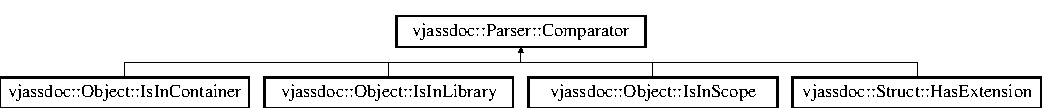
\includegraphics[height=1.45078cm]{structvjassdoc_1_1Parser_1_1Comparator}
\end{center}
\end{figure}
\subsection*{Public Member Functions}
\begin{CompactItemize}
\item 
virtual bool \hyperlink{structvjassdoc_1_1Parser_1_1Comparator_c27d6790182d87751bcf134a0d01481a}{operator()} (const class \hyperlink{classvjassdoc_1_1Object}{Object} $\ast$thisObject, const class \hyperlink{classvjassdoc_1_1Object}{Object} $\ast$otherObject) const 
\end{CompactItemize}


\subsection{Member Function Documentation}
\hypertarget{structvjassdoc_1_1Parser_1_1Comparator_c27d6790182d87751bcf134a0d01481a}{
\index{vjassdoc::Parser::Comparator@{vjassdoc::Parser::Comparator}!operator()@{operator()}}
\index{operator()@{operator()}!vjassdoc::Parser::Comparator@{vjassdoc::Parser::Comparator}}
\subsubsection{\setlength{\rightskip}{0pt plus 5cm}bool vjassdoc::Parser::Comparator::operator() (const class {\bf Object} $\ast$ {\em thisObject}, const class {\bf Object} $\ast$ {\em otherObject}) const\hspace{0.3cm}{\tt  \mbox{[}virtual\mbox{]}}}}
\label{structvjassdoc_1_1Parser_1_1Comparator_c27d6790182d87751bcf134a0d01481a}




Reimplemented in \hyperlink{structvjassdoc_1_1Object_1_1IsInContainer_390275d3950a824ad1a9ac025964ef64}{vjassdoc::Object::IsInContainer}, \hyperlink{structvjassdoc_1_1Object_1_1IsInScope_319d4736b3b35681570cc5be477dc5c9}{vjassdoc::Object::IsInScope}, \hyperlink{structvjassdoc_1_1Object_1_1IsInLibrary_a1a041f942f665e8f62e30fa2ad3b260}{vjassdoc::Object::IsInLibrary}, and \hyperlink{structvjassdoc_1_1Struct_1_1HasExtension_9e08804f805e2ba8616088ec0bfe84e2}{vjassdoc::Struct::HasExtension}.

The documentation for this struct was generated from the following files:\begin{CompactItemize}
\item 
src/\hyperlink{parser_8h}{parser.h}\item 
src/\hyperlink{parser_8cpp}{parser.cpp}\end{CompactItemize}

\hypertarget{classvjassdoc_1_1Scope}{
\section{vjassdoc::Scope Class Reference}
\label{classvjassdoc_1_1Scope}\index{vjassdoc::Scope@{vjassdoc::Scope}}
}
{\tt \#include $<$scope.h$>$}

Inheritance diagram for vjassdoc::Scope::\begin{figure}[H]
\begin{center}
\leavevmode
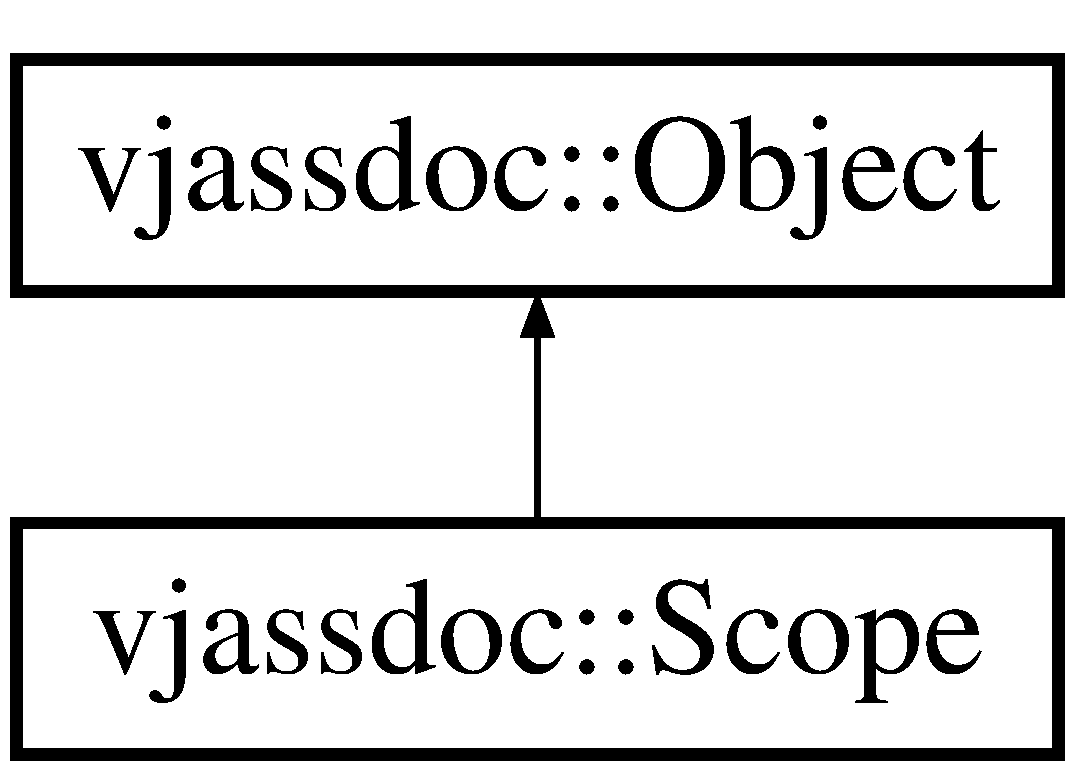
\includegraphics[height=2cm]{classvjassdoc_1_1Scope}
\end{center}
\end{figure}
\subsection*{Public Member Functions}
\begin{CompactItemize}
\item 
\hyperlink{classvjassdoc_1_1Scope_93e1a8c864401dcb118123b8c1c862d8}{Scope} (const std::string \&identifier, class \hyperlink{classvjassdoc_1_1SourceFile}{SourceFile} $\ast$sourceFile, unsigned int line, class \hyperlink{classvjassdoc_1_1DocComment}{DocComment} $\ast$docComment, class \hyperlink{classvjassdoc_1_1Library}{Library} $\ast$library, bool isPrivate, const std::string initializerExpression)
\item 
\hyperlink{classvjassdoc_1_1Scope_08fa49b1daca27363032265465005dc0}{Scope} (std::vector$<$ const unsigned char $\ast$ $>$ \&columnVector)
\item 
virtual void \hyperlink{classvjassdoc_1_1Scope_fb5915ecd0cabc72508e7b7a09f0ef5c}{init} ()
\item 
virtual void \hyperlink{classvjassdoc_1_1Scope_3fac1b4e0201e20463acfc5f0f0e93b8}{pageNavigation} (std::ofstream \&file) const 
\item 
virtual void \hyperlink{classvjassdoc_1_1Scope_2a37c9d88da6a8c7c95d4f0e5b88ccbb}{page} (std::ofstream \&file) const 
\item 
virtual std::string \hyperlink{classvjassdoc_1_1Scope_634ae4bc06389b21ef8612795d4a910f}{sqlStatement} () const 
\item 
virtual class \hyperlink{classvjassdoc_1_1Library}{Library} $\ast$ \hyperlink{classvjassdoc_1_1Scope_4d9d486897a1960cff057ab88a43fb15}{library} () const 
\item 
bool \hyperlink{classvjassdoc_1_1Scope_c2b7a4d2f0a0e248194d9e96c3d00f10}{isPrivate} () const 
\item 
class \hyperlink{classvjassdoc_1_1Function}{Function} $\ast$ \hyperlink{classvjassdoc_1_1Scope_33866d7c3eac290c01e57e1919b26cda}{initializer} () const 
\end{CompactItemize}


\subsection{Constructor \& Destructor Documentation}
\hypertarget{classvjassdoc_1_1Scope_93e1a8c864401dcb118123b8c1c862d8}{
\index{vjassdoc::Scope@{vjassdoc::Scope}!Scope@{Scope}}
\index{Scope@{Scope}!vjassdoc::Scope@{vjassdoc::Scope}}
\subsubsection{\setlength{\rightskip}{0pt plus 5cm}vjassdoc::Scope::Scope (const std::string \& {\em identifier}, class {\bf SourceFile} $\ast$ {\em sourceFile}, unsigned int {\em line}, class {\bf DocComment} $\ast$ {\em docComment}, class {\bf Library} $\ast$ {\em library}, bool {\em isPrivate}, const std::string {\em initializerExpression})}}
\label{classvjassdoc_1_1Scope_93e1a8c864401dcb118123b8c1c862d8}


\hypertarget{classvjassdoc_1_1Scope_08fa49b1daca27363032265465005dc0}{
\index{vjassdoc::Scope@{vjassdoc::Scope}!Scope@{Scope}}
\index{Scope@{Scope}!vjassdoc::Scope@{vjassdoc::Scope}}
\subsubsection{\setlength{\rightskip}{0pt plus 5cm}vjassdoc::Scope::Scope (std::vector$<$ const unsigned char $\ast$ $>$ \& {\em columnVector})}}
\label{classvjassdoc_1_1Scope_08fa49b1daca27363032265465005dc0}




\subsection{Member Function Documentation}
\hypertarget{classvjassdoc_1_1Scope_fb5915ecd0cabc72508e7b7a09f0ef5c}{
\index{vjassdoc::Scope@{vjassdoc::Scope}!init@{init}}
\index{init@{init}!vjassdoc::Scope@{vjassdoc::Scope}}
\subsubsection{\setlength{\rightskip}{0pt plus 5cm}void vjassdoc::Scope::init ()\hspace{0.3cm}{\tt  \mbox{[}virtual\mbox{]}}}}
\label{classvjassdoc_1_1Scope_fb5915ecd0cabc72508e7b7a09f0ef5c}




Implements \hyperlink{classvjassdoc_1_1Object_bd43e77dbe80055f5adda67661dfaca4}{vjassdoc::Object}.\hypertarget{classvjassdoc_1_1Scope_3fac1b4e0201e20463acfc5f0f0e93b8}{
\index{vjassdoc::Scope@{vjassdoc::Scope}!pageNavigation@{pageNavigation}}
\index{pageNavigation@{pageNavigation}!vjassdoc::Scope@{vjassdoc::Scope}}
\subsubsection{\setlength{\rightskip}{0pt plus 5cm}void vjassdoc::Scope::pageNavigation (std::ofstream \& {\em file}) const\hspace{0.3cm}{\tt  \mbox{[}virtual\mbox{]}}}}
\label{classvjassdoc_1_1Scope_3fac1b4e0201e20463acfc5f0f0e93b8}




Implements \hyperlink{classvjassdoc_1_1Object_736bbb6719edd8070d8f56c364a2764c}{vjassdoc::Object}.\hypertarget{classvjassdoc_1_1Scope_2a37c9d88da6a8c7c95d4f0e5b88ccbb}{
\index{vjassdoc::Scope@{vjassdoc::Scope}!page@{page}}
\index{page@{page}!vjassdoc::Scope@{vjassdoc::Scope}}
\subsubsection{\setlength{\rightskip}{0pt plus 5cm}void vjassdoc::Scope::page (std::ofstream \& {\em file}) const\hspace{0.3cm}{\tt  \mbox{[}virtual\mbox{]}}}}
\label{classvjassdoc_1_1Scope_2a37c9d88da6a8c7c95d4f0e5b88ccbb}




Implements \hyperlink{classvjassdoc_1_1Object_a0489e38956f3507566b1bc6e3e2c8af}{vjassdoc::Object}.\hypertarget{classvjassdoc_1_1Scope_634ae4bc06389b21ef8612795d4a910f}{
\index{vjassdoc::Scope@{vjassdoc::Scope}!sqlStatement@{sqlStatement}}
\index{sqlStatement@{sqlStatement}!vjassdoc::Scope@{vjassdoc::Scope}}
\subsubsection{\setlength{\rightskip}{0pt plus 5cm}std::string vjassdoc::Scope::sqlStatement () const\hspace{0.3cm}{\tt  \mbox{[}virtual\mbox{]}}}}
\label{classvjassdoc_1_1Scope_634ae4bc06389b21ef8612795d4a910f}




Reimplemented from \hyperlink{classvjassdoc_1_1Object_4e8ebbb0ce5b0bf91ec847b1e4a9f8fc}{vjassdoc::Object}.\hypertarget{classvjassdoc_1_1Scope_4d9d486897a1960cff057ab88a43fb15}{
\index{vjassdoc::Scope@{vjassdoc::Scope}!library@{library}}
\index{library@{library}!vjassdoc::Scope@{vjassdoc::Scope}}
\subsubsection{\setlength{\rightskip}{0pt plus 5cm}class {\bf Library} $\ast$ vjassdoc::Scope::library () const\hspace{0.3cm}{\tt  \mbox{[}virtual\mbox{]}}}}
\label{classvjassdoc_1_1Scope_4d9d486897a1960cff057ab88a43fb15}




Reimplemented from \hyperlink{classvjassdoc_1_1Object_cc4241505c5bcdd0bbcb08a1b665b3fd}{vjassdoc::Object}.\hypertarget{classvjassdoc_1_1Scope_c2b7a4d2f0a0e248194d9e96c3d00f10}{
\index{vjassdoc::Scope@{vjassdoc::Scope}!isPrivate@{isPrivate}}
\index{isPrivate@{isPrivate}!vjassdoc::Scope@{vjassdoc::Scope}}
\subsubsection{\setlength{\rightskip}{0pt plus 5cm}bool vjassdoc::Scope::isPrivate () const\hspace{0.3cm}{\tt  \mbox{[}inline\mbox{]}}}}
\label{classvjassdoc_1_1Scope_c2b7a4d2f0a0e248194d9e96c3d00f10}


\hypertarget{classvjassdoc_1_1Scope_33866d7c3eac290c01e57e1919b26cda}{
\index{vjassdoc::Scope@{vjassdoc::Scope}!initializer@{initializer}}
\index{initializer@{initializer}!vjassdoc::Scope@{vjassdoc::Scope}}
\subsubsection{\setlength{\rightskip}{0pt plus 5cm}class {\bf Function} $\ast$ vjassdoc::Scope::initializer () const\hspace{0.3cm}{\tt  \mbox{[}inline\mbox{]}}}}
\label{classvjassdoc_1_1Scope_33866d7c3eac290c01e57e1919b26cda}




The documentation for this class was generated from the following files:\begin{CompactItemize}
\item 
src/\hyperlink{scope_8h}{scope.h}\item 
src/\hyperlink{scope_8cpp}{scope.cpp}\end{CompactItemize}

\hypertarget{classvjassdoc_1_1SourceFile}{
\section{vjassdoc::SourceFile Class Reference}
\label{classvjassdoc_1_1SourceFile}\index{vjassdoc::SourceFile@{vjassdoc::SourceFile}}
}
{\tt \#include $<$sourcefile.h$>$}

Inheritance diagram for vjassdoc::SourceFile::\begin{figure}[H]
\begin{center}
\leavevmode
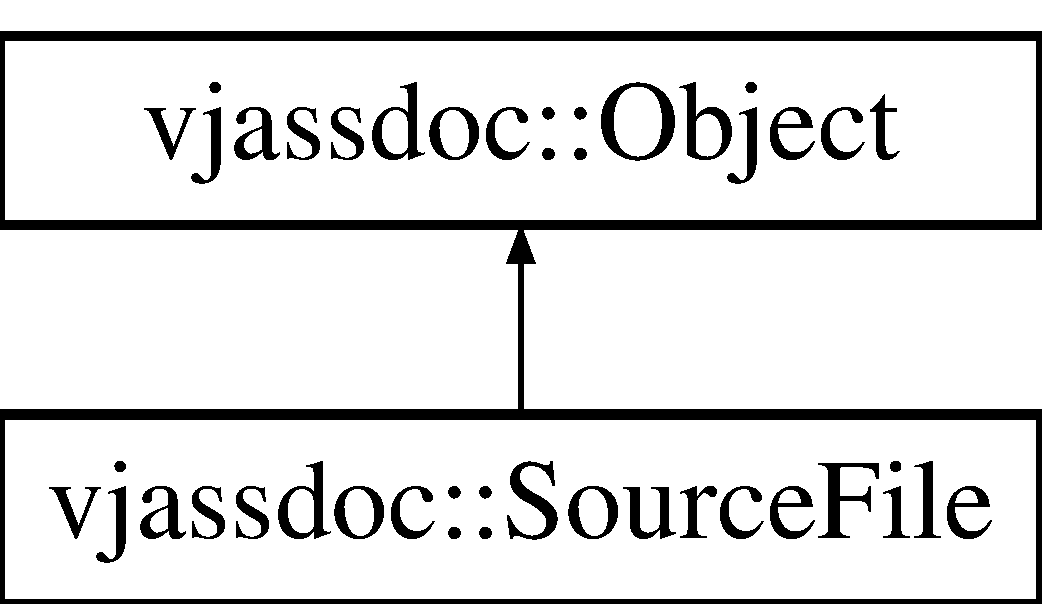
\includegraphics[height=2cm]{classvjassdoc_1_1SourceFile}
\end{center}
\end{figure}
\subsection*{Public Member Functions}
\begin{CompactItemize}
\item 
\hyperlink{classvjassdoc_1_1SourceFile_e4dd92032b7498bf71ddb71daa30253a}{SourceFile} (const std::string \&identifier, const std::string \&path)
\item 
\hyperlink{classvjassdoc_1_1SourceFile_e0d55673a13f69697ed0dd2130b9535b}{SourceFile} (std::vector$<$ const unsigned char $\ast$ $>$ \&columnVector)
\item 
virtual void \hyperlink{classvjassdoc_1_1SourceFile_e2aa3f034bbb18de023ce9a21dfa78d1}{init} ()
\item 
virtual void \hyperlink{classvjassdoc_1_1SourceFile_b365551c64c03553e8fb1a31d83edaea}{pageNavigation} (std::ofstream \&file) const 
\item 
virtual void \hyperlink{classvjassdoc_1_1SourceFile_0a4aed2c620f52f3cb114843f674b31c}{page} (std::ofstream \&file) const 
\item 
virtual std::string \hyperlink{classvjassdoc_1_1SourceFile_cda6410687f71928eafac94a635c4250}{sqlStatement} () const 
\item 
std::string \hyperlink{classvjassdoc_1_1SourceFile_4764039ae2d00f6fbdc41186972b5ff9}{path} () const 
\item 
std::string \hyperlink{classvjassdoc_1_1SourceFile_b470fdc8f3bb45197ba3ca3fd7aefbea}{lineLink} (const unsigned int \&line, const std::string \&text) const 
\end{CompactItemize}
\subsection*{Static Public Member Functions}
\begin{CompactItemize}
\item 
static std::string \hyperlink{classvjassdoc_1_1SourceFile_5442b71bdf46f52e3aec90257e6a3dcb}{sourceFileLineLink} (const class \hyperlink{classvjassdoc_1_1Object}{Object} $\ast$object, const bool \&sourceFileName=true, const std::string \&identifier=\char`\"{}-\char`\"{})
\end{CompactItemize}


\subsection{Constructor \& Destructor Documentation}
\hypertarget{classvjassdoc_1_1SourceFile_e4dd92032b7498bf71ddb71daa30253a}{
\index{vjassdoc::SourceFile@{vjassdoc::SourceFile}!SourceFile@{SourceFile}}
\index{SourceFile@{SourceFile}!vjassdoc::SourceFile@{vjassdoc::SourceFile}}
\subsubsection{\setlength{\rightskip}{0pt plus 5cm}vjassdoc::SourceFile::SourceFile (const std::string \& {\em identifier}, const std::string \& {\em path})}}
\label{classvjassdoc_1_1SourceFile_e4dd92032b7498bf71ddb71daa30253a}


\hypertarget{classvjassdoc_1_1SourceFile_e0d55673a13f69697ed0dd2130b9535b}{
\index{vjassdoc::SourceFile@{vjassdoc::SourceFile}!SourceFile@{SourceFile}}
\index{SourceFile@{SourceFile}!vjassdoc::SourceFile@{vjassdoc::SourceFile}}
\subsubsection{\setlength{\rightskip}{0pt plus 5cm}vjassdoc::SourceFile::SourceFile (std::vector$<$ const unsigned char $\ast$ $>$ \& {\em columnVector})}}
\label{classvjassdoc_1_1SourceFile_e0d55673a13f69697ed0dd2130b9535b}




\subsection{Member Function Documentation}
\hypertarget{classvjassdoc_1_1SourceFile_e2aa3f034bbb18de023ce9a21dfa78d1}{
\index{vjassdoc::SourceFile@{vjassdoc::SourceFile}!init@{init}}
\index{init@{init}!vjassdoc::SourceFile@{vjassdoc::SourceFile}}
\subsubsection{\setlength{\rightskip}{0pt plus 5cm}void vjassdoc::SourceFile::init ()\hspace{0.3cm}{\tt  \mbox{[}virtual\mbox{]}}}}
\label{classvjassdoc_1_1SourceFile_e2aa3f034bbb18de023ce9a21dfa78d1}




Implements \hyperlink{classvjassdoc_1_1Object_bd43e77dbe80055f5adda67661dfaca4}{vjassdoc::Object}.\hypertarget{classvjassdoc_1_1SourceFile_b365551c64c03553e8fb1a31d83edaea}{
\index{vjassdoc::SourceFile@{vjassdoc::SourceFile}!pageNavigation@{pageNavigation}}
\index{pageNavigation@{pageNavigation}!vjassdoc::SourceFile@{vjassdoc::SourceFile}}
\subsubsection{\setlength{\rightskip}{0pt plus 5cm}void vjassdoc::SourceFile::pageNavigation (std::ofstream \& {\em file}) const\hspace{0.3cm}{\tt  \mbox{[}virtual\mbox{]}}}}
\label{classvjassdoc_1_1SourceFile_b365551c64c03553e8fb1a31d83edaea}




Implements \hyperlink{classvjassdoc_1_1Object_736bbb6719edd8070d8f56c364a2764c}{vjassdoc::Object}.\hypertarget{classvjassdoc_1_1SourceFile_0a4aed2c620f52f3cb114843f674b31c}{
\index{vjassdoc::SourceFile@{vjassdoc::SourceFile}!page@{page}}
\index{page@{page}!vjassdoc::SourceFile@{vjassdoc::SourceFile}}
\subsubsection{\setlength{\rightskip}{0pt plus 5cm}void vjassdoc::SourceFile::page (std::ofstream \& {\em file}) const\hspace{0.3cm}{\tt  \mbox{[}virtual\mbox{]}}}}
\label{classvjassdoc_1_1SourceFile_0a4aed2c620f52f3cb114843f674b31c}




Implements \hyperlink{classvjassdoc_1_1Object_a0489e38956f3507566b1bc6e3e2c8af}{vjassdoc::Object}.\hypertarget{classvjassdoc_1_1SourceFile_cda6410687f71928eafac94a635c4250}{
\index{vjassdoc::SourceFile@{vjassdoc::SourceFile}!sqlStatement@{sqlStatement}}
\index{sqlStatement@{sqlStatement}!vjassdoc::SourceFile@{vjassdoc::SourceFile}}
\subsubsection{\setlength{\rightskip}{0pt plus 5cm}std::string vjassdoc::SourceFile::sqlStatement () const\hspace{0.3cm}{\tt  \mbox{[}virtual\mbox{]}}}}
\label{classvjassdoc_1_1SourceFile_cda6410687f71928eafac94a635c4250}




Reimplemented from \hyperlink{classvjassdoc_1_1Object_4e8ebbb0ce5b0bf91ec847b1e4a9f8fc}{vjassdoc::Object}.\hypertarget{classvjassdoc_1_1SourceFile_4764039ae2d00f6fbdc41186972b5ff9}{
\index{vjassdoc::SourceFile@{vjassdoc::SourceFile}!path@{path}}
\index{path@{path}!vjassdoc::SourceFile@{vjassdoc::SourceFile}}
\subsubsection{\setlength{\rightskip}{0pt plus 5cm}std::string vjassdoc::SourceFile::path () const\hspace{0.3cm}{\tt  \mbox{[}inline\mbox{]}}}}
\label{classvjassdoc_1_1SourceFile_4764039ae2d00f6fbdc41186972b5ff9}


\hypertarget{classvjassdoc_1_1SourceFile_b470fdc8f3bb45197ba3ca3fd7aefbea}{
\index{vjassdoc::SourceFile@{vjassdoc::SourceFile}!lineLink@{lineLink}}
\index{lineLink@{lineLink}!vjassdoc::SourceFile@{vjassdoc::SourceFile}}
\subsubsection{\setlength{\rightskip}{0pt plus 5cm}std::string vjassdoc::SourceFile::lineLink (const unsigned int \& {\em line}, const std::string \& {\em text}) const\hspace{0.3cm}{\tt  \mbox{[}inline\mbox{]}}}}
\label{classvjassdoc_1_1SourceFile_b470fdc8f3bb45197ba3ca3fd7aefbea}


\hypertarget{classvjassdoc_1_1SourceFile_5442b71bdf46f52e3aec90257e6a3dcb}{
\index{vjassdoc::SourceFile@{vjassdoc::SourceFile}!sourceFileLineLink@{sourceFileLineLink}}
\index{sourceFileLineLink@{sourceFileLineLink}!vjassdoc::SourceFile@{vjassdoc::SourceFile}}
\subsubsection{\setlength{\rightskip}{0pt plus 5cm}std::string vjassdoc::SourceFile::sourceFileLineLink (const class {\bf Object} $\ast$ {\em object}, const bool \& {\em sourceFileName} = {\tt true}, const std::string \& {\em identifier} = {\tt \char`\"{}-\char`\"{}})\hspace{0.3cm}{\tt  \mbox{[}inline, static\mbox{]}}}}
\label{classvjassdoc_1_1SourceFile_5442b71bdf46f52e3aec90257e6a3dcb}


\begin{Desc}
\item[Parameters:]
\begin{description}
\item[{\em sourceFileName}]If this value is true, the name of source file will be shown as link. Otherwise the line will be shown. \end{description}
\end{Desc}


The documentation for this class was generated from the following files:\begin{CompactItemize}
\item 
src/\hyperlink{sourcefile_8h}{sourcefile.h}\item 
src/\hyperlink{sourcefile_8cpp}{sourcefile.cpp}\end{CompactItemize}

\hypertarget{classvjassdoc_1_1Struct}{
\section{vjassdoc::Struct Class Reference}
\label{classvjassdoc_1_1Struct}\index{vjassdoc::Struct@{vjassdoc::Struct}}
}
{\tt \#include $<$struct.h$>$}

Inheritance diagram for vjassdoc::Struct::\begin{figure}[H]
\begin{center}
\leavevmode
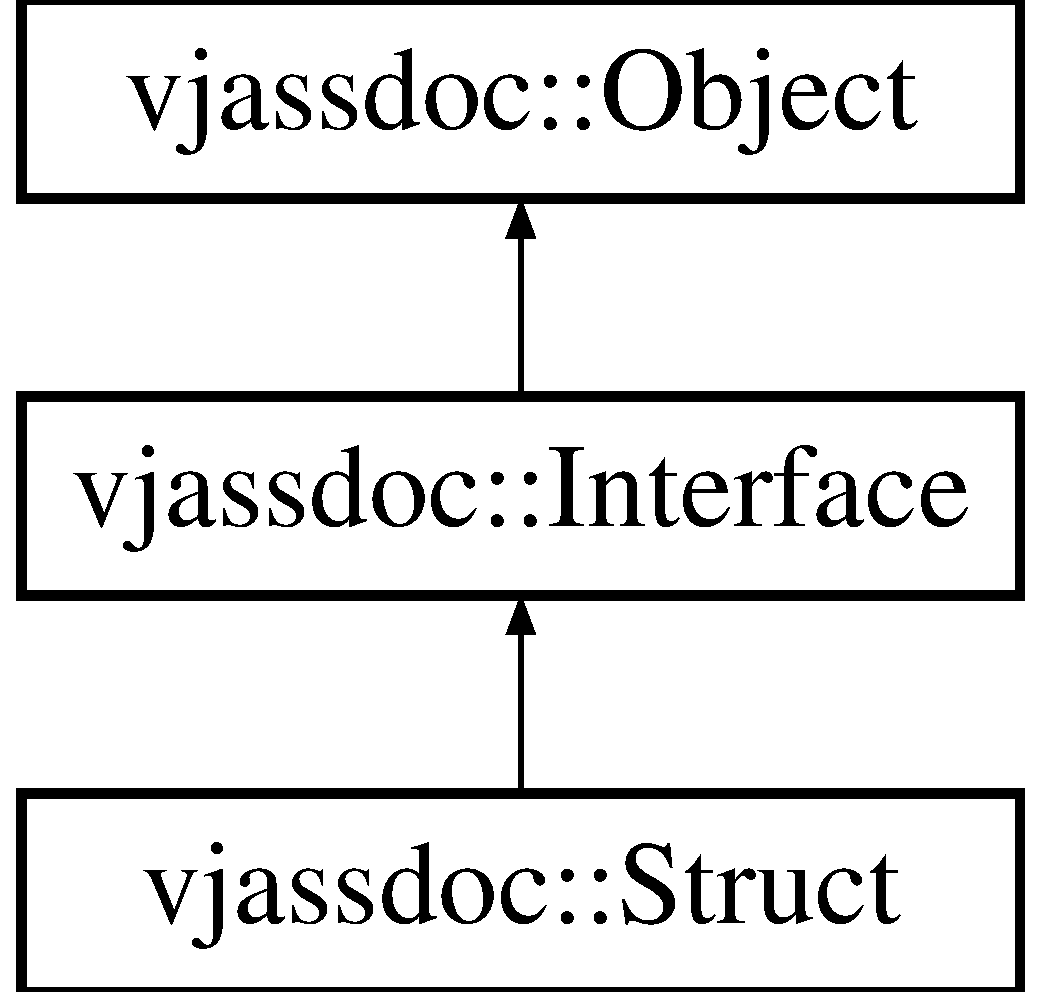
\includegraphics[height=3cm]{classvjassdoc_1_1Struct}
\end{center}
\end{figure}
\subsection*{Public Member Functions}
\begin{CompactItemize}
\item 
\hyperlink{classvjassdoc_1_1Struct_3c985875cff8b6b41f1193aa0bdd124f}{Struct} (const std::string \&identifier, class \hyperlink{classvjassdoc_1_1SourceFile}{SourceFile} $\ast$sourceFile, unsigned int line, class \hyperlink{classvjassdoc_1_1DocComment}{DocComment} $\ast$docComment, class \hyperlink{classvjassdoc_1_1Library}{Library} $\ast$library, \hyperlink{classvjassdoc_1_1Scope}{Scope} $\ast$scope, bool isPrivate, const std::string \&extensionExpression)
\item 
\hyperlink{classvjassdoc_1_1Struct_577a9bb757bf7775389eb8e6e59dee1a}{Struct} (std::vector$<$ const unsigned char $\ast$ $>$ \&columnVector)
\item 
virtual void \hyperlink{classvjassdoc_1_1Struct_39dc86da31e526f3a6eb3b6e442156bb}{init} ()
\item 
virtual void \hyperlink{classvjassdoc_1_1Struct_c415c5b26f7385a990339dfbfbbca5dc}{pageNavigation} (std::ofstream \&file) const 
\item 
virtual void \hyperlink{classvjassdoc_1_1Struct_bd918c5a1ec7defe1849f4b4e61523f2}{page} (std::ofstream \&file) const 
\item 
virtual std::string \hyperlink{classvjassdoc_1_1Struct_227d826acdbbe1702941634c90ab7e4e}{sqlStatement} () const 
\item 
class \hyperlink{classvjassdoc_1_1Interface}{Interface} $\ast$ \hyperlink{classvjassdoc_1_1Struct_92ef4086c680565cd9c5766607d8a560}{extension} () const 
\item 
class \hyperlink{classvjassdoc_1_1Method}{Method} $\ast$ \hyperlink{classvjassdoc_1_1Struct_41a8c77e86a5a04ee3e594c58e0f4ceb}{constructor} () const 
\item 
class \hyperlink{classvjassdoc_1_1Method}{Method} $\ast$ \hyperlink{classvjassdoc_1_1Struct_f4c2781402019fade0e674abbd5f161b}{destructor} () const 
\item 
class \hyperlink{classvjassdoc_1_1Method}{Method} $\ast$ \hyperlink{classvjassdoc_1_1Struct_234bd98d0902f34047f17f005a5f1dbe}{initializer} () const 
\end{CompactItemize}
\subsection*{Classes}
\begin{CompactItemize}
\item 
struct \hyperlink{structvjassdoc_1_1Struct_1_1HasExtension}{HasExtension}
\end{CompactItemize}


\subsection{Constructor \& Destructor Documentation}
\hypertarget{classvjassdoc_1_1Struct_3c985875cff8b6b41f1193aa0bdd124f}{
\index{vjassdoc::Struct@{vjassdoc::Struct}!Struct@{Struct}}
\index{Struct@{Struct}!vjassdoc::Struct@{vjassdoc::Struct}}
\subsubsection{\setlength{\rightskip}{0pt plus 5cm}vjassdoc::Struct::Struct (const std::string \& {\em identifier}, class {\bf SourceFile} $\ast$ {\em sourceFile}, unsigned int {\em line}, class {\bf DocComment} $\ast$ {\em docComment}, class {\bf Library} $\ast$ {\em library}, {\bf Scope} $\ast$ {\em scope}, bool {\em isPrivate}, const std::string \& {\em extensionExpression})}}
\label{classvjassdoc_1_1Struct_3c985875cff8b6b41f1193aa0bdd124f}


\hypertarget{classvjassdoc_1_1Struct_577a9bb757bf7775389eb8e6e59dee1a}{
\index{vjassdoc::Struct@{vjassdoc::Struct}!Struct@{Struct}}
\index{Struct@{Struct}!vjassdoc::Struct@{vjassdoc::Struct}}
\subsubsection{\setlength{\rightskip}{0pt plus 5cm}vjassdoc::Struct::Struct (std::vector$<$ const unsigned char $\ast$ $>$ \& {\em columnVector})}}
\label{classvjassdoc_1_1Struct_577a9bb757bf7775389eb8e6e59dee1a}




\subsection{Member Function Documentation}
\hypertarget{classvjassdoc_1_1Struct_39dc86da31e526f3a6eb3b6e442156bb}{
\index{vjassdoc::Struct@{vjassdoc::Struct}!init@{init}}
\index{init@{init}!vjassdoc::Struct@{vjassdoc::Struct}}
\subsubsection{\setlength{\rightskip}{0pt plus 5cm}void vjassdoc::Struct::init ()\hspace{0.3cm}{\tt  \mbox{[}virtual\mbox{]}}}}
\label{classvjassdoc_1_1Struct_39dc86da31e526f3a6eb3b6e442156bb}




Reimplemented from \hyperlink{classvjassdoc_1_1Interface_e10d2a4a6acf44897145bf76675b9da1}{vjassdoc::Interface}.\hypertarget{classvjassdoc_1_1Struct_c415c5b26f7385a990339dfbfbbca5dc}{
\index{vjassdoc::Struct@{vjassdoc::Struct}!pageNavigation@{pageNavigation}}
\index{pageNavigation@{pageNavigation}!vjassdoc::Struct@{vjassdoc::Struct}}
\subsubsection{\setlength{\rightskip}{0pt plus 5cm}void vjassdoc::Struct::pageNavigation (std::ofstream \& {\em file}) const\hspace{0.3cm}{\tt  \mbox{[}virtual\mbox{]}}}}
\label{classvjassdoc_1_1Struct_c415c5b26f7385a990339dfbfbbca5dc}




Reimplemented from \hyperlink{classvjassdoc_1_1Interface_f0acc07a23eb46eb9f065fb47d55f1a5}{vjassdoc::Interface}.\hypertarget{classvjassdoc_1_1Struct_bd918c5a1ec7defe1849f4b4e61523f2}{
\index{vjassdoc::Struct@{vjassdoc::Struct}!page@{page}}
\index{page@{page}!vjassdoc::Struct@{vjassdoc::Struct}}
\subsubsection{\setlength{\rightskip}{0pt plus 5cm}void vjassdoc::Struct::page (std::ofstream \& {\em file}) const\hspace{0.3cm}{\tt  \mbox{[}virtual\mbox{]}}}}
\label{classvjassdoc_1_1Struct_bd918c5a1ec7defe1849f4b4e61523f2}




Reimplemented from \hyperlink{classvjassdoc_1_1Interface_79ed4ee7fd055e3b53fdb9b14749fa0f}{vjassdoc::Interface}.\hypertarget{classvjassdoc_1_1Struct_227d826acdbbe1702941634c90ab7e4e}{
\index{vjassdoc::Struct@{vjassdoc::Struct}!sqlStatement@{sqlStatement}}
\index{sqlStatement@{sqlStatement}!vjassdoc::Struct@{vjassdoc::Struct}}
\subsubsection{\setlength{\rightskip}{0pt plus 5cm}std::string vjassdoc::Struct::sqlStatement () const\hspace{0.3cm}{\tt  \mbox{[}virtual\mbox{]}}}}
\label{classvjassdoc_1_1Struct_227d826acdbbe1702941634c90ab7e4e}




Reimplemented from \hyperlink{classvjassdoc_1_1Interface_93fbe7323df0502111e576c08376b726}{vjassdoc::Interface}.\hypertarget{classvjassdoc_1_1Struct_92ef4086c680565cd9c5766607d8a560}{
\index{vjassdoc::Struct@{vjassdoc::Struct}!extension@{extension}}
\index{extension@{extension}!vjassdoc::Struct@{vjassdoc::Struct}}
\subsubsection{\setlength{\rightskip}{0pt plus 5cm}class {\bf Interface} $\ast$ vjassdoc::Struct::extension () const\hspace{0.3cm}{\tt  \mbox{[}inline\mbox{]}}}}
\label{classvjassdoc_1_1Struct_92ef4086c680565cd9c5766607d8a560}


\hypertarget{classvjassdoc_1_1Struct_41a8c77e86a5a04ee3e594c58e0f4ceb}{
\index{vjassdoc::Struct@{vjassdoc::Struct}!constructor@{constructor}}
\index{constructor@{constructor}!vjassdoc::Struct@{vjassdoc::Struct}}
\subsubsection{\setlength{\rightskip}{0pt plus 5cm}class {\bf Method} $\ast$ vjassdoc::Struct::constructor () const\hspace{0.3cm}{\tt  \mbox{[}inline\mbox{]}}}}
\label{classvjassdoc_1_1Struct_41a8c77e86a5a04ee3e594c58e0f4ceb}


\hypertarget{classvjassdoc_1_1Struct_f4c2781402019fade0e674abbd5f161b}{
\index{vjassdoc::Struct@{vjassdoc::Struct}!destructor@{destructor}}
\index{destructor@{destructor}!vjassdoc::Struct@{vjassdoc::Struct}}
\subsubsection{\setlength{\rightskip}{0pt plus 5cm}class {\bf Method} $\ast$ vjassdoc::Struct::destructor () const\hspace{0.3cm}{\tt  \mbox{[}inline\mbox{]}}}}
\label{classvjassdoc_1_1Struct_f4c2781402019fade0e674abbd5f161b}


\hypertarget{classvjassdoc_1_1Struct_234bd98d0902f34047f17f005a5f1dbe}{
\index{vjassdoc::Struct@{vjassdoc::Struct}!initializer@{initializer}}
\index{initializer@{initializer}!vjassdoc::Struct@{vjassdoc::Struct}}
\subsubsection{\setlength{\rightskip}{0pt plus 5cm}class {\bf Method} $\ast$ vjassdoc::Struct::initializer () const\hspace{0.3cm}{\tt  \mbox{[}inline\mbox{]}}}}
\label{classvjassdoc_1_1Struct_234bd98d0902f34047f17f005a5f1dbe}




The documentation for this class was generated from the following files:\begin{CompactItemize}
\item 
src/\hyperlink{struct_8h}{struct.h}\item 
src/\hyperlink{struct_8cpp}{struct.cpp}\end{CompactItemize}

\hypertarget{structvjassdoc_1_1Struct_1_1HasExtension}{
\section{vjassdoc::Struct::HasExtension Struct Reference}
\label{structvjassdoc_1_1Struct_1_1HasExtension}\index{vjassdoc::Struct::HasExtension@{vjassdoc::Struct::HasExtension}}
}
{\tt \#include $<$struct.h$>$}

Inheritance diagram for vjassdoc::Struct::HasExtension::\begin{figure}[H]
\begin{center}
\leavevmode
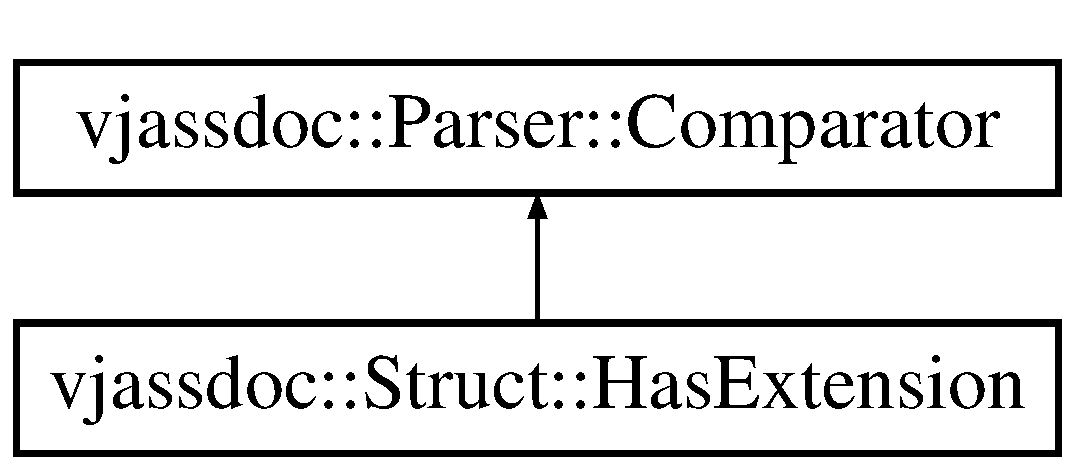
\includegraphics[height=2cm]{structvjassdoc_1_1Struct_1_1HasExtension}
\end{center}
\end{figure}
\subsection*{Public Member Functions}
\begin{CompactItemize}
\item 
virtual bool \hyperlink{structvjassdoc_1_1Struct_1_1HasExtension_9e08804f805e2ba8616088ec0bfe84e2}{operator()} (const class \hyperlink{classvjassdoc_1_1Object}{Object} $\ast$thisObject, const class \hyperlink{classvjassdoc_1_1Object}{Object} $\ast$extension) const 
\end{CompactItemize}


\subsection{Member Function Documentation}
\hypertarget{structvjassdoc_1_1Struct_1_1HasExtension_9e08804f805e2ba8616088ec0bfe84e2}{
\index{vjassdoc::Struct::HasExtension@{vjassdoc::Struct::HasExtension}!operator()@{operator()}}
\index{operator()@{operator()}!vjassdoc::Struct::HasExtension@{vjassdoc::Struct::HasExtension}}
\subsubsection{\setlength{\rightskip}{0pt plus 5cm}bool vjassdoc::Struct::HasExtension::operator() (const class {\bf Object} $\ast$ {\em thisObject}, const class {\bf Object} $\ast$ {\em extension}) const\hspace{0.3cm}{\tt  \mbox{[}virtual\mbox{]}}}}
\label{structvjassdoc_1_1Struct_1_1HasExtension_9e08804f805e2ba8616088ec0bfe84e2}




Reimplemented from \hyperlink{structvjassdoc_1_1Parser_1_1Comparator_c27d6790182d87751bcf134a0d01481a}{vjassdoc::Parser::Comparator}.

The documentation for this struct was generated from the following files:\begin{CompactItemize}
\item 
src/\hyperlink{struct_8h}{struct.h}\item 
src/\hyperlink{struct_8cpp}{struct.cpp}\end{CompactItemize}

\hypertarget{classvjassdoc_1_1TextMacro}{
\section{vjassdoc::TextMacro Class Reference}
\label{classvjassdoc_1_1TextMacro}\index{vjassdoc::TextMacro@{vjassdoc::TextMacro}}
}
{\tt \#include $<$textmacro.h$>$}

Inheritance diagram for vjassdoc::TextMacro::\begin{figure}[H]
\begin{center}
\leavevmode
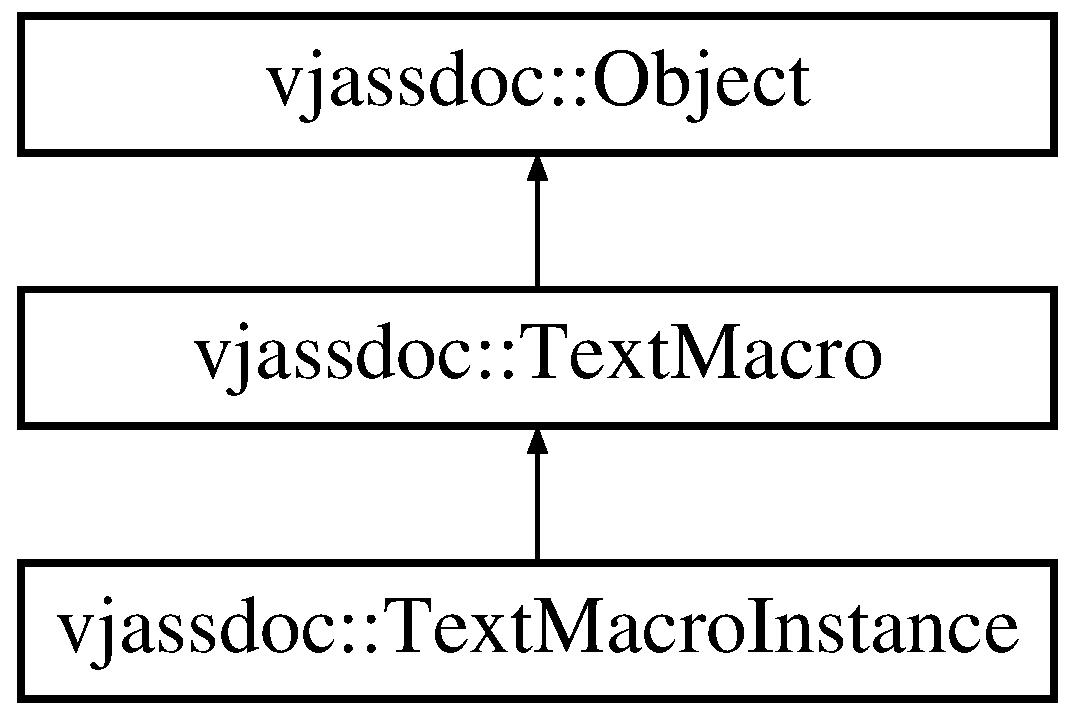
\includegraphics[height=3cm]{classvjassdoc_1_1TextMacro}
\end{center}
\end{figure}
\subsection*{Public Member Functions}
\begin{CompactItemize}
\item 
\hyperlink{classvjassdoc_1_1TextMacro_7354fb20a513ca489afe554896f039ef}{TextMacro} (const std::string \&identifier, class \hyperlink{classvjassdoc_1_1SourceFile}{SourceFile} $\ast$sourceFile, unsigned int line, class \hyperlink{classvjassdoc_1_1DocComment}{DocComment} $\ast$docComment, const std::string \&parameters)
\item 
\hyperlink{classvjassdoc_1_1TextMacro_c82712ca934e5a59bff730add064ec78}{TextMacro} (std::vector$<$ const unsigned char $\ast$ $>$ \&columnVector)
\item 
virtual void \hyperlink{classvjassdoc_1_1TextMacro_816bdd2b838a4f1148ea17e5723e8577}{init} ()
\item 
virtual void \hyperlink{classvjassdoc_1_1TextMacro_d3ad5fe5300492db3d1aaf250d9b2a4b}{pageNavigation} (std::ofstream \&file) const 
\item 
virtual void \hyperlink{classvjassdoc_1_1TextMacro_3336cdf9ad953dbd44b38fb14a2f73fa}{page} (std::ofstream \&file) const 
\item 
virtual std::string \hyperlink{classvjassdoc_1_1TextMacro_e46c88feedc6197fbbae48de17f07366}{sqlStatement} () const 
\item 
std::string \hyperlink{classvjassdoc_1_1TextMacro_33859a2be0f2da7633863fd06185f040}{parameters} () const 
\end{CompactItemize}


\subsection{Constructor \& Destructor Documentation}
\hypertarget{classvjassdoc_1_1TextMacro_7354fb20a513ca489afe554896f039ef}{
\index{vjassdoc::TextMacro@{vjassdoc::TextMacro}!TextMacro@{TextMacro}}
\index{TextMacro@{TextMacro}!vjassdoc::TextMacro@{vjassdoc::TextMacro}}
\subsubsection{\setlength{\rightskip}{0pt plus 5cm}vjassdoc::TextMacro::TextMacro (const std::string \& {\em identifier}, class {\bf SourceFile} $\ast$ {\em sourceFile}, unsigned int {\em line}, class {\bf DocComment} $\ast$ {\em docComment}, const std::string \& {\em parameters})}}
\label{classvjassdoc_1_1TextMacro_7354fb20a513ca489afe554896f039ef}


\hypertarget{classvjassdoc_1_1TextMacro_c82712ca934e5a59bff730add064ec78}{
\index{vjassdoc::TextMacro@{vjassdoc::TextMacro}!TextMacro@{TextMacro}}
\index{TextMacro@{TextMacro}!vjassdoc::TextMacro@{vjassdoc::TextMacro}}
\subsubsection{\setlength{\rightskip}{0pt plus 5cm}vjassdoc::TextMacro::TextMacro (std::vector$<$ const unsigned char $\ast$ $>$ \& {\em columnVector})}}
\label{classvjassdoc_1_1TextMacro_c82712ca934e5a59bff730add064ec78}




\subsection{Member Function Documentation}
\hypertarget{classvjassdoc_1_1TextMacro_816bdd2b838a4f1148ea17e5723e8577}{
\index{vjassdoc::TextMacro@{vjassdoc::TextMacro}!init@{init}}
\index{init@{init}!vjassdoc::TextMacro@{vjassdoc::TextMacro}}
\subsubsection{\setlength{\rightskip}{0pt plus 5cm}void vjassdoc::TextMacro::init ()\hspace{0.3cm}{\tt  \mbox{[}virtual\mbox{]}}}}
\label{classvjassdoc_1_1TextMacro_816bdd2b838a4f1148ea17e5723e8577}




Implements \hyperlink{classvjassdoc_1_1Object_bd43e77dbe80055f5adda67661dfaca4}{vjassdoc::Object}.

Reimplemented in \hyperlink{classvjassdoc_1_1TextMacroInstance_e60b03ce172f8eefde2cdcc31533ee2d}{vjassdoc::TextMacroInstance}.\hypertarget{classvjassdoc_1_1TextMacro_d3ad5fe5300492db3d1aaf250d9b2a4b}{
\index{vjassdoc::TextMacro@{vjassdoc::TextMacro}!pageNavigation@{pageNavigation}}
\index{pageNavigation@{pageNavigation}!vjassdoc::TextMacro@{vjassdoc::TextMacro}}
\subsubsection{\setlength{\rightskip}{0pt plus 5cm}void vjassdoc::TextMacro::pageNavigation (std::ofstream \& {\em file}) const\hspace{0.3cm}{\tt  \mbox{[}virtual\mbox{]}}}}
\label{classvjassdoc_1_1TextMacro_d3ad5fe5300492db3d1aaf250d9b2a4b}




Implements \hyperlink{classvjassdoc_1_1Object_736bbb6719edd8070d8f56c364a2764c}{vjassdoc::Object}.

Reimplemented in \hyperlink{classvjassdoc_1_1TextMacroInstance_2bc8e5c94f5a74795d0c2d8137522d89}{vjassdoc::TextMacroInstance}.\hypertarget{classvjassdoc_1_1TextMacro_3336cdf9ad953dbd44b38fb14a2f73fa}{
\index{vjassdoc::TextMacro@{vjassdoc::TextMacro}!page@{page}}
\index{page@{page}!vjassdoc::TextMacro@{vjassdoc::TextMacro}}
\subsubsection{\setlength{\rightskip}{0pt plus 5cm}void vjassdoc::TextMacro::page (std::ofstream \& {\em file}) const\hspace{0.3cm}{\tt  \mbox{[}virtual\mbox{]}}}}
\label{classvjassdoc_1_1TextMacro_3336cdf9ad953dbd44b38fb14a2f73fa}




Implements \hyperlink{classvjassdoc_1_1Object_a0489e38956f3507566b1bc6e3e2c8af}{vjassdoc::Object}.

Reimplemented in \hyperlink{classvjassdoc_1_1TextMacroInstance_4785937fa62c12f3586276a2d5dcbe52}{vjassdoc::TextMacroInstance}.\hypertarget{classvjassdoc_1_1TextMacro_e46c88feedc6197fbbae48de17f07366}{
\index{vjassdoc::TextMacro@{vjassdoc::TextMacro}!sqlStatement@{sqlStatement}}
\index{sqlStatement@{sqlStatement}!vjassdoc::TextMacro@{vjassdoc::TextMacro}}
\subsubsection{\setlength{\rightskip}{0pt plus 5cm}std::string vjassdoc::TextMacro::sqlStatement () const\hspace{0.3cm}{\tt  \mbox{[}virtual\mbox{]}}}}
\label{classvjassdoc_1_1TextMacro_e46c88feedc6197fbbae48de17f07366}




Reimplemented from \hyperlink{classvjassdoc_1_1Object_4e8ebbb0ce5b0bf91ec847b1e4a9f8fc}{vjassdoc::Object}.

Reimplemented in \hyperlink{classvjassdoc_1_1TextMacroInstance_7659e7ac5ff7547dfc526a4a7ff152b5}{vjassdoc::TextMacroInstance}.\hypertarget{classvjassdoc_1_1TextMacro_33859a2be0f2da7633863fd06185f040}{
\index{vjassdoc::TextMacro@{vjassdoc::TextMacro}!parameters@{parameters}}
\index{parameters@{parameters}!vjassdoc::TextMacro@{vjassdoc::TextMacro}}
\subsubsection{\setlength{\rightskip}{0pt plus 5cm}std::string vjassdoc::TextMacro::parameters () const\hspace{0.3cm}{\tt  \mbox{[}inline\mbox{]}}}}
\label{classvjassdoc_1_1TextMacro_33859a2be0f2da7633863fd06185f040}




The documentation for this class was generated from the following files:\begin{CompactItemize}
\item 
src/\hyperlink{textmacro_8h}{textmacro.h}\item 
src/\hyperlink{textmacro_8cpp}{textmacro.cpp}\end{CompactItemize}

\hypertarget{classvjassdoc_1_1TextMacroInstance}{
\section{vjassdoc::TextMacroInstance Class Reference}
\label{classvjassdoc_1_1TextMacroInstance}\index{vjassdoc::TextMacroInstance@{vjassdoc::TextMacroInstance}}
}
{\tt \#include $<$textmacroinstance.h$>$}

Inheritance diagram for vjassdoc::TextMacroInstance::\begin{figure}[H]
\begin{center}
\leavevmode
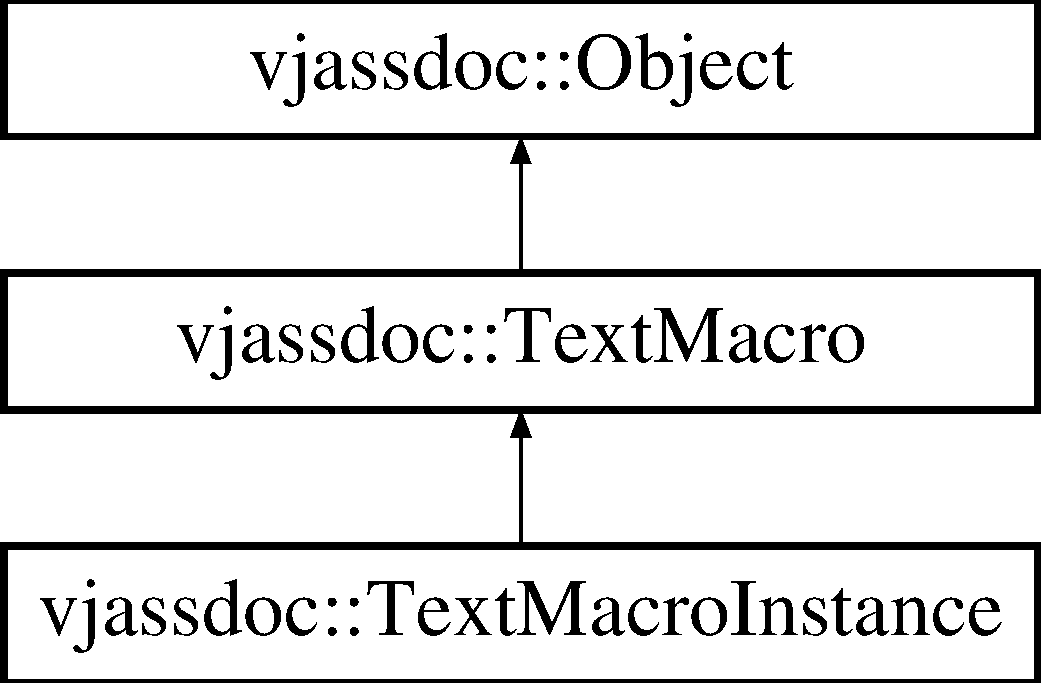
\includegraphics[height=3cm]{classvjassdoc_1_1TextMacroInstance}
\end{center}
\end{figure}
\subsection*{Public Member Functions}
\begin{CompactItemize}
\item 
\hyperlink{classvjassdoc_1_1TextMacroInstance_e6f4e775e305ef77a1952b6ff909193d}{TextMacroInstance} (const std::string \&identifier, class \hyperlink{classvjassdoc_1_1SourceFile}{SourceFile} $\ast$sourceFile, unsigned int line, class \hyperlink{classvjassdoc_1_1DocComment}{DocComment} $\ast$docComment, const std::string \&arguments)
\item 
\hyperlink{classvjassdoc_1_1TextMacroInstance_7bd68ef5afcd884b1802e5b4dbaf829d}{TextMacroInstance} (std::vector$<$ const unsigned char $\ast$ $>$ \&columnVector)
\item 
virtual void \hyperlink{classvjassdoc_1_1TextMacroInstance_e60b03ce172f8eefde2cdcc31533ee2d}{init} ()
\item 
virtual void \hyperlink{classvjassdoc_1_1TextMacroInstance_2bc8e5c94f5a74795d0c2d8137522d89}{pageNavigation} (std::ofstream \&file) const 
\item 
virtual void \hyperlink{classvjassdoc_1_1TextMacroInstance_4785937fa62c12f3586276a2d5dcbe52}{page} (std::ofstream \&file) const 
\item 
virtual std::string \hyperlink{classvjassdoc_1_1TextMacroInstance_7659e7ac5ff7547dfc526a4a7ff152b5}{sqlStatement} () const 
\item 
class \hyperlink{classvjassdoc_1_1TextMacro}{TextMacro} $\ast$ \hyperlink{classvjassdoc_1_1TextMacroInstance_2ad0f2fc0c5d03502e91899f6621edfc}{textMacro} () const 
\end{CompactItemize}


\subsection{Constructor \& Destructor Documentation}
\hypertarget{classvjassdoc_1_1TextMacroInstance_e6f4e775e305ef77a1952b6ff909193d}{
\index{vjassdoc::TextMacroInstance@{vjassdoc::TextMacroInstance}!TextMacroInstance@{TextMacroInstance}}
\index{TextMacroInstance@{TextMacroInstance}!vjassdoc::TextMacroInstance@{vjassdoc::TextMacroInstance}}
\subsubsection{\setlength{\rightskip}{0pt plus 5cm}vjassdoc::TextMacroInstance::TextMacroInstance (const std::string \& {\em identifier}, class {\bf SourceFile} $\ast$ {\em sourceFile}, unsigned int {\em line}, class {\bf DocComment} $\ast$ {\em docComment}, const std::string \& {\em arguments})}}
\label{classvjassdoc_1_1TextMacroInstance_e6f4e775e305ef77a1952b6ff909193d}


\hypertarget{classvjassdoc_1_1TextMacroInstance_7bd68ef5afcd884b1802e5b4dbaf829d}{
\index{vjassdoc::TextMacroInstance@{vjassdoc::TextMacroInstance}!TextMacroInstance@{TextMacroInstance}}
\index{TextMacroInstance@{TextMacroInstance}!vjassdoc::TextMacroInstance@{vjassdoc::TextMacroInstance}}
\subsubsection{\setlength{\rightskip}{0pt plus 5cm}vjassdoc::TextMacroInstance::TextMacroInstance (std::vector$<$ const unsigned char $\ast$ $>$ \& {\em columnVector})}}
\label{classvjassdoc_1_1TextMacroInstance_7bd68ef5afcd884b1802e5b4dbaf829d}




\subsection{Member Function Documentation}
\hypertarget{classvjassdoc_1_1TextMacroInstance_e60b03ce172f8eefde2cdcc31533ee2d}{
\index{vjassdoc::TextMacroInstance@{vjassdoc::TextMacroInstance}!init@{init}}
\index{init@{init}!vjassdoc::TextMacroInstance@{vjassdoc::TextMacroInstance}}
\subsubsection{\setlength{\rightskip}{0pt plus 5cm}void vjassdoc::TextMacroInstance::init ()\hspace{0.3cm}{\tt  \mbox{[}virtual\mbox{]}}}}
\label{classvjassdoc_1_1TextMacroInstance_e60b03ce172f8eefde2cdcc31533ee2d}




Reimplemented from \hyperlink{classvjassdoc_1_1TextMacro_816bdd2b838a4f1148ea17e5723e8577}{vjassdoc::TextMacro}.\hypertarget{classvjassdoc_1_1TextMacroInstance_2bc8e5c94f5a74795d0c2d8137522d89}{
\index{vjassdoc::TextMacroInstance@{vjassdoc::TextMacroInstance}!pageNavigation@{pageNavigation}}
\index{pageNavigation@{pageNavigation}!vjassdoc::TextMacroInstance@{vjassdoc::TextMacroInstance}}
\subsubsection{\setlength{\rightskip}{0pt plus 5cm}void vjassdoc::TextMacroInstance::pageNavigation (std::ofstream \& {\em file}) const\hspace{0.3cm}{\tt  \mbox{[}virtual\mbox{]}}}}
\label{classvjassdoc_1_1TextMacroInstance_2bc8e5c94f5a74795d0c2d8137522d89}




Reimplemented from \hyperlink{classvjassdoc_1_1TextMacro_d3ad5fe5300492db3d1aaf250d9b2a4b}{vjassdoc::TextMacro}.\hypertarget{classvjassdoc_1_1TextMacroInstance_4785937fa62c12f3586276a2d5dcbe52}{
\index{vjassdoc::TextMacroInstance@{vjassdoc::TextMacroInstance}!page@{page}}
\index{page@{page}!vjassdoc::TextMacroInstance@{vjassdoc::TextMacroInstance}}
\subsubsection{\setlength{\rightskip}{0pt plus 5cm}void vjassdoc::TextMacroInstance::page (std::ofstream \& {\em file}) const\hspace{0.3cm}{\tt  \mbox{[}virtual\mbox{]}}}}
\label{classvjassdoc_1_1TextMacroInstance_4785937fa62c12f3586276a2d5dcbe52}




Reimplemented from \hyperlink{classvjassdoc_1_1TextMacro_3336cdf9ad953dbd44b38fb14a2f73fa}{vjassdoc::TextMacro}.\hypertarget{classvjassdoc_1_1TextMacroInstance_7659e7ac5ff7547dfc526a4a7ff152b5}{
\index{vjassdoc::TextMacroInstance@{vjassdoc::TextMacroInstance}!sqlStatement@{sqlStatement}}
\index{sqlStatement@{sqlStatement}!vjassdoc::TextMacroInstance@{vjassdoc::TextMacroInstance}}
\subsubsection{\setlength{\rightskip}{0pt plus 5cm}std::string vjassdoc::TextMacroInstance::sqlStatement () const\hspace{0.3cm}{\tt  \mbox{[}virtual\mbox{]}}}}
\label{classvjassdoc_1_1TextMacroInstance_7659e7ac5ff7547dfc526a4a7ff152b5}




Reimplemented from \hyperlink{classvjassdoc_1_1TextMacro_e46c88feedc6197fbbae48de17f07366}{vjassdoc::TextMacro}.\hypertarget{classvjassdoc_1_1TextMacroInstance_2ad0f2fc0c5d03502e91899f6621edfc}{
\index{vjassdoc::TextMacroInstance@{vjassdoc::TextMacroInstance}!textMacro@{textMacro}}
\index{textMacro@{textMacro}!vjassdoc::TextMacroInstance@{vjassdoc::TextMacroInstance}}
\subsubsection{\setlength{\rightskip}{0pt plus 5cm}class {\bf TextMacro} $\ast$ vjassdoc::TextMacroInstance::textMacro () const\hspace{0.3cm}{\tt  \mbox{[}inline\mbox{]}}}}
\label{classvjassdoc_1_1TextMacroInstance_2ad0f2fc0c5d03502e91899f6621edfc}




The documentation for this class was generated from the following files:\begin{CompactItemize}
\item 
src/\hyperlink{textmacroinstance_8h}{textmacroinstance.h}\item 
src/\hyperlink{textmacroinstance_8cpp}{textmacroinstance.cpp}\end{CompactItemize}

\hypertarget{classvjassdoc_1_1Type}{
\section{vjassdoc::Type Class Reference}
\label{classvjassdoc_1_1Type}\index{vjassdoc::Type@{vjassdoc::Type}}
}
{\tt \#include $<$type.h$>$}

Inheritance diagram for vjassdoc::Type::\begin{figure}[H]
\begin{center}
\leavevmode
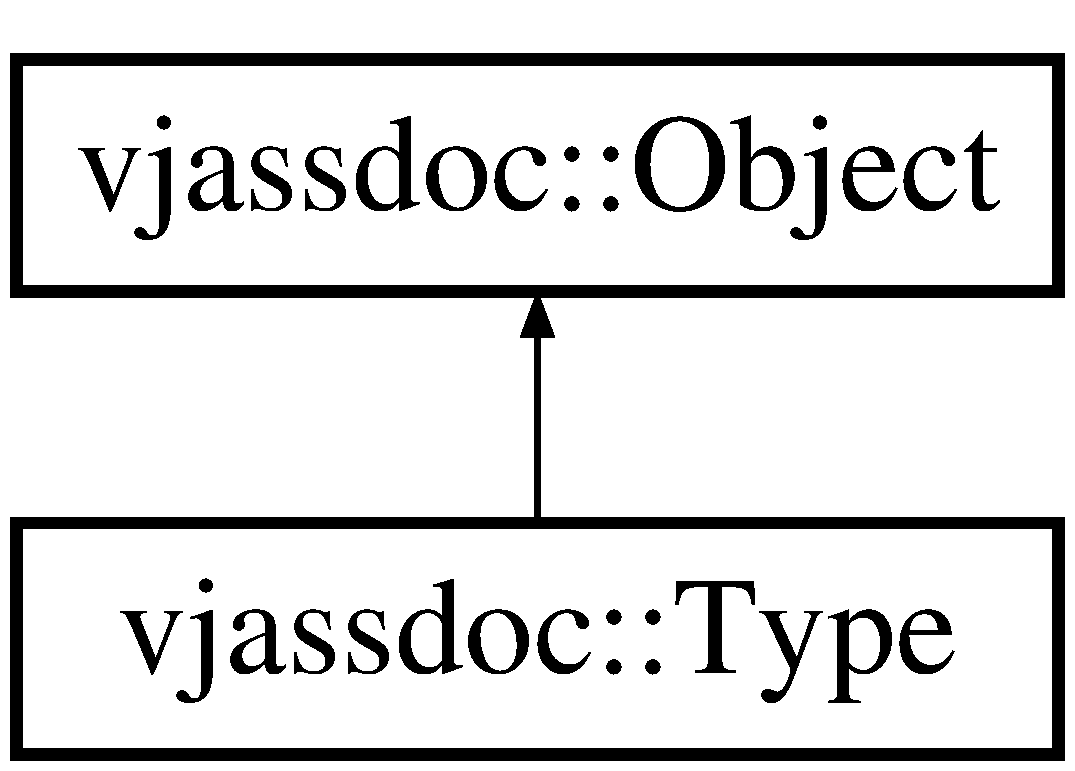
\includegraphics[height=2cm]{classvjassdoc_1_1Type}
\end{center}
\end{figure}
\subsection*{Public Member Functions}
\begin{CompactItemize}
\item 
\hyperlink{classvjassdoc_1_1Type_36d55cd487a11696b179790a299d5e09}{Type} (const std::string \&identifier, class \hyperlink{classvjassdoc_1_1SourceFile}{SourceFile} $\ast$sourceFile, unsigned int line, class \hyperlink{classvjassdoc_1_1DocComment}{DocComment} $\ast$docComment, const std::string \&typeExpression, const std::string \&sizeExpression)
\item 
\hyperlink{classvjassdoc_1_1Type_f1b3774bf65bd725e70182bc66650ce7}{Type} (std::vector$<$ const unsigned char $\ast$ $>$ \&columnVector)
\item 
virtual void \hyperlink{classvjassdoc_1_1Type_d4cadc76713790490c55be0bd0af1a1d}{init} ()
\item 
virtual void \hyperlink{classvjassdoc_1_1Type_bc514be419f91658df10d742c6999e47}{pageNavigation} (std::ofstream \&file) const 
\item 
virtual void \hyperlink{classvjassdoc_1_1Type_aa7a3044fc74587aa8800b1d67b18930}{page} (std::ofstream \&file) const 
\item 
virtual std::string \hyperlink{classvjassdoc_1_1Type_22741189ccde7fa7bc63abdeaf256c92}{sqlStatement} () const 
\item 
class \hyperlink{classvjassdoc_1_1Type}{Type} $\ast$ \hyperlink{classvjassdoc_1_1Type_e0527e578a64a9f6be29176281397397}{type} () const 
\item 
class \hyperlink{classvjassdoc_1_1Object}{Object} $\ast$ \hyperlink{classvjassdoc_1_1Type_93ddef89deb764de56905c9c78074c6f}{size} () const 
\item 
int \hyperlink{classvjassdoc_1_1Type_52c75b9b928f2027d83837fc7cb279a5}{sizeLiteral} () const 
\end{CompactItemize}


\subsection{Constructor \& Destructor Documentation}
\hypertarget{classvjassdoc_1_1Type_36d55cd487a11696b179790a299d5e09}{
\index{vjassdoc::Type@{vjassdoc::Type}!Type@{Type}}
\index{Type@{Type}!vjassdoc::Type@{vjassdoc::Type}}
\subsubsection{\setlength{\rightskip}{0pt plus 5cm}vjassdoc::Type::Type (const std::string \& {\em identifier}, class {\bf SourceFile} $\ast$ {\em sourceFile}, unsigned int {\em line}, class {\bf DocComment} $\ast$ {\em docComment}, const std::string \& {\em typeExpression}, const std::string \& {\em sizeExpression})}}
\label{classvjassdoc_1_1Type_36d55cd487a11696b179790a299d5e09}


\hypertarget{classvjassdoc_1_1Type_f1b3774bf65bd725e70182bc66650ce7}{
\index{vjassdoc::Type@{vjassdoc::Type}!Type@{Type}}
\index{Type@{Type}!vjassdoc::Type@{vjassdoc::Type}}
\subsubsection{\setlength{\rightskip}{0pt plus 5cm}vjassdoc::Type::Type (std::vector$<$ const unsigned char $\ast$ $>$ \& {\em columnVector})}}
\label{classvjassdoc_1_1Type_f1b3774bf65bd725e70182bc66650ce7}




\subsection{Member Function Documentation}
\hypertarget{classvjassdoc_1_1Type_d4cadc76713790490c55be0bd0af1a1d}{
\index{vjassdoc::Type@{vjassdoc::Type}!init@{init}}
\index{init@{init}!vjassdoc::Type@{vjassdoc::Type}}
\subsubsection{\setlength{\rightskip}{0pt plus 5cm}void vjassdoc::Type::init ()\hspace{0.3cm}{\tt  \mbox{[}virtual\mbox{]}}}}
\label{classvjassdoc_1_1Type_d4cadc76713790490c55be0bd0af1a1d}




Implements \hyperlink{classvjassdoc_1_1Object_bd43e77dbe80055f5adda67661dfaca4}{vjassdoc::Object}.\hypertarget{classvjassdoc_1_1Type_bc514be419f91658df10d742c6999e47}{
\index{vjassdoc::Type@{vjassdoc::Type}!pageNavigation@{pageNavigation}}
\index{pageNavigation@{pageNavigation}!vjassdoc::Type@{vjassdoc::Type}}
\subsubsection{\setlength{\rightskip}{0pt plus 5cm}void vjassdoc::Type::pageNavigation (std::ofstream \& {\em file}) const\hspace{0.3cm}{\tt  \mbox{[}virtual\mbox{]}}}}
\label{classvjassdoc_1_1Type_bc514be419f91658df10d742c6999e47}




Implements \hyperlink{classvjassdoc_1_1Object_736bbb6719edd8070d8f56c364a2764c}{vjassdoc::Object}.\hypertarget{classvjassdoc_1_1Type_aa7a3044fc74587aa8800b1d67b18930}{
\index{vjassdoc::Type@{vjassdoc::Type}!page@{page}}
\index{page@{page}!vjassdoc::Type@{vjassdoc::Type}}
\subsubsection{\setlength{\rightskip}{0pt plus 5cm}void vjassdoc::Type::page (std::ofstream \& {\em file}) const\hspace{0.3cm}{\tt  \mbox{[}virtual\mbox{]}}}}
\label{classvjassdoc_1_1Type_aa7a3044fc74587aa8800b1d67b18930}




Implements \hyperlink{classvjassdoc_1_1Object_a0489e38956f3507566b1bc6e3e2c8af}{vjassdoc::Object}.\hypertarget{classvjassdoc_1_1Type_22741189ccde7fa7bc63abdeaf256c92}{
\index{vjassdoc::Type@{vjassdoc::Type}!sqlStatement@{sqlStatement}}
\index{sqlStatement@{sqlStatement}!vjassdoc::Type@{vjassdoc::Type}}
\subsubsection{\setlength{\rightskip}{0pt plus 5cm}std::string vjassdoc::Type::sqlStatement () const\hspace{0.3cm}{\tt  \mbox{[}virtual\mbox{]}}}}
\label{classvjassdoc_1_1Type_22741189ccde7fa7bc63abdeaf256c92}




Reimplemented from \hyperlink{classvjassdoc_1_1Object_4e8ebbb0ce5b0bf91ec847b1e4a9f8fc}{vjassdoc::Object}.\hypertarget{classvjassdoc_1_1Type_e0527e578a64a9f6be29176281397397}{
\index{vjassdoc::Type@{vjassdoc::Type}!type@{type}}
\index{type@{type}!vjassdoc::Type@{vjassdoc::Type}}
\subsubsection{\setlength{\rightskip}{0pt plus 5cm}class {\bf Type} $\ast$ vjassdoc::Type::type () const\hspace{0.3cm}{\tt  \mbox{[}inline\mbox{]}}}}
\label{classvjassdoc_1_1Type_e0527e578a64a9f6be29176281397397}


\hypertarget{classvjassdoc_1_1Type_93ddef89deb764de56905c9c78074c6f}{
\index{vjassdoc::Type@{vjassdoc::Type}!size@{size}}
\index{size@{size}!vjassdoc::Type@{vjassdoc::Type}}
\subsubsection{\setlength{\rightskip}{0pt plus 5cm}class {\bf Object} $\ast$ vjassdoc::Type::size () const\hspace{0.3cm}{\tt  \mbox{[}inline\mbox{]}}}}
\label{classvjassdoc_1_1Type_93ddef89deb764de56905c9c78074c6f}


\hypertarget{classvjassdoc_1_1Type_52c75b9b928f2027d83837fc7cb279a5}{
\index{vjassdoc::Type@{vjassdoc::Type}!sizeLiteral@{sizeLiteral}}
\index{sizeLiteral@{sizeLiteral}!vjassdoc::Type@{vjassdoc::Type}}
\subsubsection{\setlength{\rightskip}{0pt plus 5cm}int vjassdoc::Type::sizeLiteral () const\hspace{0.3cm}{\tt  \mbox{[}inline\mbox{]}}}}
\label{classvjassdoc_1_1Type_52c75b9b928f2027d83837fc7cb279a5}


If the size is not an object it may be an integer value. \begin{Desc}
\item[Returns:]Returns the size. If the type has no size this value will be -1. \end{Desc}


The documentation for this class was generated from the following files:\begin{CompactItemize}
\item 
src/\hyperlink{type_8h}{type.h}\item 
src/\hyperlink{type_8cpp}{type.cpp}\end{CompactItemize}

\hypertarget{classvjassdoc_1_1Vjassdoc}{
\section{vjassdoc::Vjassdoc Class Reference}
\label{classvjassdoc_1_1Vjassdoc}\index{vjassdoc::Vjassdoc@{vjassdoc::Vjassdoc}}
}
{\tt \#include $<$vjassdoc.h$>$}

\subsection*{Static Public Member Functions}
\begin{CompactItemize}
\item 
static void \hyperlink{classvjassdoc_1_1Vjassdoc_73090a0eeffae1af73d153b881fd5d03}{run} (bool jass, bool debug, bool privateSpace, bool textmacros, bool html, bool pages, bool specialPages, bool database, bool verbose, bool time, bool alphabetical, bool parseObjectsOfList\mbox{[}Parser::MaxLists\mbox{]}, const std::string \&title, const std::string \&dir, std::list$<$ std::string $>$ $\ast$importDirs, std::list$<$ std::string $>$ $\ast$filePaths)
\item 
static class \hyperlink{classvjassdoc_1_1Parser}{Parser} $\ast$ \hyperlink{classvjassdoc_1_1Vjassdoc_b8697267d6b9ad377e05fba7132ca804}{getParser} ()
\item 
static bool \hyperlink{classvjassdoc_1_1Vjassdoc_1fe1b4e1b45efef8687def4cb833f70f}{jassOnly} ()
\item 
static bool \hyperlink{classvjassdoc_1_1Vjassdoc_25d13d1e5ffe741f3f457cce5101739e}{useDebugMode} ()
\item 
static bool \hyperlink{classvjassdoc_1_1Vjassdoc_e4a75f16d2c7258ee5d9ac3c8e049d69}{parsePrivateSpace} ()
\item 
static bool \hyperlink{classvjassdoc_1_1Vjassdoc_3400f429e29c73d57175b5f4f46d3af2}{parseTextMacroSpace} ()
\item 
static bool \hyperlink{classvjassdoc_1_1Vjassdoc_57da4b736dceace2c0db1aafaf6aa315}{saveAsHtml} ()
\item 
static bool \hyperlink{classvjassdoc_1_1Vjassdoc_6b0ac828b1d3214995b915d81fb3f8dd}{createPages} ()
\item 
static bool \hyperlink{classvjassdoc_1_1Vjassdoc_6356b84d6992625cd9100448f90957e0}{createSpecialPages} ()
\item 
static bool \hyperlink{classvjassdoc_1_1Vjassdoc_31b8f8e1823617f4bdbe49ca4dca1f35}{createDatabase} ()
\item 
static bool \hyperlink{classvjassdoc_1_1Vjassdoc_def212f6d705e55cab5211271e63a6a0}{showVerbose} ()
\item 
static bool \hyperlink{classvjassdoc_1_1Vjassdoc_6c9c4ca961a2c19801261be4c6f1922c}{sortAlphabetically} ()
\item 
static bool \hyperlink{classvjassdoc_1_1Vjassdoc_d4502ac69ac8bd526d813606a7081d41}{shouldParseObjectsOfList} (const enum \hyperlink{classvjassdoc_1_1Parser_4ef39527519272daf05a22b5276062ad}{Parser::List} \&list)
\item 
static std::string \hyperlink{classvjassdoc_1_1Vjassdoc_7ba3ab042719acc2ca719ea6936345bc}{getTitle} ()
\item 
static std::string \hyperlink{classvjassdoc_1_1Vjassdoc_212f33c8cf9c9be734cfbf9cfb040025}{getDir} ()
\item 
static std::list$<$ std::string $>$ $\ast$ \hyperlink{classvjassdoc_1_1Vjassdoc_556e1fe15a58becec3da4e281bf73f09}{getImportDirs} ()
\item 
static std::list$<$ std::string $>$ $\ast$ \hyperlink{classvjassdoc_1_1Vjassdoc_6b27e1cf9a3a03f9d8d2157e4b831a29}{getFilePaths} ()
\item 
static void \hyperlink{classvjassdoc_1_1Vjassdoc_af08606e734200e4c99860a6867216e5}{addLines} (const unsigned int \&addedLines)
\item 
static void \hyperlink{classvjassdoc_1_1Vjassdoc_7aa83fb64697927220f66616cf30e982}{addFile} ()
\item 
static unsigned int \hyperlink{classvjassdoc_1_1Vjassdoc_c0b832c86853f4f65c4eb28150808658}{getFiles} ()
\end{CompactItemize}
\subsection*{Static Public Attributes}
\begin{CompactItemize}
\item 
static const char $\ast$ \hyperlink{classvjassdoc_1_1Vjassdoc_229bee6b4735e83a9a28b98eb4650eef}{version} = \char`\"{}0.2.3\char`\"{}
\item 
static const char $\ast$ \hyperlink{classvjassdoc_1_1Vjassdoc_f3b3e3dfe26a57385265f8ba0d4fef16}{dirSeparator}
\end{CompactItemize}


\subsection{Member Function Documentation}
\hypertarget{classvjassdoc_1_1Vjassdoc_73090a0eeffae1af73d153b881fd5d03}{
\index{vjassdoc::Vjassdoc@{vjassdoc::Vjassdoc}!run@{run}}
\index{run@{run}!vjassdoc::Vjassdoc@{vjassdoc::Vjassdoc}}
\subsubsection{\setlength{\rightskip}{0pt plus 5cm}void vjassdoc::Vjassdoc::run (bool {\em jass}, bool {\em debug}, bool {\em privateSpace}, bool {\em textmacros}, bool {\em html}, bool {\em pages}, bool {\em specialPages}, bool {\em database}, bool {\em verbose}, bool {\em time}, bool {\em alphabetical}, bool {\em parseObjectsOfList}\mbox{[}Parser::MaxLists\mbox{]}, const std::string \& {\em title}, const std::string \& {\em dir}, std::list$<$ std::string $>$ $\ast$ {\em importDirs}, std::list$<$ std::string $>$ $\ast$ {\em filePaths})\hspace{0.3cm}{\tt  \mbox{[}static\mbox{]}}}}
\label{classvjassdoc_1_1Vjassdoc_73090a0eeffae1af73d153b881fd5d03}


\hypertarget{classvjassdoc_1_1Vjassdoc_b8697267d6b9ad377e05fba7132ca804}{
\index{vjassdoc::Vjassdoc@{vjassdoc::Vjassdoc}!getParser@{getParser}}
\index{getParser@{getParser}!vjassdoc::Vjassdoc@{vjassdoc::Vjassdoc}}
\subsubsection{\setlength{\rightskip}{0pt plus 5cm}{\bf Parser} $\ast$ vjassdoc::Vjassdoc::getParser ()\hspace{0.3cm}{\tt  \mbox{[}inline, static\mbox{]}}}}
\label{classvjassdoc_1_1Vjassdoc_b8697267d6b9ad377e05fba7132ca804}


\hypertarget{classvjassdoc_1_1Vjassdoc_1fe1b4e1b45efef8687def4cb833f70f}{
\index{vjassdoc::Vjassdoc@{vjassdoc::Vjassdoc}!jassOnly@{jassOnly}}
\index{jassOnly@{jassOnly}!vjassdoc::Vjassdoc@{vjassdoc::Vjassdoc}}
\subsubsection{\setlength{\rightskip}{0pt plus 5cm}bool vjassdoc::Vjassdoc::jassOnly ()\hspace{0.3cm}{\tt  \mbox{[}inline, static\mbox{]}}}}
\label{classvjassdoc_1_1Vjassdoc_1fe1b4e1b45efef8687def4cb833f70f}


\hypertarget{classvjassdoc_1_1Vjassdoc_25d13d1e5ffe741f3f457cce5101739e}{
\index{vjassdoc::Vjassdoc@{vjassdoc::Vjassdoc}!useDebugMode@{useDebugMode}}
\index{useDebugMode@{useDebugMode}!vjassdoc::Vjassdoc@{vjassdoc::Vjassdoc}}
\subsubsection{\setlength{\rightskip}{0pt plus 5cm}bool vjassdoc::Vjassdoc::useDebugMode ()\hspace{0.3cm}{\tt  \mbox{[}inline, static\mbox{]}}}}
\label{classvjassdoc_1_1Vjassdoc_25d13d1e5ffe741f3f457cce5101739e}


\hypertarget{classvjassdoc_1_1Vjassdoc_e4a75f16d2c7258ee5d9ac3c8e049d69}{
\index{vjassdoc::Vjassdoc@{vjassdoc::Vjassdoc}!parsePrivateSpace@{parsePrivateSpace}}
\index{parsePrivateSpace@{parsePrivateSpace}!vjassdoc::Vjassdoc@{vjassdoc::Vjassdoc}}
\subsubsection{\setlength{\rightskip}{0pt plus 5cm}bool vjassdoc::Vjassdoc::parsePrivateSpace ()\hspace{0.3cm}{\tt  \mbox{[}inline, static\mbox{]}}}}
\label{classvjassdoc_1_1Vjassdoc_e4a75f16d2c7258ee5d9ac3c8e049d69}


\hypertarget{classvjassdoc_1_1Vjassdoc_3400f429e29c73d57175b5f4f46d3af2}{
\index{vjassdoc::Vjassdoc@{vjassdoc::Vjassdoc}!parseTextMacroSpace@{parseTextMacroSpace}}
\index{parseTextMacroSpace@{parseTextMacroSpace}!vjassdoc::Vjassdoc@{vjassdoc::Vjassdoc}}
\subsubsection{\setlength{\rightskip}{0pt plus 5cm}bool vjassdoc::Vjassdoc::parseTextMacroSpace ()\hspace{0.3cm}{\tt  \mbox{[}inline, static\mbox{]}}}}
\label{classvjassdoc_1_1Vjassdoc_3400f429e29c73d57175b5f4f46d3af2}


\hypertarget{classvjassdoc_1_1Vjassdoc_57da4b736dceace2c0db1aafaf6aa315}{
\index{vjassdoc::Vjassdoc@{vjassdoc::Vjassdoc}!saveAsHtml@{saveAsHtml}}
\index{saveAsHtml@{saveAsHtml}!vjassdoc::Vjassdoc@{vjassdoc::Vjassdoc}}
\subsubsection{\setlength{\rightskip}{0pt plus 5cm}bool vjassdoc::Vjassdoc::saveAsHtml ()\hspace{0.3cm}{\tt  \mbox{[}inline, static\mbox{]}}}}
\label{classvjassdoc_1_1Vjassdoc_57da4b736dceace2c0db1aafaf6aa315}


\hypertarget{classvjassdoc_1_1Vjassdoc_6b0ac828b1d3214995b915d81fb3f8dd}{
\index{vjassdoc::Vjassdoc@{vjassdoc::Vjassdoc}!createPages@{createPages}}
\index{createPages@{createPages}!vjassdoc::Vjassdoc@{vjassdoc::Vjassdoc}}
\subsubsection{\setlength{\rightskip}{0pt plus 5cm}bool vjassdoc::Vjassdoc::createPages ()\hspace{0.3cm}{\tt  \mbox{[}inline, static\mbox{]}}}}
\label{classvjassdoc_1_1Vjassdoc_6b0ac828b1d3214995b915d81fb3f8dd}


\hypertarget{classvjassdoc_1_1Vjassdoc_6356b84d6992625cd9100448f90957e0}{
\index{vjassdoc::Vjassdoc@{vjassdoc::Vjassdoc}!createSpecialPages@{createSpecialPages}}
\index{createSpecialPages@{createSpecialPages}!vjassdoc::Vjassdoc@{vjassdoc::Vjassdoc}}
\subsubsection{\setlength{\rightskip}{0pt plus 5cm}bool vjassdoc::Vjassdoc::createSpecialPages ()\hspace{0.3cm}{\tt  \mbox{[}inline, static\mbox{]}}}}
\label{classvjassdoc_1_1Vjassdoc_6356b84d6992625cd9100448f90957e0}


\hypertarget{classvjassdoc_1_1Vjassdoc_31b8f8e1823617f4bdbe49ca4dca1f35}{
\index{vjassdoc::Vjassdoc@{vjassdoc::Vjassdoc}!createDatabase@{createDatabase}}
\index{createDatabase@{createDatabase}!vjassdoc::Vjassdoc@{vjassdoc::Vjassdoc}}
\subsubsection{\setlength{\rightskip}{0pt plus 5cm}bool vjassdoc::Vjassdoc::createDatabase ()\hspace{0.3cm}{\tt  \mbox{[}inline, static\mbox{]}}}}
\label{classvjassdoc_1_1Vjassdoc_31b8f8e1823617f4bdbe49ca4dca1f35}


\hypertarget{classvjassdoc_1_1Vjassdoc_def212f6d705e55cab5211271e63a6a0}{
\index{vjassdoc::Vjassdoc@{vjassdoc::Vjassdoc}!showVerbose@{showVerbose}}
\index{showVerbose@{showVerbose}!vjassdoc::Vjassdoc@{vjassdoc::Vjassdoc}}
\subsubsection{\setlength{\rightskip}{0pt plus 5cm}bool vjassdoc::Vjassdoc::showVerbose ()\hspace{0.3cm}{\tt  \mbox{[}inline, static\mbox{]}}}}
\label{classvjassdoc_1_1Vjassdoc_def212f6d705e55cab5211271e63a6a0}


\hypertarget{classvjassdoc_1_1Vjassdoc_6c9c4ca961a2c19801261be4c6f1922c}{
\index{vjassdoc::Vjassdoc@{vjassdoc::Vjassdoc}!sortAlphabetically@{sortAlphabetically}}
\index{sortAlphabetically@{sortAlphabetically}!vjassdoc::Vjassdoc@{vjassdoc::Vjassdoc}}
\subsubsection{\setlength{\rightskip}{0pt plus 5cm}bool vjassdoc::Vjassdoc::sortAlphabetically ()\hspace{0.3cm}{\tt  \mbox{[}inline, static\mbox{]}}}}
\label{classvjassdoc_1_1Vjassdoc_6c9c4ca961a2c19801261be4c6f1922c}


\hypertarget{classvjassdoc_1_1Vjassdoc_d4502ac69ac8bd526d813606a7081d41}{
\index{vjassdoc::Vjassdoc@{vjassdoc::Vjassdoc}!shouldParseObjectsOfList@{shouldParseObjectsOfList}}
\index{shouldParseObjectsOfList@{shouldParseObjectsOfList}!vjassdoc::Vjassdoc@{vjassdoc::Vjassdoc}}
\subsubsection{\setlength{\rightskip}{0pt plus 5cm}bool vjassdoc::Vjassdoc::shouldParseObjectsOfList (const enum {\bf Parser::List} \& {\em list})\hspace{0.3cm}{\tt  \mbox{[}inline, static\mbox{]}}}}
\label{classvjassdoc_1_1Vjassdoc_d4502ac69ac8bd526d813606a7081d41}


\hypertarget{classvjassdoc_1_1Vjassdoc_7ba3ab042719acc2ca719ea6936345bc}{
\index{vjassdoc::Vjassdoc@{vjassdoc::Vjassdoc}!getTitle@{getTitle}}
\index{getTitle@{getTitle}!vjassdoc::Vjassdoc@{vjassdoc::Vjassdoc}}
\subsubsection{\setlength{\rightskip}{0pt plus 5cm}std::string vjassdoc::Vjassdoc::getTitle ()\hspace{0.3cm}{\tt  \mbox{[}inline, static\mbox{]}}}}
\label{classvjassdoc_1_1Vjassdoc_7ba3ab042719acc2ca719ea6936345bc}


\hypertarget{classvjassdoc_1_1Vjassdoc_212f33c8cf9c9be734cfbf9cfb040025}{
\index{vjassdoc::Vjassdoc@{vjassdoc::Vjassdoc}!getDir@{getDir}}
\index{getDir@{getDir}!vjassdoc::Vjassdoc@{vjassdoc::Vjassdoc}}
\subsubsection{\setlength{\rightskip}{0pt plus 5cm}std::string vjassdoc::Vjassdoc::getDir ()\hspace{0.3cm}{\tt  \mbox{[}inline, static\mbox{]}}}}
\label{classvjassdoc_1_1Vjassdoc_212f33c8cf9c9be734cfbf9cfb040025}


\hypertarget{classvjassdoc_1_1Vjassdoc_556e1fe15a58becec3da4e281bf73f09}{
\index{vjassdoc::Vjassdoc@{vjassdoc::Vjassdoc}!getImportDirs@{getImportDirs}}
\index{getImportDirs@{getImportDirs}!vjassdoc::Vjassdoc@{vjassdoc::Vjassdoc}}
\subsubsection{\setlength{\rightskip}{0pt plus 5cm}std::list$<$ std::string $>$ $\ast$ vjassdoc::Vjassdoc::getImportDirs ()\hspace{0.3cm}{\tt  \mbox{[}inline, static\mbox{]}}}}
\label{classvjassdoc_1_1Vjassdoc_556e1fe15a58becec3da4e281bf73f09}


\hypertarget{classvjassdoc_1_1Vjassdoc_6b27e1cf9a3a03f9d8d2157e4b831a29}{
\index{vjassdoc::Vjassdoc@{vjassdoc::Vjassdoc}!getFilePaths@{getFilePaths}}
\index{getFilePaths@{getFilePaths}!vjassdoc::Vjassdoc@{vjassdoc::Vjassdoc}}
\subsubsection{\setlength{\rightskip}{0pt plus 5cm}std::list$<$ std::string $>$ $\ast$ vjassdoc::Vjassdoc::getFilePaths ()\hspace{0.3cm}{\tt  \mbox{[}inline, static\mbox{]}}}}
\label{classvjassdoc_1_1Vjassdoc_6b27e1cf9a3a03f9d8d2157e4b831a29}


\hypertarget{classvjassdoc_1_1Vjassdoc_af08606e734200e4c99860a6867216e5}{
\index{vjassdoc::Vjassdoc@{vjassdoc::Vjassdoc}!addLines@{addLines}}
\index{addLines@{addLines}!vjassdoc::Vjassdoc@{vjassdoc::Vjassdoc}}
\subsubsection{\setlength{\rightskip}{0pt plus 5cm}void vjassdoc::Vjassdoc::addLines (const unsigned int \& {\em addedLines})\hspace{0.3cm}{\tt  \mbox{[}inline, static\mbox{]}}}}
\label{classvjassdoc_1_1Vjassdoc_af08606e734200e4c99860a6867216e5}


\hypertarget{classvjassdoc_1_1Vjassdoc_7aa83fb64697927220f66616cf30e982}{
\index{vjassdoc::Vjassdoc@{vjassdoc::Vjassdoc}!addFile@{addFile}}
\index{addFile@{addFile}!vjassdoc::Vjassdoc@{vjassdoc::Vjassdoc}}
\subsubsection{\setlength{\rightskip}{0pt plus 5cm}void vjassdoc::Vjassdoc::addFile ()\hspace{0.3cm}{\tt  \mbox{[}inline, static\mbox{]}}}}
\label{classvjassdoc_1_1Vjassdoc_7aa83fb64697927220f66616cf30e982}


\hypertarget{classvjassdoc_1_1Vjassdoc_c0b832c86853f4f65c4eb28150808658}{
\index{vjassdoc::Vjassdoc@{vjassdoc::Vjassdoc}!getFiles@{getFiles}}
\index{getFiles@{getFiles}!vjassdoc::Vjassdoc@{vjassdoc::Vjassdoc}}
\subsubsection{\setlength{\rightskip}{0pt plus 5cm}unsigned int vjassdoc::Vjassdoc::getFiles ()\hspace{0.3cm}{\tt  \mbox{[}inline, static\mbox{]}}}}
\label{classvjassdoc_1_1Vjassdoc_c0b832c86853f4f65c4eb28150808658}




\subsection{Member Data Documentation}
\hypertarget{classvjassdoc_1_1Vjassdoc_229bee6b4735e83a9a28b98eb4650eef}{
\index{vjassdoc::Vjassdoc@{vjassdoc::Vjassdoc}!version@{version}}
\index{version@{version}!vjassdoc::Vjassdoc@{vjassdoc::Vjassdoc}}
\subsubsection{\setlength{\rightskip}{0pt plus 5cm}const char $\ast$ {\bf vjassdoc::Vjassdoc::version} = \char`\"{}0.2.3\char`\"{}\hspace{0.3cm}{\tt  \mbox{[}static\mbox{]}}}}
\label{classvjassdoc_1_1Vjassdoc_229bee6b4735e83a9a28b98eb4650eef}


\hypertarget{classvjassdoc_1_1Vjassdoc_f3b3e3dfe26a57385265f8ba0d4fef16}{
\index{vjassdoc::Vjassdoc@{vjassdoc::Vjassdoc}!dirSeparator@{dirSeparator}}
\index{dirSeparator@{dirSeparator}!vjassdoc::Vjassdoc@{vjassdoc::Vjassdoc}}
\subsubsection{\setlength{\rightskip}{0pt plus 5cm}const char$\ast$ {\bf vjassdoc::Vjassdoc::dirSeparator}\hspace{0.3cm}{\tt  \mbox{[}static\mbox{]}}}}
\label{classvjassdoc_1_1Vjassdoc_f3b3e3dfe26a57385265f8ba0d4fef16}




The documentation for this class was generated from the following files:\begin{CompactItemize}
\item 
src/\hyperlink{vjassdoc_8h}{vjassdoc.h}\item 
src/\hyperlink{vjassdoc_8cpp}{vjassdoc.cpp}\end{CompactItemize}

\chapter{vjassdoc File Documentation}
\hypertarget{comment_8cpp}{
\section{src/comment.cpp File Reference}
\label{comment_8cpp}\index{src/comment.cpp@{src/comment.cpp}}
}
{\tt \#include $<$sstream$>$}\par
{\tt \#include \char`\"{}objects.h\char`\"{}}\par
{\tt \#include \char`\"{}internationalisation.h\char`\"{}}\par
\subsection*{Namespaces}
\begin{CompactItemize}
\item 
namespace \hyperlink{namespacevjassdoc}{vjassdoc}
\end{CompactItemize}

\hypertarget{comment_8h}{
\section{src/comment.h File Reference}
\label{comment_8h}\index{src/comment.h@{src/comment.h}}
}
{\tt \#include \char`\"{}object.h\char`\"{}}\par
\subsection*{Namespaces}
\begin{CompactItemize}
\item 
namespace \hyperlink{namespacevjassdoc}{vjassdoc}
\end{CompactItemize}
\subsection*{Classes}
\begin{CompactItemize}
\item 
class \hyperlink{classvjassdoc_1_1Comment}{vjassdoc::Comment}
\end{CompactItemize}

\hypertarget{doccomment_8cpp}{
\section{src/doccomment.cpp File Reference}
\label{doccomment_8cpp}\index{src/doccomment.cpp@{src/doccomment.cpp}}
}
{\tt \#include $<$iostream$>$}\par
{\tt \#include $<$sstream$>$}\par
{\tt \#include \char`\"{}objects.h\char`\"{}}\par
{\tt \#include \char`\"{}file.h\char`\"{}}\par
{\tt \#include \char`\"{}internationalisation.h\char`\"{}}\par
\subsection*{Namespaces}
\begin{CompactItemize}
\item 
namespace \hyperlink{namespacevjassdoc}{vjassdoc}
\end{CompactItemize}

\hypertarget{doccomment_8h}{
\section{src/doccomment.h File Reference}
\label{doccomment_8h}\index{src/doccomment.h@{src/doccomment.h}}
}
{\tt \#include \char`\"{}object.h\char`\"{}}\par
{\tt \#include \char`\"{}parser.h\char`\"{}}\par
\subsection*{Namespaces}
\begin{CompactItemize}
\item 
namespace \hyperlink{namespacevjassdoc}{vjassdoc}
\end{CompactItemize}
\subsection*{Classes}
\begin{CompactItemize}
\item 
class \hyperlink{classvjassdoc_1_1DocComment}{vjassdoc::DocComment}
\end{CompactItemize}

\hypertarget{file_8cpp}{
\section{src/file.cpp File Reference}
\label{file_8cpp}\index{src/file.cpp@{src/file.cpp}}
}
{\tt \#include $<$string$>$}\par
{\tt \#include $<$fstream$>$}\par
{\tt \#include $<$cstdio$>$}\par
{\tt \#include $<$iostream$>$}\par
{\tt \#include $<$sstream$>$}\par
{\tt \#include $<$list$>$}\par
{\tt \#include \char`\"{}file.h\char`\"{}}\par
{\tt \#include \char`\"{}vjassdoc.h\char`\"{}}\par
{\tt \#include \char`\"{}objects.h\char`\"{}}\par
{\tt \#include \char`\"{}parser.h\char`\"{}}\par
{\tt \#include \char`\"{}internationalisation.h\char`\"{}}\par
\subsection*{Namespaces}
\begin{CompactItemize}
\item 
namespace \hyperlink{namespacevjassdoc}{vjassdoc}
\end{CompactItemize}

\hypertarget{file_8h}{
\section{src/file.h File Reference}
\label{file_8h}\index{src/file.h@{src/file.h}}
}
{\tt \#include $<$list$>$}\par
{\tt \#include $<$string$>$}\par
{\tt \#include $<$fstream$>$}\par
\subsection*{Namespaces}
\begin{CompactItemize}
\item 
namespace \hyperlink{namespacevjassdoc}{vjassdoc}
\end{CompactItemize}
\subsection*{Classes}
\begin{CompactItemize}
\item 
class \hyperlink{classvjassdoc_1_1File}{vjassdoc::File}
\end{CompactItemize}

\hypertarget{function_8cpp}{
\section{src/function.cpp File Reference}
\label{function_8cpp}\index{src/function.cpp@{src/function.cpp}}
}
{\tt \#include $<$sstream$>$}\par
{\tt \#include \char`\"{}objects.h\char`\"{}}\par
{\tt \#include \char`\"{}internationalisation.h\char`\"{}}\par
\subsection*{Namespaces}
\begin{CompactItemize}
\item 
namespace \hyperlink{namespacevjassdoc}{vjassdoc}
\end{CompactItemize}

\hypertarget{function_8h}{
\section{src/function.h File Reference}
\label{function_8h}\index{src/function.h@{src/function.h}}
}
{\tt \#include \char`\"{}functioninterface.h\char`\"{}}\par
\subsection*{Namespaces}
\begin{CompactItemize}
\item 
namespace \hyperlink{namespacevjassdoc}{vjassdoc}
\end{CompactItemize}
\subsection*{Classes}
\begin{CompactItemize}
\item 
class \hyperlink{classvjassdoc_1_1Function}{vjassdoc::Function}
\end{CompactItemize}

\hypertarget{functioninterface_8cpp}{
\section{src/functioninterface.cpp File Reference}
\label{functioninterface_8cpp}\index{src/functioninterface.cpp@{src/functioninterface.cpp}}
}
{\tt \#include $<$sstream$>$}\par
{\tt \#include \char`\"{}objects.h\char`\"{}}\par
{\tt \#include \char`\"{}internationalisation.h\char`\"{}}\par
\subsection*{Namespaces}
\begin{CompactItemize}
\item 
namespace \hyperlink{namespacevjassdoc}{vjassdoc}
\end{CompactItemize}

\hypertarget{functioninterface_8h}{
\section{src/functioninterface.h File Reference}
\label{functioninterface_8h}\index{src/functioninterface.h@{src/functioninterface.h}}
}
{\tt \#include \char`\"{}object.h\char`\"{}}\par
\subsection*{Namespaces}
\begin{CompactItemize}
\item 
namespace \hyperlink{namespacevjassdoc}{vjassdoc}
\end{CompactItemize}
\subsection*{Classes}
\begin{CompactItemize}
\item 
class \hyperlink{classvjassdoc_1_1FunctionInterface}{vjassdoc::FunctionInterface}
\end{CompactItemize}

\hypertarget{global_8cpp}{
\section{src/global.cpp File Reference}
\label{global_8cpp}\index{src/global.cpp@{src/global.cpp}}
}
{\tt \#include $<$cctype$>$}\par
{\tt \#include $<$sstream$>$}\par
{\tt \#include \char`\"{}objects.h\char`\"{}}\par
{\tt \#include \char`\"{}vjassdoc.h\char`\"{}}\par
{\tt \#include \char`\"{}internationalisation.h\char`\"{}}\par
\subsection*{Namespaces}
\begin{CompactItemize}
\item 
namespace \hyperlink{namespacevjassdoc}{vjassdoc}
\end{CompactItemize}

\hypertarget{global_8h}{
\section{src/global.h File Reference}
\label{global_8h}\index{src/global.h@{src/global.h}}
}
{\tt \#include \char`\"{}object.h\char`\"{}}\par
\subsection*{Namespaces}
\begin{CompactItemize}
\item 
namespace \hyperlink{namespacevjassdoc}{vjassdoc}
\end{CompactItemize}
\subsection*{Classes}
\begin{CompactItemize}
\item 
class \hyperlink{classvjassdoc_1_1Global}{vjassdoc::Global}
\end{CompactItemize}

\hypertarget{interface_8cpp}{
\section{src/interface.cpp File Reference}
\label{interface_8cpp}\index{src/interface.cpp@{src/interface.cpp}}
}
{\tt \#include $<$sstream$>$}\par
{\tt \#include \char`\"{}objects.h\char`\"{}}\par
{\tt \#include \char`\"{}internationalisation.h\char`\"{}}\par
{\tt \#include \char`\"{}vjassdoc.h\char`\"{}}\par
\subsection*{Namespaces}
\begin{CompactItemize}
\item 
namespace \hyperlink{namespacevjassdoc}{vjassdoc}
\end{CompactItemize}

\hypertarget{interface_8h}{
\section{src/interface.h File Reference}
\label{interface_8h}\index{src/interface.h@{src/interface.h}}
}
{\tt \#include \char`\"{}object.h\char`\"{}}\par
\subsection*{Namespaces}
\begin{CompactItemize}
\item 
namespace \hyperlink{namespacevjassdoc}{vjassdoc}
\end{CompactItemize}
\subsection*{Classes}
\begin{CompactItemize}
\item 
class \hyperlink{classvjassdoc_1_1Interface}{vjassdoc::Interface}
\end{CompactItemize}

\hypertarget{internationalisation_8h}{
\section{src/internationalisation.h File Reference}
\label{internationalisation_8h}\index{src/internationalisation.h@{src/internationalisation.h}}
}
{\tt \#include $<$libintl.h$>$}\par
{\tt \#include $<$locale.h$>$}\par
\subsection*{Defines}
\begin{CompactItemize}
\item 
\#define \hyperlink{internationalisation_8h_a9bd4034a10d8f6a33b6c8e6416eac00}{\_\-}(string)~gettext(string)
\end{CompactItemize}


\subsection{Define Documentation}
\hypertarget{internationalisation_8h_a9bd4034a10d8f6a33b6c8e6416eac00}{
\index{internationalisation.h@{internationalisation.h}!\_\-@{\_\-}}
\index{\_\-@{\_\-}!internationalisation.h@{internationalisation.h}}
\subsubsection{\setlength{\rightskip}{0pt plus 5cm}\#define \_\-(string)~gettext(string)}}
\label{internationalisation_8h_a9bd4034a10d8f6a33b6c8e6416eac00}



\hypertarget{keyword_8cpp}{
\section{src/keyword.cpp File Reference}
\label{keyword_8cpp}\index{src/keyword.cpp@{src/keyword.cpp}}
}
{\tt \#include $<$sstream$>$}\par
{\tt \#include \char`\"{}objects.h\char`\"{}}\par
{\tt \#include \char`\"{}internationalisation.h\char`\"{}}\par
\subsection*{Namespaces}
\begin{CompactItemize}
\item 
namespace \hyperlink{namespacevjassdoc}{vjassdoc}
\end{CompactItemize}

\hypertarget{keyword_8h}{
\section{src/keyword.h File Reference}
\label{keyword_8h}\index{src/keyword.h@{src/keyword.h}}
}
{\tt \#include \char`\"{}object.h\char`\"{}}\par
\subsection*{Namespaces}
\begin{CompactItemize}
\item 
namespace \hyperlink{namespacevjassdoc}{vjassdoc}
\end{CompactItemize}
\subsection*{Classes}
\begin{CompactItemize}
\item 
class \hyperlink{classvjassdoc_1_1Keyword}{vjassdoc::Keyword}
\end{CompactItemize}

\hypertarget{library_8cpp}{
\section{src/library.cpp File Reference}
\label{library_8cpp}\index{src/library.cpp@{src/library.cpp}}
}
{\tt \#include $<$sstream$>$}\par
{\tt \#include $<$list$>$}\par
{\tt \#include \char`\"{}objects.h\char`\"{}}\par
{\tt \#include \char`\"{}internationalisation.h\char`\"{}}\par
{\tt \#include \char`\"{}vjassdoc.h\char`\"{}}\par
{\tt \#include \char`\"{}parser.h\char`\"{}}\par
\subsection*{Namespaces}
\begin{CompactItemize}
\item 
namespace \hyperlink{namespacevjassdoc}{vjassdoc}
\end{CompactItemize}

\hypertarget{library_8h}{
\section{src/library.h File Reference}
\label{library_8h}\index{src/library.h@{src/library.h}}
}
{\tt \#include \char`\"{}object.h\char`\"{}}\par
\subsection*{Namespaces}
\begin{CompactItemize}
\item 
namespace \hyperlink{namespacevjassdoc}{vjassdoc}
\end{CompactItemize}
\subsection*{Classes}
\begin{CompactItemize}
\item 
class \hyperlink{classvjassdoc_1_1Library}{vjassdoc::Library}
\end{CompactItemize}

\hypertarget{main_8cpp}{
\section{src/main.cpp File Reference}
\label{main_8cpp}\index{src/main.cpp@{src/main.cpp}}
}
{\tt \#include $<$iostream$>$}\par
{\tt \#include $<$string$>$}\par
{\tt \#include $<$cstdio$>$}\par
{\tt \#include $<$vector$>$}\par
{\tt \#include $<$list$>$}\par
{\tt \#include \char`\"{}internationalisation.h\char`\"{}}\par
{\tt \#include \char`\"{}vjassdoc.h\char`\"{}}\par
{\tt \#include \char`\"{}parser.h\char`\"{}}\par
\subsection*{Functions}
\begin{CompactItemize}
\item 
int \hyperlink{main_8cpp_0ddf1224851353fc92bfbff6f499fa97}{main} (int argc, char $\ast$argv\mbox{[}$\,$\mbox{]})
\end{CompactItemize}


\subsection{Function Documentation}
\hypertarget{main_8cpp_0ddf1224851353fc92bfbff6f499fa97}{
\index{main.cpp@{main.cpp}!main@{main}}
\index{main@{main}!main.cpp@{main.cpp}}
\subsubsection{\setlength{\rightskip}{0pt plus 5cm}int main (int {\em argc}, char $\ast$ {\em argv}\mbox{[}$\,$\mbox{]})}}
\label{main_8cpp_0ddf1224851353fc92bfbff6f499fa97}



\hypertarget{member_8cpp}{
\section{src/member.cpp File Reference}
\label{member_8cpp}\index{src/member.cpp@{src/member.cpp}}
}
{\tt \#include $<$sstream$>$}\par
{\tt \#include \char`\"{}objects.h\char`\"{}}\par
{\tt \#include \char`\"{}internationalisation.h\char`\"{}}\par
\subsection*{Namespaces}
\begin{CompactItemize}
\item 
namespace \hyperlink{namespacevjassdoc}{vjassdoc}
\end{CompactItemize}

\hypertarget{member_8h}{
\section{src/member.h File Reference}
\label{member_8h}\index{src/member.h@{src/member.h}}
}
{\tt \#include \char`\"{}global.h\char`\"{}}\par
\subsection*{Namespaces}
\begin{CompactItemize}
\item 
namespace \hyperlink{namespacevjassdoc}{vjassdoc}
\end{CompactItemize}
\subsection*{Classes}
\begin{CompactItemize}
\item 
class \hyperlink{classvjassdoc_1_1Member}{vjassdoc::Member}
\end{CompactItemize}

\hypertarget{method_8cpp}{
\section{src/method.cpp File Reference}
\label{method_8cpp}\index{src/method.cpp@{src/method.cpp}}
}
{\tt \#include $<$sstream$>$}\par
{\tt \#include \char`\"{}objects.h\char`\"{}}\par
{\tt \#include \char`\"{}internationalisation.h\char`\"{}}\par
\subsection*{Namespaces}
\begin{CompactItemize}
\item 
namespace \hyperlink{namespacevjassdoc}{vjassdoc}
\end{CompactItemize}

\hypertarget{method_8h}{
\section{src/method.h File Reference}
\label{method_8h}\index{src/method.h@{src/method.h}}
}
{\tt \#include \char`\"{}function.h\char`\"{}}\par
\subsection*{Namespaces}
\begin{CompactItemize}
\item 
namespace \hyperlink{namespacevjassdoc}{vjassdoc}
\end{CompactItemize}
\subsection*{Classes}
\begin{CompactItemize}
\item 
class \hyperlink{classvjassdoc_1_1Method}{vjassdoc::Method}
\end{CompactItemize}

\hypertarget{object_8cpp}{
\section{src/object.cpp File Reference}
\label{object_8cpp}\index{src/object.cpp@{src/object.cpp}}
}
{\tt \#include $<$sstream$>$}\par
{\tt \#include $<$cstdlib$>$}\par
{\tt \#include $<$cctype$>$}\par
{\tt \#include \char`\"{}objects.h\char`\"{}}\par
{\tt \#include \char`\"{}sourcefile.h\char`\"{}}\par
{\tt \#include \char`\"{}doccomment.h\char`\"{}}\par
{\tt \#include \char`\"{}vjassdoc.h\char`\"{}}\par
{\tt \#include \char`\"{}internationalisation.h\char`\"{}}\par
\subsection*{Namespaces}
\begin{CompactItemize}
\item 
namespace \hyperlink{namespacevjassdoc}{vjassdoc}
\end{CompactItemize}

\hypertarget{object_8h}{
\section{src/object.h File Reference}
\label{object_8h}\index{src/object.h@{src/object.h}}
}
{\tt \#include $<$string$>$}\par
{\tt \#include $<$vector$>$}\par
{\tt \#include $<$fstream$>$}\par
{\tt \#include $<$functional$>$}\par
{\tt \#include \char`\"{}parser.h\char`\"{}}\par
{\tt \#include \char`\"{}internationalisation.h\char`\"{}}\par
{\tt \#include \char`\"{}vjassdoc.h\char`\"{}}\par
\subsection*{Namespaces}
\begin{CompactItemize}
\item 
namespace \hyperlink{namespacevjassdoc}{vjassdoc}
\end{CompactItemize}
\subsection*{Classes}
\begin{CompactItemize}
\item 
class \hyperlink{classvjassdoc_1_1Object}{vjassdoc::Object}
\item 
struct \hyperlink{structvjassdoc_1_1Object_1_1AlphabeticalComparator}{vjassdoc::Object::AlphabeticalComparator}
\item 
struct \hyperlink{structvjassdoc_1_1Object_1_1IsInContainer}{vjassdoc::Object::IsInContainer}
\item 
struct \hyperlink{structvjassdoc_1_1Object_1_1IsInScope}{vjassdoc::Object::IsInScope}
\item 
struct \hyperlink{structvjassdoc_1_1Object_1_1IsInLibrary}{vjassdoc::Object::IsInLibrary}
\end{CompactItemize}

\hypertarget{objects_8h}{
\section{src/objects.h File Reference}
\label{objects_8h}\index{src/objects.h@{src/objects.h}}
}
{\tt \#include \char`\"{}object.h\char`\"{}}\par
{\tt \#include \char`\"{}comment.h\char`\"{}}\par
{\tt \#include \char`\"{}keyword.h\char`\"{}}\par
{\tt \#include \char`\"{}textmacro.h\char`\"{}}\par
{\tt \#include \char`\"{}textmacroinstance.h\char`\"{}}\par
{\tt \#include \char`\"{}type.h\char`\"{}}\par
{\tt \#include \char`\"{}global.h\char`\"{}}\par
{\tt \#include \char`\"{}member.h\char`\"{}}\par
{\tt \#include \char`\"{}functioninterface.h\char`\"{}}\par
{\tt \#include \char`\"{}function.h\char`\"{}}\par
{\tt \#include \char`\"{}method.h\char`\"{}}\par
{\tt \#include \char`\"{}interface.h\char`\"{}}\par
{\tt \#include \char`\"{}struct.h\char`\"{}}\par
{\tt \#include \char`\"{}scope.h\char`\"{}}\par
{\tt \#include \char`\"{}library.h\char`\"{}}\par
{\tt \#include \char`\"{}sourcefile.h\char`\"{}}\par
{\tt \#include \char`\"{}doccomment.h\char`\"{}}\par

\hypertarget{parser_8cpp}{
\section{src/parser.cpp File Reference}
\label{parser_8cpp}\index{src/parser.cpp@{src/parser.cpp}}
}
{\tt \#include $<$iostream$>$}\par
{\tt \#include $<$sstream$>$}\par
{\tt \#include $<$algorithm$>$}\par
{\tt \#include $<$fstream$>$}\par
{\tt \#include $<$sqlite3.h$>$}\par
{\tt \#include \char`\"{}parser.h\char`\"{}}\par
{\tt \#include \char`\"{}internationalisation.h\char`\"{}}\par
{\tt \#include \char`\"{}objects.h\char`\"{}}\par
{\tt \#include \char`\"{}vjassdoc.h\char`\"{}}\par
{\tt \#include \char`\"{}file.h\char`\"{}}\par
\subsection*{Namespaces}
\begin{CompactItemize}
\item 
namespace \hyperlink{namespacevjassdoc}{vjassdoc}
\end{CompactItemize}

\hypertarget{parser_8h}{
\section{src/parser.h File Reference}
\label{parser_8h}\index{src/parser.h@{src/parser.h}}
}
{\tt \#include $<$functional$>$}\par
{\tt \#include $<$list$>$}\par
{\tt \#include $<$string$>$}\par
{\tt \#include $<$sys/stat.h$>$}\par
{\tt \#include $<$sstream$>$}\par
{\tt \#include $<$vector$>$}\par
\subsection*{Namespaces}
\begin{CompactItemize}
\item 
namespace \hyperlink{namespacevjassdoc}{vjassdoc}
\end{CompactItemize}
\subsection*{Classes}
\begin{CompactItemize}
\item 
class \hyperlink{classvjassdoc_1_1Parser}{vjassdoc::Parser}
\item 
struct \hyperlink{structvjassdoc_1_1Parser_1_1Comparator}{vjassdoc::Parser::Comparator}
\item 
struct \textbf{vjassdoc::Parser::Database}
\end{CompactItemize}

\hypertarget{scope_8cpp}{
\section{src/scope.cpp File Reference}
\label{scope_8cpp}\index{src/scope.cpp@{src/scope.cpp}}
}
{\tt \#include $<$sstream$>$}\par
{\tt \#include \char`\"{}objects.h\char`\"{}}\par
{\tt \#include \char`\"{}internationalisation.h\char`\"{}}\par
\subsection*{Namespaces}
\begin{CompactItemize}
\item 
namespace \hyperlink{namespacevjassdoc}{vjassdoc}
\end{CompactItemize}

\hypertarget{scope_8h}{
\section{src/scope.h File Reference}
\label{scope_8h}\index{src/scope.h@{src/scope.h}}
}
{\tt \#include \char`\"{}object.h\char`\"{}}\par
\subsection*{Namespaces}
\begin{CompactItemize}
\item 
namespace \hyperlink{namespacevjassdoc}{vjassdoc}
\end{CompactItemize}
\subsection*{Classes}
\begin{CompactItemize}
\item 
class \hyperlink{classvjassdoc_1_1Scope}{vjassdoc::Scope}
\end{CompactItemize}

\hypertarget{sourcefile_8cpp}{
\section{src/sourcefile.cpp File Reference}
\label{sourcefile_8cpp}\index{src/sourcefile.cpp@{src/sourcefile.cpp}}
}
{\tt \#include $<$sstream$>$}\par
{\tt \#include \char`\"{}objects.h\char`\"{}}\par
{\tt \#include \char`\"{}internationalisation.h\char`\"{}}\par
\subsection*{Namespaces}
\begin{CompactItemize}
\item 
namespace \hyperlink{namespacevjassdoc}{vjassdoc}
\end{CompactItemize}

\hypertarget{sourcefile_8h}{
\section{src/sourcefile.h File Reference}
\label{sourcefile_8h}\index{src/sourcefile.h@{src/sourcefile.h}}
}
{\tt \#include \char`\"{}object.h\char`\"{}}\par
\subsection*{Namespaces}
\begin{CompactItemize}
\item 
namespace \hyperlink{namespacevjassdoc}{vjassdoc}
\end{CompactItemize}
\subsection*{Classes}
\begin{CompactItemize}
\item 
class \hyperlink{classvjassdoc_1_1SourceFile}{vjassdoc::SourceFile}
\end{CompactItemize}

\hypertarget{struct_8cpp}{
\section{src/struct.cpp File Reference}
\label{struct_8cpp}\index{src/struct.cpp@{src/struct.cpp}}
}
{\tt \#include $<$sstream$>$}\par
{\tt \#include \char`\"{}objects.h\char`\"{}}\par
{\tt \#include \char`\"{}file.h\char`\"{}}\par
{\tt \#include \char`\"{}internationalisation.h\char`\"{}}\par
{\tt \#include \char`\"{}vjassdoc.h\char`\"{}}\par
\subsection*{Namespaces}
\begin{CompactItemize}
\item 
namespace \hyperlink{namespacevjassdoc}{vjassdoc}
\end{CompactItemize}

\hypertarget{struct_8h}{
\section{src/struct.h File Reference}
\label{struct_8h}\index{src/struct.h@{src/struct.h}}
}
{\tt \#include \char`\"{}interface.h\char`\"{}}\par
\subsection*{Namespaces}
\begin{CompactItemize}
\item 
namespace \hyperlink{namespacevjassdoc}{vjassdoc}
\end{CompactItemize}
\subsection*{Classes}
\begin{CompactItemize}
\item 
class \hyperlink{classvjassdoc_1_1Struct}{vjassdoc::Struct}
\item 
struct \hyperlink{structvjassdoc_1_1Struct_1_1HasExtension}{vjassdoc::Struct::HasExtension}
\end{CompactItemize}

\hypertarget{textmacro_8cpp}{
\section{src/textmacro.cpp File Reference}
\label{textmacro_8cpp}\index{src/textmacro.cpp@{src/textmacro.cpp}}
}
{\tt \#include $<$sstream$>$}\par
{\tt \#include \char`\"{}objects.h\char`\"{}}\par
{\tt \#include \char`\"{}internationalisation.h\char`\"{}}\par
\subsection*{Namespaces}
\begin{CompactItemize}
\item 
namespace \hyperlink{namespacevjassdoc}{vjassdoc}
\end{CompactItemize}

\hypertarget{textmacro_8h}{
\section{src/textmacro.h File Reference}
\label{textmacro_8h}\index{src/textmacro.h@{src/textmacro.h}}
}
{\tt \#include \char`\"{}object.h\char`\"{}}\par
\subsection*{Namespaces}
\begin{CompactItemize}
\item 
namespace \hyperlink{namespacevjassdoc}{vjassdoc}
\end{CompactItemize}
\subsection*{Classes}
\begin{CompactItemize}
\item 
class \hyperlink{classvjassdoc_1_1TextMacro}{vjassdoc::TextMacro}
\end{CompactItemize}

\hypertarget{textmacroinstance_8cpp}{
\section{src/textmacroinstance.cpp File Reference}
\label{textmacroinstance_8cpp}\index{src/textmacroinstance.cpp@{src/textmacroinstance.cpp}}
}
{\tt \#include $<$sstream$>$}\par
{\tt \#include \char`\"{}objects.h\char`\"{}}\par
{\tt \#include \char`\"{}internationalisation.h\char`\"{}}\par
\subsection*{Namespaces}
\begin{CompactItemize}
\item 
namespace \hyperlink{namespacevjassdoc}{vjassdoc}
\end{CompactItemize}

\hypertarget{textmacroinstance_8h}{
\section{src/textmacroinstance.h File Reference}
\label{textmacroinstance_8h}\index{src/textmacroinstance.h@{src/textmacroinstance.h}}
}
{\tt \#include \char`\"{}textmacro.h\char`\"{}}\par
\subsection*{Namespaces}
\begin{CompactItemize}
\item 
namespace \hyperlink{namespacevjassdoc}{vjassdoc}
\end{CompactItemize}
\subsection*{Classes}
\begin{CompactItemize}
\item 
class \hyperlink{classvjassdoc_1_1TextMacroInstance}{vjassdoc::TextMacroInstance}
\end{CompactItemize}

\hypertarget{type_8cpp}{
\section{src/type.cpp File Reference}
\label{type_8cpp}\index{src/type.cpp@{src/type.cpp}}
}
{\tt \#include $<$cctype$>$}\par
{\tt \#include $<$sstream$>$}\par
{\tt \#include \char`\"{}objects.h\char`\"{}}\par
{\tt \#include \char`\"{}internationalisation.h\char`\"{}}\par
\subsection*{Namespaces}
\begin{CompactItemize}
\item 
namespace \hyperlink{namespacevjassdoc}{vjassdoc}
\end{CompactItemize}

\hypertarget{type_8h}{
\section{src/type.h File Reference}
\label{type_8h}\index{src/type.h@{src/type.h}}
}
{\tt \#include \char`\"{}object.h\char`\"{}}\par
\subsection*{Namespaces}
\begin{CompactItemize}
\item 
namespace \hyperlink{namespacevjassdoc}{vjassdoc}
\end{CompactItemize}
\subsection*{Classes}
\begin{CompactItemize}
\item 
class \hyperlink{classvjassdoc_1_1Type}{vjassdoc::Type}
\end{CompactItemize}

\hypertarget{vjassdoc_8cpp}{
\section{src/vjassdoc.cpp File Reference}
\label{vjassdoc_8cpp}\index{src/vjassdoc.cpp@{src/vjassdoc.cpp}}
}
{\tt \#include $<$sys/time.h$>$}\par
{\tt \#include $<$ctime$>$}\par
{\tt \#include $<$iostream$>$}\par
{\tt \#include $<$cstdio$>$}\par
{\tt \#include \char`\"{}vjassdoc.h\char`\"{}}\par
{\tt \#include \char`\"{}internationalisation.h\char`\"{}}\par
\subsection*{Namespaces}
\begin{CompactItemize}
\item 
namespace \hyperlink{namespacevjassdoc}{vjassdoc}
\end{CompactItemize}

\hypertarget{vjassdoc_8h}{
\section{src/vjassdoc.h File Reference}
\label{vjassdoc_8h}\index{src/vjassdoc.h@{src/vjassdoc.h}}
}
{\tt \#include $<$string$>$}\par
{\tt \#include $<$list$>$}\par
{\tt \#include \char`\"{}parser.h\char`\"{}}\par
\subsection*{Namespaces}
\begin{CompactItemize}
\item 
namespace \hyperlink{namespacevjassdoc}{vjassdoc}
\end{CompactItemize}
\subsection*{Classes}
\begin{CompactItemize}
\item 
class \hyperlink{classvjassdoc_1_1Vjassdoc}{vjassdoc::Vjassdoc}
\end{CompactItemize}

\chapter{vjassdoc Page Documentation}
\hypertarget{todo}{}\section{Todo List }\label{todo}
\label{todo__todo000001}
\hypertarget{todo__todo000001}{}
 \begin{description}
\item[Member \hyperlink{classvjassdoc_1_1DocComment_46ada773166611c9be898f74e0eb2315}{vjassdoc::DocComment::init}() ]FIXME \end{description}


\label{todo__todo000002}
\hypertarget{todo__todo000002}{}
 \begin{description}
\item[Member \hyperlink{classvjassdoc_1_1File_d35f0f273a4e7ecc96e4315edb842151}{vjassdoc::File::File}(const std::string \&filePath) ]Truncate the //! prefix \end{description}


\label{todo__todo000002}
\hypertarget{todo__todo000002}{}
 \begin{description}
\item[Member \hyperlink{classvjassdoc_1_1File_d35f0f273a4e7ecc96e4315edb842151}{vjassdoc::File::File}(const std::string \&filePath) ]Just close if good? \end{description}


\label{todo__todo000005}
\hypertarget{todo__todo000005}{}
 \begin{description}
\item[Member \hyperlink{classvjassdoc_1_1Object_b229c2eb3c0c7d1e86d789986bffe3f1}{vjassdoc::Object::sqlTableHeader}(const std::string \&tableName, const std::string \&entries) ]This function should be used to distribute all table header creations to their classes. \end{description}


\label{todo__todo000004}
\hypertarget{todo__todo000004}{}
 \begin{description}
\item[Member \hyperlink{classvjassdoc_1_1Object_e9ed6f9d16334a979405a9f2efab2239}{vjassdoc::Object::hasToSearchValueObject}(class Object $\ast$type, const std::string \&expression) ]Code type == null?! \end{description}


\label{todo__todo000006}
\hypertarget{todo__todo000006}{}
 \begin{description}
\item[Member \hyperlink{classvjassdoc_1_1Parser_25594f25b429a8ff7a4ed426ee0f3184}{vjassdoc::Parser::parse}() ]Test. \end{description}

\printindex
\end{document}
